%% 
%% Copyright 2007-2020 Elsevier Ltd
%% 
%% This file is part of the 'Elsarticle Bundle'.
%% ---------------------------------------------
%% 
%% It may be distributed under the conditions of the LaTeX Project Public
%% License, either version 1.2 of this license or (at your option) any
%% later version.  The latest version of this license is in
%%    http://www.latex-project.org/lppl.txt
%% and version 1.2 or later is part of all distributions of LaTeX
%% version 1999/12/01 or later.
%% 
%% The list of all files belonging to the 'Elsarticle Bundle' is
%% given in the file `manifest.txt'.
%% 
%% Template article for Elsevier's document class `elsarticle'
%% with harvard style bibliographic references

\documentclass[preprint,12pt]{elsarticle}

%% Use the option review to obtain double line spacing
%% \documentclass[preprint,review,12pt]{elsarticle}

%% Use the options 1p,twocolumn; 3p; 3p,twocolumn; 5p; or 5p,twocolumn
%% for a journal layout:
%% \documentclass[final,1p,times]{elsarticle}
%% \documentclass[final,1p,times,twocolumn]{elsarticle}
%% \documentclass[final,3p,times]{elsarticle}
%% \documentclass[final,3p,times,twocolumn]{elsarticle}
%% \documentclass[final,5p,times]{elsarticle}
%% \documentclass[final,5p,times,twocolumn]{elsarticle}

%% For including figures, graphicx.sty has been loaded in
%% elsarticle.cls. If you prefer to use the old commands
%% please give \usepackage{epsfig}

%% The amssymb package provides various useful mathematical symbols
\usepackage{amssymb}
%% The amsthm package provides extended theorem environments
%% \usepackage{amsthm}

%% The lineno packages adds line numbers. Start line numbering with
%% \begin{linenumbers}, end it with \end{linenumbers}. Or switch it on
%% for the whole article with \linenumbers.
%% \usepackage{lineno}
\usepackage{amsmath,mathtools}
\usepackage{gensymb}
\usepackage{booktabs}
\graphicspath{{figs/}}

\journal{Energy and AI}

\begin{document}

\begin{frontmatter}

%% Title, authors and addresses

%% use the tnoteref command within \title for footnotes;
%% use the tnotetext command for theassociated footnote;
%% use the fnref command within \author or \address for footnotes;
%% use the fntext command for theassociated footnote;
%% use the corref command within \author for corresponding author footnotes;
%% use the cortext command for theassociated footnote;
%% use the ead command for the email address,
%% and the form \ead[url] for the home page:
%% \title{Title\tnoteref{label1}}
%% \tnotetext[label1]{}
%% \author{Name\corref{cor1}\fnref{label2}}
%% \ead{email address}
%% \ead[url]{home page}
%% \fntext[label2]{}
%% \cortext[cor1]{}
%% \affiliation{organization={},
%%             addressline={},
%%             city={},
%%             postcode={},
%%             state={},
%%             country={}}
%% \fntext[label3]{}
\title{Coaxial multi-criteria optimization of a methane steam reforming reactor for effective hydrogen production and thermal management}

%% use optional labels to link authors explicitly to addresses:
%% \author[label1,label2]{}
%% \affiliation[label1]{organization={},
%%             addressline={},
%%             city={},
%%             postcode={},
%%             state={},
%%             country={}}
%%
%% \affiliation[label2]{organization={},
%%             addressline={},
%%             city={},
%%             postcode={},
%%             state={},
%%             country={}}


\author[affiliationA]{Marcin Pajak\corref{mycorrespondingauthor}}
\cortext[mycorrespondingauthor]{Corresponding author}
\ead{mpajak@agh.edu.pl}

\author[affiliationA]{Grzegorz Brus}

\author[affiliationA]{Janusz S. Szmyd}

\affiliation[affiliationA]{organization={AGH University of Science and Technology},
            city={Krakow},
            country={Poland}}

\begin{abstract}
The advancement in environmental awareness is the recent driving factor of the energy industry development. The market sentiments dictate the commercialization of unconventional energy sources. Thus, generation via hydrogen conversion gains popularity. The presented research regards the enhancement of the steam reforming reaction, used for the production of hydrogen via the conversion of hydrocarbons. The reforming process characterizes by a strong endothermic nature. The rapid course of the reaction leads to the creation of temperature gradients of a considerable magnitude. The presented research strives to alleviate the negative consequences of the reaction character. An original strategy by the name of macro-patterning is suggested as a remedy. The presented research proposes an updated concept, predicting the introduction of coaxial segments to the catalytic insert. The segments may consist of catalytic material or metallic foam applied for local suppression of the reaction. The morphology of specific segments may be altered independently, to allow for additional control of the reforming reaction. The objective of the research is to define the optimal segment composition. The optimization process is based on an in-house procedure implementing a genetic algorithm. The acquired results appear to validate the macro-pattering concept. A significant unification of the temperature field is obtained, with a simultaneous increase in hydrogen productivity.
\end{abstract}

%%Graphical abstract
\begin{graphicalabstract}
%\includegraphics{grabs}
\end{graphicalabstract}

%%Research highlights
\begin{highlights}
\item Introduction of a novel approach to the macro-patterning concept.
\item Sensitivity analysis conducted for the evolutionary algorithm parameters.
\item Enhancement of thermal conditions via a modification of the catalyst insert. 
\item Increase in hydrogen productivity. 
\end{highlights}

\begin{keyword}
hydrogen \sep evolutionary algorithms \sep reforming \sep design optimization
%% keywords here, in the form: keyword \sep keyword

%% PACS codes here, in the form: \PACS code \sep code

%% MSC codes here, in the form: \MSC code \sep code
%% or \MSC[2008] code \sep code (2000 is the default)

\end{keyword}

\end{frontmatter}

%% \linenumbers

\section{Introduction}

Hydrogen technologies are one of the promising directions of the clean energy sector development \cite{Qazi2022}. The research on hydrogen is conducted to provide a reliable alternative to the currently dominant fossil fuel energy sources \cite{Zou2016, Liobikiene2021}. Hydrogen might be used as an energy carrier for internal combustion or fuel cells, both resulting in steam being the main product \cite{Xu2020, Shadidi2021}.
 However, with the application of hydrogen technology, some crucial issues arise. The first issue regards hydrogen acquisition, as it does not occur on Earth in its pure form. The second matter is hydrogen storage, with currently no effective measures of long-term storage \cite{Hassan2021, Tarhan2022}.  The two most common processes for on-the-spot production of hydrogen are water electrolysis and the reforming of hydrocarbons  \cite{Hassan2021RSER, Azizan2020}. Water electrolysis is a process predicting the breaking of chemical bonds between oxygen and hydrogen in particles of water. The current state of the electrolysis development is far from meeting economical requirements \cite{Yukesh2021}. The only reasonable use of water electrolysis is to deplete surplus energy generated from renewable sources during low market demand and short-term storage of hydrogen for further use during increased demand for energy \cite{Chi2018}. The second measure for hydrogen production is the reforming reaction \cite{Zhang2021, Nkulikiyinka2020}. The reforming process is a catalytic reaction used for the conversion of hydrocarbons for the production of hydrogen \cite{Taherian2022, Faheem2022}. The reforming process can be successfully applied to the conversion of biofuels, allowing the reforming process to be considered a renewable hydrogen source \cite{Zhao2020, Gao2022}. Furthermore, the process can be successfully applied as a measure of carbohydrate-based waste gases or plastic recycling, establishing it as a prominent for hydrogen generation \cite{Saad2016, Zhang2022}. The reforming technology brings a series of issues regarding the thermal conditions occurring inside the reactor. The strong endothermic nature of the process results in the occurrence of thermal stresses and may lead to a shortening of the reactor's lifespan \cite{Mozdzierz2014}. The presented research aims to reduce the drawbacks of the process, by enhancement of the thermal conditions. The majority of researchers focused on the parametric study and optimization of the reaction conditions, resulting in improvements only to a certain extent \cite{Simpson2007, Naseri2015}. Further development of the process is pursued by the introduction of new materials and design concepts, including new catalyst structures \cite{Ali2016, Kolaczkowski2016}, the introduction of new kinds of catalyst supports \cite{Yadav2019}, or by rethinking the design of the reactor itself \cite{Butcher2014, Meloni2020, Cherif2022}.  A captivating opportunity is described in a work by Palma et al. \cite{Palma2017}, who introduced a structured catalyst for the intensification of the reforming reaction. The research confirms the improvement of the reaction rate, resulting from the enhancement of the axial and radial temperature distribution. The research reported by Yun et al. \cite{Yun2019}  focuses on the enhancement of heat transfer, by modification of the design, to acquire a maximized heat transfer area. The proper handling of heat in the reforming process is confirmed to enhance the overall process conduction \cite{Dubinin2018}.  Furthermore, a rapid temperature decay at the upstream region of the reactor results in thermal stresses forming in the reactor. Thus, leading to its uneven degradation and reduction of the unit's lifetime \cite{Mozdzierz2016}. A unification of the temperature distribution may not only improve the conditions but also achieve easier control of the process \cite{Mozdzierz2018}. The presented research aims to alleviate the negative consequences of the strong endothermic character of the process, via the introduction of radial division of the catalytic insert. The concept originates from the approach proposed by Settar et al. \cite{Settar2017}. The research predicted an introduction of macro-patterned active surfaces with an introduction of metallic foam matrices, focusing on providing advantageous thermal conditions for the reaction \cite{Settar2018a, Settar2018c}.  The presented research extends the concept to fill the whole reactor's volume with a catalytic composite of nickel and yttria-stabilized zirconia (Ni/YSZ), to maximize the reaction region in the reactor. Further, the reforming unit is divided into segments in the radial direction, instead of the longitudinal division \cite{Pajak2018}. Non-catalytic metallic foam is used as a substitute for parts of the catalyst, to adjust the intensity of the reaction proceeding, leading to the unification of the thermal field inside the reactor. To define the optimal alignment of the catalyst, an evolutionary algorithm is coupled with an in-house reforming simulation \cite{Pajak2021IJHEb}. The presented analysis includes:
 
 \begin{itemize}
 \item {Investigation of the macro-patterning concept applicability with the introduction of the catalytic insert radial division.}
 \item {Introduction of two separate principles for the configuration of the segments.}
 \item {Comprehensive sensitivity analysis to define the finest performing set of the evolutionary algorithm parameters.}
 \item {Analysis of the results robustness, via measuring the hydrogen productivity of specimens defined by the specific algorithms.}
 \end{itemize}

\section{Mathematical model}
\label{sec:math_model}

The reactor geometry is designed to allow modification of the insert in a real-life scenario. The analyzed process incorporates a plug-flow reactor, maintaining axial symmetry throughout its whole volume. The reactor consists of a straight, cylindrical pipe, allowing for an accessible replacement of the catalyst insert when required.  The introduced macro-patterning strategy predicts modification of the catalyst insert's morphology and its partial substitution with a non-catalytic material. Substitution of the catalyst material serves to enhance the heat transfer inside the reactor \cite{Pajak2018}. Metallic foams are chosen for application to the indicated issues \cite{Boomsma2003}. To provide a relevant measure for altering the temperature distribution inside the reactor, the catalyst insert is divided into segments. Each segment may consist of a catalyst or a non-catalytic material, with their morphological parameters individually assigned. The insert's segmentation is carried out according to two separate strategies. The first strategy predicts division in the radial direction with maintaining a constant width of inlet surfaces of each cylinder (Fig. \ref{fig:segments} b)). The second strategy predicts the application of segments with an identical area of the inlet surfaces for each of the coaxial cylinders (Fig. \ref{fig:segments} c)). The design is prepared to contain exclusively simple geometrical shapes, allowing to maintain an insignificant computational complexity of the domain \cite{Kaw2011}.  

\begin{figure}[h]
\centering
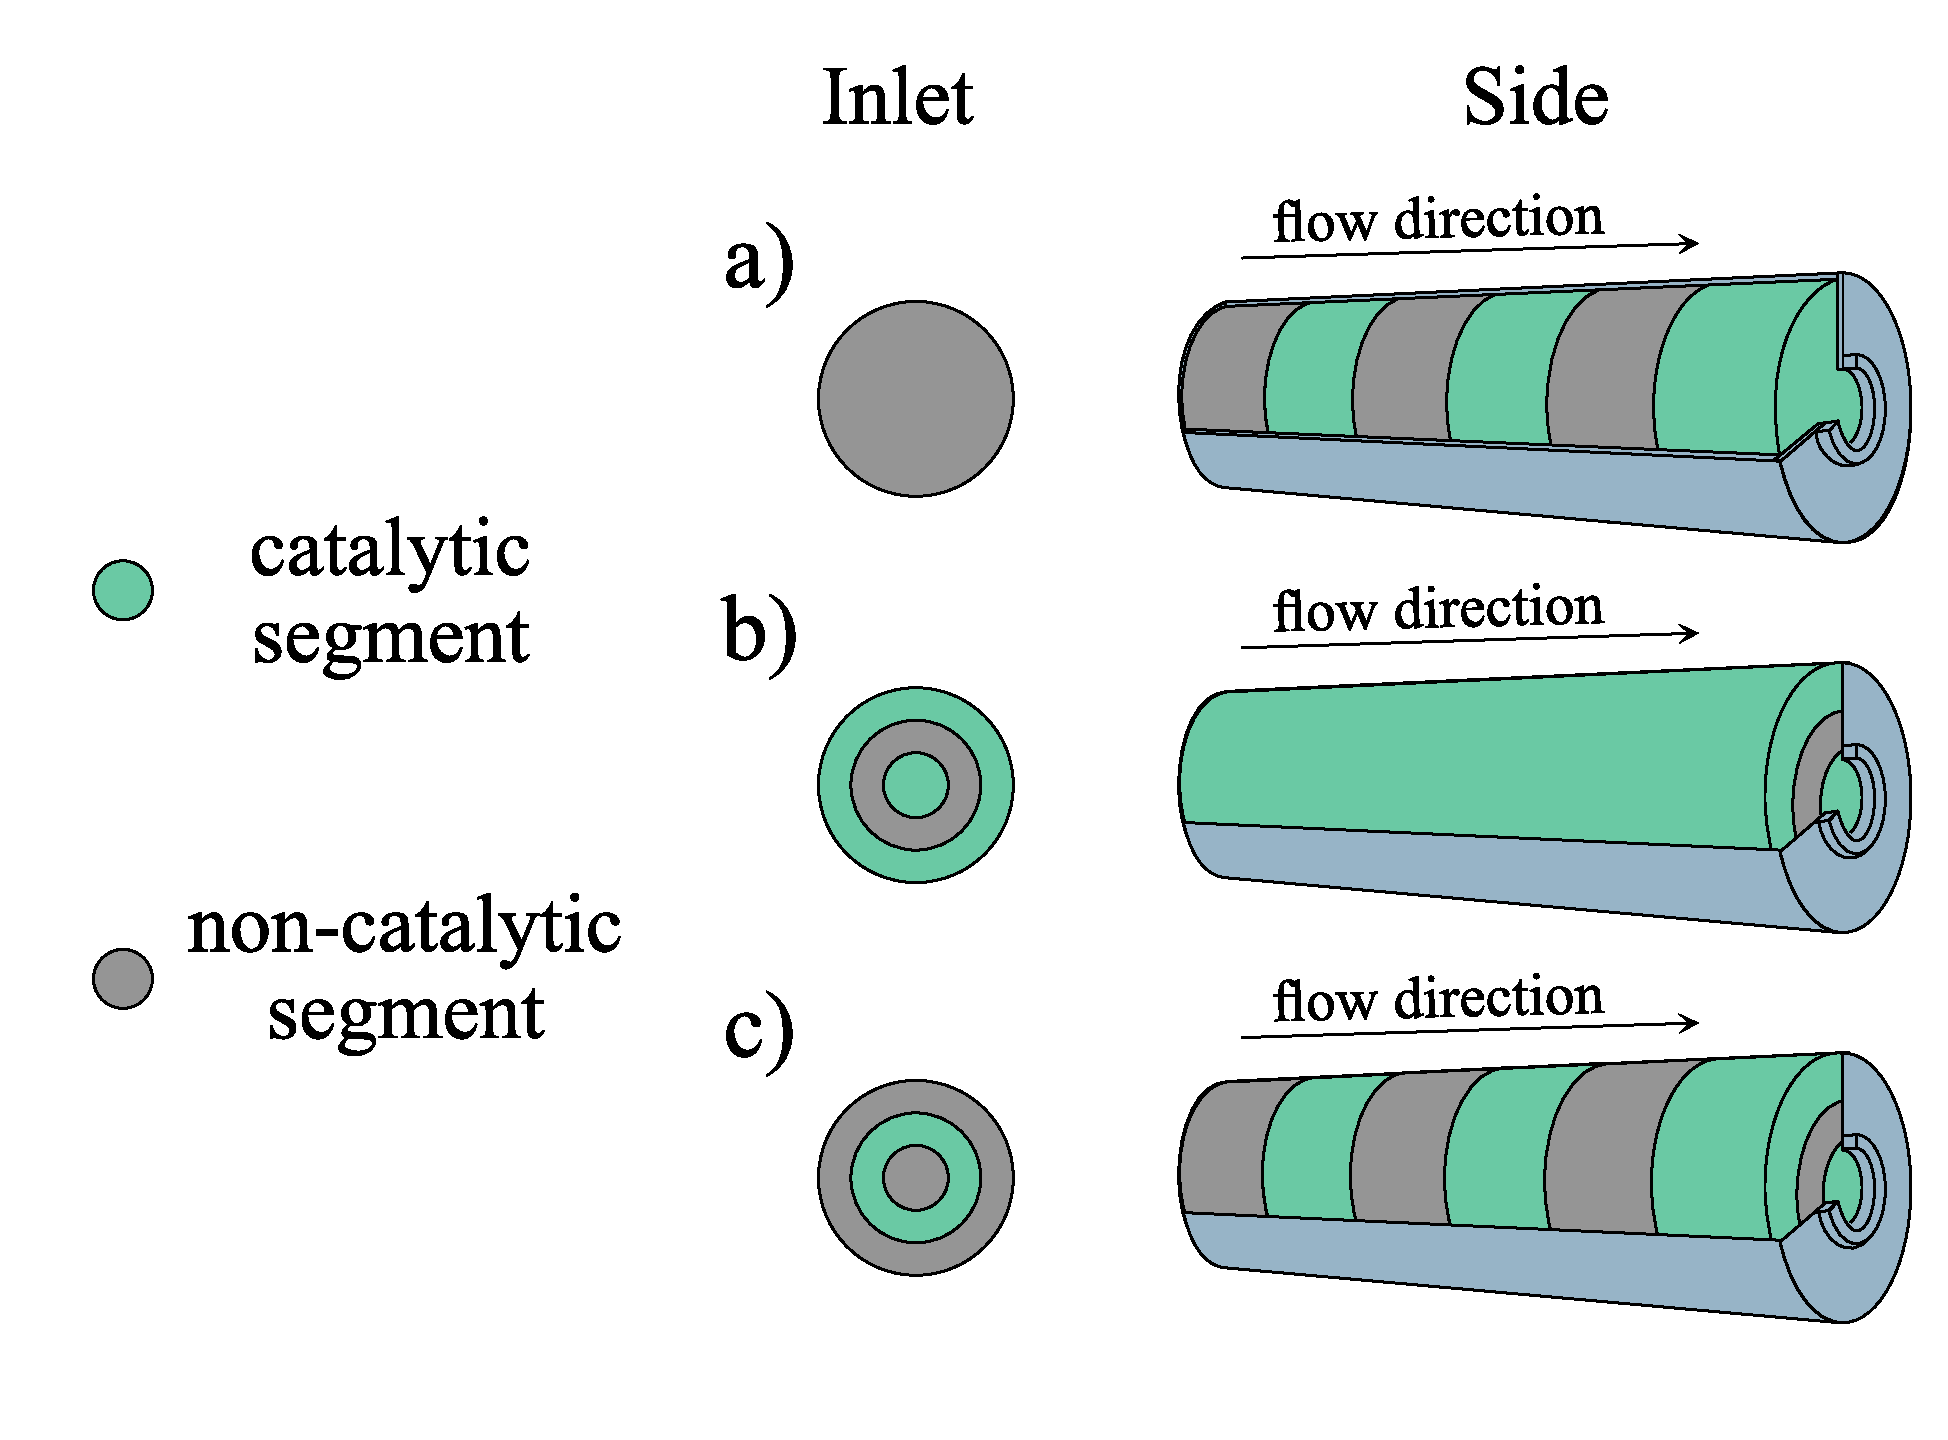
\includegraphics[width=120mm]{segments_concept.eps}\hspace{2pc} 
\caption{\label{fig:segments} The investigated macro-patterinig designs: a) conventional reactor with homogeneous and continuous catalytic insert, b) catalytic insert divided in the radial direction (equal width of inlet surface),  c) catalytic insert divided in the radial direction  (equal area of inlet surface)}
\end{figure}

\subsection{Chemical Reactions Model}
\label{subsec:math_model_ref}

The process is assumed to be dominated by three reactions, as reported in literature \cite{Xu1989, Komatsu2009, Mozdzierz2018}. The reactions are steam reforming of methane (MSR) (Eq. \eqref{eq:MSR}), dry reforming of methane (DRY) (Eq. \eqref{eq:DRY}), and water-gas shift reaction (WGS) (Eq. \eqref{eq:WGS}) \cite{Brus2015}. The stoichiometric equations for the reactions are presented below: 

\begin{multline}
\label{eq:MSR}
\hfill \rm{CH_{4}+H_2O \rightarrow	3H_2+CO}, \hfill\\
{\Delta H_{\rm{MSR}} = 206.1 \rm{\frac{kJ}{mol}},}
\end{multline}
\begin{multline}
\label{eq:DRY}
\hfill \rm{CH_4+CO_2 \rightleftharpoons 2H_2+2CO}, \hfill\\
{\Delta H_{\rm{DRY}} = 247 \rm{\frac{kJ}{mol}},}
\end{multline}
\begin{multline}
\label{eq:WGS}
\hfill \rm{CO+H_2O \rightleftharpoons H_2+CO_2}, \hfill\\
{\Delta H_{\rm{WGS}} = -41.15 \rm{\frac{kJ}{mol}}.}
\end{multline}

 The reformer is supplied with a mixture of H$_2$, CO$_2$, and CH$_4$. The exact composition of the inlet gases is determined by two parameters. The first is the steam-to-carbon ratio ($SC$), defining the ratio of steam to methane at the reactor's inlet. The second parameter is the carbon-to-carbon ratio ($CC$), equal to the ratio of carbon dioxide to methane at the inlet. The process conditions are remarkably influenced by the $SC$ and $CC$ values, as the reactions' rates depend directly on the composition of the inlet gases \cite{Usman2015}. A proper setting of the values of the ratios is crucial for the prevention of the carbon deposition phenomenon \cite{Koncewicz2021}. Adverse process conditions can result in carbon particles precipitating on the catalyst surface. Thus, reducing the active surface of the catalyst, leading to its poisoning. A proper setting of the ratios and the process' temperature are proven to have the most significant influence on the alleviation of the poisoning hazard \cite{Tomiczek2017}. The enthalpy changes $\Delta H$ are taken from literature \cite{Pajak2018, Mazhar2021}. Knowledge of their rates is essential to allow the inclusion of the reactions into the model. According to the research conducted by Brus et al. \cite{Brus2012}, the effective rate of MSR and DRY reactions can be expressed with a common equation:

\begin{equation}
\label{eq:rate_eff}
R_{\rm{eff}}=\dot{w}_{\rm{cat}} A_{\rm{MSR}} \exp \left(-\frac{E_{\rm{a}}}{\overline{R}T}  \right) p_{\rm{CH_4}}^\alpha \left(p_{\rm{H_2O}} + p_{\rm{CO_2}}\right)^\beta.
\end{equation}
 
 \vspace{3mm}
 
 The individual reaction rates for the MSR and DRY reactions can be distinguished as follows: 
\begin{equation}
\label{eq:rate_MSR}
R_{\rm{MSR}} = R_{\rm{eff}}\frac{p_{\rm{H_2O}}}{p_{\rm{CO_2}} + p_{\rm{H_2O}}},
\end{equation}

\begin{equation}
\label{eq:rate_DRY}
R_{\rm{DRY}} = R_{\rm{eff}}\frac{p_{\rm{CO_2}}}{p_{\rm{CO_2}} + p_{\rm{H_2O}}}.
\end{equation}

\vspace{3mm}
 
The reforming reaction is reported to occur rather slowly \cite{Brus2012JPCS}. However, the WGS reaction has a more unpredictable nature \cite{Nagata2001}. Thus, the preparation of a formula, returning proper values regardless of the process conditions, is not feasible. According to Ahmed and F\"{o}ger, the WGS reaction can be assumed to maintain equilibrium under specific conditions \cite{Ahmed2001}. The equilibrium assumption has been successfully applied in other numerical analyses \cite{Song2005, Iwai2011, Sciazko2014IJHE}. The assumption also meets a good agreement between the calculations and the experimental data \cite{Brus2012IJHE, Sciazko2013, Sciazko2014JPS}. Taking into account the provided literature review, the WGS reaction is assumed to be in the equilibrium state in the presented analysis. The process conditions are designed to satisfy the equilibrium assumption. Following the statements, CO, CO$_{2}$, H$_{2}$ and H$_{2}$O have to satisfy the equilibrium equation, expressed by the following formula:  

\begin{equation} 
\label{eq:K_WGS}
K_{\rm{WGS}} = \dfrac{ k_{\rm{WGS}}^+}{k_{\rm{WGS}}^-} = \dfrac{p_{\rm{CO_2}} p_{\rm{H_2}}}{p_{\rm{CO}} p_{\rm{H_2O}}} = \exp \left( -\dfrac{\Delta G_{\rm{WGS}}^0}{\overline{R}T} \right).
 \end{equation}

\vspace{3mm}

The WGS reaction rate can be further expressed using Eq. \eqref{eq:rate_WGS1}:

\begin{equation}
\label{eq:rate_WGS1}
R_{\rm{WGS}} = k_{\rm{WGS}}^+ p_{\rm{CO}}p_{\rm{H_2O}} + k_{\rm{WGS}}^- p_{\rm{H_2}}p_{\rm{CO_2}}.
\end{equation}

The value of $R_{\rm{WGS1}}$ can be acquired through the analysis of the reforming process stoichiometry and balancing the chemical species \cite{Pajak2018, Brus2014}. Balancing the reaction's stoichiometry allows for the calculation of the partial pressures included in Eq. \eqref{eq:K_WGS}, leading to the relation describing the WGS reactions' rate (Eq. \eqref{eq:WGS_rate_ini}) \cite{Brus2012}.

\begin{equation}
\label{eq:WGS_rate_ini}
R_{\rm{WGS}} = \frac{n^{\rm{outlet}}_{\rm{CH_4}}}{V} = \frac{n^{\rm{inlet}}_{\rm{CH_4}} \cdot xcr}{V} ycr.
\end{equation}

\vspace{3mm}

After connecting Eq. \eqref{eq:ch4_conv} with Eq. \eqref{eq:WGS_rate_ini} and applying simple mathematical transformations, a final expression for the WGS reaction's rate is formed:

\begin{equation}
\label{eq:rate_WGS}
R_{\rm{WGS}} = R_{\rm{MSR}}ycr.
\end{equation}

The mass consumption and production rates of the reforming process reactions (Eqs. \eqref{eq:MSR} - \eqref{eq:WGS}), are summarized in the Table \ref{tab:mass_source}. The values are further applied to the mass transfer equation (Eq. \eqref{eq:mass}), as a part of its source terms. The  heat generation rates by the described reactions are calculated depending on the rates of the reactions (Eqs. \eqref{eq:rate_MSR}, \eqref{eq:rate_DRY}, \eqref{eq:rate_WGS}) and the values of enthalpy change $\Delta H$ \cite{Xu1989, Brus2012}. The heat generation rates are given below: 

\begin{equation}
 \label{eq:q_MSR}
Q_{\rm{MSR}} = -\Delta H_{\rm{MSR}}R_{\rm{MSR}},
\end{equation}

\begin{equation}
 \label{eq:q_DRY}
Q_{\rm{DRY}} = -\Delta H_{\rm{DRY}}R_{\rm{DRY}},
\end{equation}

\begin{equation}
 \label{eq:q_WGS}
Q_{\rm{WGS}} = -\Delta H_{\rm{WGS}}R_{\rm{WGS}}.
\end{equation}
  
\begin{table}
\renewcommand{\arraystretch}{1.7}
\caption{Mass sources/sinks}
\label{tab:mass_source}       
\centering
\begin{tabular}{l||p{0.2\linewidth}|p{0.2\linewidth}|p{0.2\linewidth}|p{0.2\linewidth}}

\toprule

species & mass generation MSR  & mass generation WGS  & mass generation DRY & summarized \linebreak  generation \\

\midrule

$\rm{H}_2$ & $3R_{\rm{MSR}}M_{\rm{H_2}}$ & $R_{\rm{WGS}}M_{\rm{H_2}}$ & $2R_{\rm{DRY}}M_{\rm{H_2}}$ & $3R_{\rm{MSR}}M_{\rm{H_2}}\linebreak\indent +R_{\rm{WGS}}M_{\rm{H_2}}$ \linebreak\indent + $2R_{\rm{DRY}}M_{\rm{H_2}}$ \\

\noalign{\smallskip}\hline\noalign{\smallskip}

CO & $R_{\rm{MSR}}M_{\rm{CO}}$ & $-R_{\rm{WGS}}M_{\rm{CO}}$ & $2R_{\rm{DRY}}M_{\rm{CO}}$ & $R_{\rm{MSR}}M_{\rm{CO}} \linebreak\indent -R_{\rm{WGS}}M_{\rm{CO}}$  + $2R_{\rm{DRY}}M_{\rm{CO}}$\\

\noalign{\smallskip}\hline\noalign{\smallskip}

$\rm{CO_2}$ & 0 & $R_{\rm{WGS}}M_{\rm{CO_2}}$ & $-R_{\rm{DRY}}M_{\rm{CO_2}}$ & $R_{\rm{WGS}}M_{\rm{CO_2}}$ \linebreak\indent $-2R_{\rm{DRY}}M_{\rm{H_2}}$ \\

\noalign{\smallskip}\hline\noalign{\smallskip}

$\rm{CH_4}$ & $-R_{\rm{MSR}}M_{\rm{CH_4}}$ & 0 & $-R_{\rm{DRY}}M_{\rm{H_2}}$ & $-R_{\rm{MSR}}M_{\rm{CH_4}}$ \linebreak $-R_{\rm{DRY}}M_{\rm{H_2}}$ \\

\noalign{\smallskip}\hline\noalign{\smallskip}

$\rm{H_2O}$ & $-R_{\rm{MSR}}M_{\rm{H_2O}}$ & $-R_{\rm{WGS}}M_{\rm{H_2O}}$ & 0 & $-R_{\rm{MSR}}M_{\rm{H_2O}}$ 
$-R_{\rm{WGS}}M_{\rm{H_2O}}$ \\
\bottomrule

\end{tabular}
\end{table}

\vspace{\fill}

\subsection{Heat and Mass Transfer Model}
\label{subsec:heat_model}

The fundamental transport equations are incorporated into the mathematical model. Considering the computational domain defined for the needs of the analysis, the equations are implemented for two dimensions. Therefore, the model's equations are solved along the axis and radius of the reactor's geometry. The volume-averaging method was chosen for the derivation of the governing equations implemented in the model used for this analysis. The process parameters are locally averaged for each representative volume and included in the mathematical formulas \cite{Carbonell1984}. Values of continuity \linebreak (Eq. \eqref{eq:continuity}), mass transfer (Eq. \eqref{eq:mass}), momentum (Eqs. \eqref{eq:velocity_x} and \eqref{eq:velocity_r}) and energy equations (Eq. \eqref{eq:energy}) characterize the transport phenomena occurring during the reforming process. The equations are derived for the laminar flow. The analyzed fluids are considered to be Newtonian and incompressible. Thus, the continuity equation takes the following form \cite{Nishino2003, Nishino2006}: 

\begin{equation}
\label{eq:continuity}
 \frac {\partial \left( \rho_0 U_x  \right) }{\partial x}+\frac {1}{r} \frac {\partial \left(  r \rho_0 U_r  \right) }{\partial r}=0,
\end{equation}

\vspace{3mm}
  
 The species conservation is calculated using molar fractions of species taking part in the reaction (Equation \eqref{eq:mass}). The formulated equation is derived from Fick's law of diffusion~\cite{Mozdzierz2018}. The mass sources and sinks $S_j$ depend on the MSR, DRY, and WGS rates and molar masses of the species taking part in the reaction~\cite{Mozdzierz2014, Tan2018}.  The exact equations defining the values of $S_j$ are described in Table \ref{tab:mass_source}. 
   
\begin{eqnarray} 
\label{eq:mass}
\begin{multlined}
 \rho_0   \left( U_x \frac{\partial  Y_{j}}{\partial x} +   U_r \frac{\partial  Y_{j}}{\partial r} \right) = \frac {\partial}{\partial x} \left( \rho_0 D_{j, \rm{eff}}  \frac{\partial  Y_{j}}{\partial x} \right) \\
 + \frac{1}{r} \frac {\partial}{\partial r} \left( r \rho_0 D_{j, \rm{eff}}  \frac{\partial  Y_{j}}{\partial r} \right) + S_{j}.
 \end{multlined}
 \end{eqnarray}
 

The effective mass diffusivity of species $D_{j\rm{eff}}$ was calculated using the equation explained below (Eq. 
\eqref{eq:diff}) \cite{Suzuki2005}:

\begin{equation}
\label{eq:diff}
 	 D_{j\rm{,eff}} = (1-\sqrt{1-\varepsilon})D_{j}.
\end{equation}

\vspace{3mm} 

The diffusion of substance $j$ in the gas mixture $D_{j}$ is computed using Fuller's method and Blanc's law. The gases' properties are taken from the literature \cite{PolingB.E.;Prausnitz2001}. The values assumed for the flow model describe the local phase average of the gas control volume.
 The momentum conservation depends directly on the insert's morphology. The materials composing the insert are considered porous. Therefore,  parameters describing the material structure have to be included in the equations. The parameters are porosity $\varepsilon$, permeability $K_p$, and inertial coefficient $c_{\rm{ine}}$ \cite{Pajak2021IJHEb}. A separate momentum equation is formulated for each of the computational domain dimensions (Eqs. \eqref{eq:velocity_x} and \eqref{eq:velocity_r}). 

\begin{eqnarray} 
\begin{multlined}
\label{eq:velocity_x}
 \frac{ \rho_0}{  \varepsilon^2_0} \left( U_x \frac {\partial U_x}{\partial x} + U_r \frac {\partial U_x}{\partial r} \right)  =  - \frac{\partial P}{\partial x} +\frac{\mu}{ \varepsilon}   \left[ \frac {\partial^2 U_x}{\partial x^2} + \frac {1}{r} \frac {\partial}{\partial r} \left( r \frac {\partial U_x}{\partial r} \right) \right]   \\
 - \frac{ \mu}{ K_{\rm{p}} } U_x - \frac{ \rho_0 c_{\rm{ine}} }{ \sqrt{ K_{\rm{p}} }} U_x \sqrt {U^2_x + U^2_r},
 \end{multlined}
 \end{eqnarray}
 
 \begin{eqnarray} 
\begin{multlined}
\label{eq:velocity_r}
 \frac{ \rho_0}{  \varepsilon^2_0} \left( U_x \frac {\partial U_r}{\partial x} + U_r \frac {\partial U_r}{\partial r} \right)  =  - \frac{\partial P}{\partial r} +\frac{\mu}{ \varepsilon}   \left[ \frac {\partial^2 U_r}{\partial x^2} + \frac {1}{r} \frac {\partial}{\partial r} \left( r \frac {\partial U_r}{\partial r} \right) - \frac {U_r}{r^2} \right]   \\
   - \frac{ \mu}{ K_{\rm{p}} } U_r - \frac{ \rho_0 c_{\rm{ine}} }{ \sqrt{ K_{\rm{p}} }} U_r \sqrt {U^2_x + U^2_r}.
   \end{multlined}
 \end{eqnarray}
 
 \vspace{3mm}
 
 The permeability $K_{\rm{p}}$ of the specific segment is calculated using \eqref{eq:perm}, basing on the information about its porosity $\varepsilon$ \cite{Yang2014}:

\begin{equation}
\label{eq:perm}
K_{\rm{p}} = \frac{\varepsilon(1-(1-\varepsilon)^{1/3})}{36((1-\varepsilon)^{1/3}-(1-\varepsilon))}d_{\rm{p}}^2,
\end{equation}

\vspace{3mm}

where $d_{\rm{p}}$ stands for an average pore diameter. The inertial coefficient $c_{\rm{ine}}$ was calculated using \cite{Bhattacharya2002}:

\begin{equation}
\label{eq:inert_coef}
c_{\rm{ine}} = 0.0095g_{\rm{s}}^{-0.8}\sqrt{\frac{\varepsilon}{3(\tau-1)}}(1.18\sqrt{\frac{(1-\varepsilon)}{3\pi}}\frac{1}{g_{\rm{s}}})^{-1},
\end{equation}

\vspace{3mm}

where tortousity $\tau$ and and shape function $g_{\rm{s}}$ are expressed with following equations \cite{Yang2014, Bhattacharya2002}:

\begin{equation}
\label{eq:tortuosity}
\tau = \frac{\varepsilon}{1-(1-\varepsilon)^{1/3}},
\end{equation}

\begin{equation}
\label{eq:shape_func}
g_{\rm{s}} = 1 - \exp(-\frac{1-\varepsilon}{0.04}).
\end{equation}

\vspace{3mm}

The energy conservation equation (Eq. \eqref{eq:energy}) describes the process of heat transfer during the reaction. The equation includes local thermal conditions, the materials' parameters, and the heat sources calculated using Eqs. \eqref{eq:q_MSR} - \eqref{eq:q_WGS}. 

\begin{eqnarray} 
\label{eq:energy}
 \rho_0 C_{p} \left( U_x \frac{\partial T_{\rm{loc}}}{\partial x} + U_r \frac{\partial T_{\rm{loc}}}{\partial r} \right)  = \frac {\partial}{\partial x} \left( \lambda_{\rm{eff}}  \frac {\partial T_{\rm{loc}}}{\partial x}  \right) + \frac {1}{r} \frac {\partial}{\partial r} \left( r \lambda_{\rm{eff}}  \frac {\partial T_{\rm{loc}}}{\partial r}  \right) + Q_{\rm{s}}.
 \end{eqnarray} 

\vspace{3mm}

Due to the application of metallic foam, a proper relation describing the $\lambda_{\rm{eff}}$ of the material is essential \cite{Bhattacharya2002}.  The model chosen for calculating the value of the $\lambda_{\rm{eff}}$ was proposed by Boomsma and Poulikakos and further corrected by Dai et al. \cite{Boomsma2001, Dai2010}. The outcome relation allows for the derivation of equations describing the thermal conductivity of metallic foams. According to the literature review, an adequate model including the morphology of metallic foams is prepared \cite{Pajak2021IJHEa}.
 
\begin{equation}
\label{eq:eff_cond}
\lambda_{\rm{eff}}=\frac{\sqrt{2}l}{2(R_{\rm{A}}+R_{\rm{B}}+R_{\rm{C}}+R_{\rm{D}})},
\end{equation}

\vspace{3mm}
\noindent where $R_{\rm{A}}$ - $R_{\rm{D}}$ stand for the thermal resistances of the porous media cell subsections \cite{Pajak2018, Dai2010}.


\section{Numerical model}
\label{sec:num_model}

Application of an appropriate alloy may fulfill all of the requirements regarding the foam's catalytic activity, diffusional, and thermal properties \cite{Abaidi2021, Jadhav2021}. The reforming process characterizes itself with values of the temperature established at levels differentiating from approximately 500$\degree$ C to 1100$\degree$ C \cite{Brus2012, Wang2009}. The process conditions reducing the number of possible choices of the metallic foam alloys \cite{Seo2002, Cverna2002}. The selection is further narrowed by a requirement of reaction suppression while entering a non-catalytic zone of the insert. Therefore, the chosen material has to withstand the adverse thermal conditions, at relatively high temperatures, and demonstrate inferior catalytic activity during the reforming process. According to the literature, stainless steel foam could be a suitable choice. The stainless steel foam provides appropriate thermal properties at the described conditions \cite{Zhao2004, Smith2012}. The catalytic activity reported for the stainless steel is several orders of magnitude lower when compared with the conventional catalyst materials \cite{Hecht2005, Jones2008, Simson2009, Wang2020}. 



The reactor's axial symmetry implies the application of the symmetry boundary condition at the symmetry axis \cite{Patankar1980}. The mathematical model can be simplified, relying on the assumption that transport and chemical phenomena occur in an identical manner around the reactor's axis. 

\clearpage
\section{Numerical analysis}
\label{sec:num_analysis}

%\begin{figure}[h!]
%\centering
%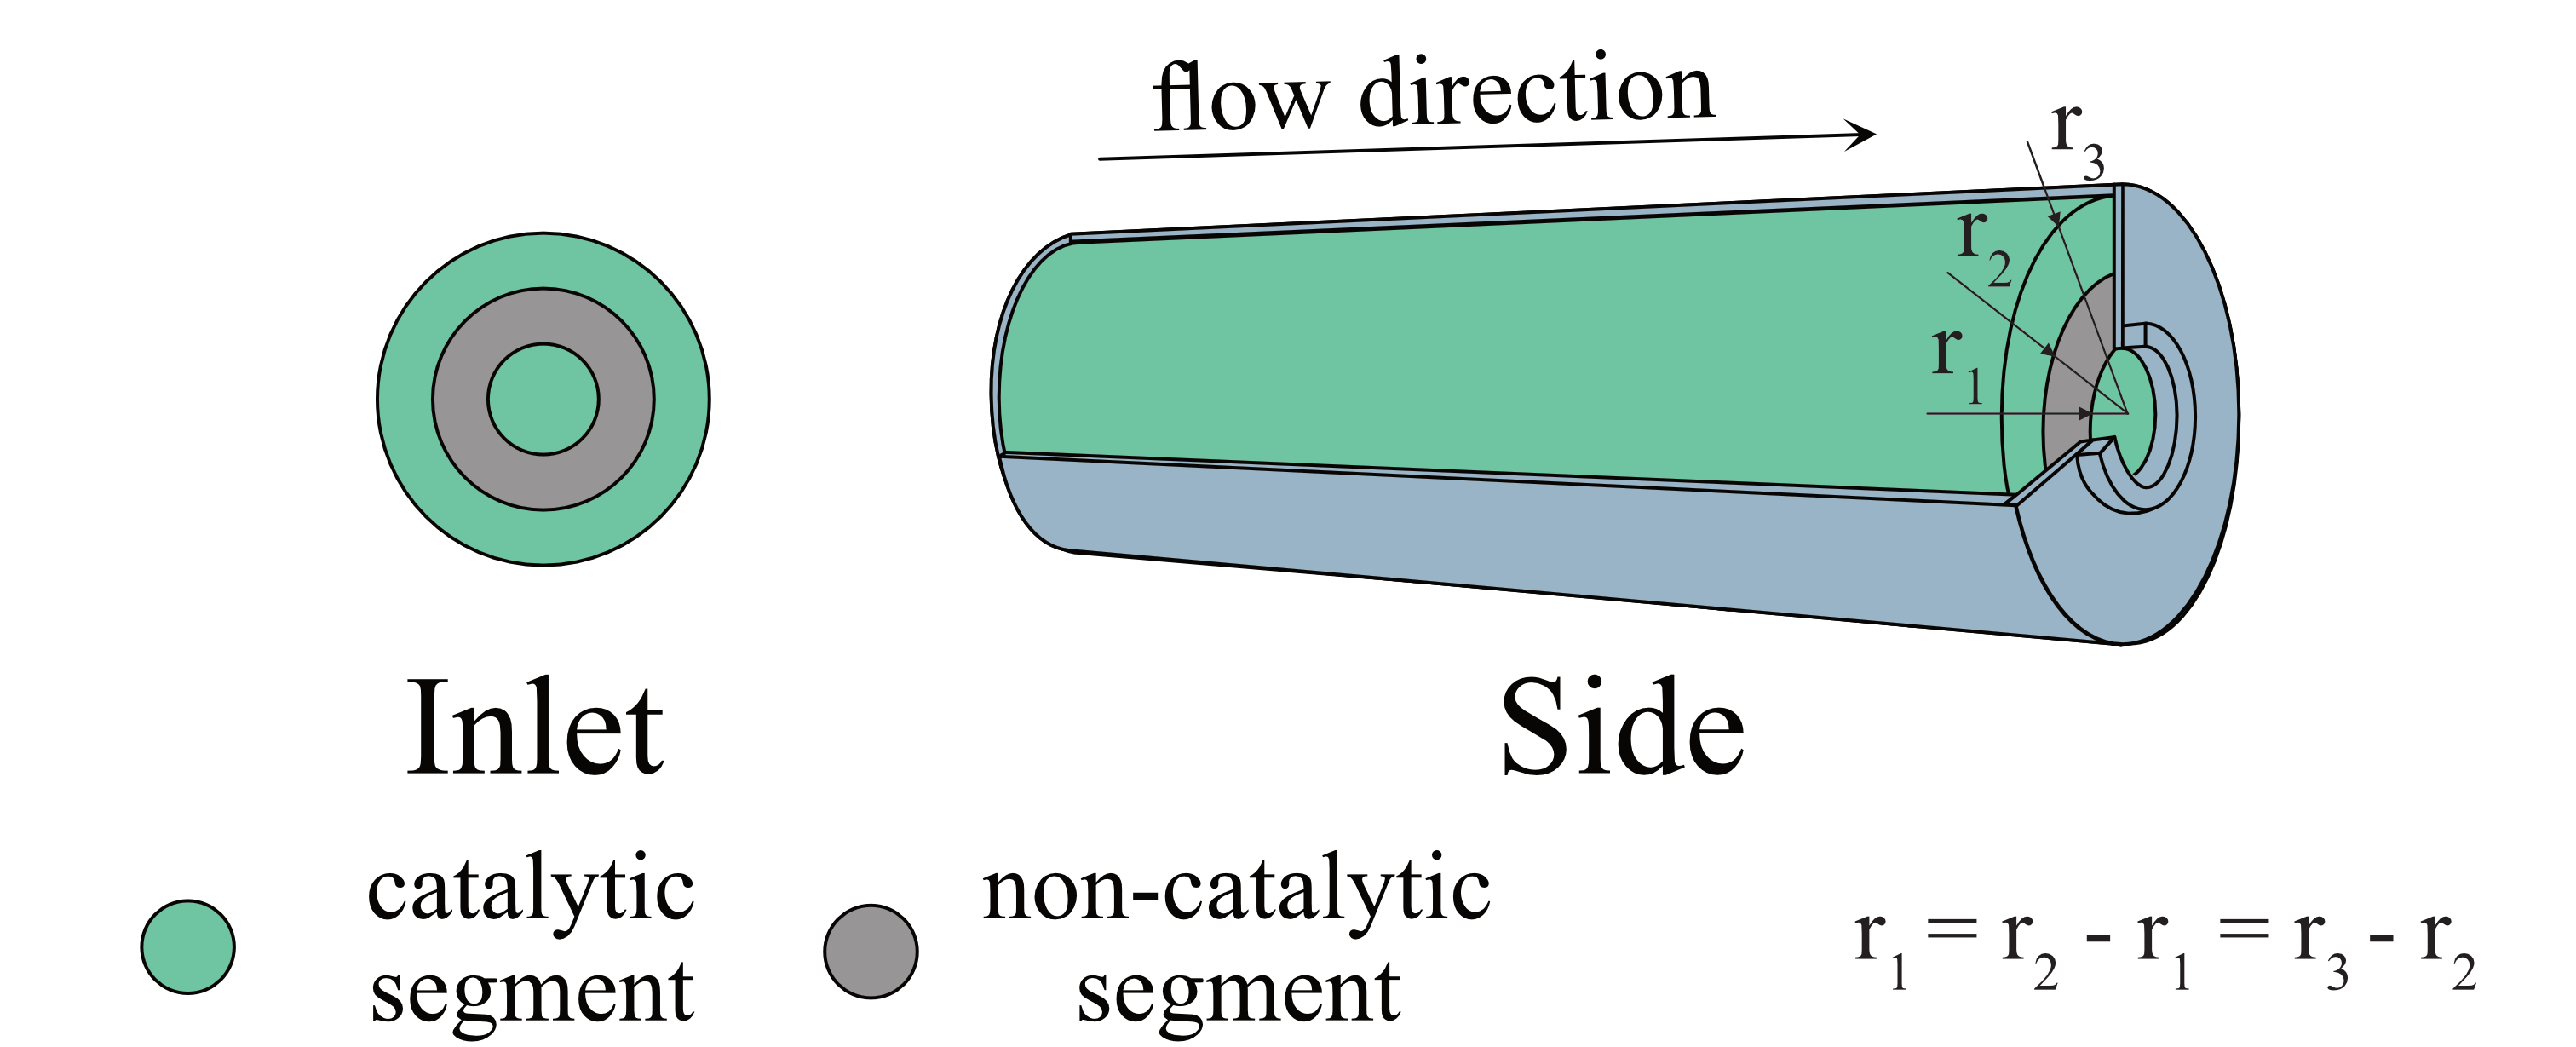
\includegraphics[width=120mm]{5seg.png}
%\caption{\label{fig:5seg}Catalytic insert division strategy I}
%\end{figure}
%
%
%\paragraph{Thermal fitness 80 \%, methane conversion 20 \%} \hspace{0pt} \\
%\noindent 
%
%\begin{figure}[h!]
%\centering
%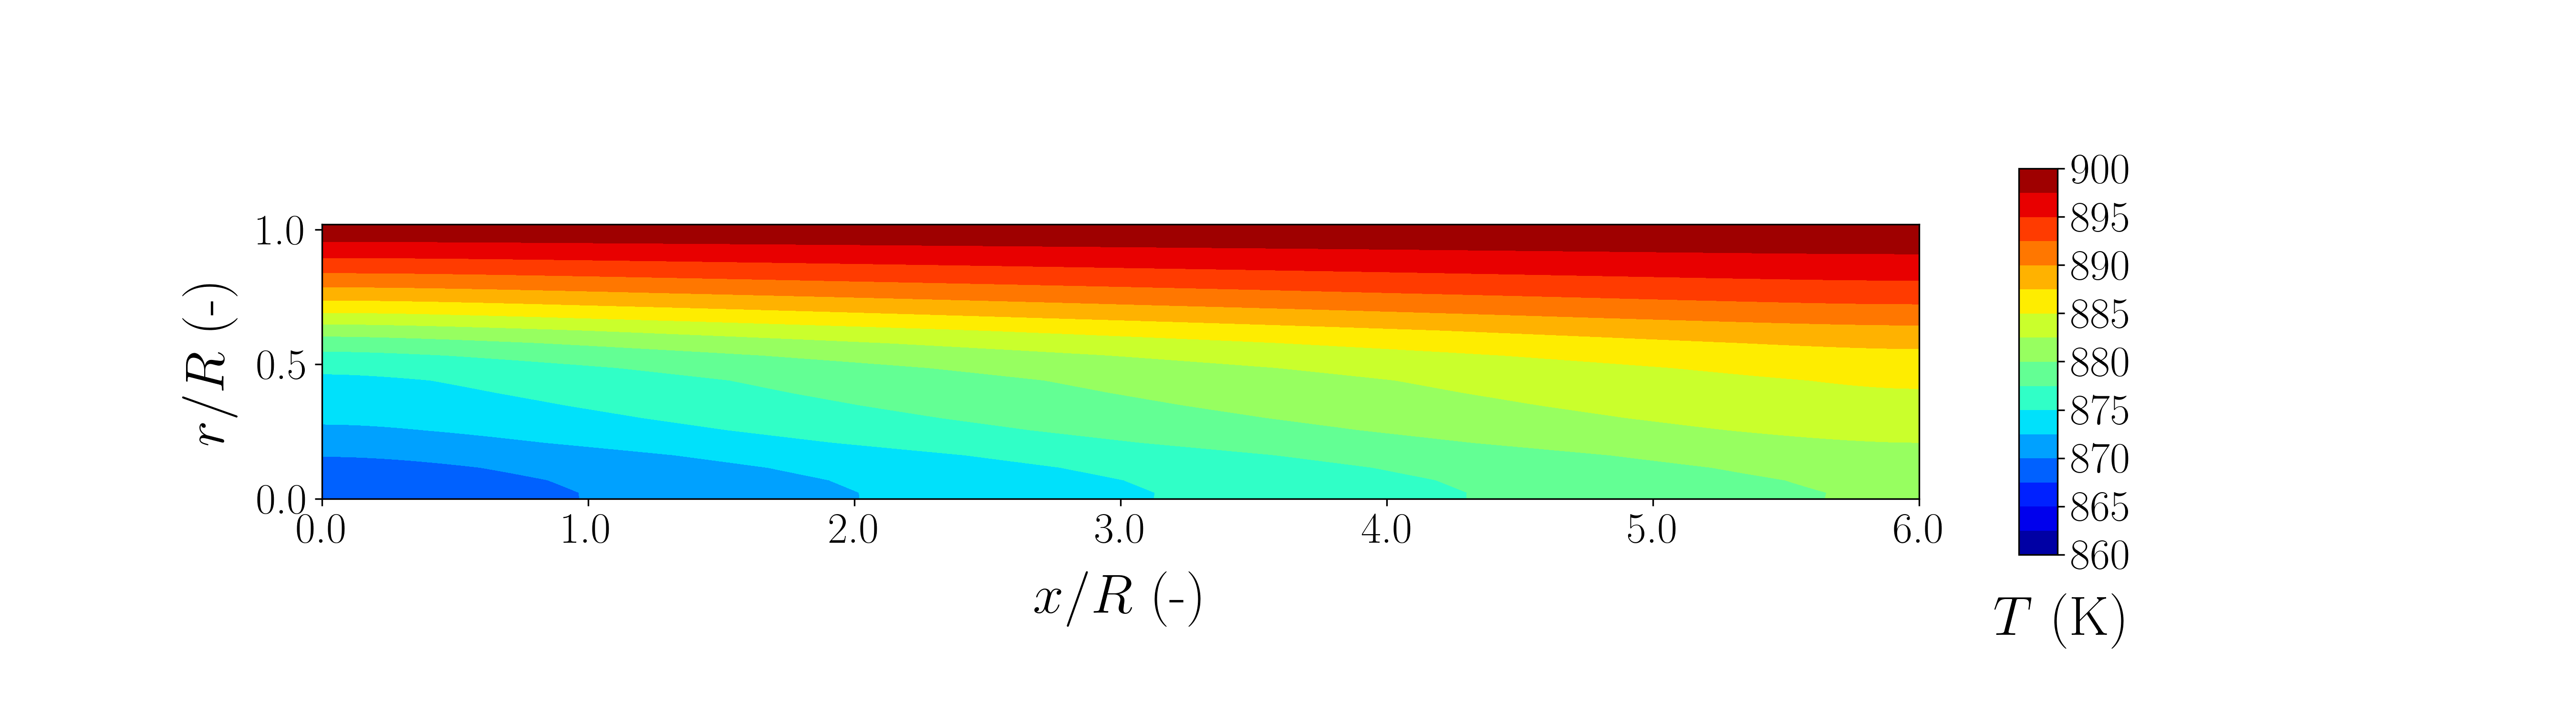
\includegraphics[width=190mm]{results/5/20C_80T/GEN1-TFIELD.png}
%\caption{\label{fig:5R2080G1-TField} Strategy I - Temperature field distribution - 1$^{\rm{st}}$ generation ($w_{\rm{CH_4}} = 0.2, w_T = 0.8$, $T_{\rm{in}}$ = 900 K, $u_{\rm{in}}$ = 0.15 m s$^{-1}$, $SC$ = 2.0)}
%\end{figure}
%
%\begin{figure}[h!]
%\centering
%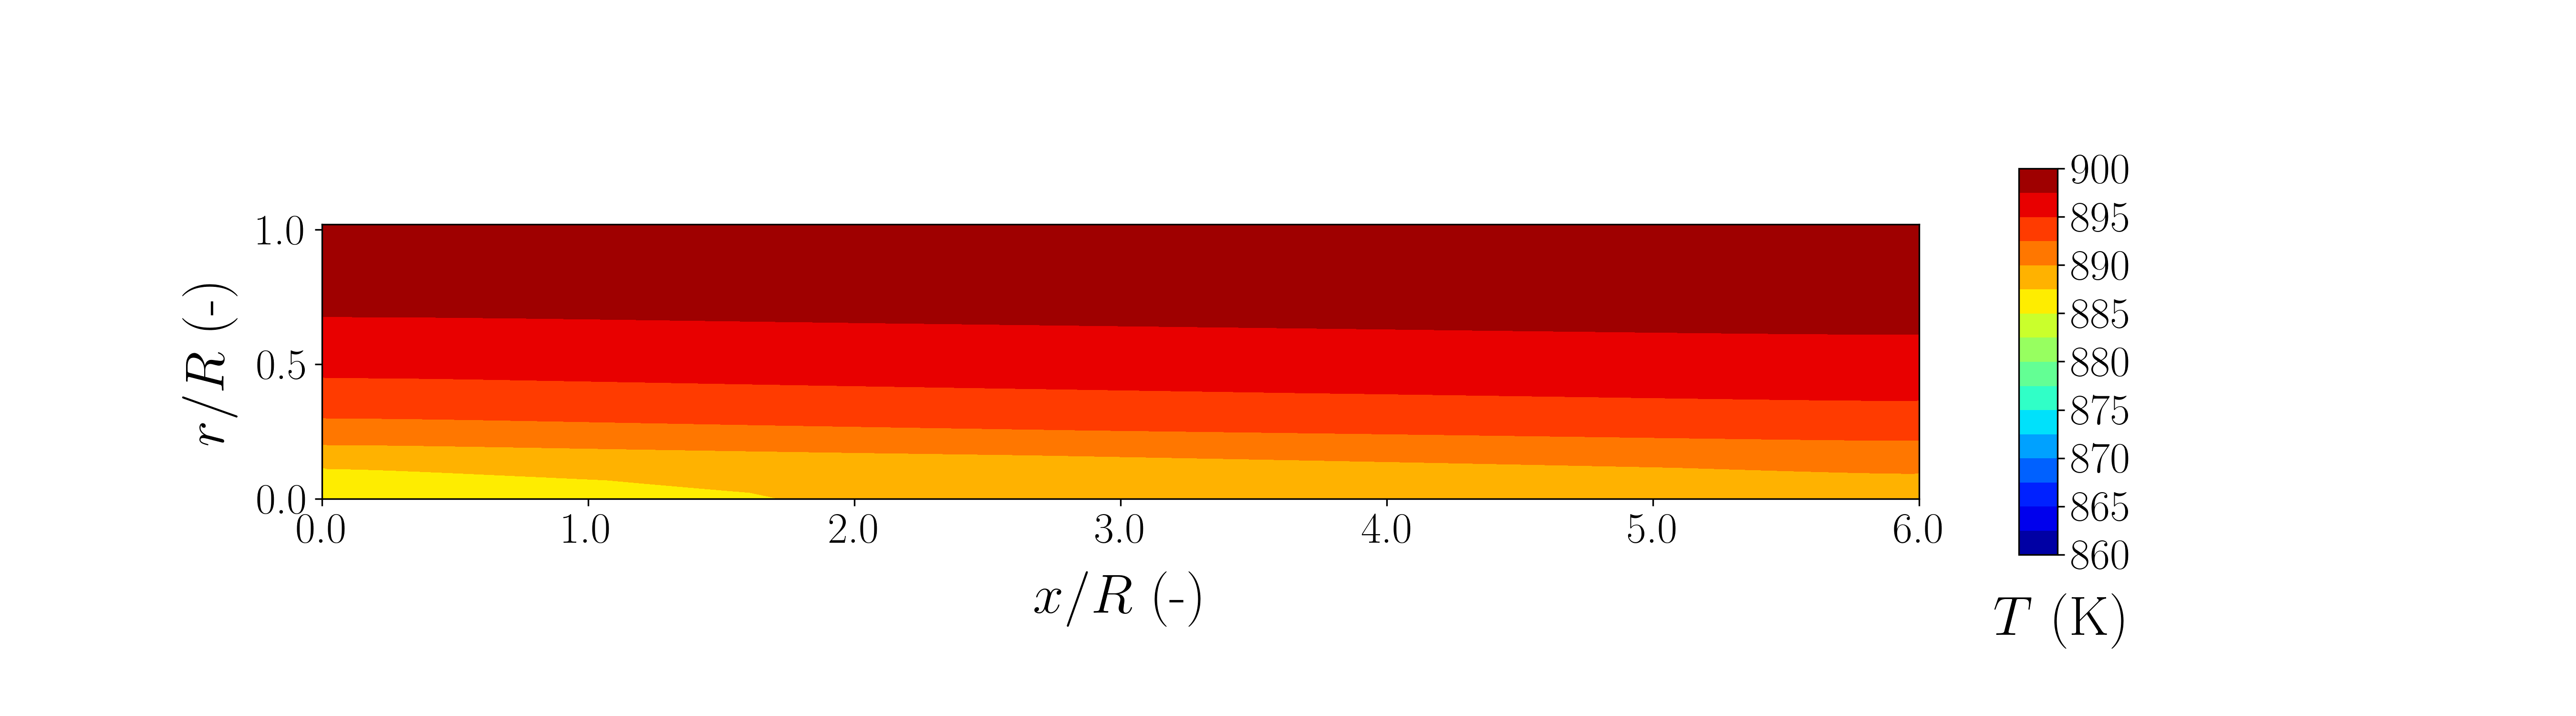
\includegraphics[width=190mm]{results/5/20C_80T/GEN15-TFIELD.png}
%\caption{\label{fig:5R2080G15-TField} Strategy I - Temperature field distribution - 15$^{\rm{th}}$ generation ($w_{\rm{CH_4}} = 0.2, w_T = 0.8$, $T_{\rm{in}}$ = 900 K, $u_{\rm{in}}$ = 0.15 m s$^{-1}$, $SC$ = 2.0)}
%\end{figure}
%
%\begin{figure}[h!]
%\centering
%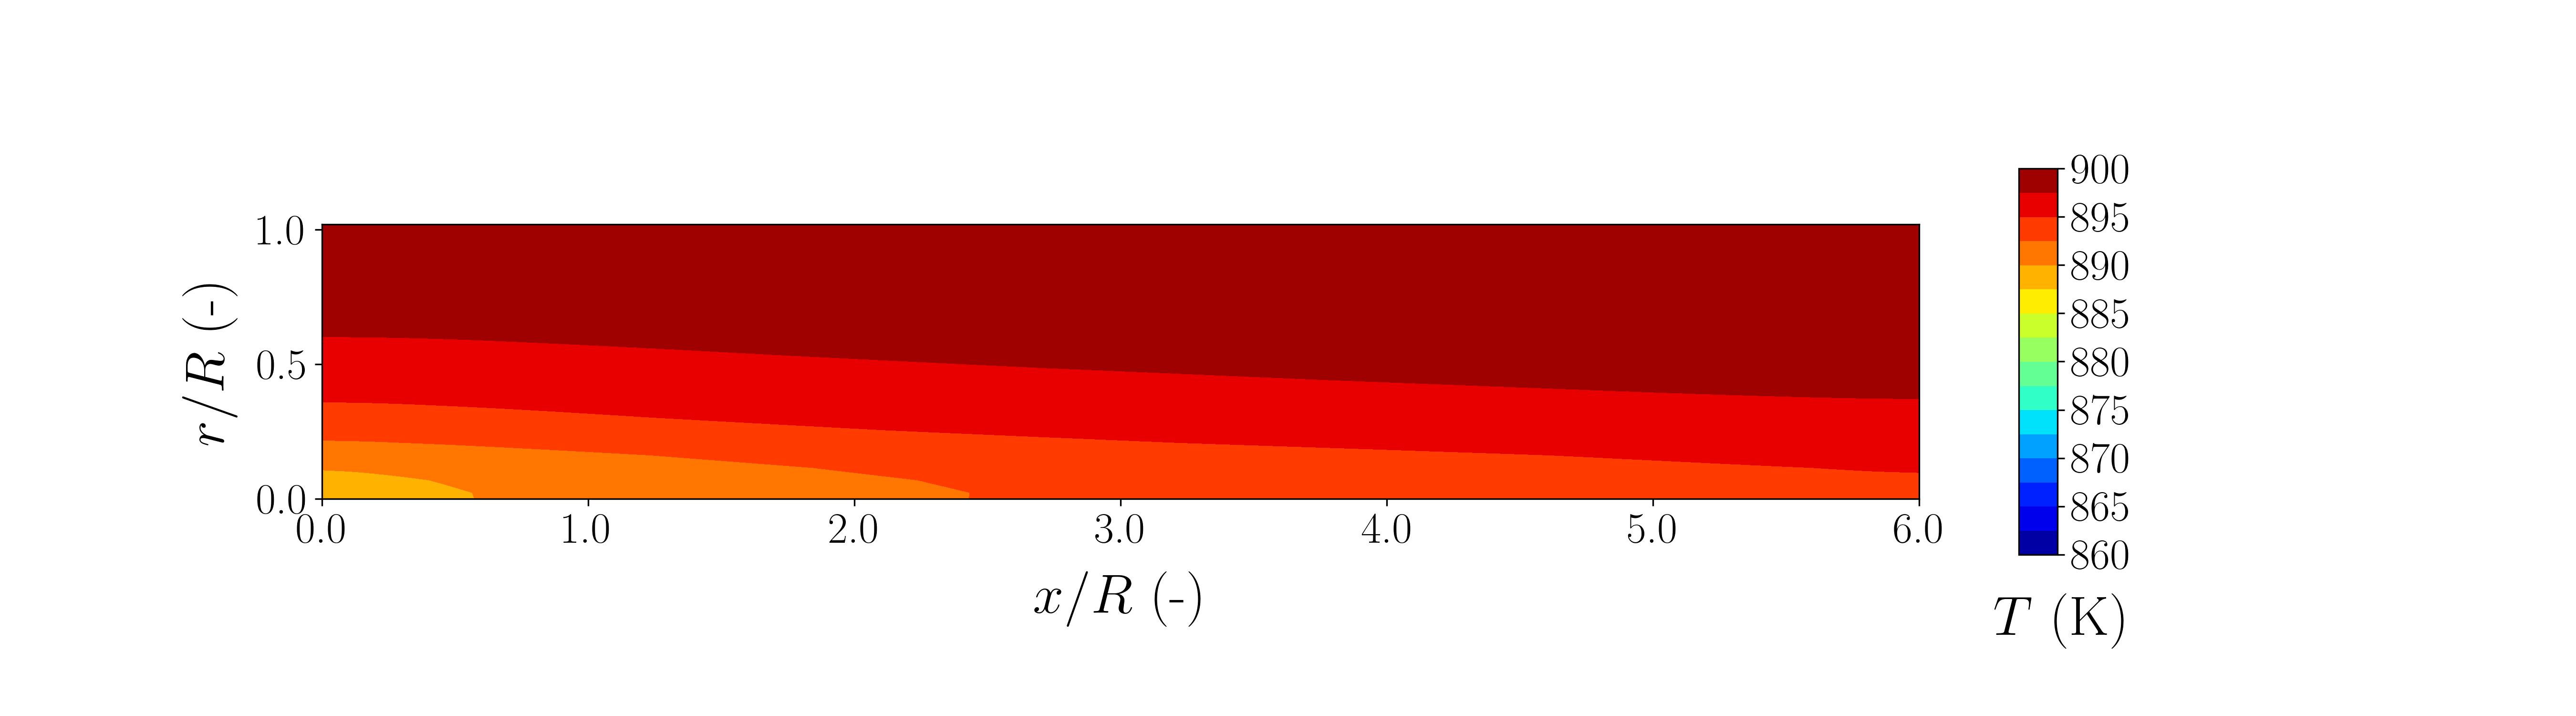
\includegraphics[width=190mm]{results/5/20C_80T/GEN30-TFIELD.png}
%\caption{\label{fig:5R2080G30-TField} Strategy I - Temperature field distribution - 30$^{\rm{th}}$ generation ($w_{\rm{CH_4}} = 0.2, w_T = 0.8$, $T_{\rm{in}}$ = 900 K, $u_{\rm{in}}$ = 0.15 m s$^{-1}$, $SC$ = 2.0)}
%\end{figure}
%
%
%\begin{figure}[h!]
%\centering
%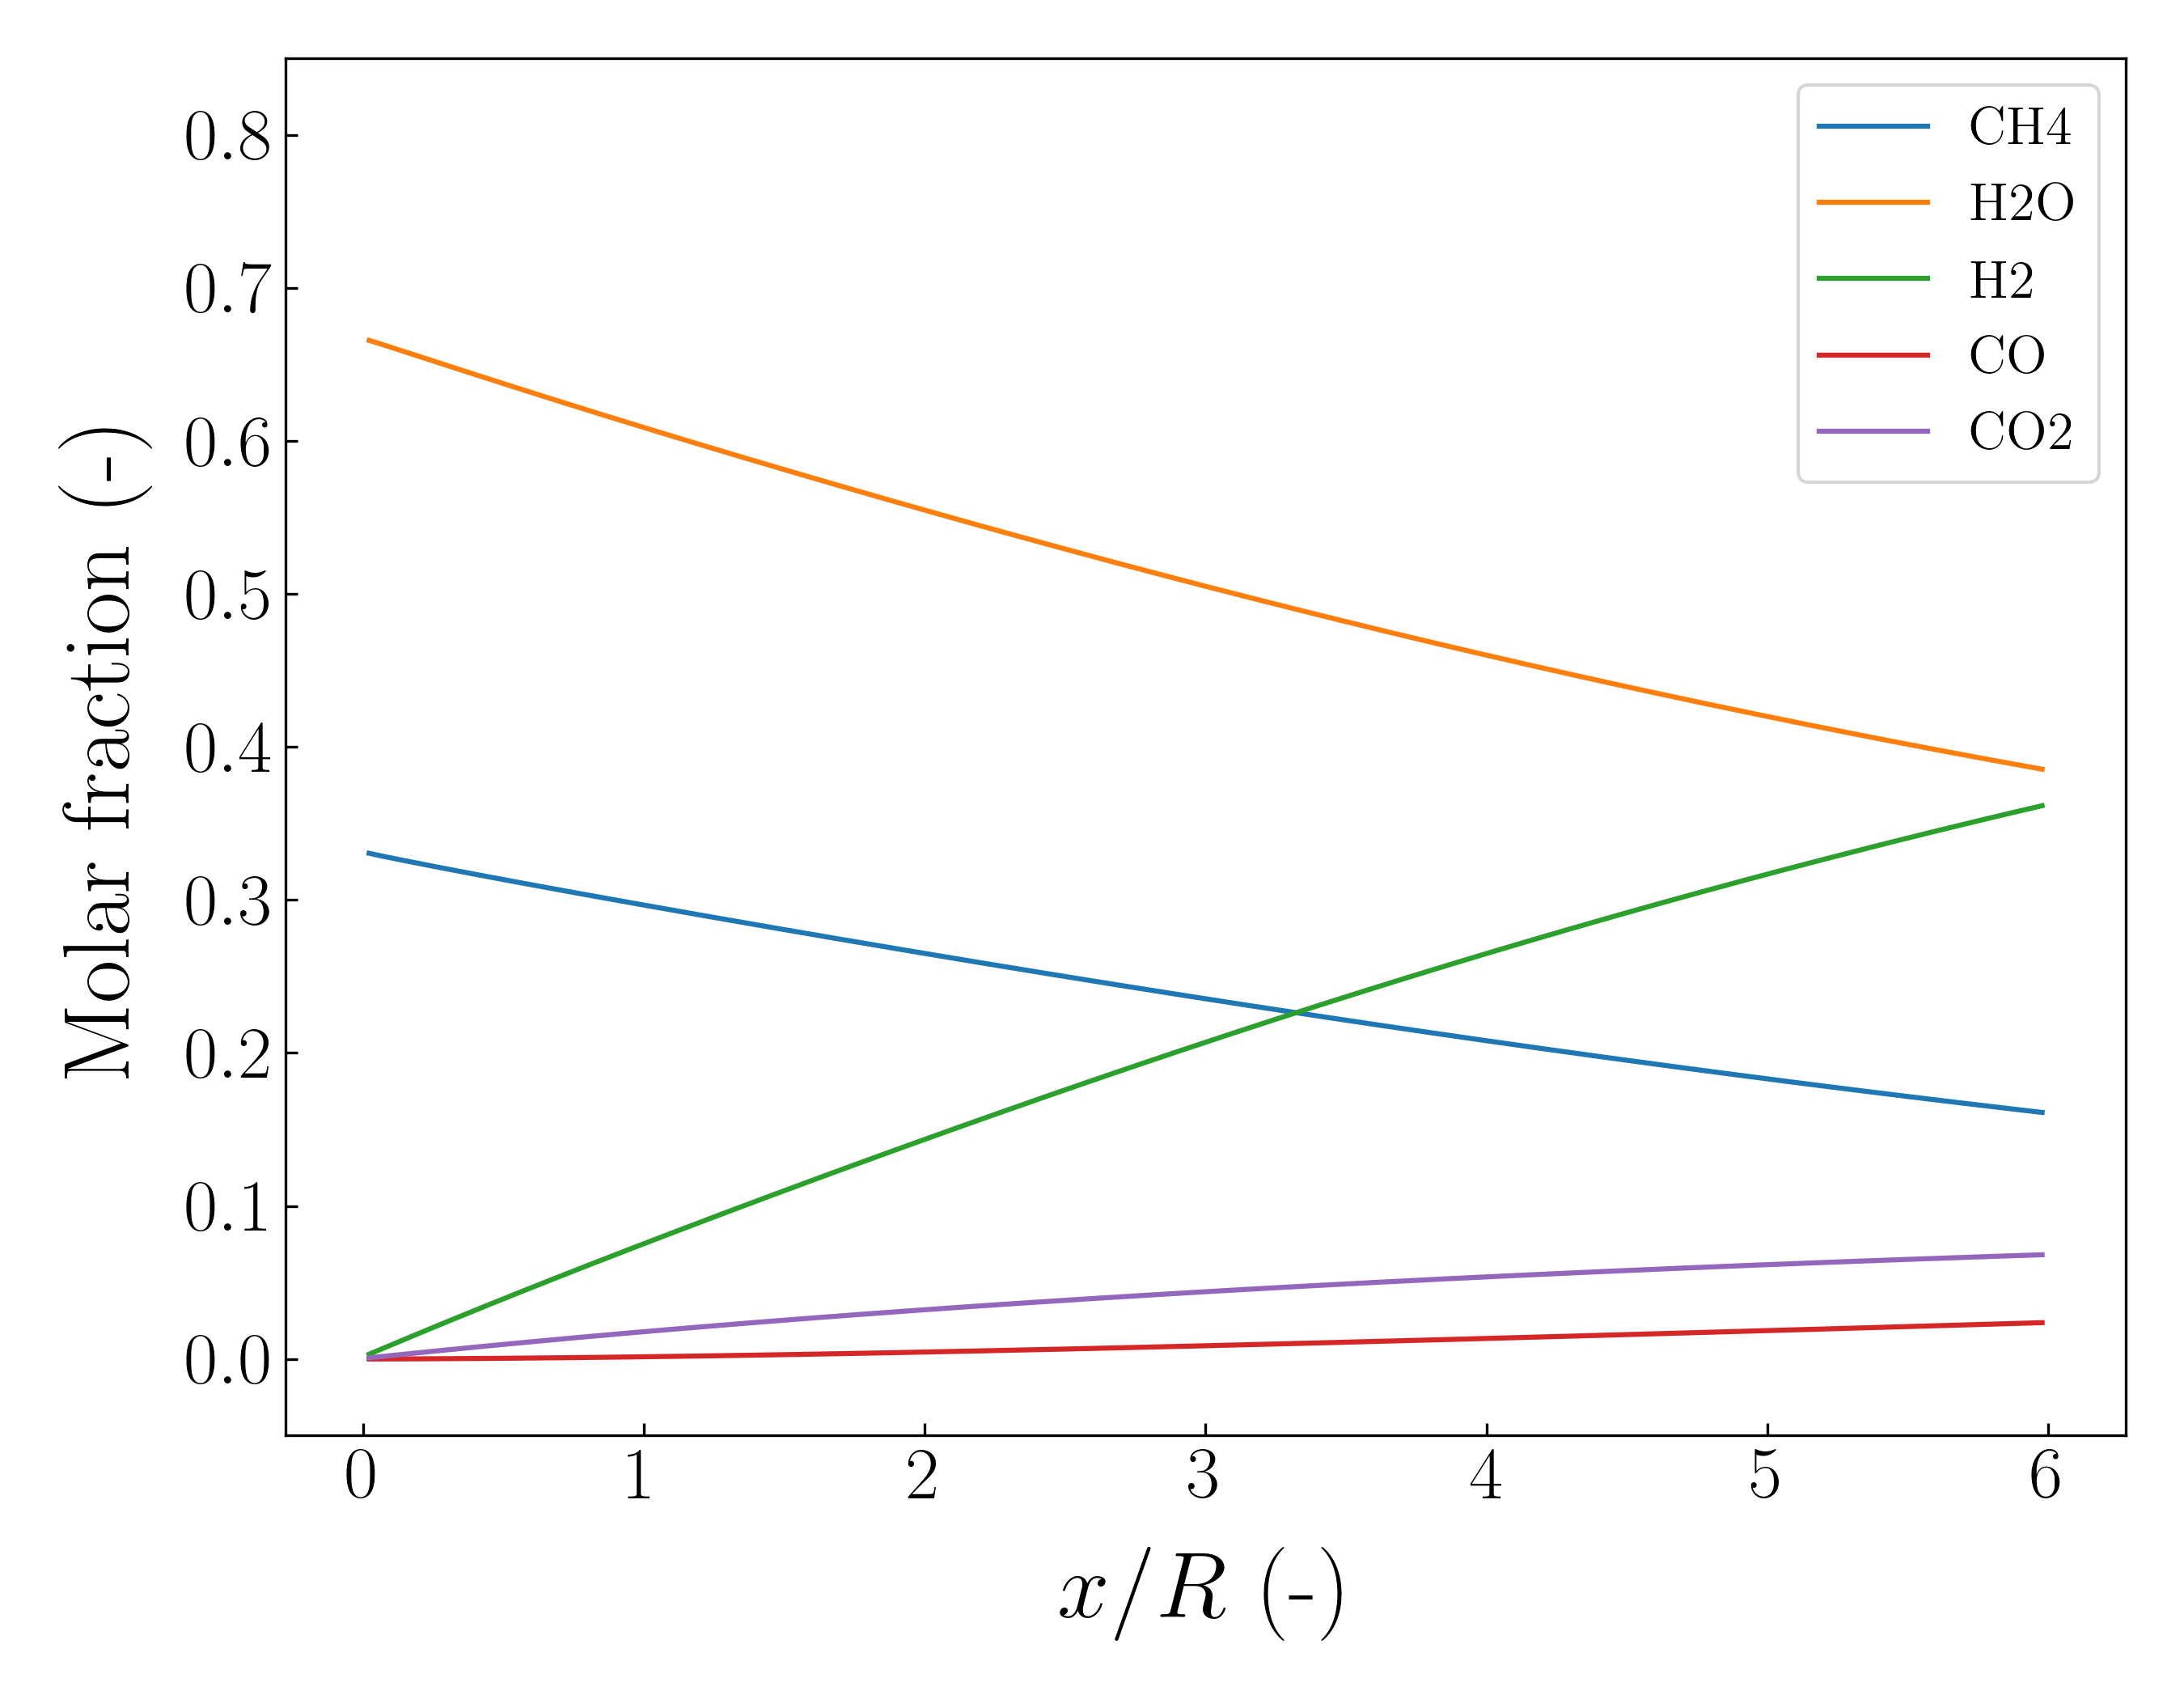
\includegraphics[width=80mm]{results/5/20C_80T/GEN1-AVG.png}
%\caption{\label{fig:5R2080G1-avg} Strategy I - Radius-averaged molar fractions - 1$^{\rm{st}}$ generation ($w_{\rm{CH_4}} = 0.2, w_T = 0.8$, $T_{\rm{in}}$ = 900 K, $u_{\rm{in}}$ = 0.15 m s$^{-1}$, $SC$ = 2.0)}
%\end{figure}
%
%\begin{figure}[h!]
%\centering
%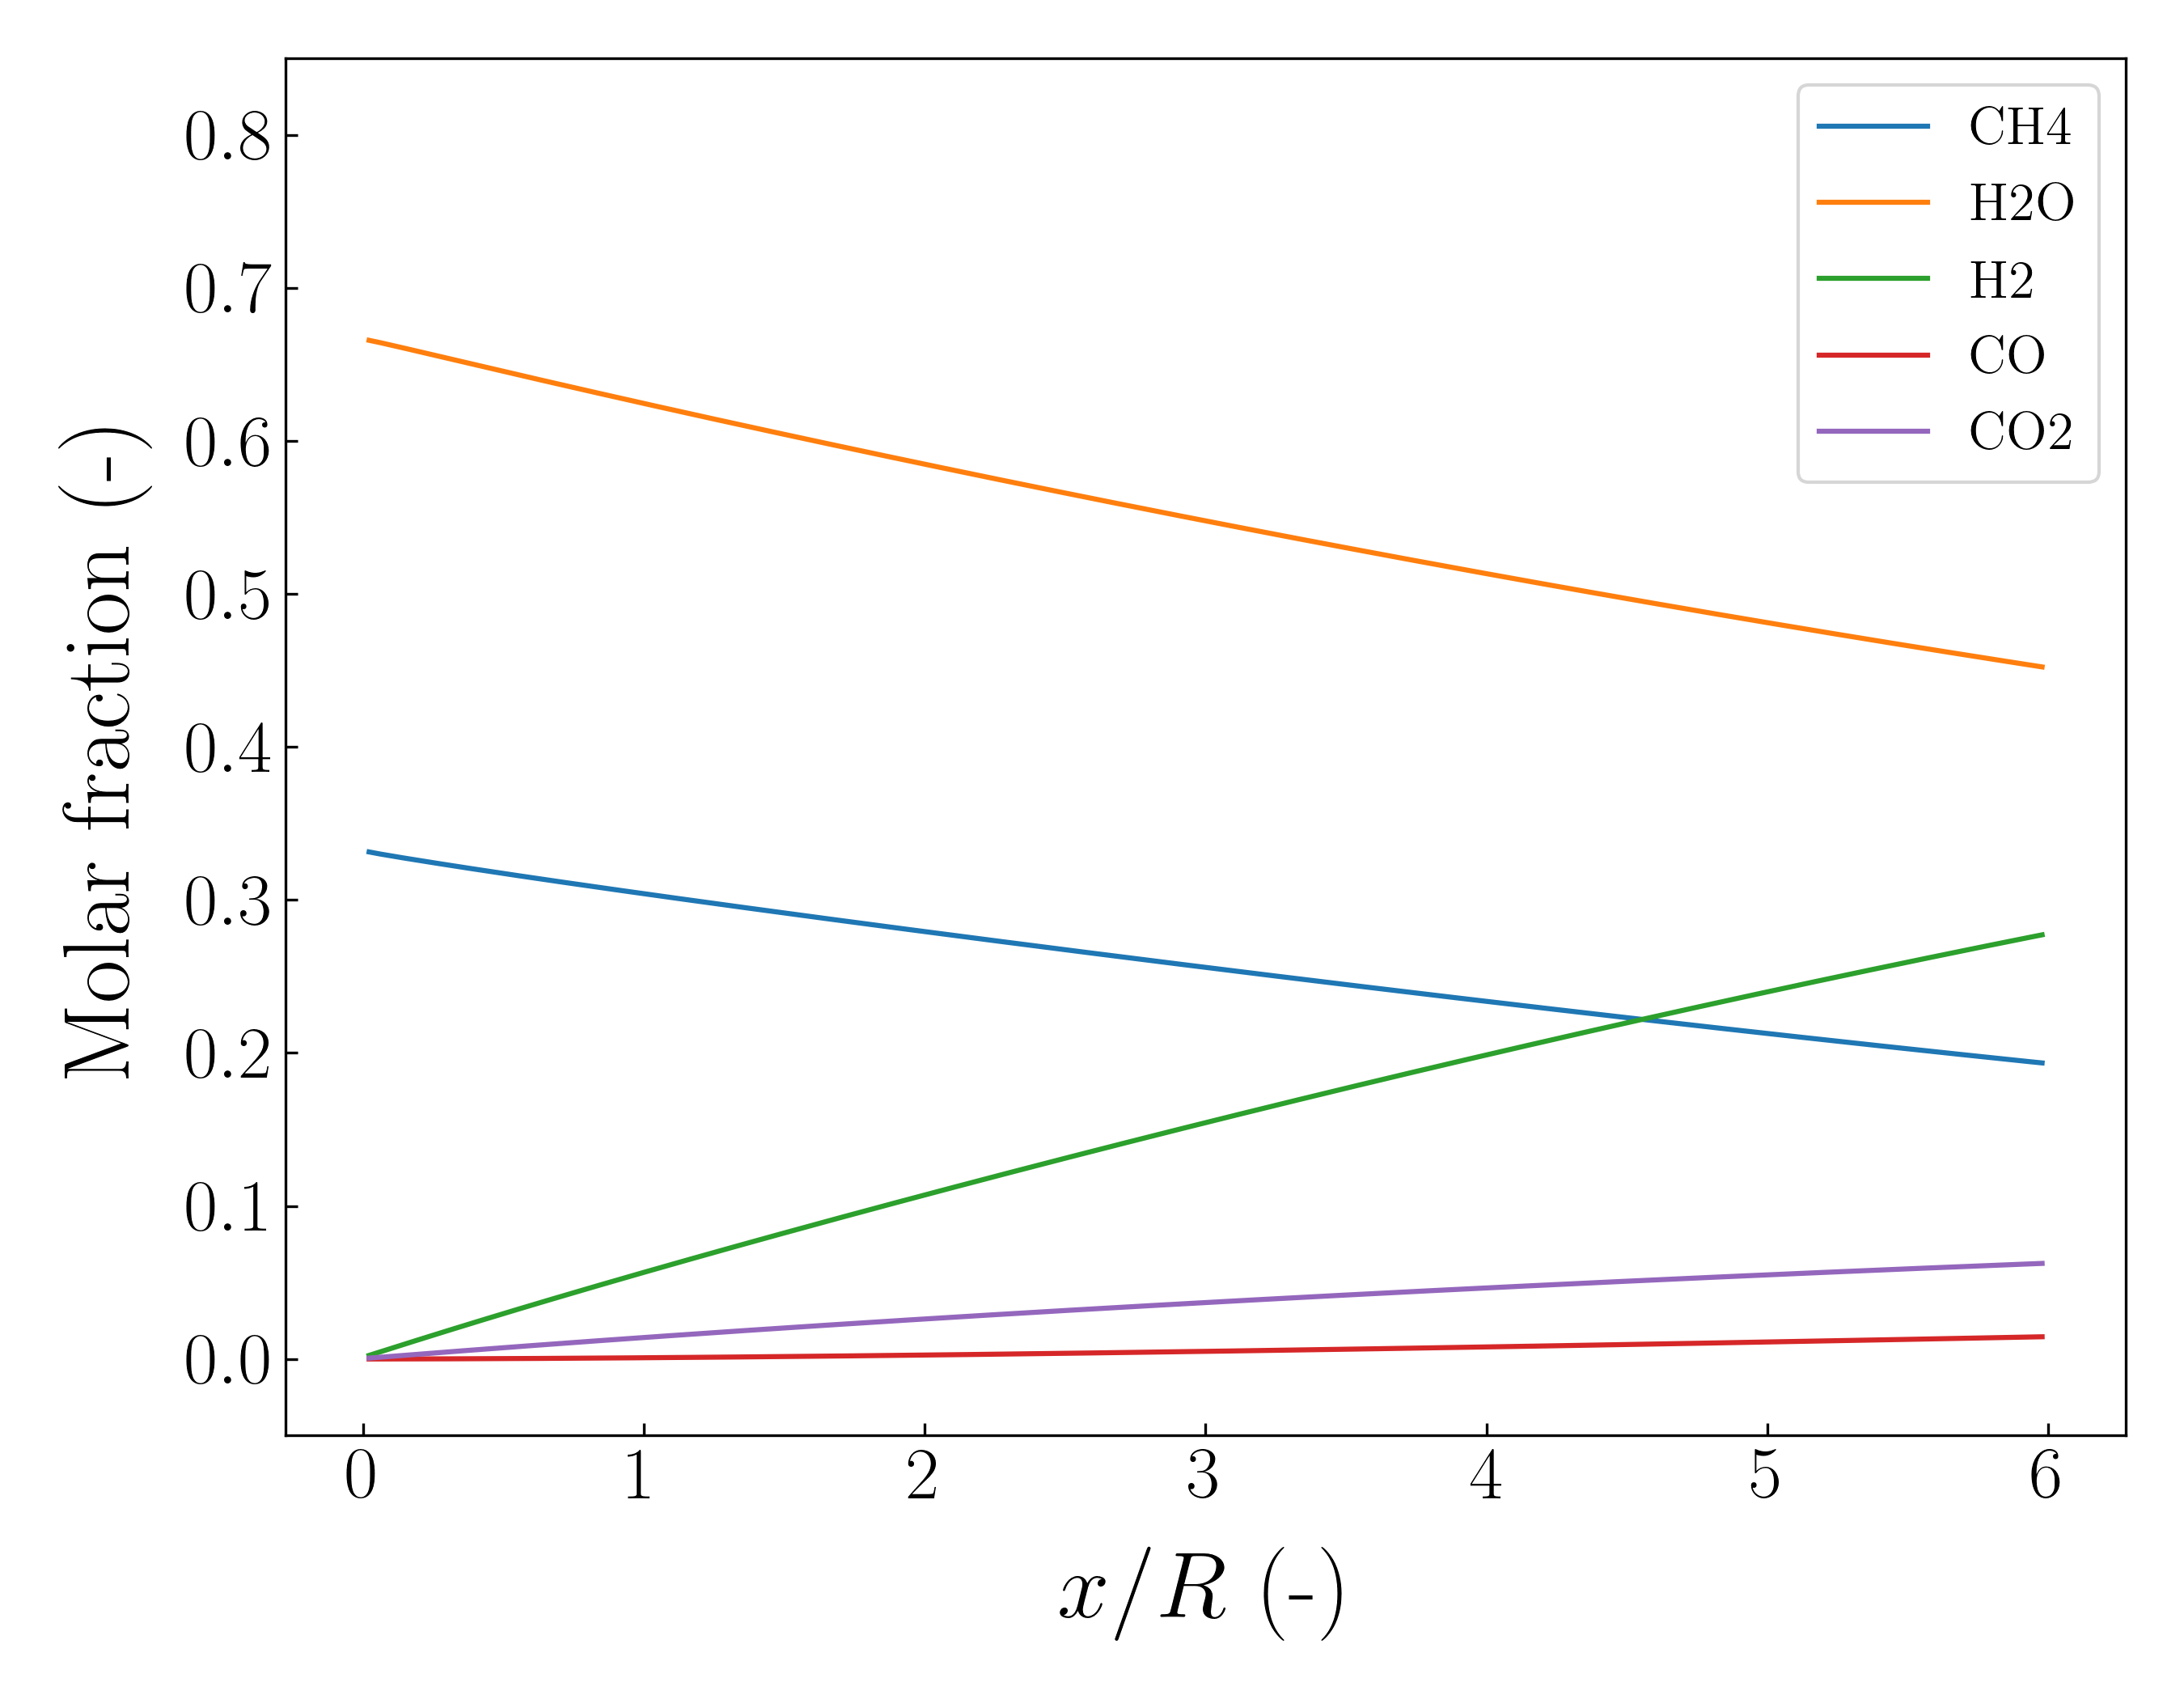
\includegraphics[width=80mm]{results/5/20C_80T/GEN15-AVG.png}
%\caption{\label{fig:5R2080G15-avg} Strategy I - Radius-averaged molar fractions - 15$^{\rm{th}}$ generation ($w_{\rm{CH_4}} = 0.2, w_T = 0.8$, $T_{\rm{in}}$ = 900 K, $u_{\rm{in}}$ = 0.15 m s$^{-1}$, $SC$ = 2.0)}
%\end{figure}
%
%\begin{figure}[h!]
%\centering
%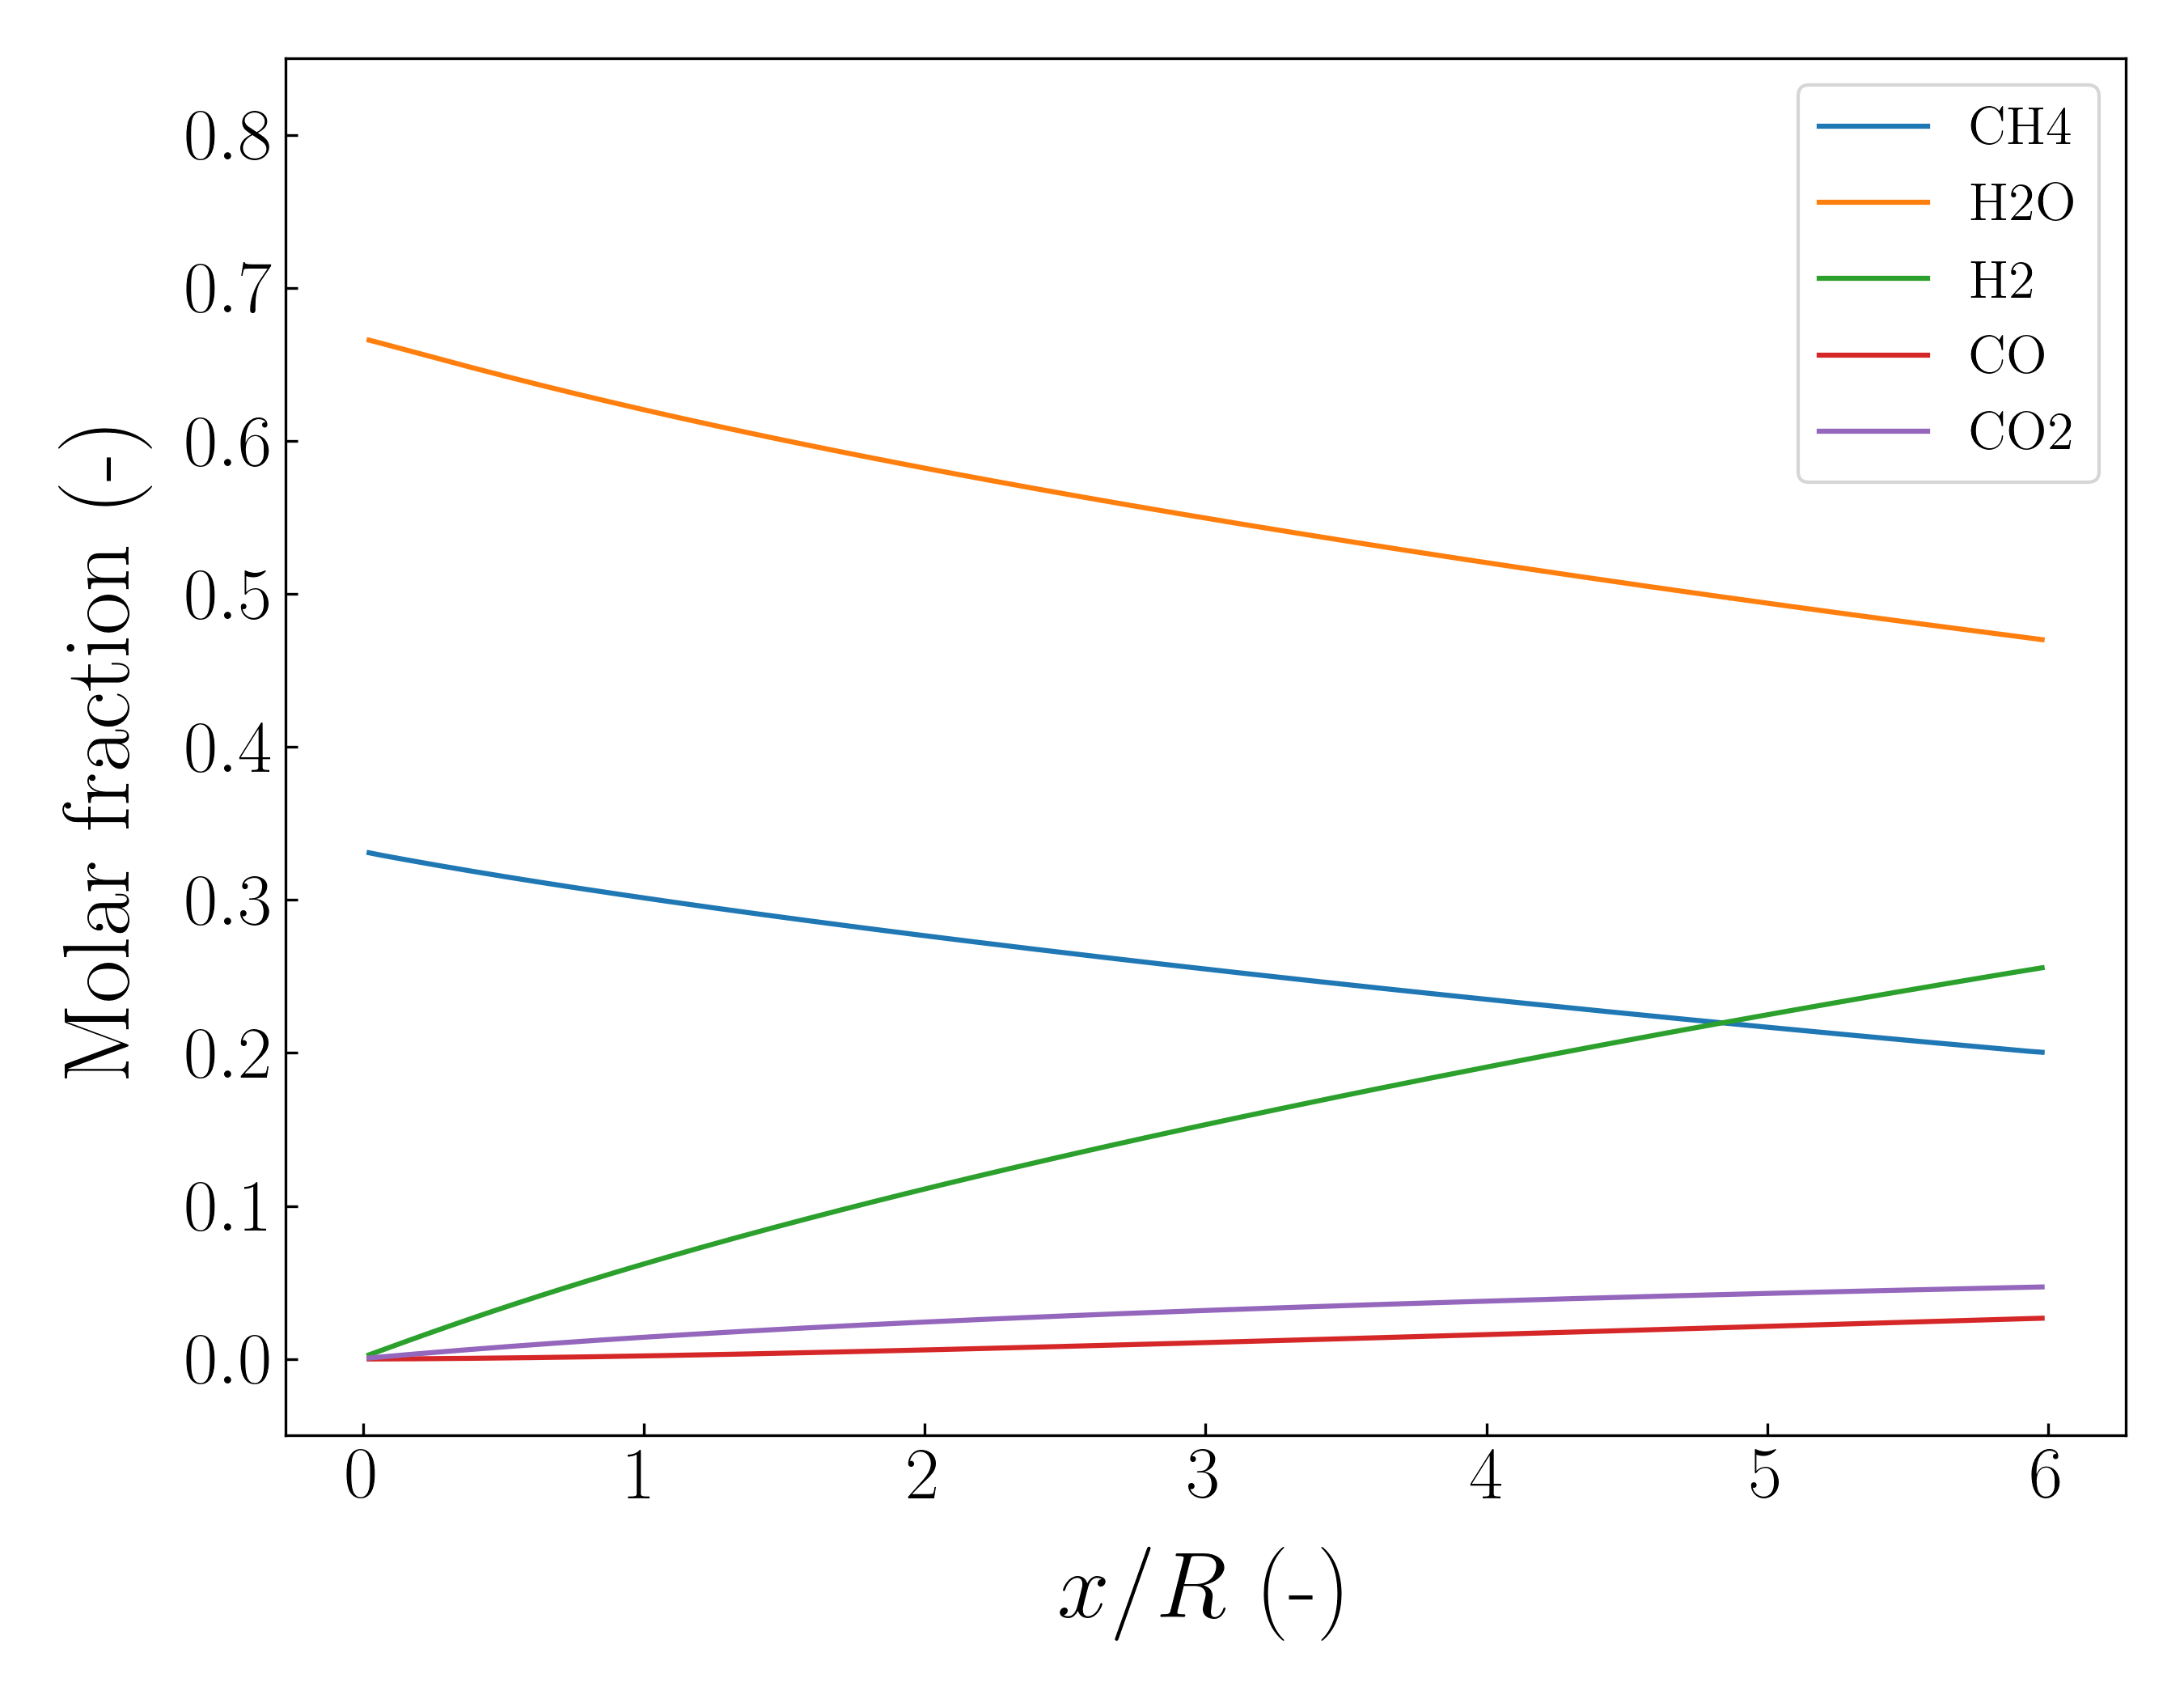
\includegraphics[width=80mm]{results/5/20C_80T/GEN30-AVG.png}
%\caption{\label{fig:5R2080G30-avg} Strategy I - Radius-averaged molar fractions -  30$^{\rm{th}}$ generation ($w_{\rm{CH_4}} = 0.2, w_T = 0.8$, $T_{\rm{in}}$ = 900 K, $u_{\rm{in}}$ = 0.15 m s$^{-1}$, $SC$ = 2.0)}
%\end{figure}
%
%\begin{figure}[h!]
%\centering
%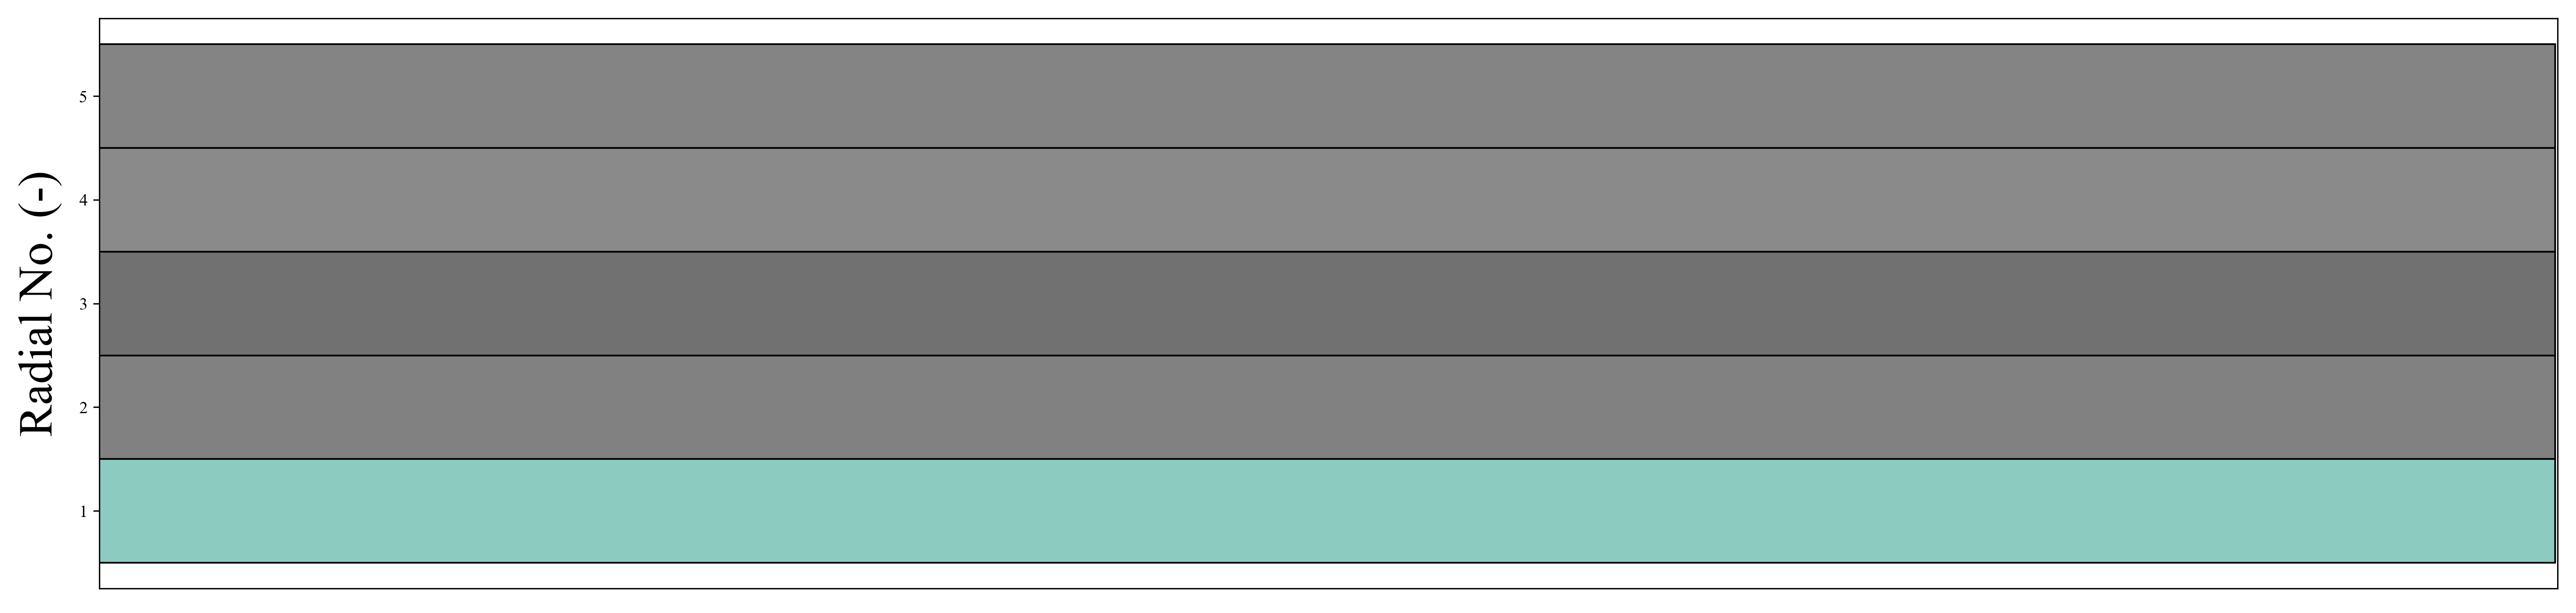
\includegraphics[width=120mm]{results/segments/5seg/20C80T/seg.png}
%\caption{\label{fig:30L6040G1-TField} Strategy I - Segments distribution for 30$^{\rm{th}}$ generation ($w_{\rm{CH_4}} = 0.2, w_T = 0.8$, $T_{\rm{in}}$ = 900 K, $u_{\rm{in}}$ = 0.15 m s$^{-1}$, $SC$ = 2.0)}
%\end{figure}
%
%\begin{figure}[h!]
%\centering
%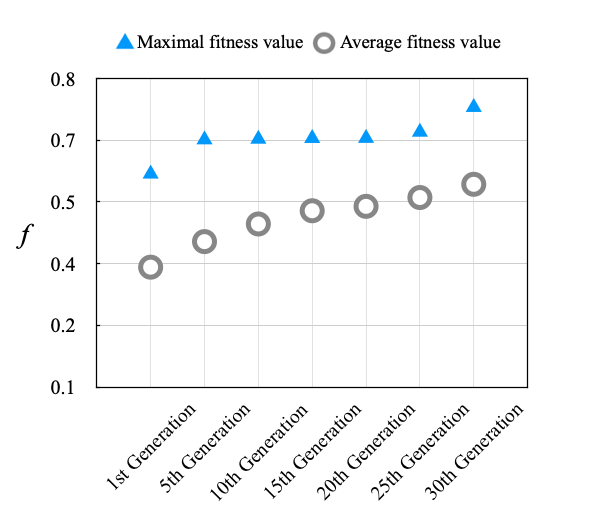
\includegraphics[width=100mm]{results/5/20C_80T.png}
%\caption{\label{fig:5R2080G-fitness} Strategy I - Fitness analysis throughout successive populations ($w_{\rm{CH_4}} = 0.2, w_T = 0.8$, $T_{\rm{in}}$ = 900 K, $u_{\rm{in}}$ = 0.15 m s$^{-1}$, $SC$ = 2.0)}
%\end{figure}
%
%
%
%\clearpage
%
%
%
%\paragraph{Thermal fitness 60 \%, methane conversion 40 \%} \hspace{0pt} \\
%\noindent 
%
%
%\begin{figure}[h!]
%\centering
%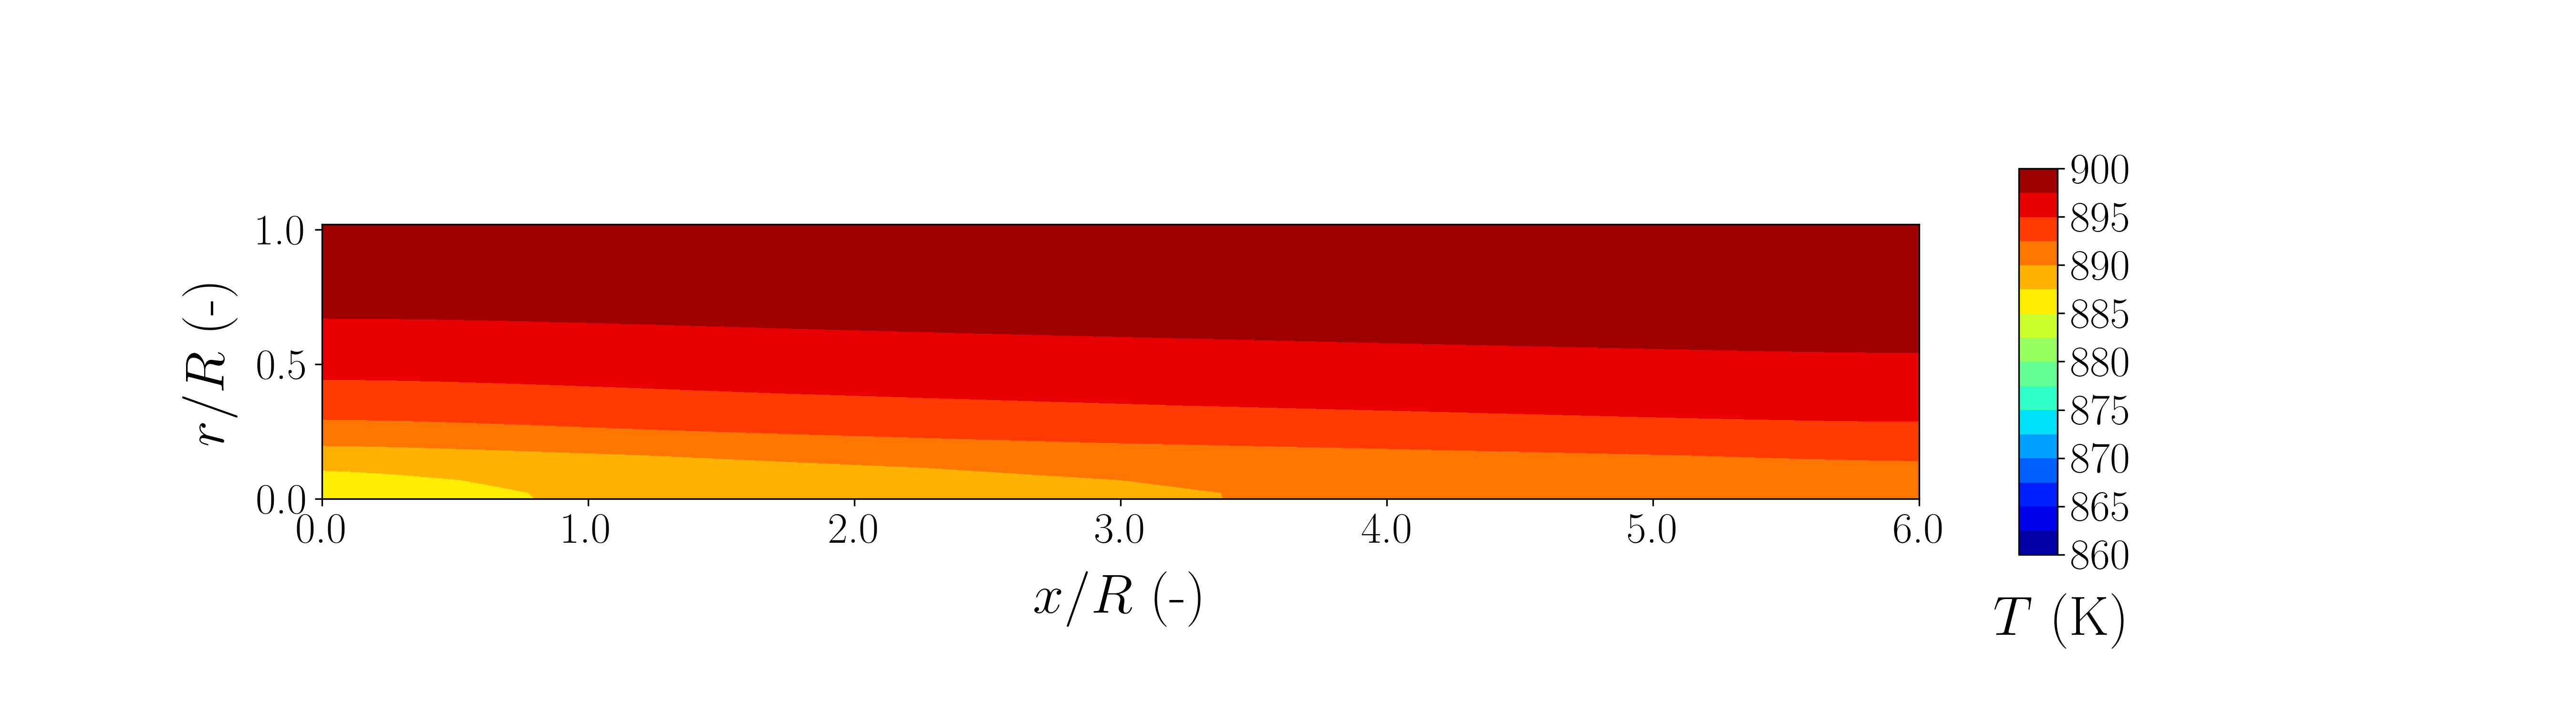
\includegraphics[width=190mm]{results/5/40C_60T/GEN1-TFIELD.png}
%\caption{\label{fig:5R4060G1-TField} Strategy I - Temperature field distribution - 1$^{\rm{st}}$ generation ($w_{\rm{CH_4}} = 0.4, w_T = 0.6$, $T_{\rm{in}}$ = 900 K, $u_{\rm{in}}$ = 0.15 m s$^{-1}$, $SC$ = 2.0)}
%\end{figure}
%
%\begin{figure}[h!]
%\centering
%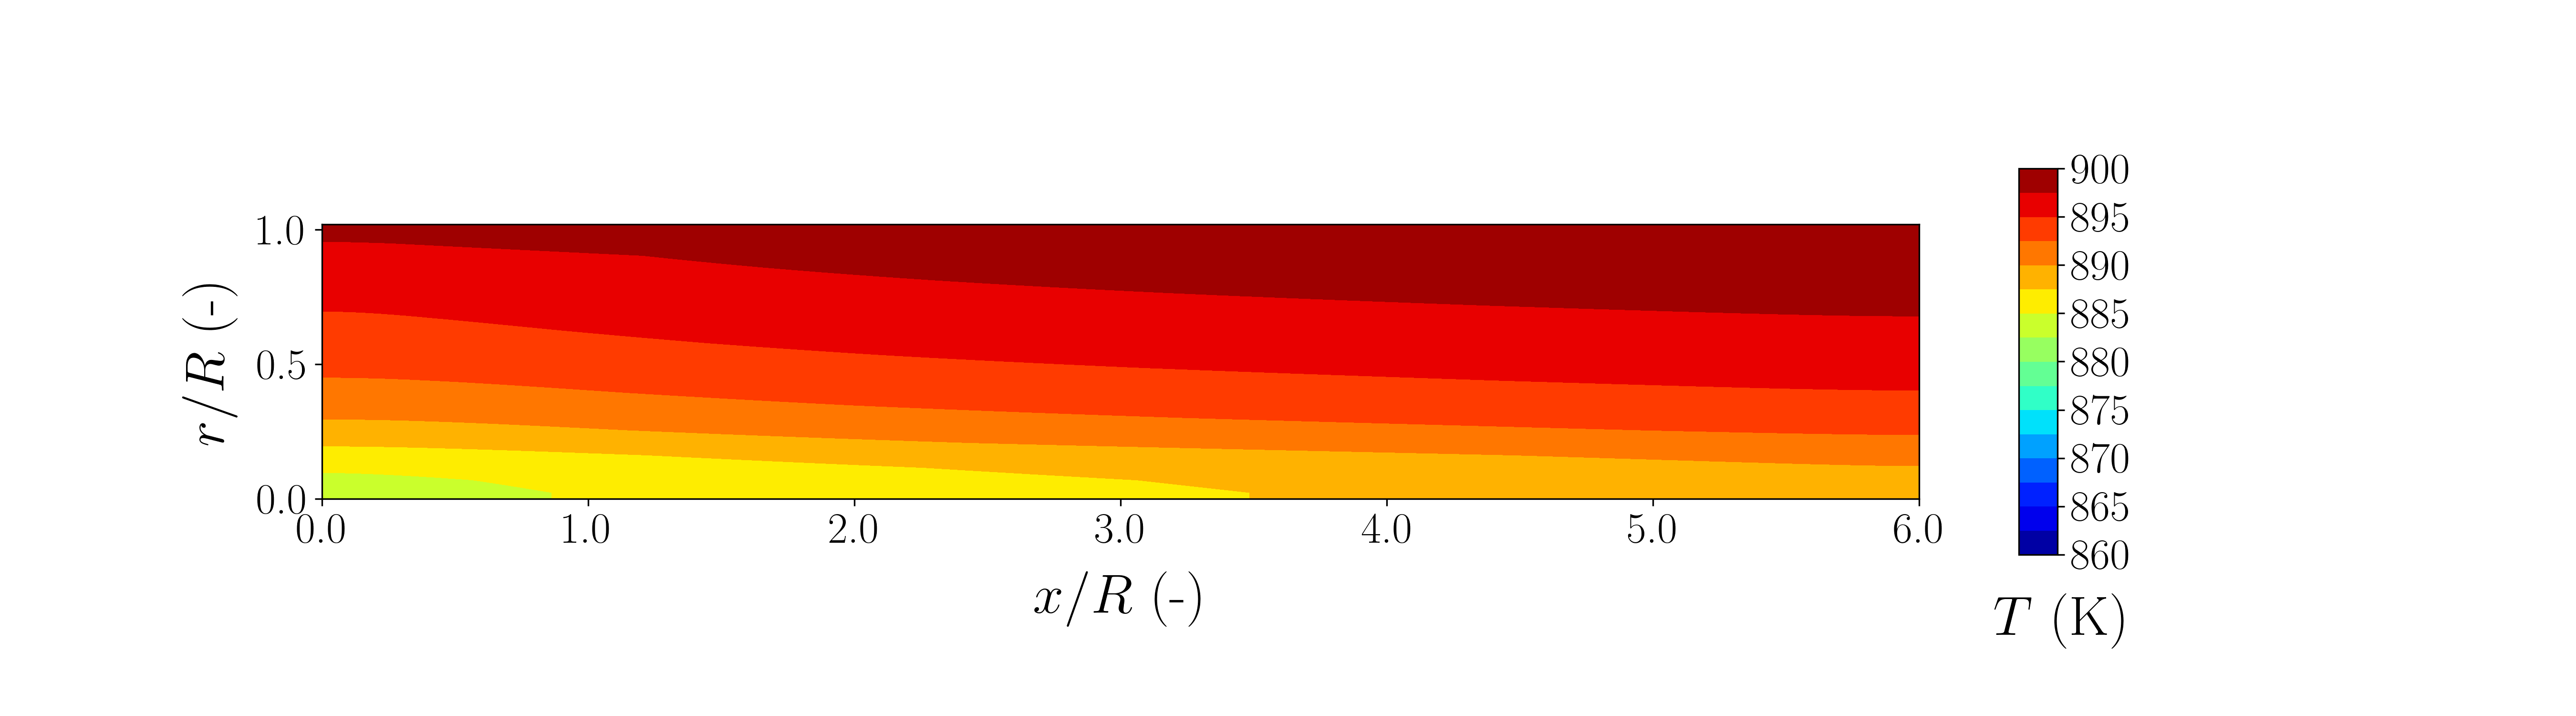
\includegraphics[width=190mm]{results/5/40C_60T/GEN15-TFIELD.png}
%\caption{\label{fig:5R4060G15-TField} Strategy I - Temperature field distribution - 15$^{\rm{th}}$ generation ($w_{\rm{CH_4}} = 0.4, w_T = 0.6$, $T_{\rm{in}}$ = 900 K, $u_{\rm{in}}$ = 0.15 m s$^{-1}$, $SC$ = 2.0)}
%\end{figure}
%
%\begin{figure}[h!]
%\centering
%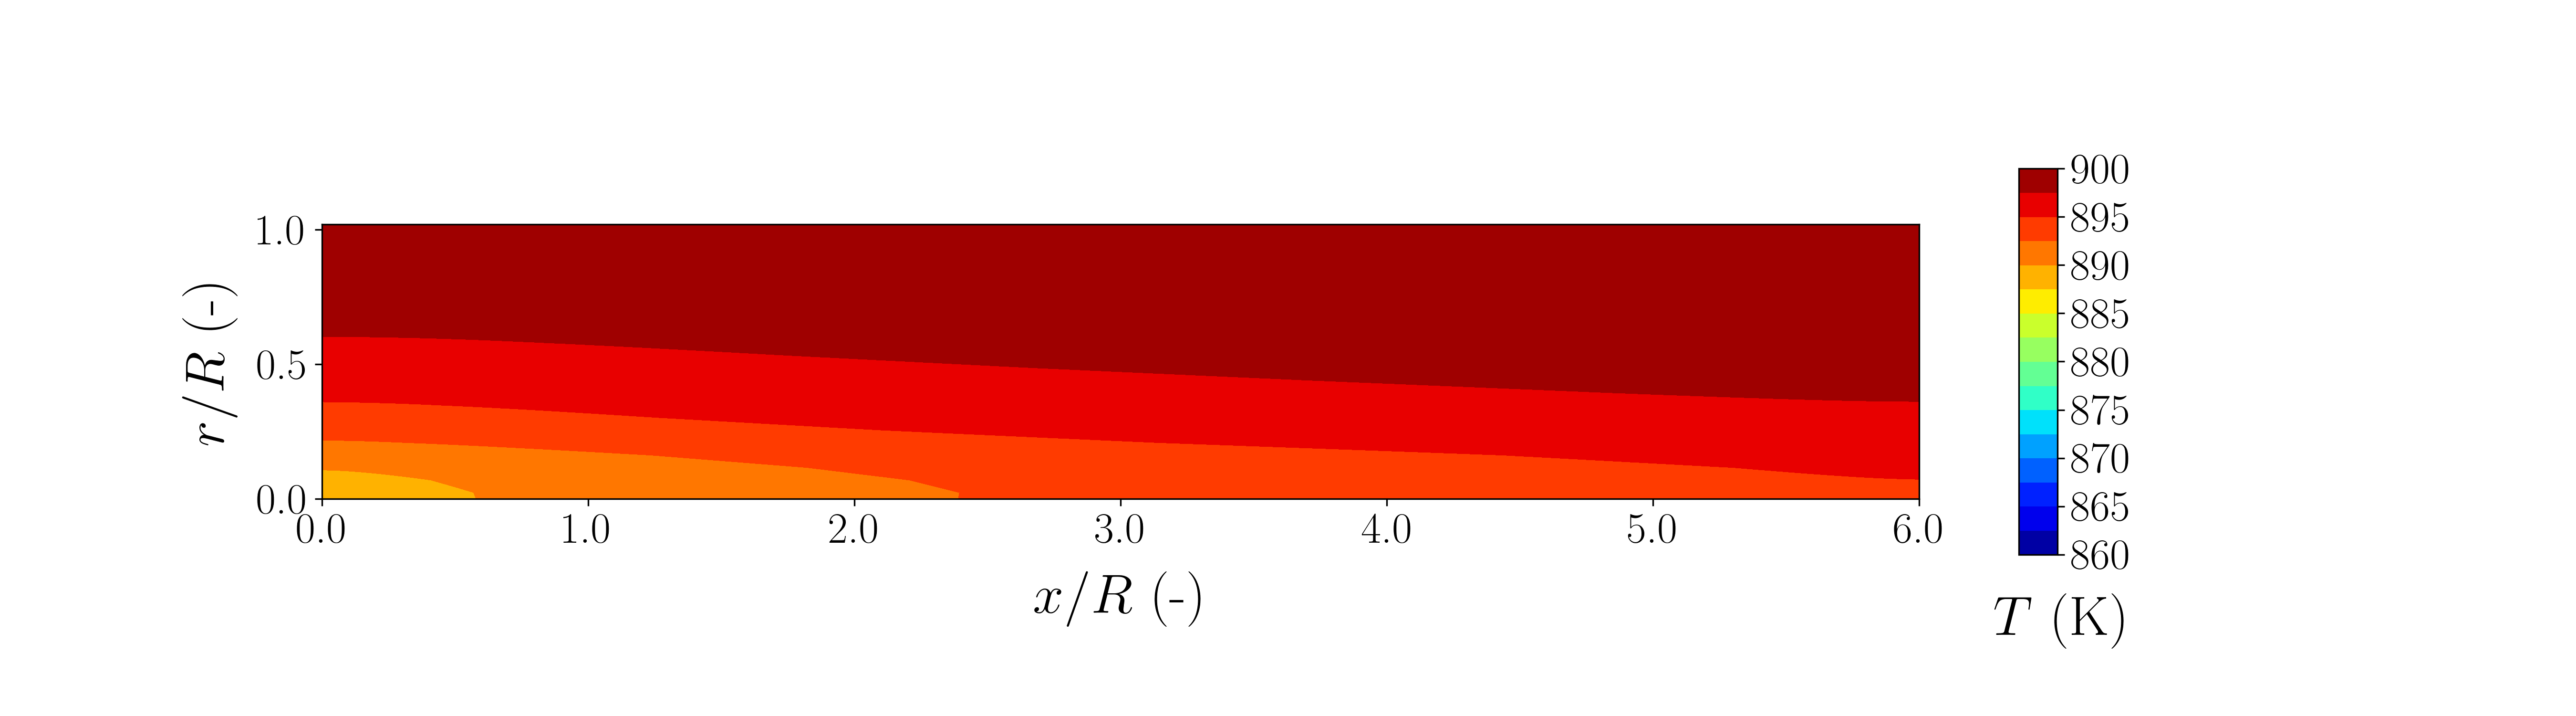
\includegraphics[width=190mm]{results/5/40C_60T/GEN30-TFIELD.png}
%\caption{\label{fig:5R4060G30-TField} Strategy I - Temperature field distribution - 30$^{\rm{th}}$ generation ($w_{\rm{CH_4}} = 0.4, w_T = 0.6$, $T_{\rm{in}}$ = 900 K, $u_{\rm{in}}$ = 0.15 m s$^{-1}$, $SC$ = 2.0)}
%\end{figure}
%
%
%\begin{figure}[h!]
%\centering
%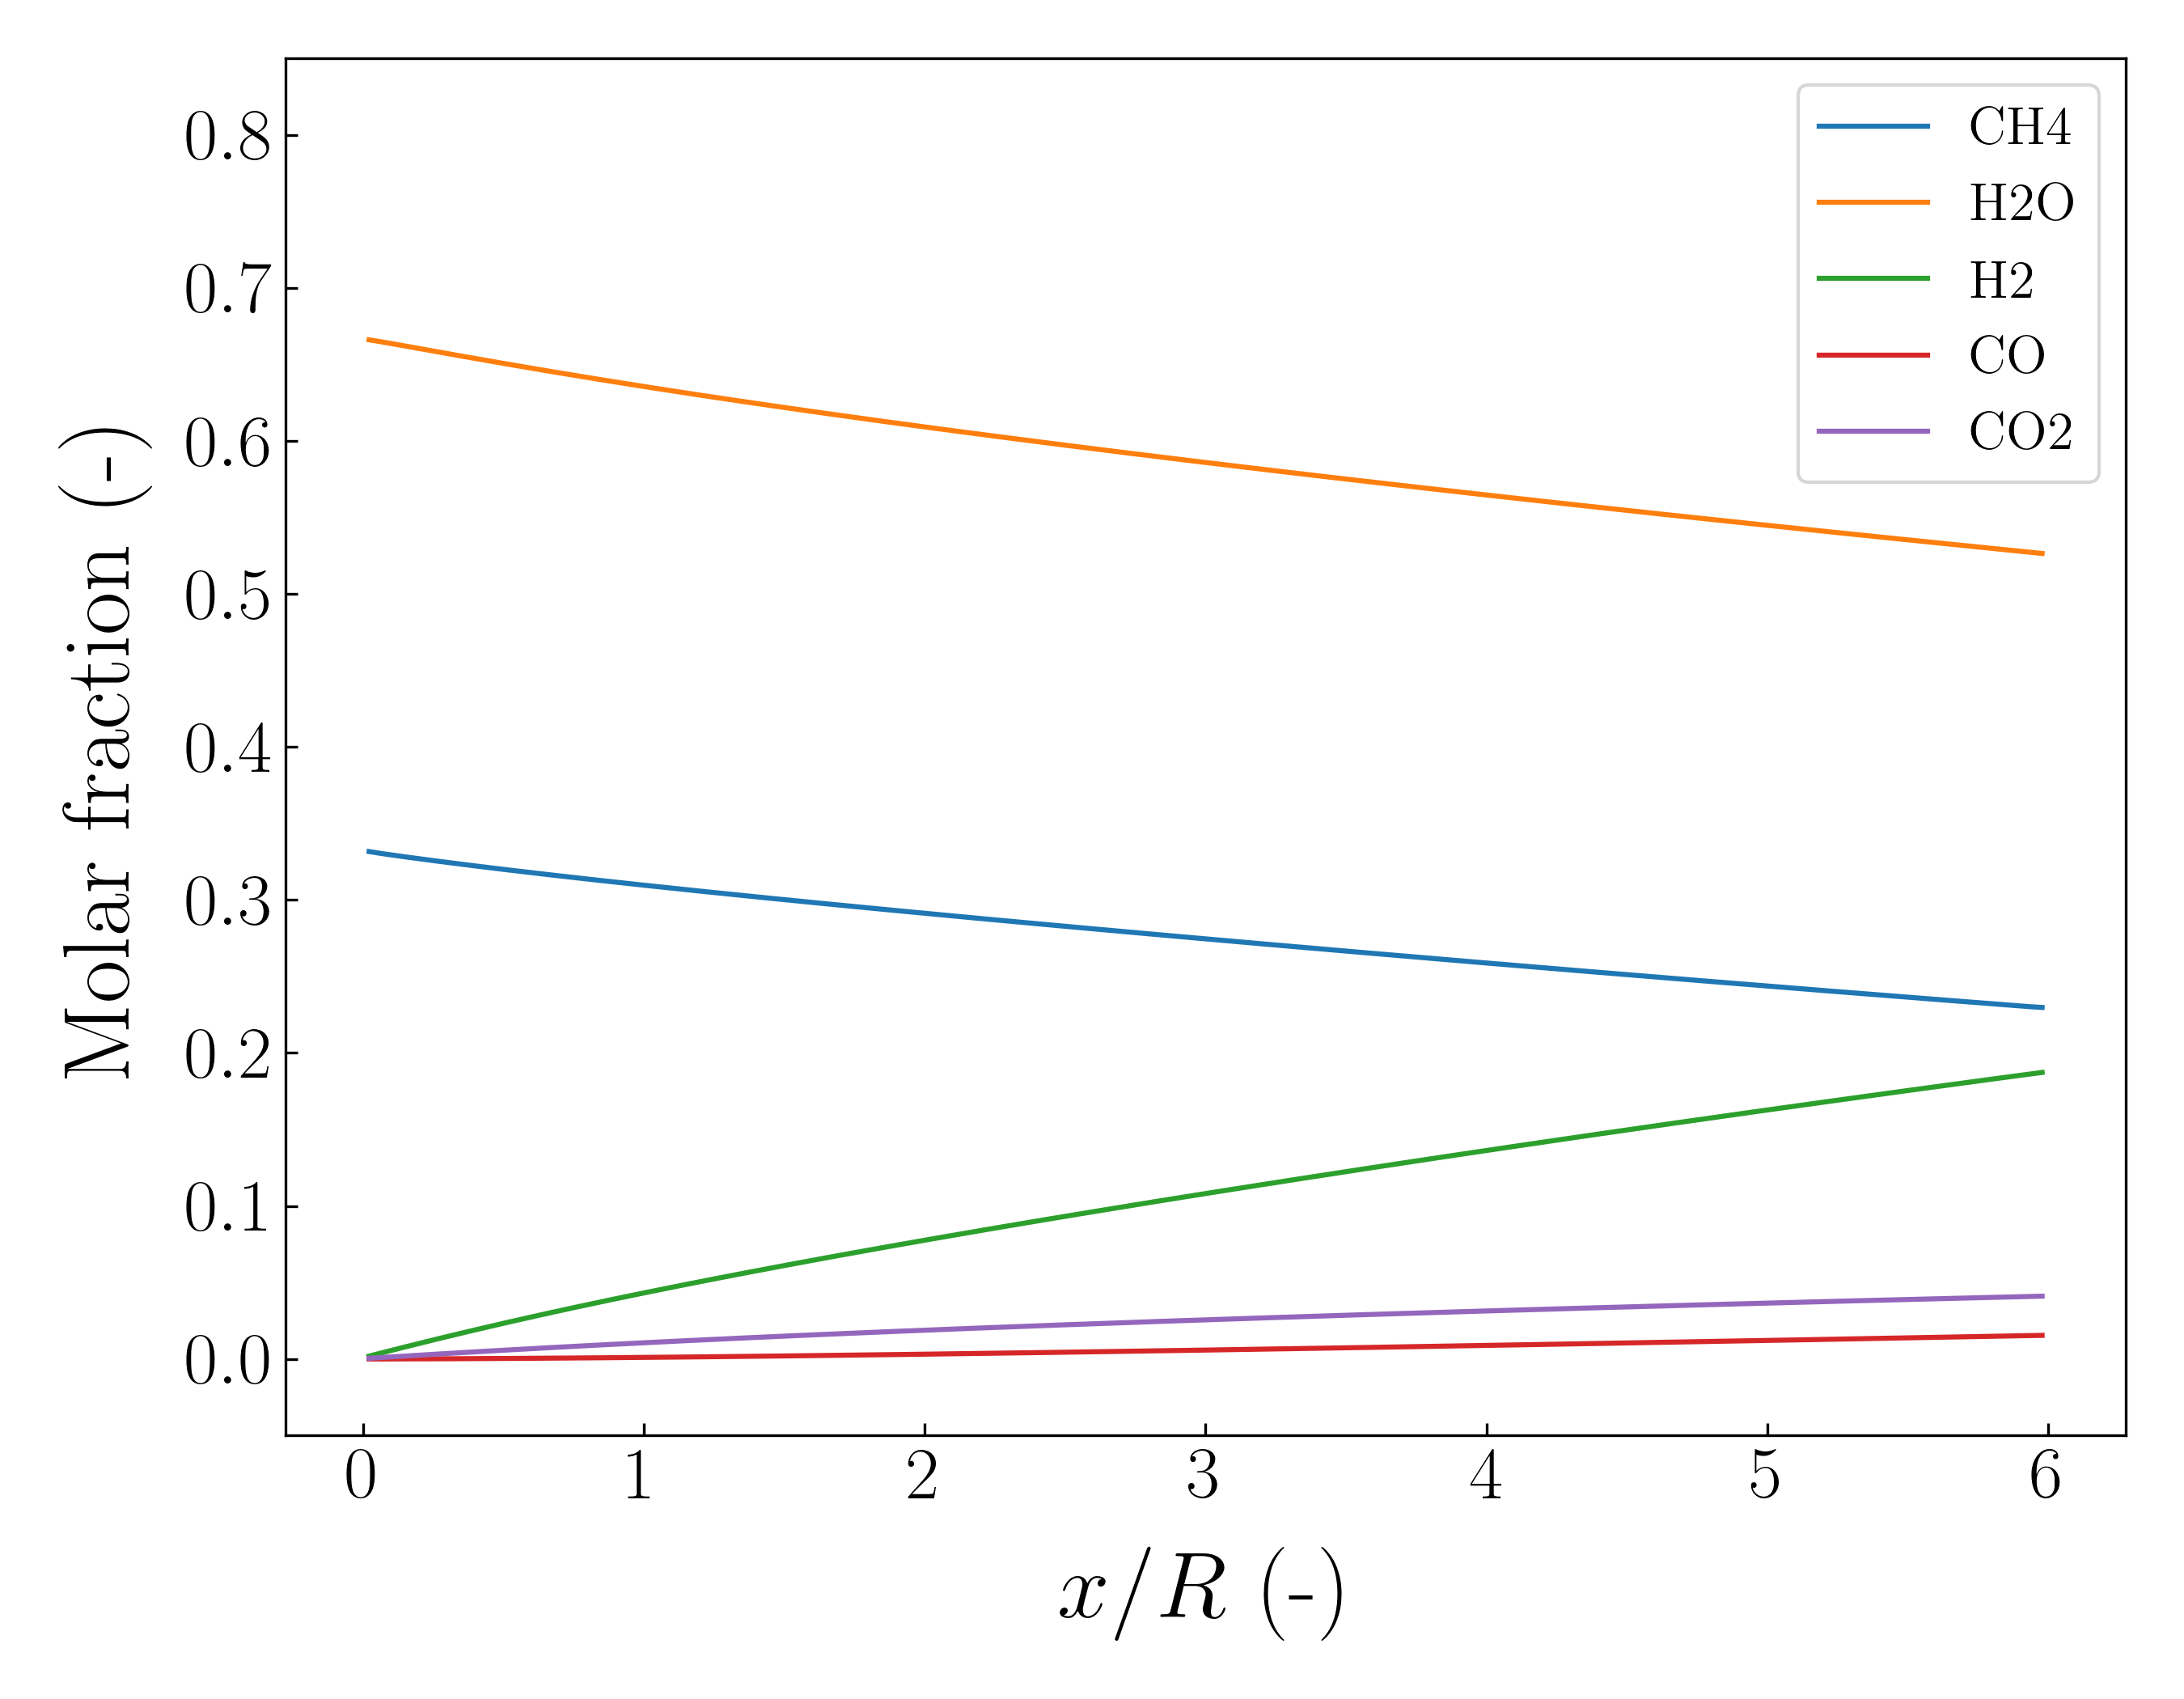
\includegraphics[width=80mm]{results/5/40C_60T/GEN1-AVG.png}
%\caption{\label{fig:5R4060G1-avg} Strategy I - Radius-averaged molar fractions - 1$^{\rm{st}}$ generation ($w_{\rm{CH_4}} = 0.4, w_T = 0.6$, $T_{\rm{in}}$ = 900 K, $u_{\rm{in}}$ = 0.15 m s$^{-1}$, $SC$ = 2.0)}
%\end{figure}
%
%\begin{figure}[h!]
%\centering
%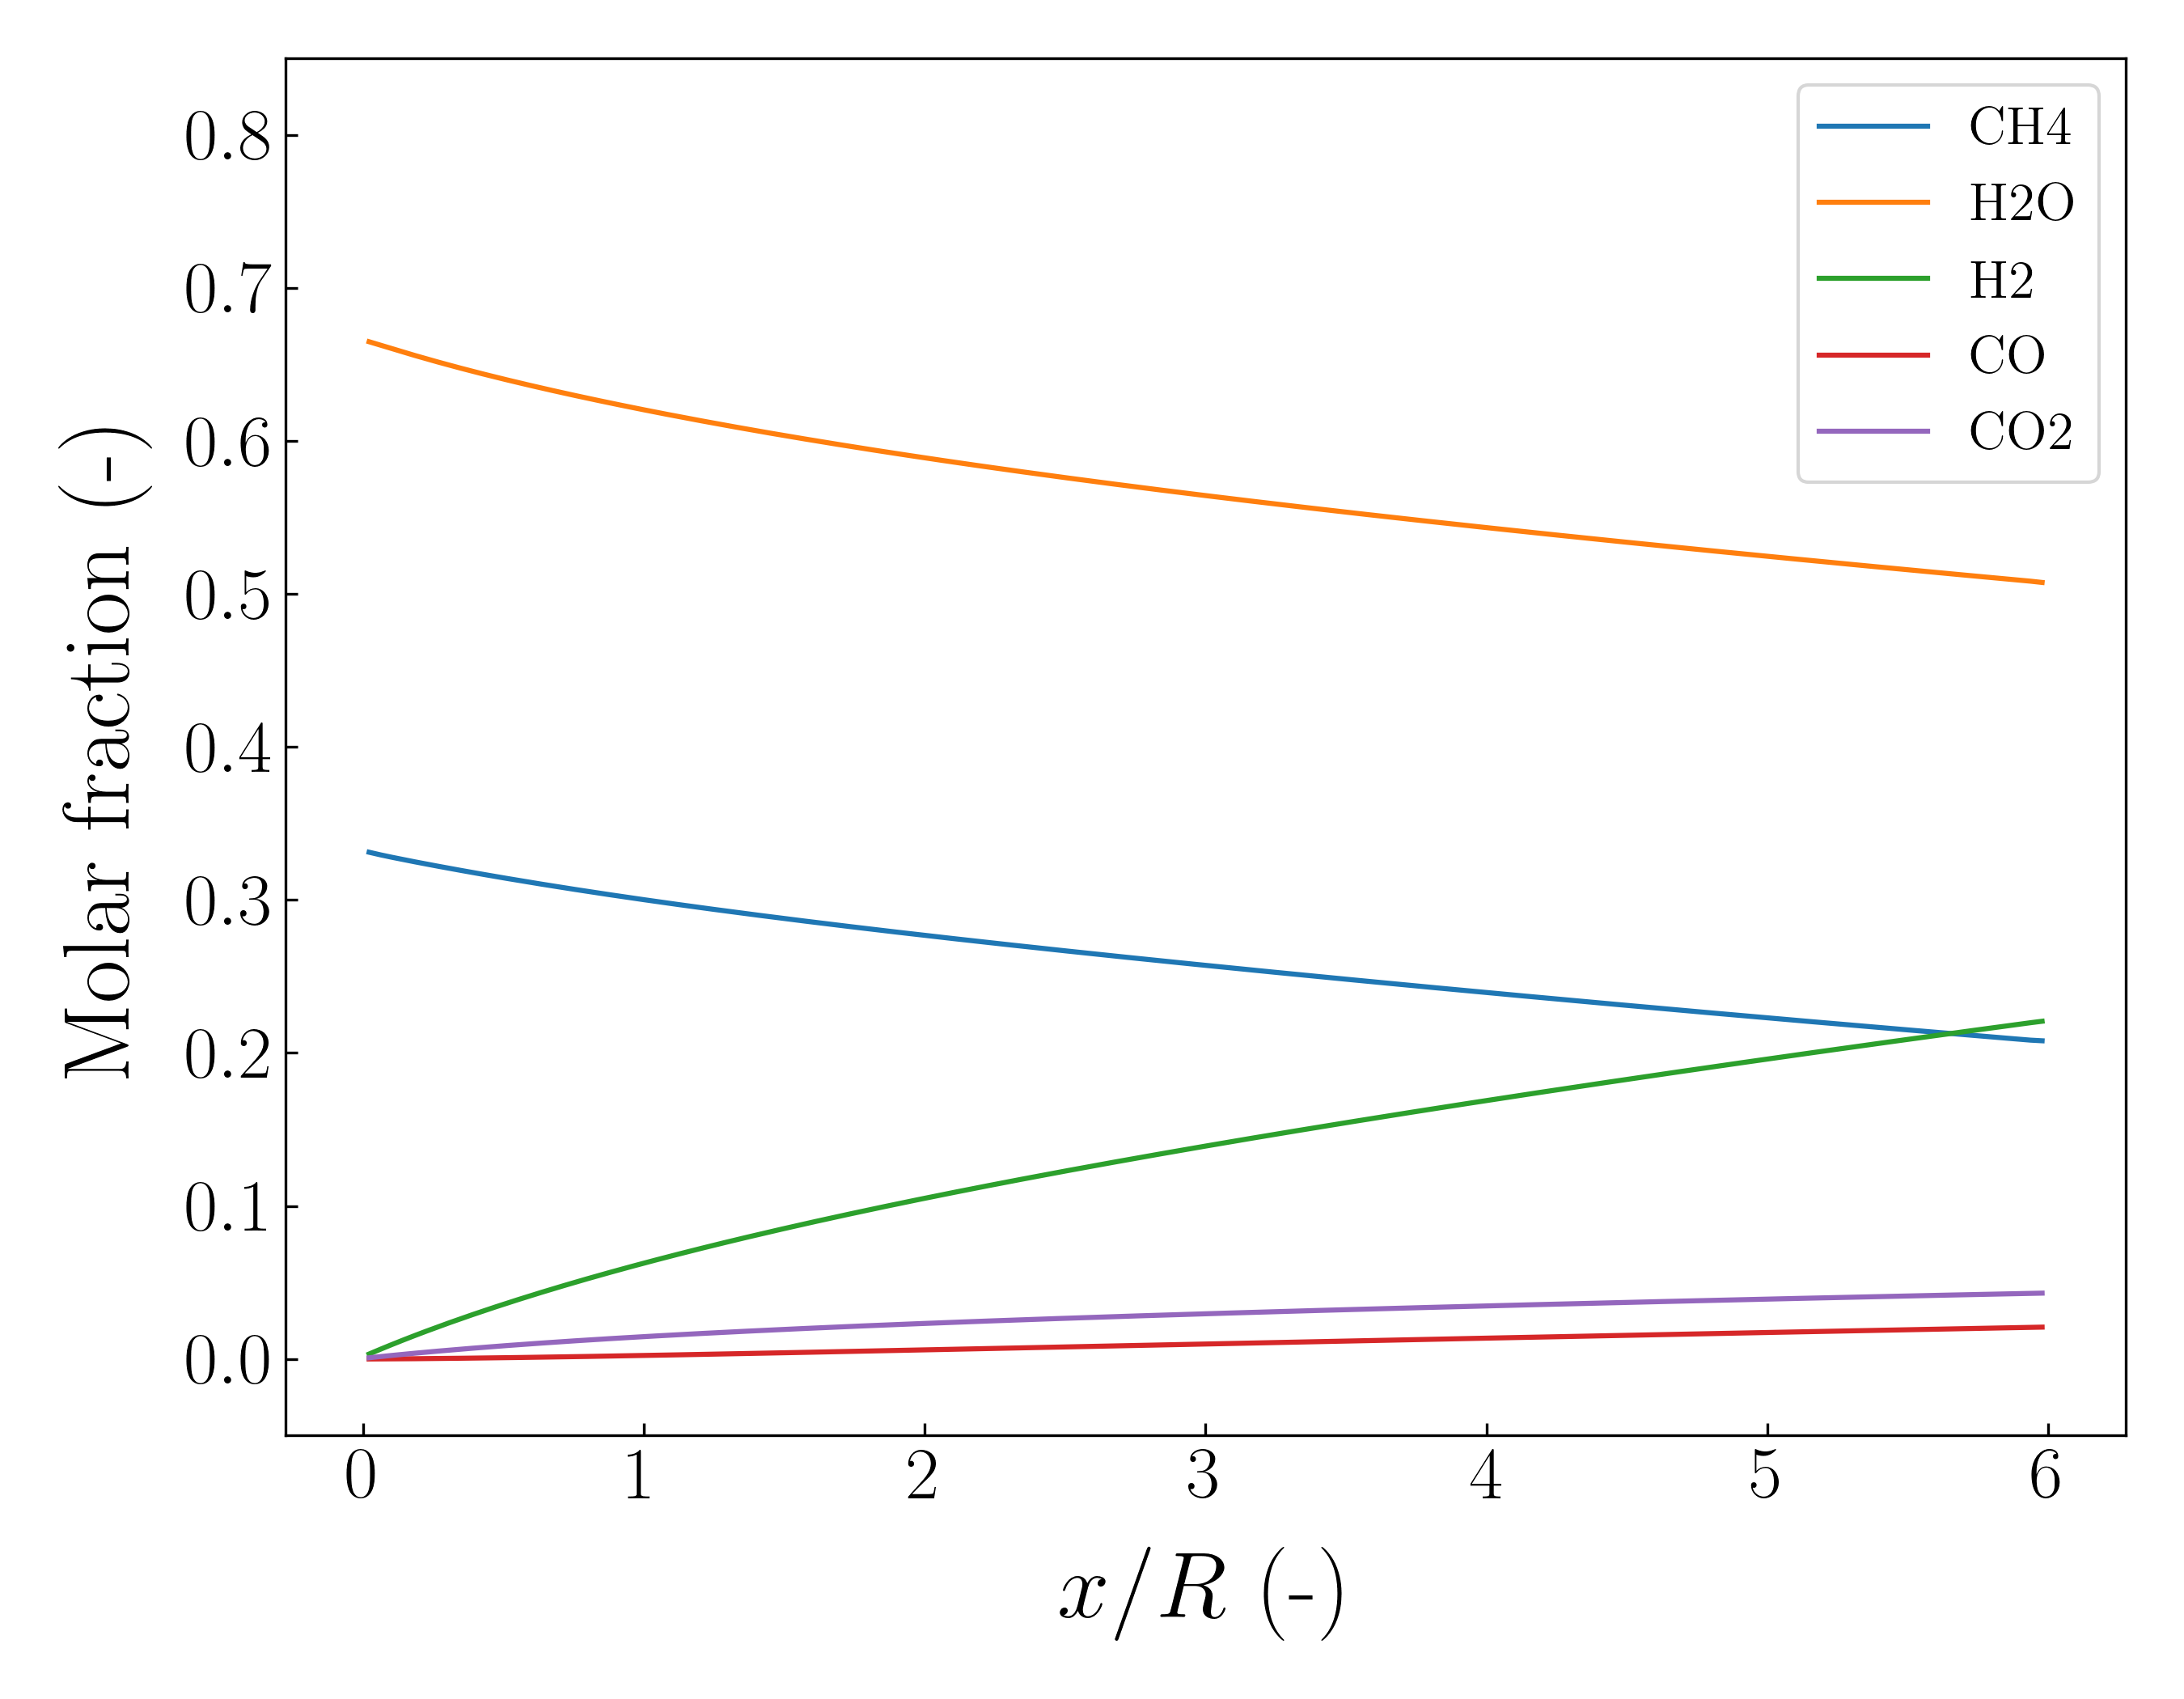
\includegraphics[width=80mm]{results/5/40C_60T/GEN15-AVG.png}
%\caption{\label{fig:5R4060G15-avg} Strategy I - Radius-averaged molar fractions - 15$^{\rm{th}}$ generation ($w_{\rm{CH_4}} = 0.4, w_T = 0.6$, $T_{\rm{in}}$ = 900 K, $u_{\rm{in}}$ = 0.15 m s$^{-1}$, $SC$ = 2.0)}
%\end{figure}
%
%\begin{figure}[h!]
%\centering
%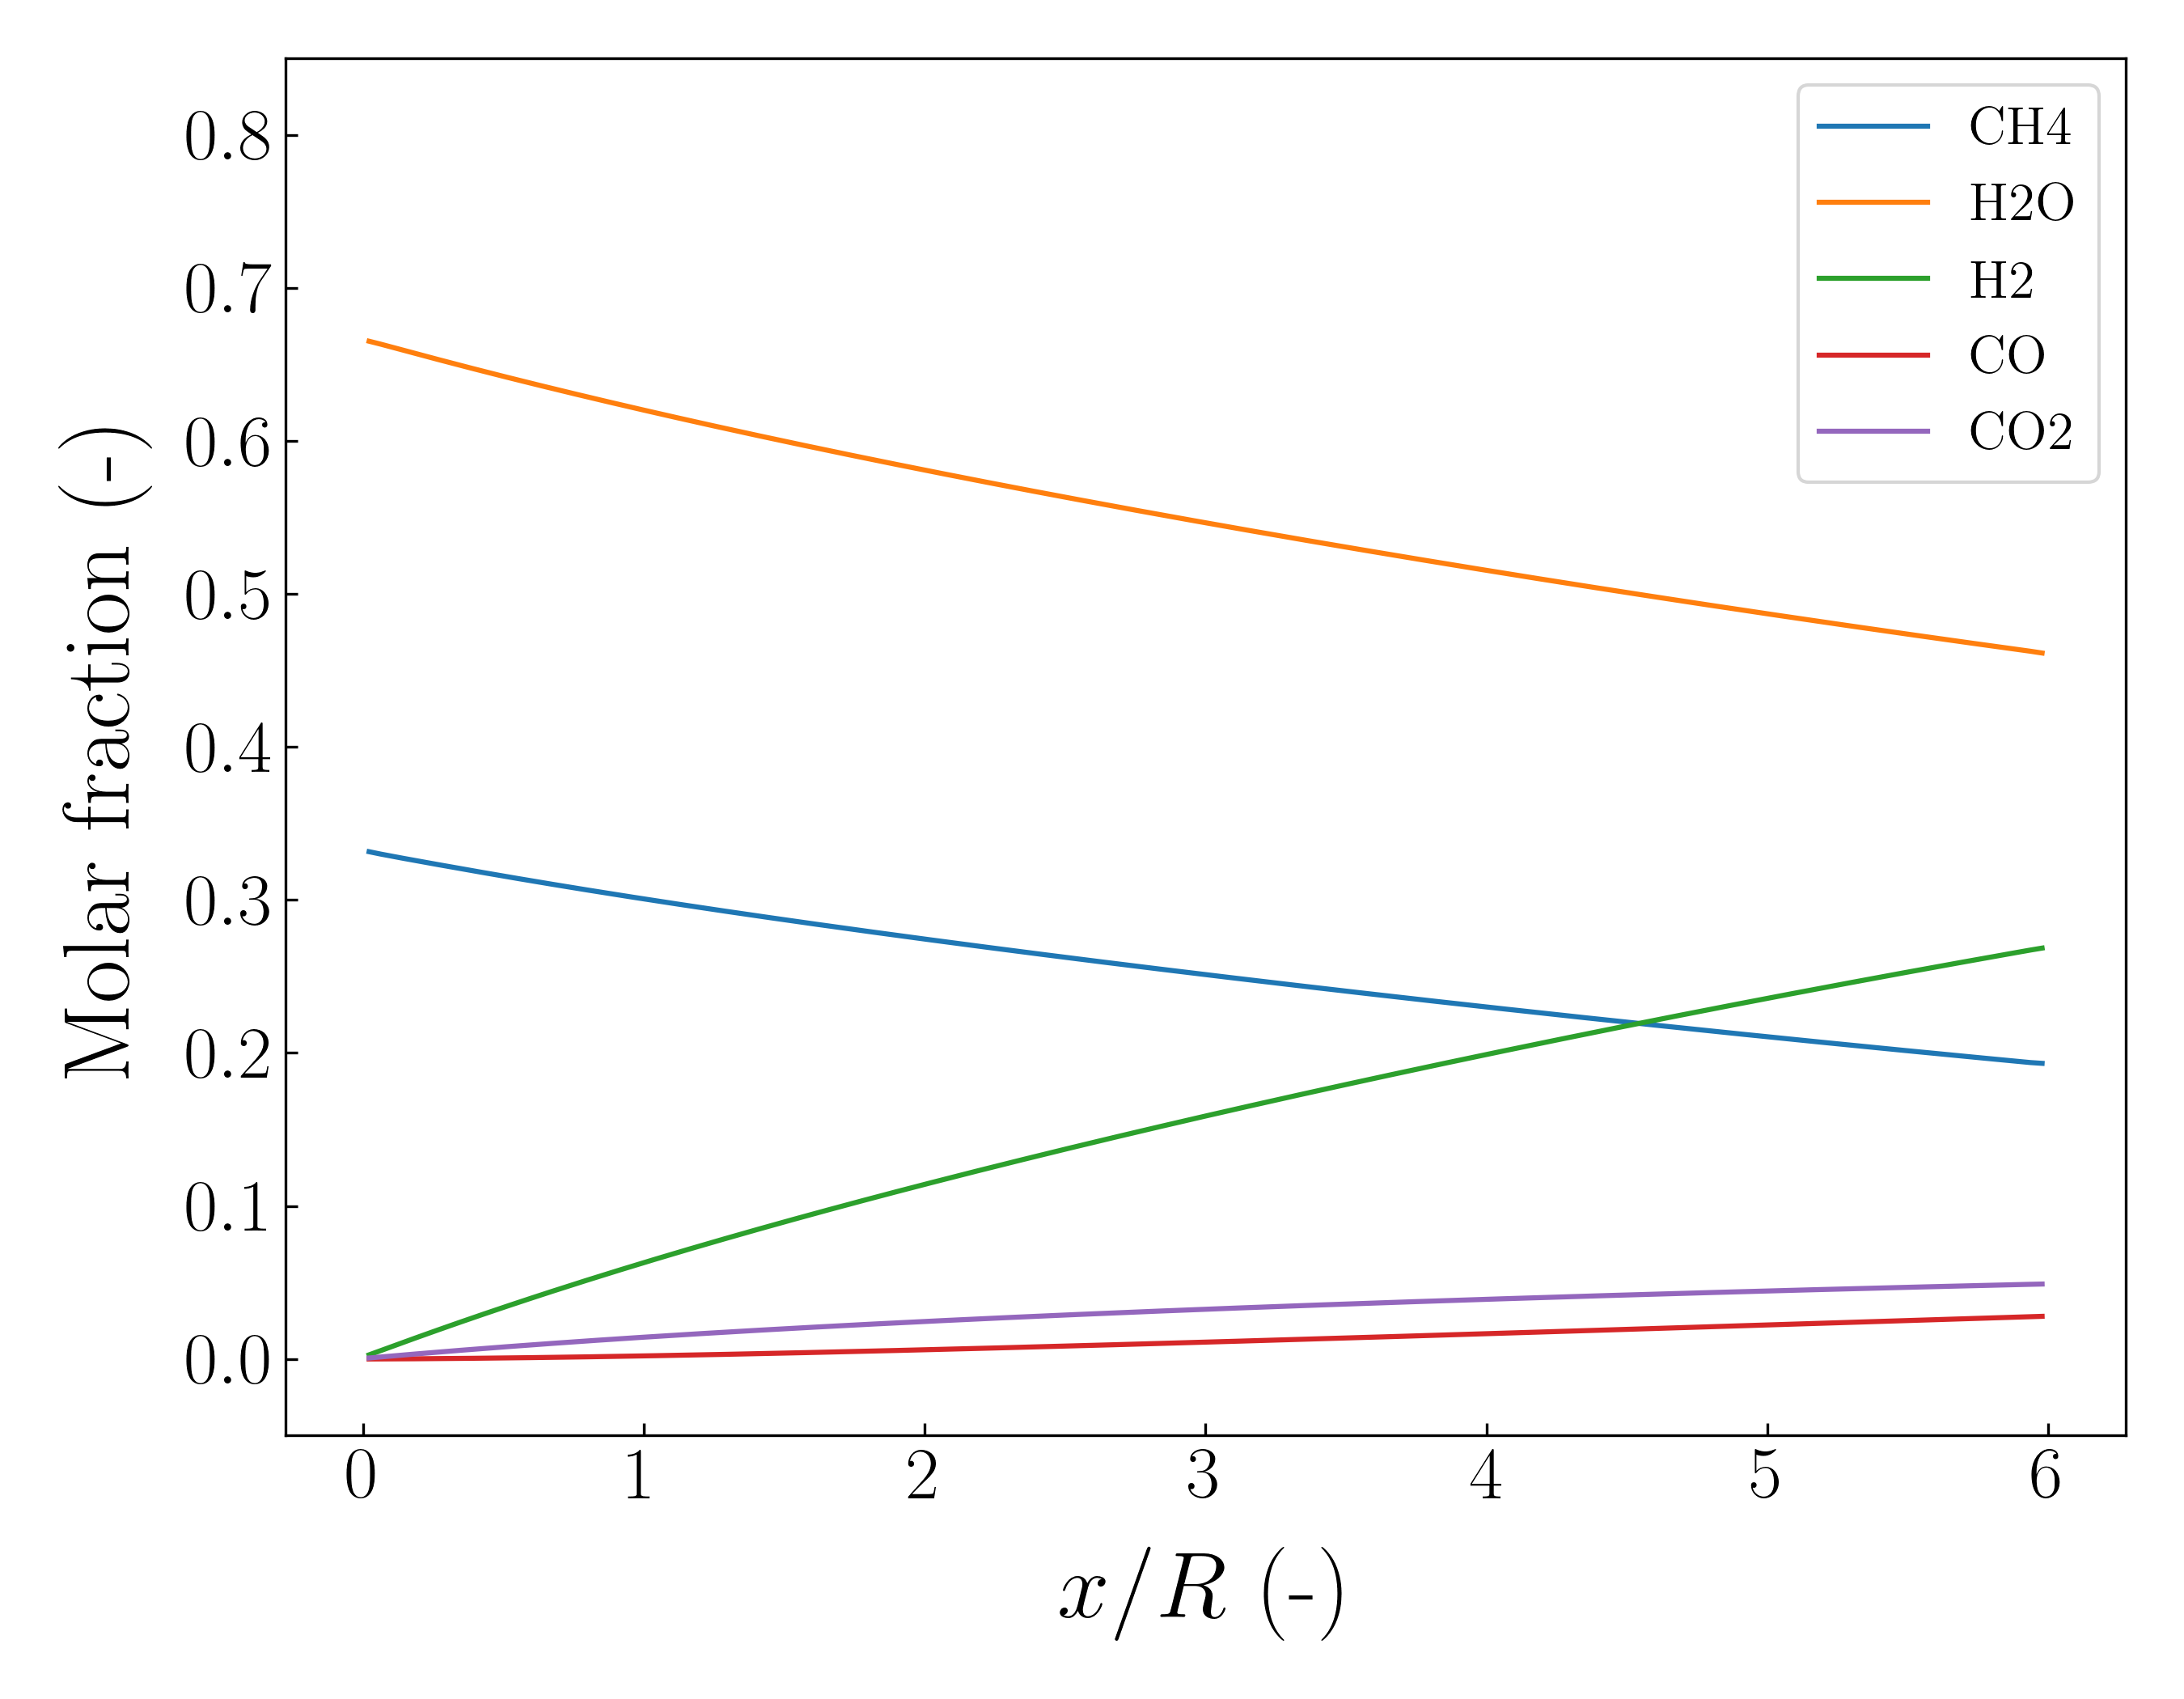
\includegraphics[width=80mm]{results/5/40C_60T/GEN30-AVG.png}
%\caption{\label{fig:5R4060G30-avg} Strategy I - Radius-averaged molar fractions -  30$^{\rm{th}}$ generation ($w_{\rm{CH_4}} = 0.4, w_T = 0.6$, $T_{\rm{in}}$ = 900 K, $u_{\rm{in}}$ = 0.15 m s$^{-1}$, $SC$ = 2.0)}
%\end{figure}
%
%\begin{figure}[h!]
%\centering
%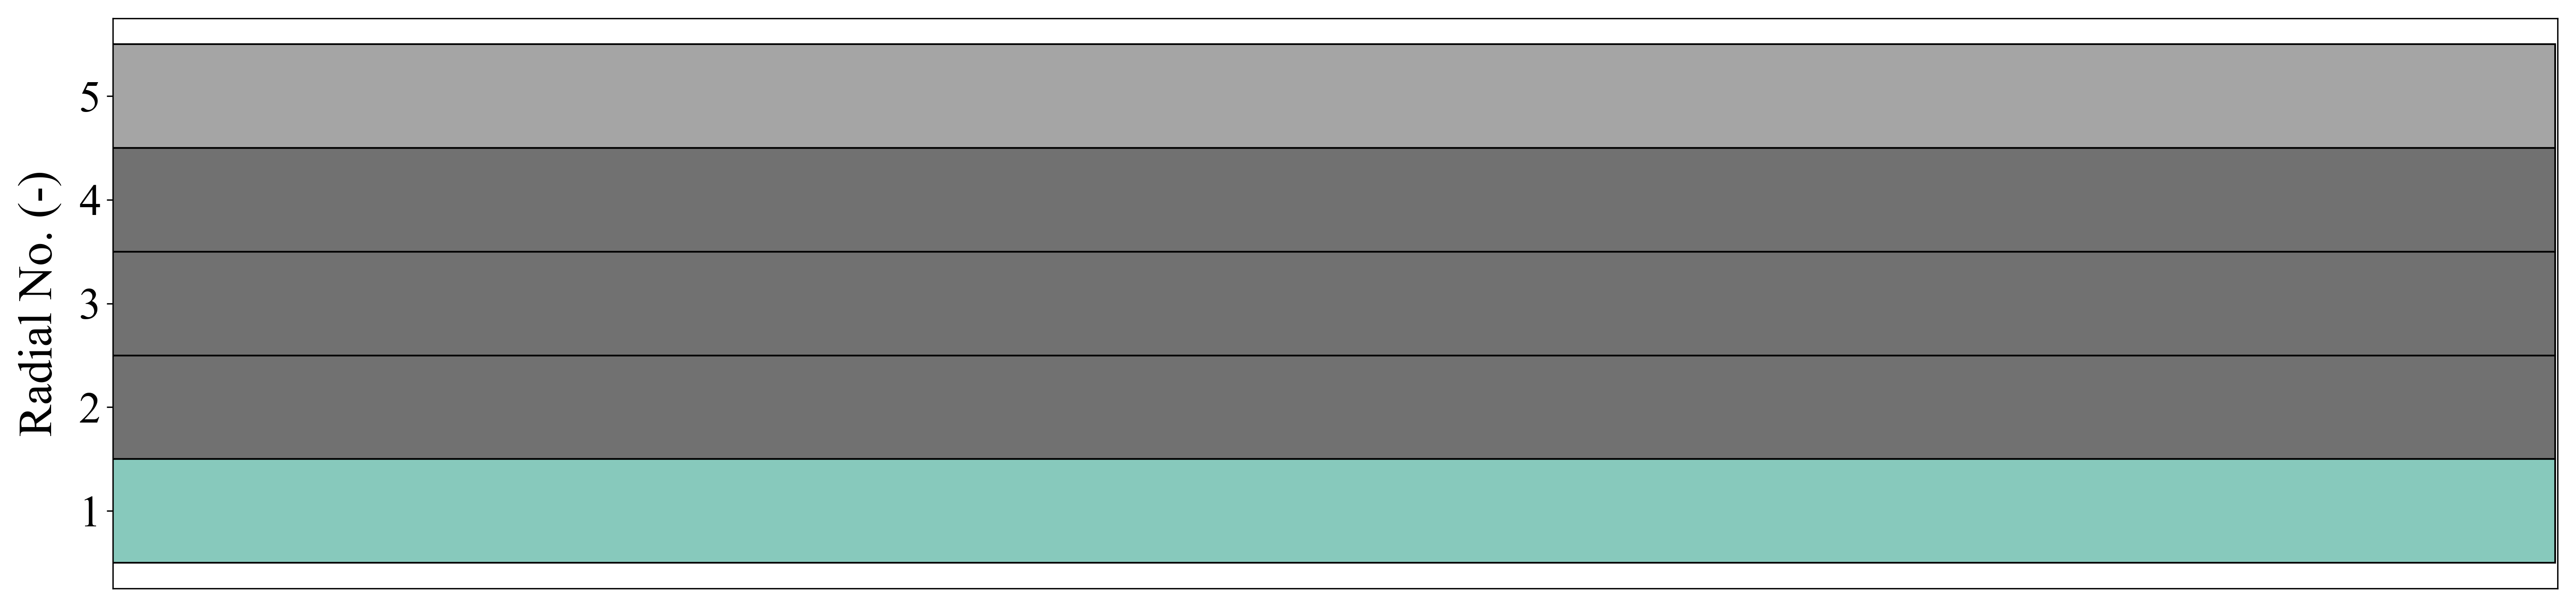
\includegraphics[width=120mm]{results/segments/5seg/40C60T/seg.png}
%\caption{\label{fig:30L6040G1-TField} Strategy I - Segments distribution for 30$^{\rm{th}}$ generation ($w_{\rm{CH_4}} = 0.4, w_T = 0.6$, $T_{\rm{in}}$ = 900 K, $u_{\rm{in}}$ = 0.15 m s$^{-1}$, $SC$ = 2.0)}
%\end{figure}
%
%\begin{figure}[h!]
%\centering
%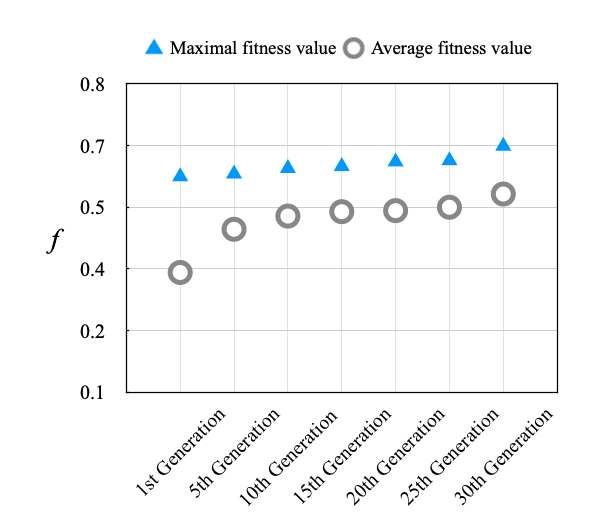
\includegraphics[width=100mm]{results/5/40C_60T.png}
%\caption{\label{fig:5R4060G-fitness} Strategy I - Fitness analysis throughout successive populations ($w_{\rm{CH_4}} = 0.4, w_T = 0.6$, $T_{\rm{in}}$ = 900 K, $u_{\rm{in}}$ = 0.15 m s$^{-1}$, $SC$ = 2.0)}
%\end{figure}
%
%
%\clearpage
%
%
%
%
%
%\paragraph{Thermal fitness 50 \%, methane conversion 50 \%} \hspace{0pt} \\
%\noindent 
%
%
%\begin{figure}[h!]
%\centering
%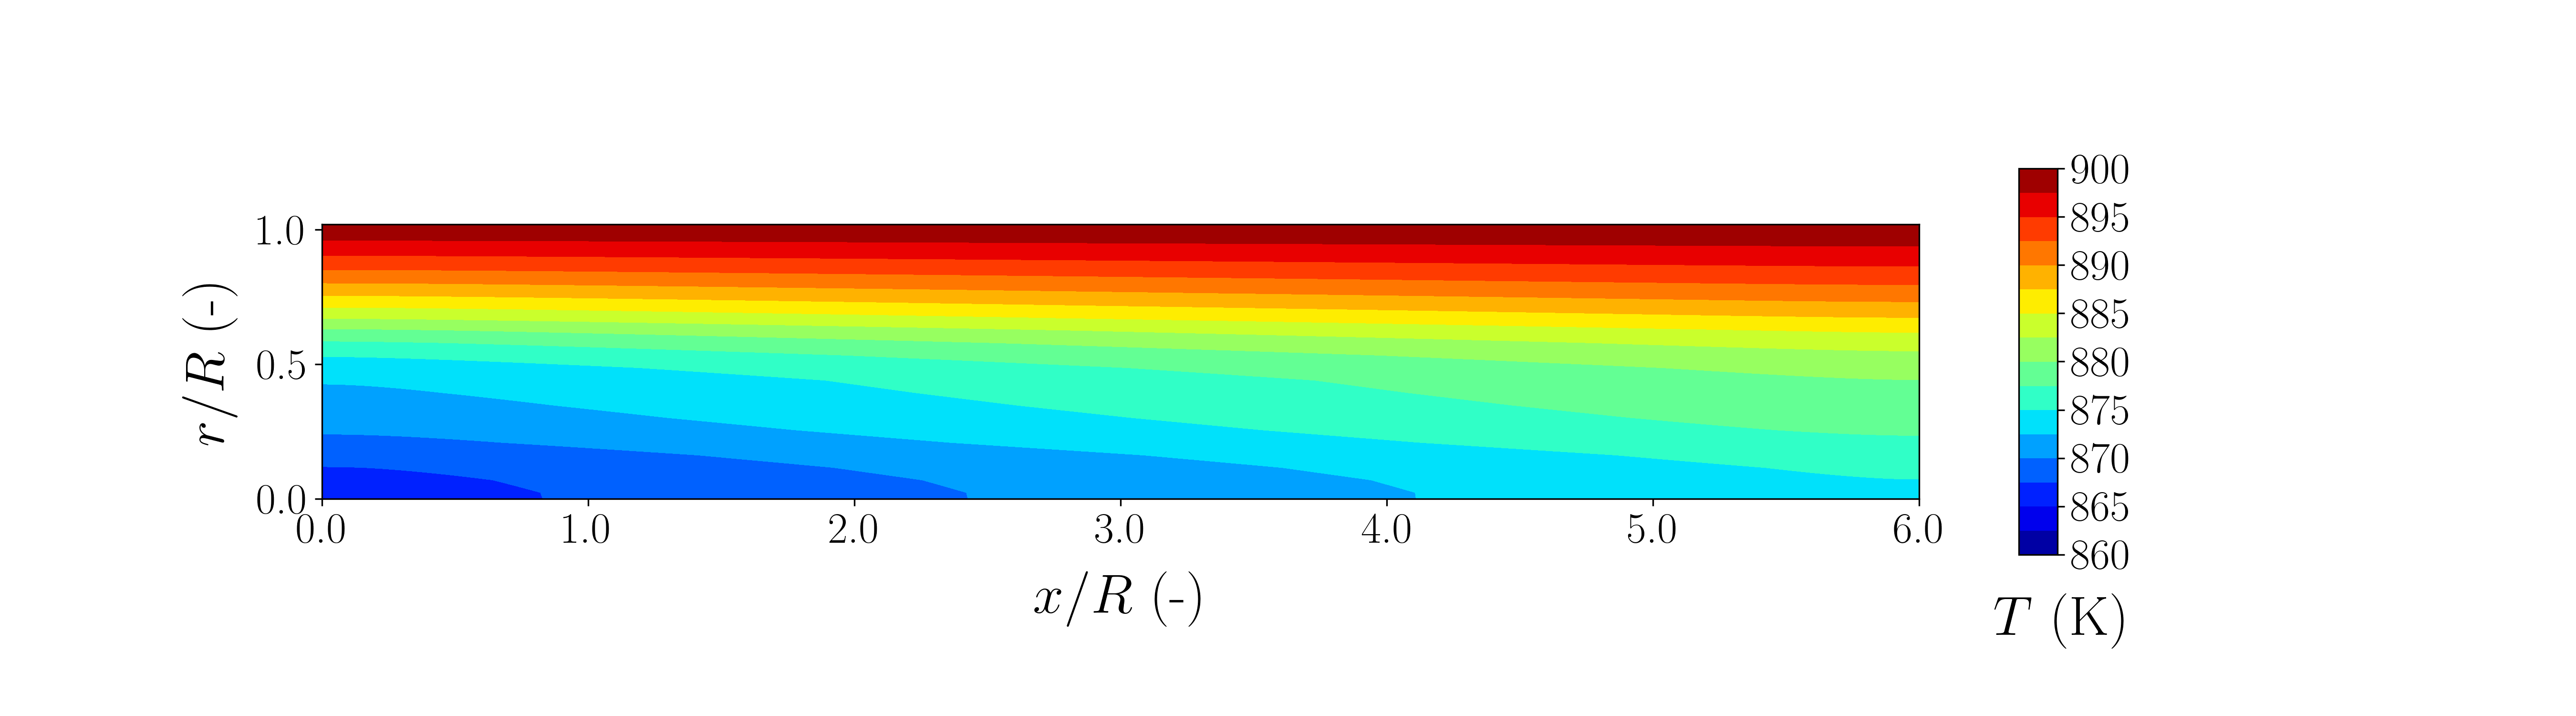
\includegraphics[width=190mm]{results/5/50C_50T/GEN1-TFIELD.png}
%\caption{\label{fig:5R5050G1-TField} Strategy I - Temperature field distribution - 1$^{\rm{st}}$ generation ($w_{\rm{CH_4}} = 0.5, w_T = 0.5$, $T_{\rm{in}}$ = 900 K, $u_{\rm{in}}$ = 0.15 m s$^{-1}$, $SC$ = 2.0)}
%\end{figure}
%
%\begin{figure}[h!]
%\centering
%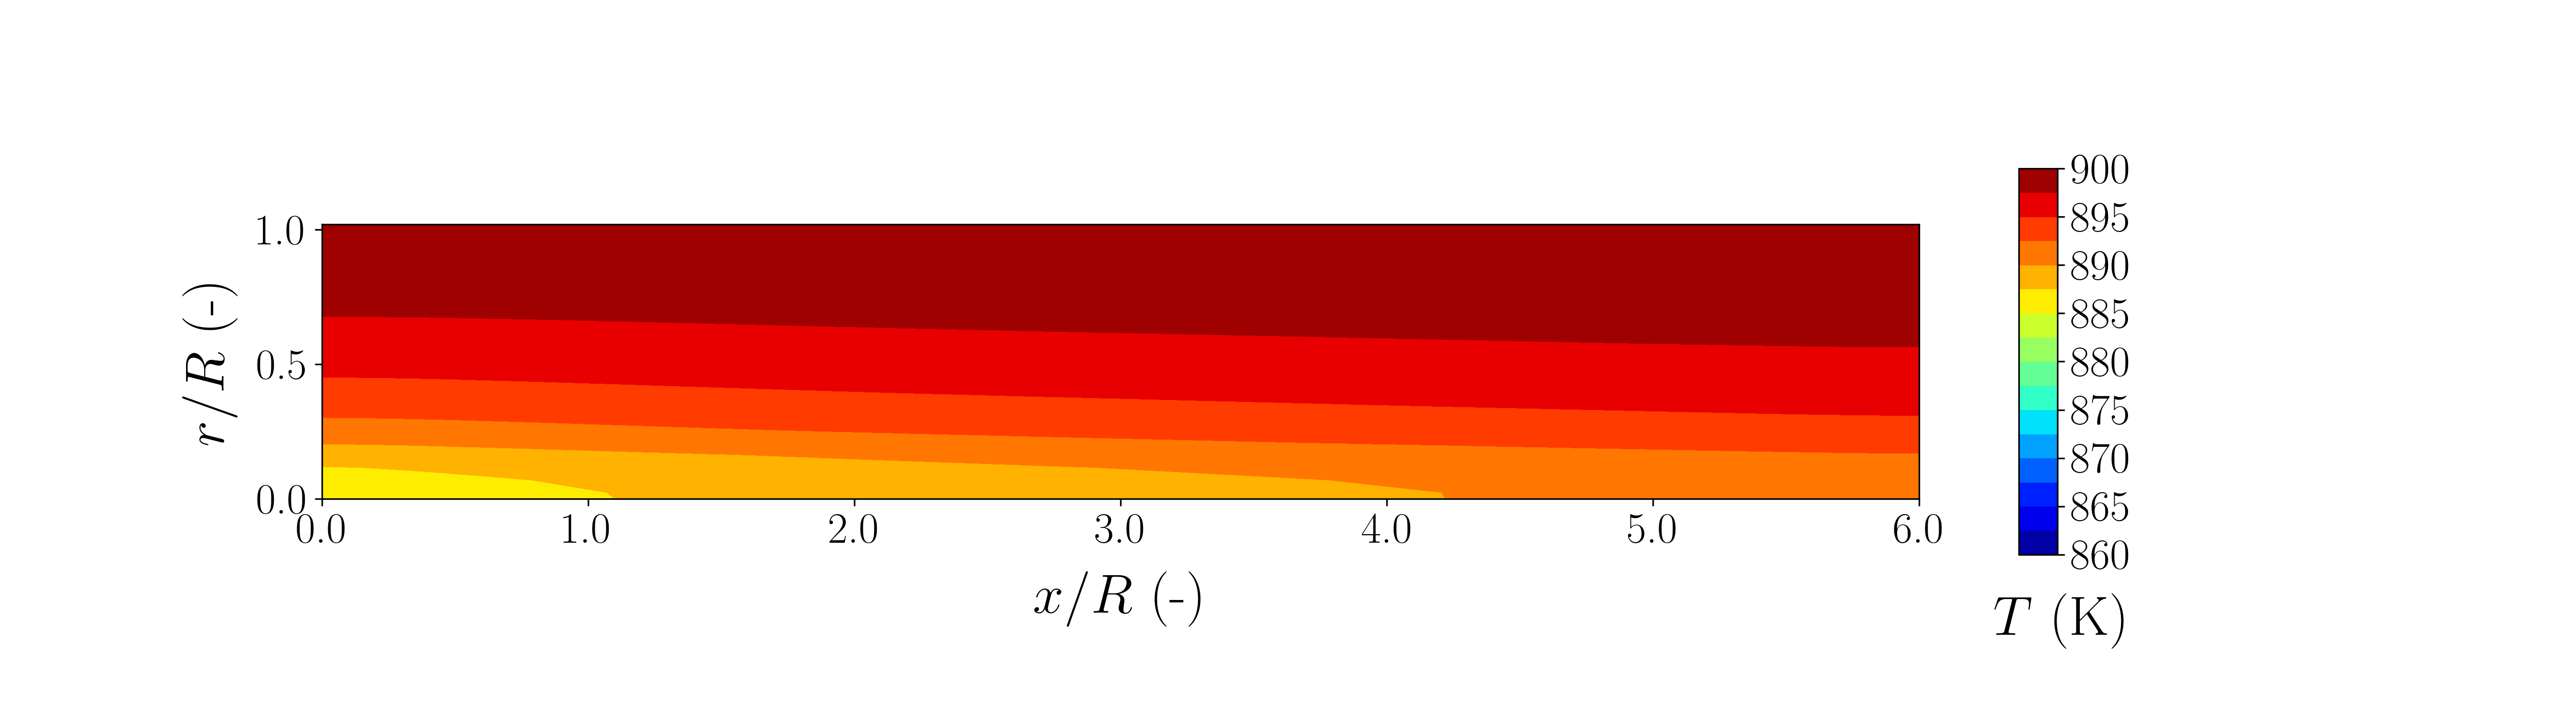
\includegraphics[width=190mm]{results/5/50C_50T/GEN15-TFIELD.png}
%\caption{\label{fig:5R5050G15-TField} Strategy I - Temperature field distribution - 15$^{\rm{th}}$ generation ($w_{\rm{CH_4}} = 0.5, w_T = 0.5$, $T_{\rm{in}}$ = 900 K, $u_{\rm{in}}$ = 0.15 m s$^{-1}$, $SC$ = 2.0)}
%\end{figure}
%
%\begin{figure}[h!]
%\centering
%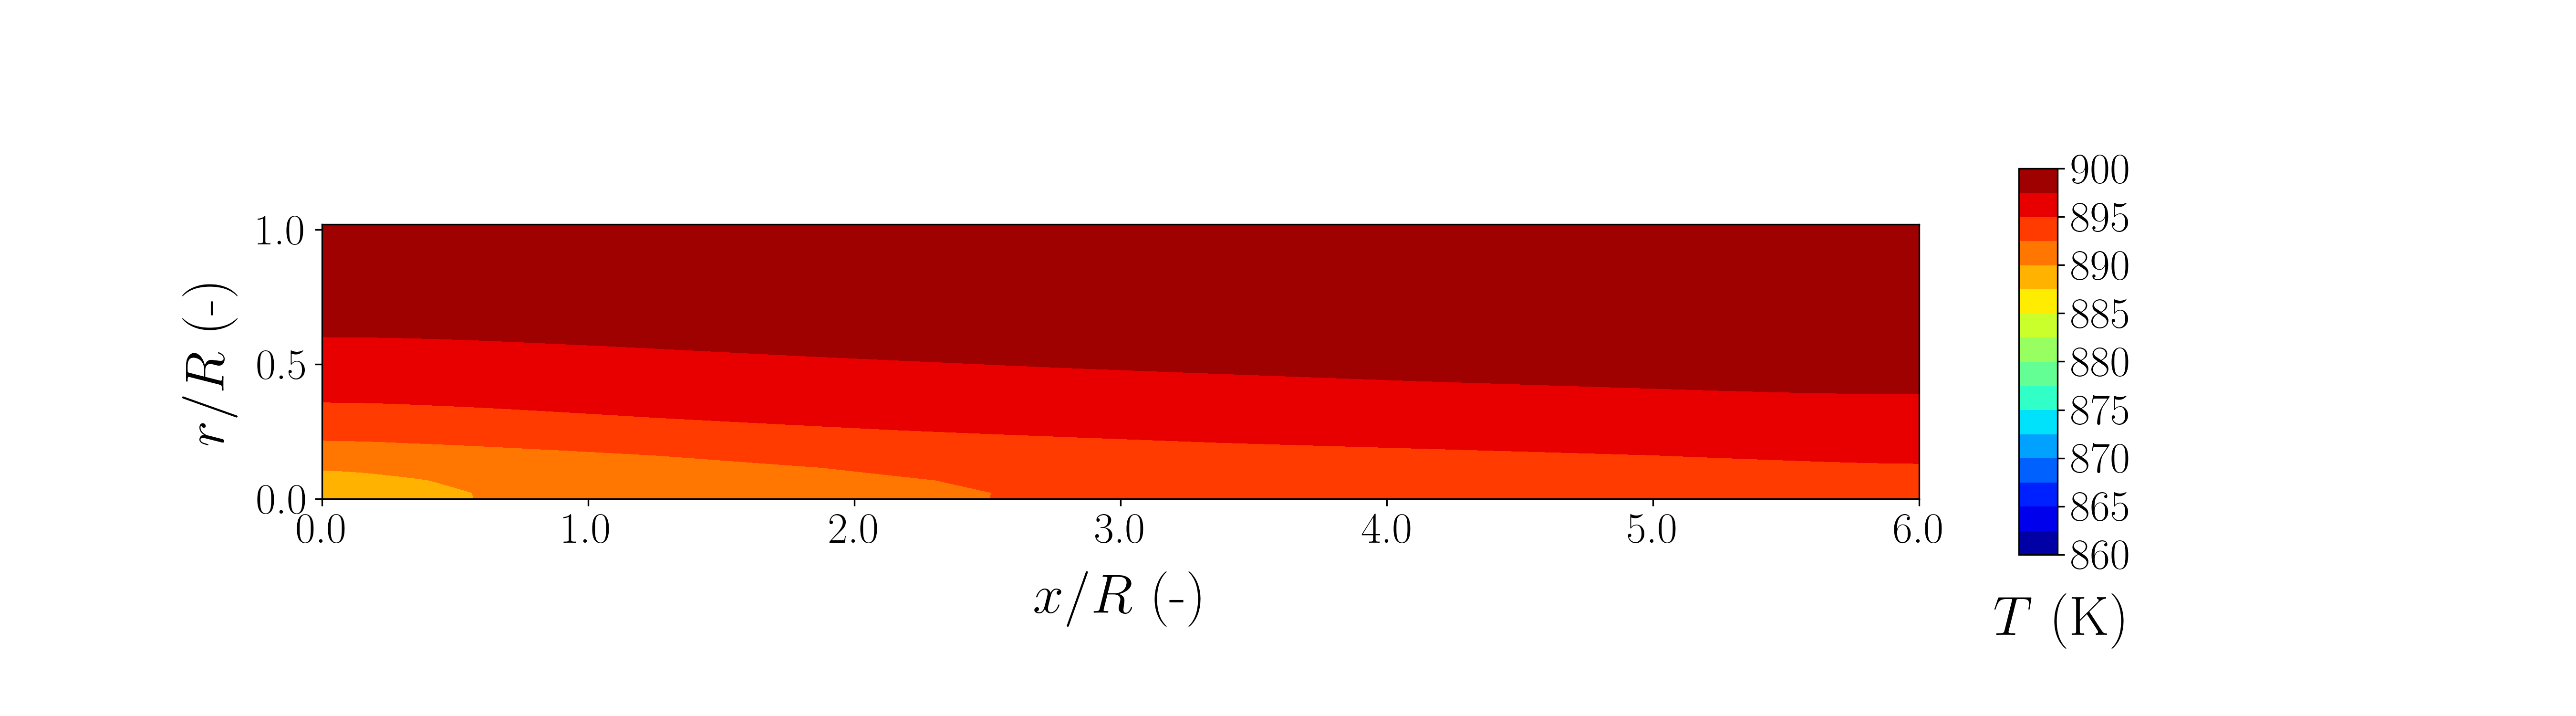
\includegraphics[width=190mm]{results/5/50C_50T/GEN30-TFIELD.png}
%\caption{\label{fig:5R5050G30-TField} Strategy I - Temperature field distribution - 30$^{\rm{th}}$ generation ($w_{\rm{CH_4}} = 0.5, w_T = 0.5$, $T_{\rm{in}}$ = 900 K, $u_{\rm{in}}$ = 0.15 m s$^{-1}$, $SC$ = 2.0)}
%\end{figure}
%
%
%\begin{figure}[h!]
%\centering
%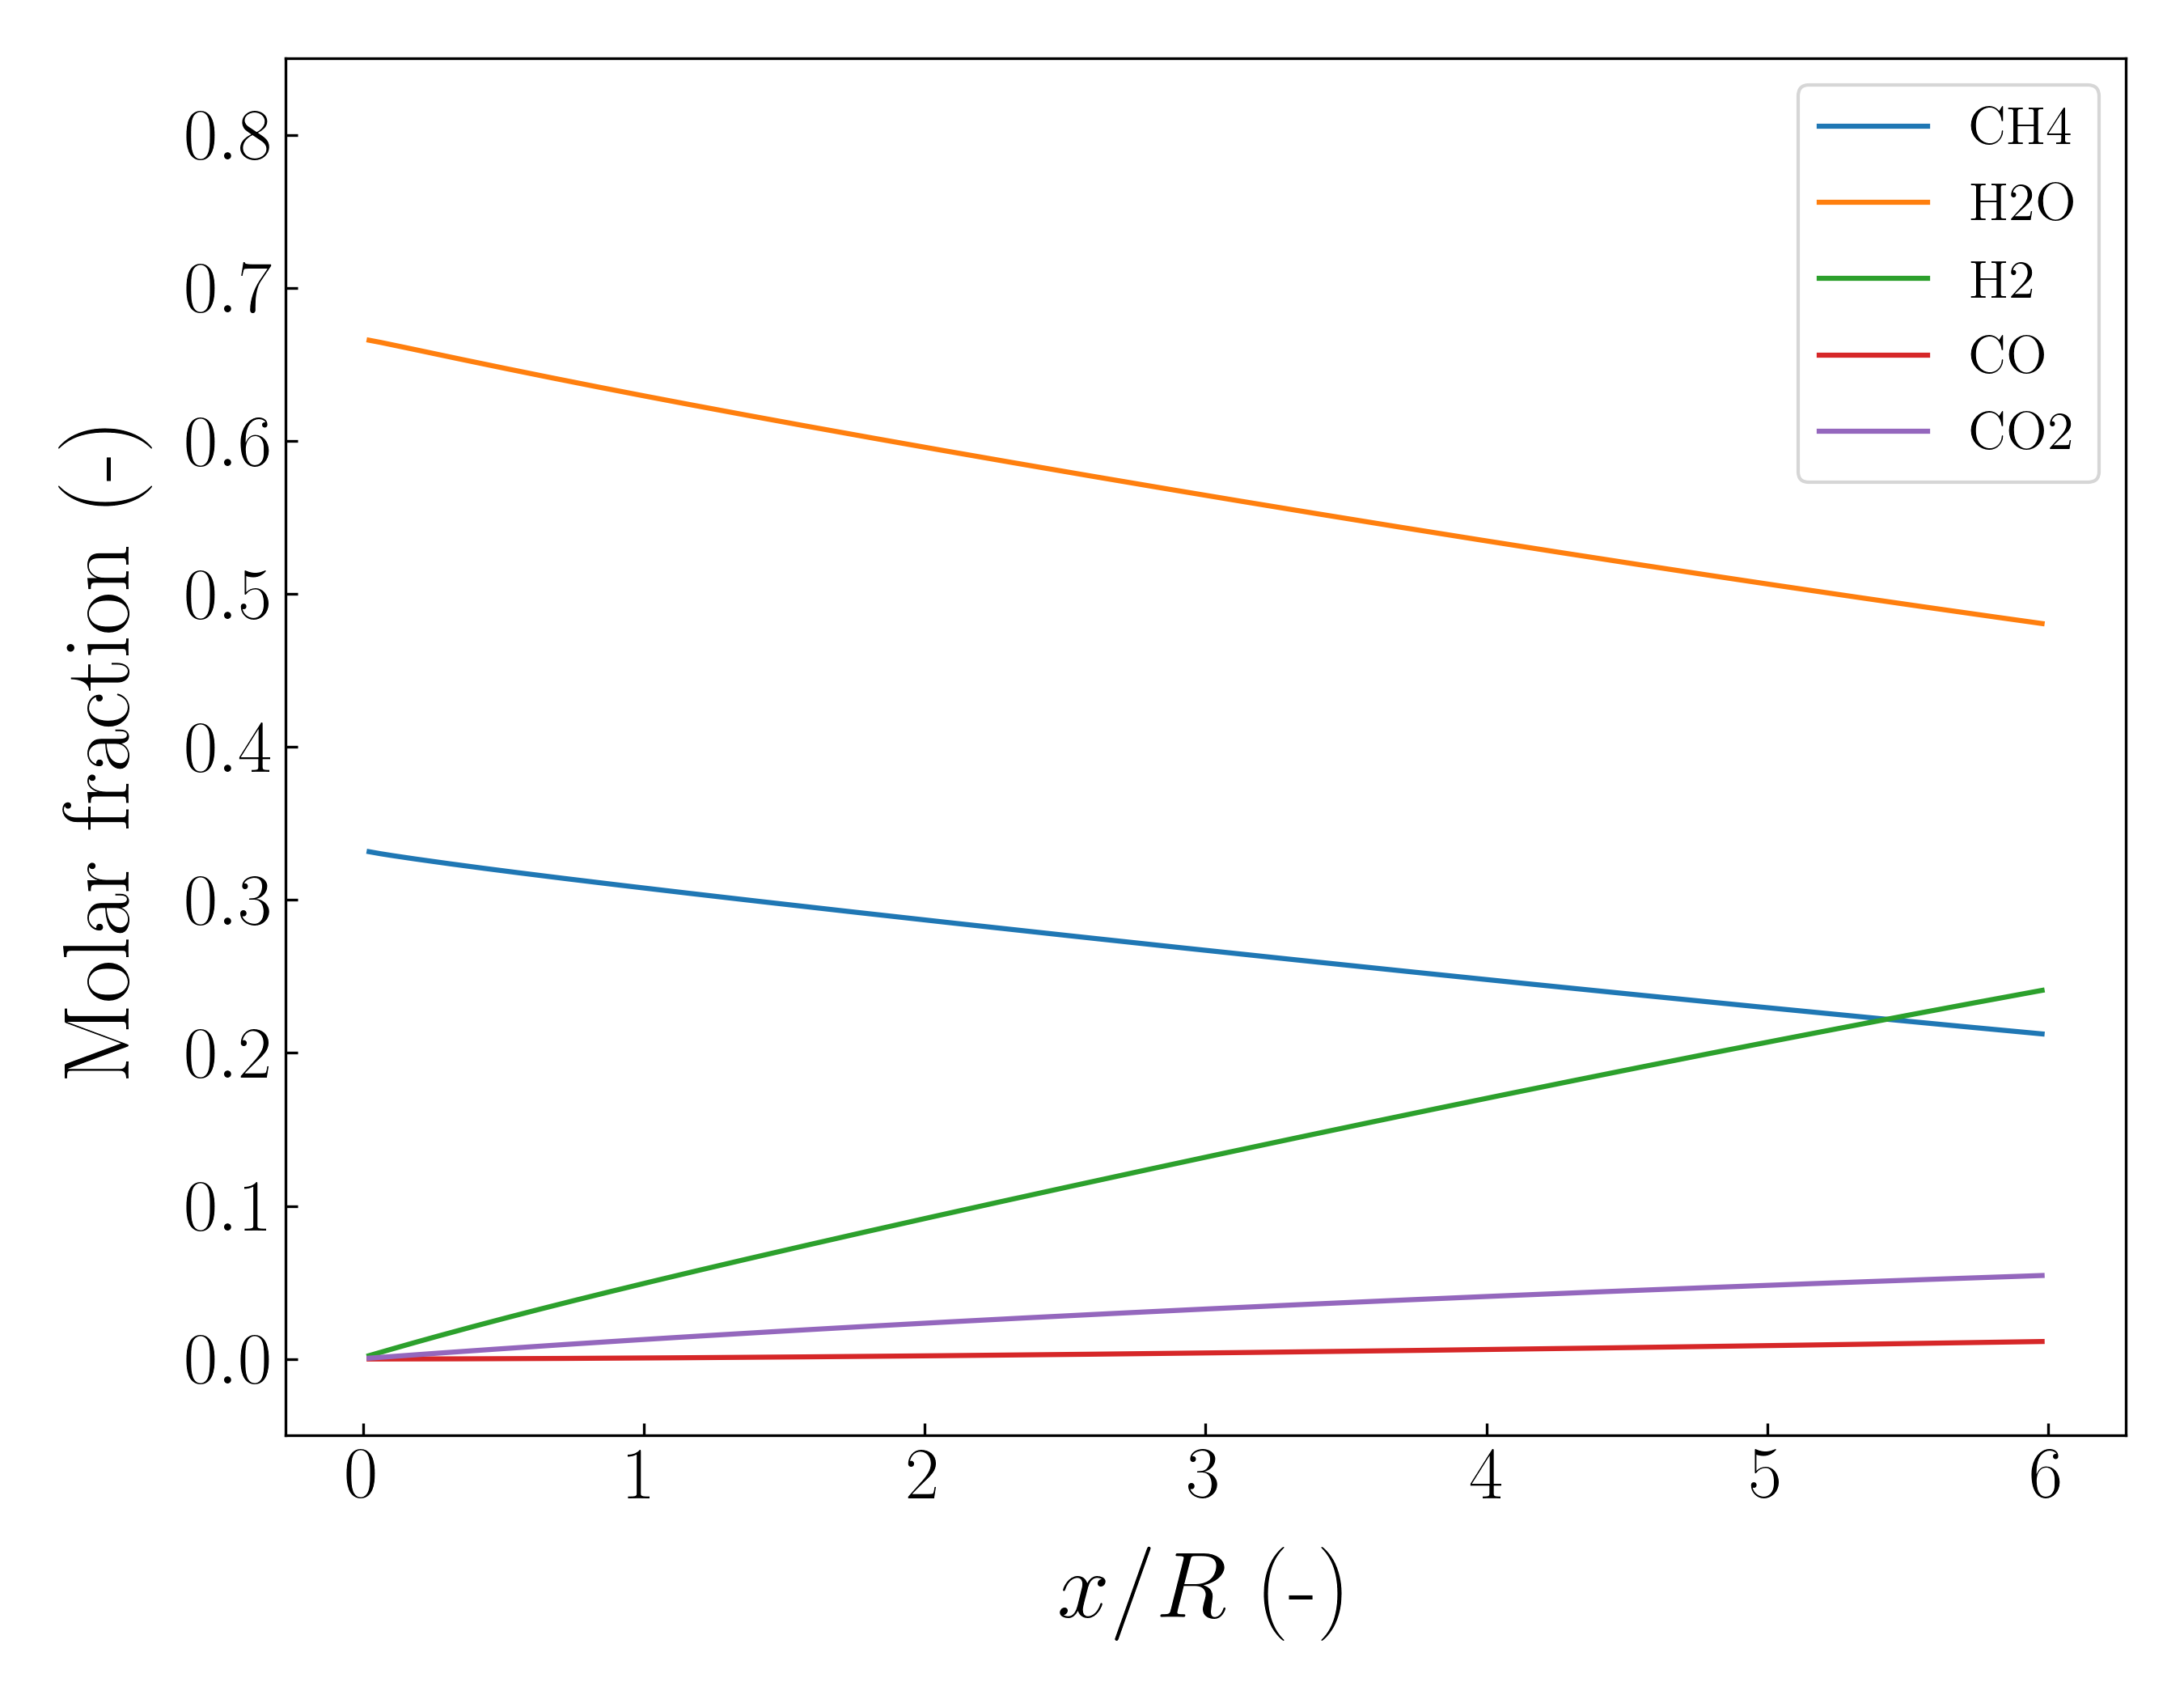
\includegraphics[width=80mm]{results/5/50C_50T/GEN1-AVG.png}
%\caption{\label{fig:5R5050G1-avg} Strategy I - Radius-averaged molar fractions - 1$^{\rm{st}}$ generation ($w_{\rm{CH_4}} = 0.5, w_T = 0.5$, $T_{\rm{in}}$ = 900 K, $u_{\rm{in}}$ = 0.15 m s$^{-1}$, $SC$ = 2.0)}
%\end{figure}
%
%\begin{figure}[h!]
%\centering
%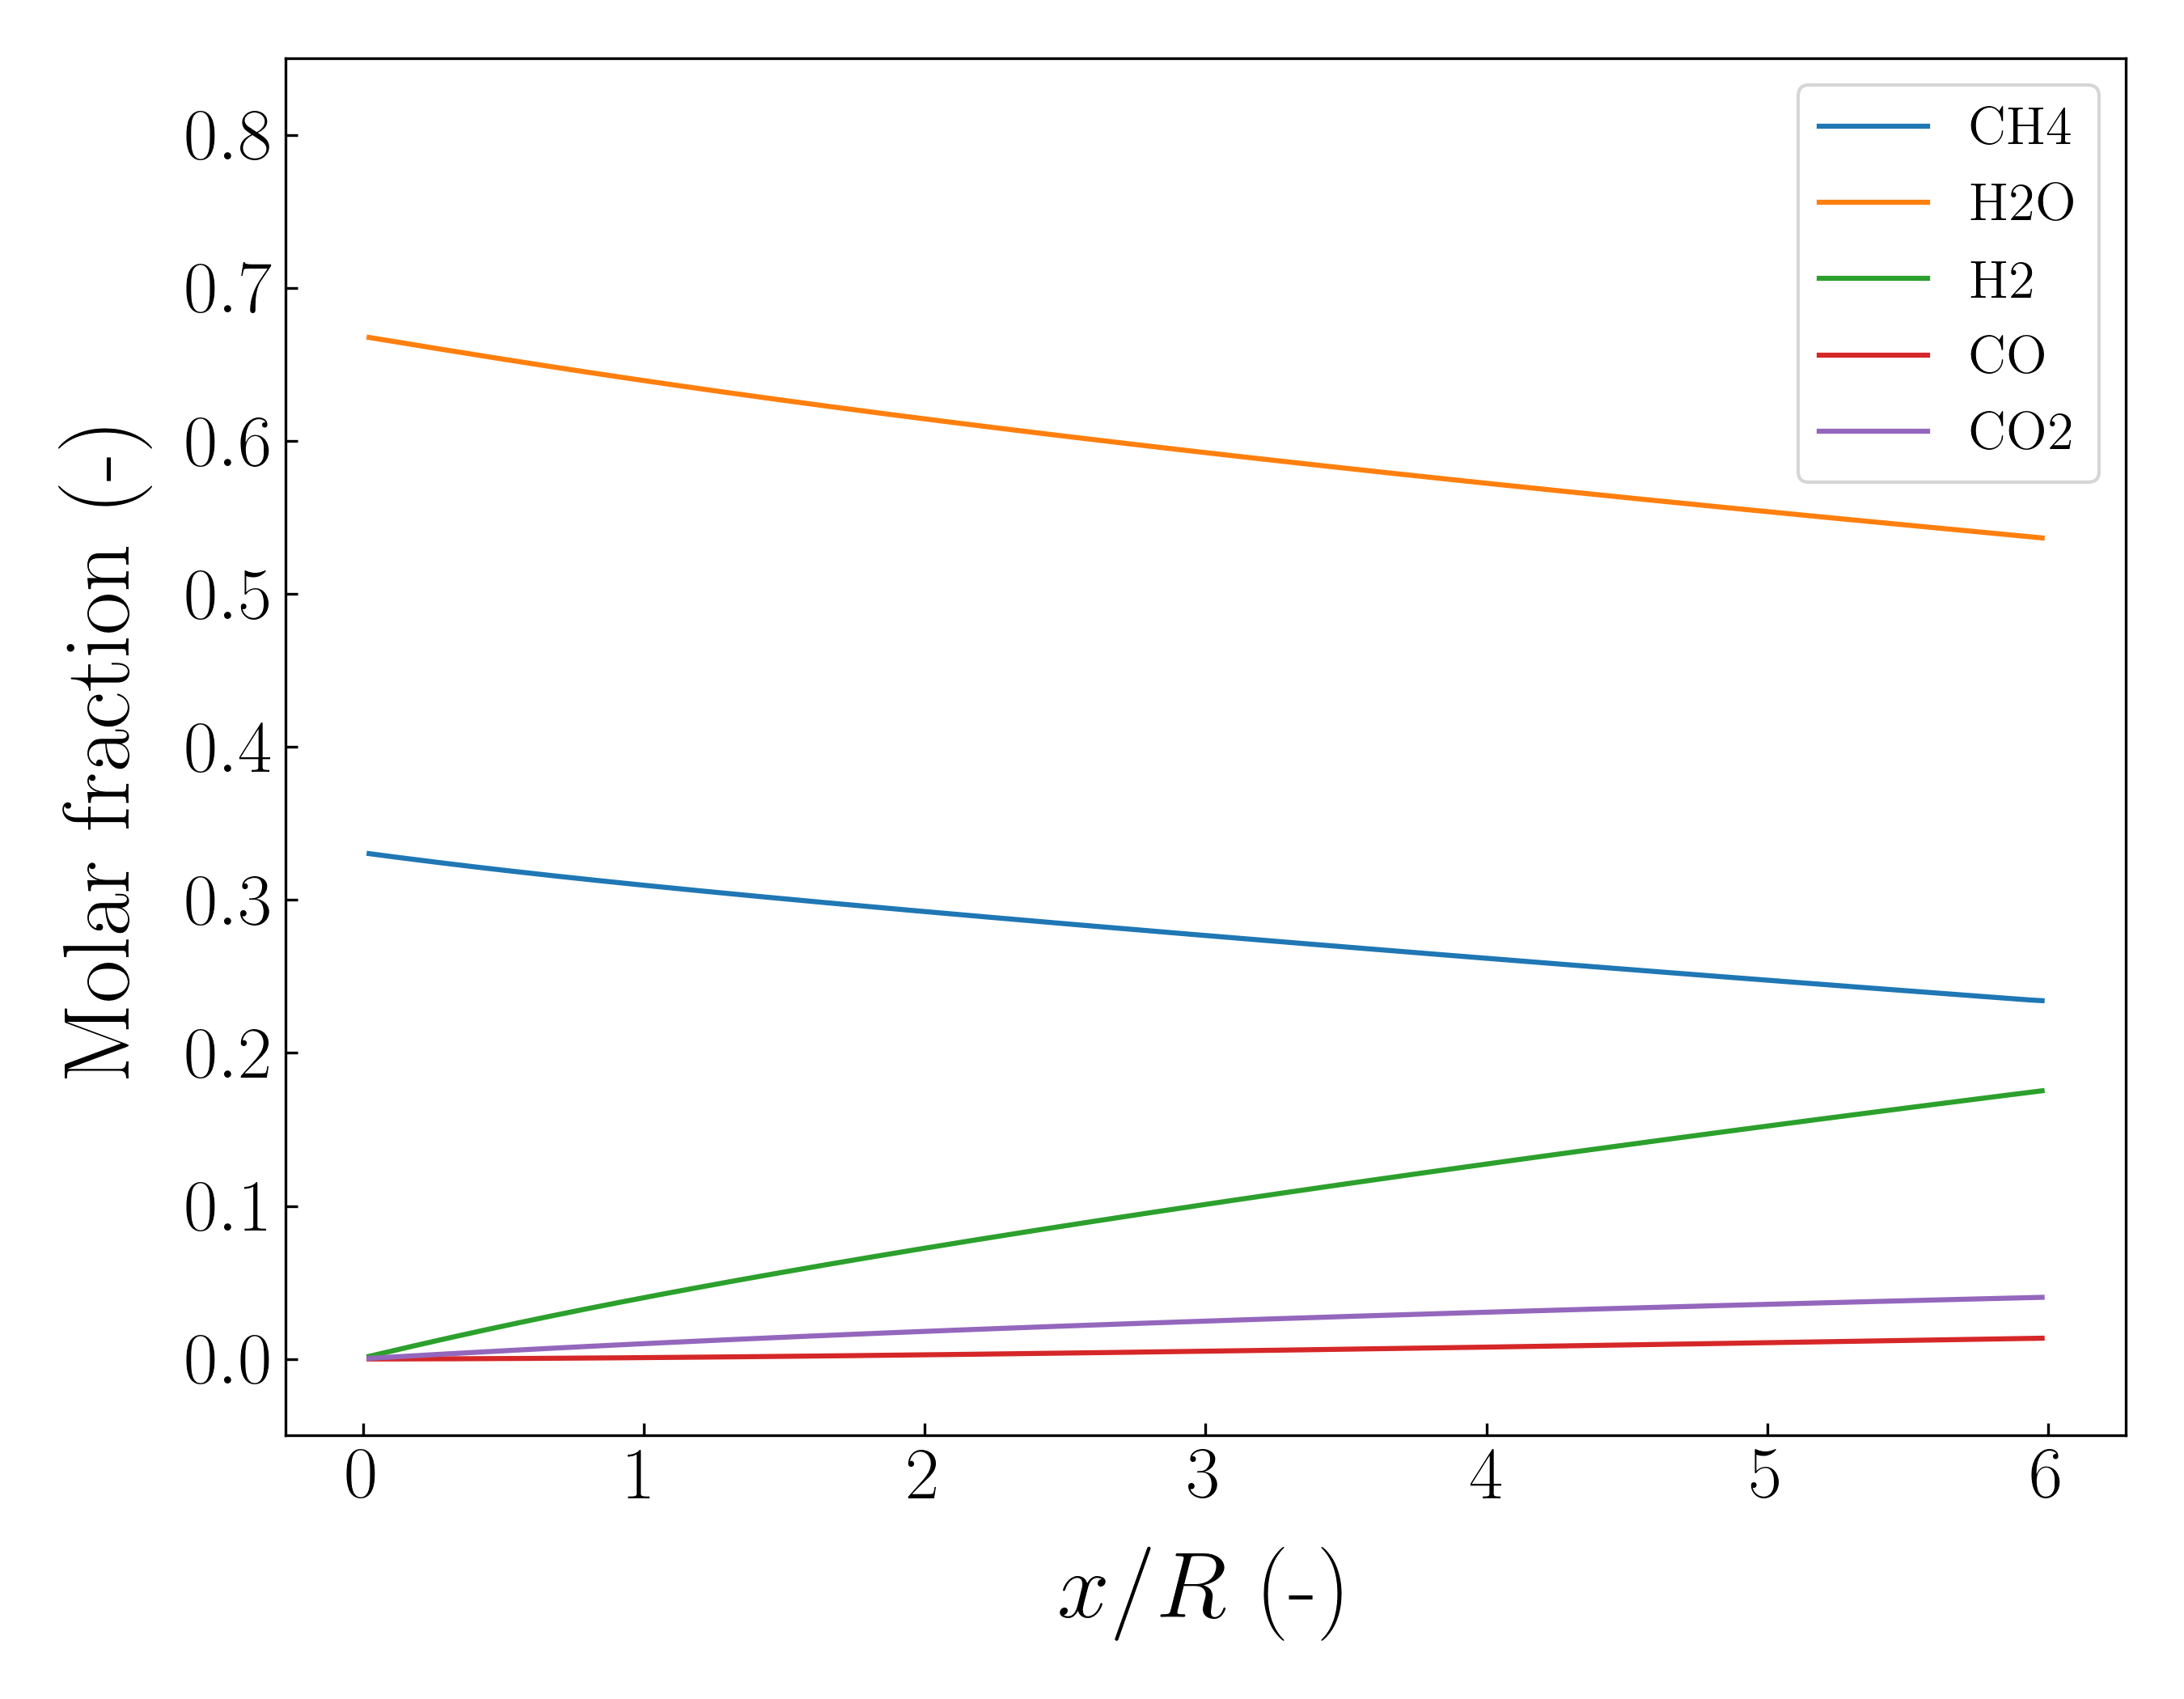
\includegraphics[width=80mm]{results/5/50C_50T/GEN15-AVG.png}
%\caption{\label{fig:5R5050G15-avg} Strategy I - Radius-averaged molar fractions - 15$^{\rm{th}}$ generation ($w_{\rm{CH_4}} = 0.5, w_T = 0.5$, $T_{\rm{in}}$ = 900 K, $u_{\rm{in}}$ = 0.15 m s$^{-1}$, $SC$ = 2.0)}
%\end{figure}
%
%\begin{figure}[h!]
%\centering
%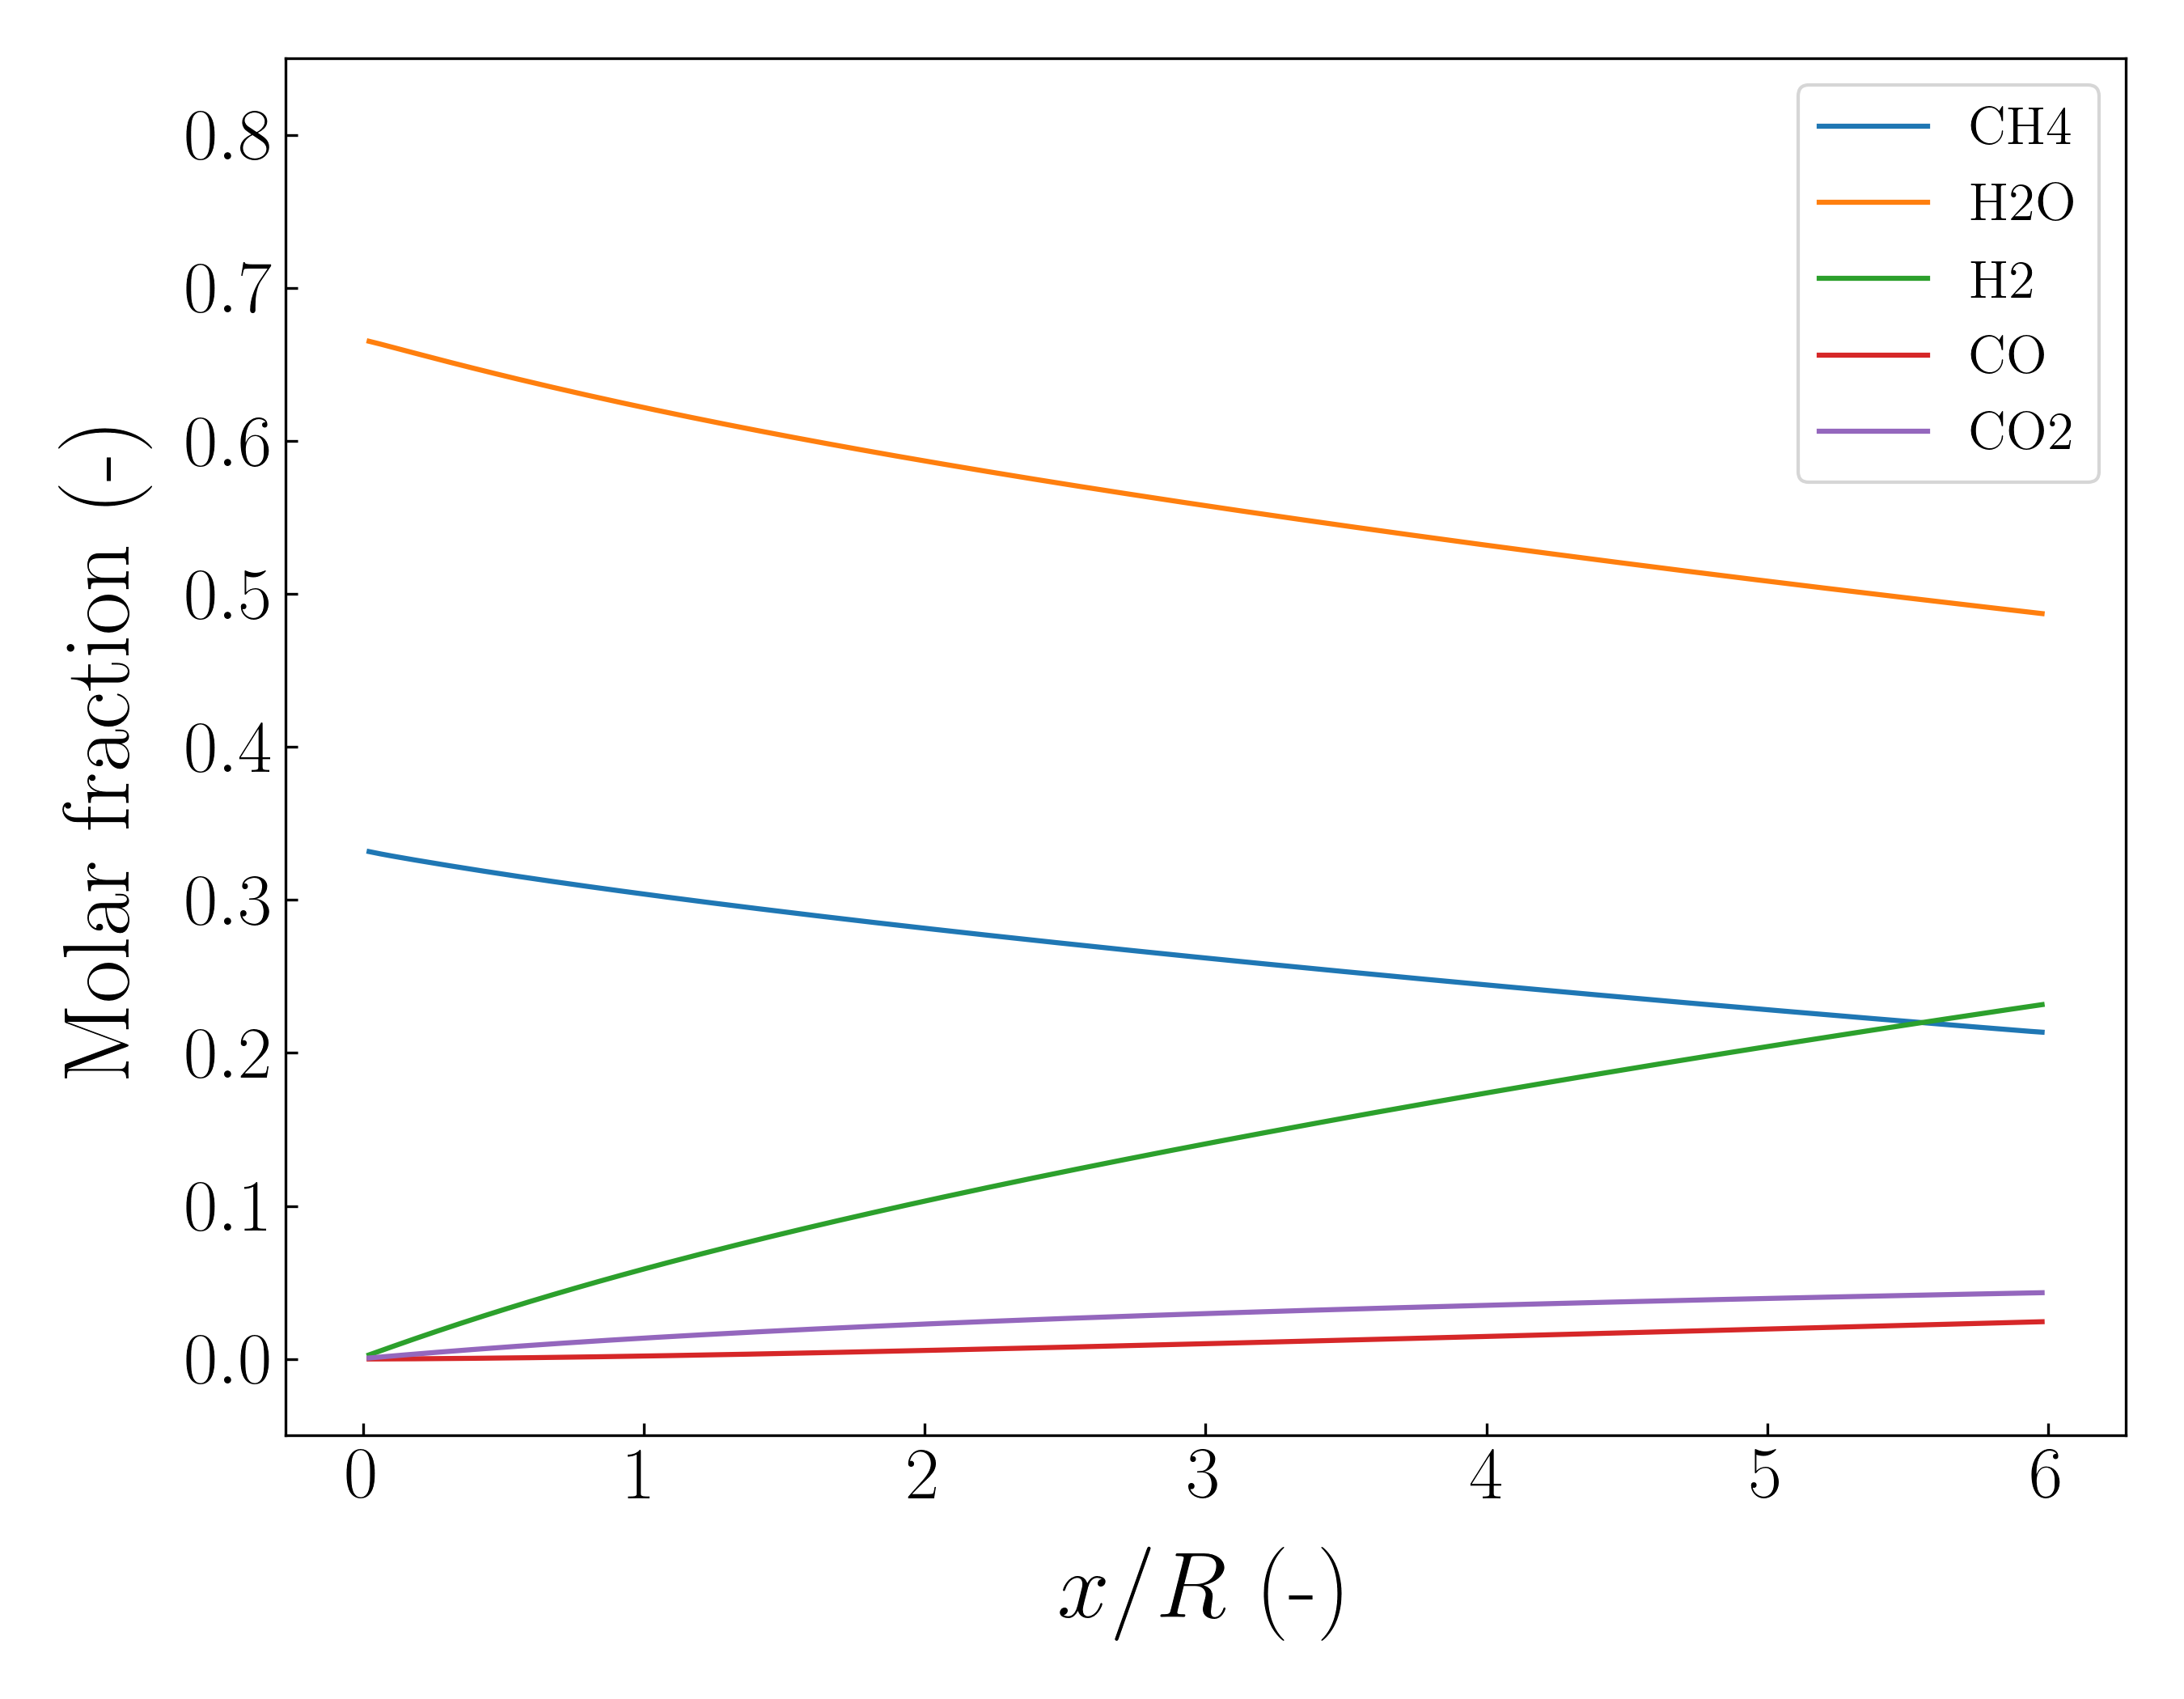
\includegraphics[width=80mm]{results/5/50C_50T/GEN30-AVG.png}
%\caption{\label{fig:5R5050G30-avg} Strategy I - Radius-averaged molar fractions -  30$^{\rm{th}}$ generation ($w_{\rm{CH_4}} = 0.5, w_T = 0.5$, $T_{\rm{in}}$ = 900 K, $u_{\rm{in}}$ = 0.15 m s$^{-1}$, $SC$ = 2.0)}
%\end{figure}
%
%\begin{figure}[h!]
%\centering
%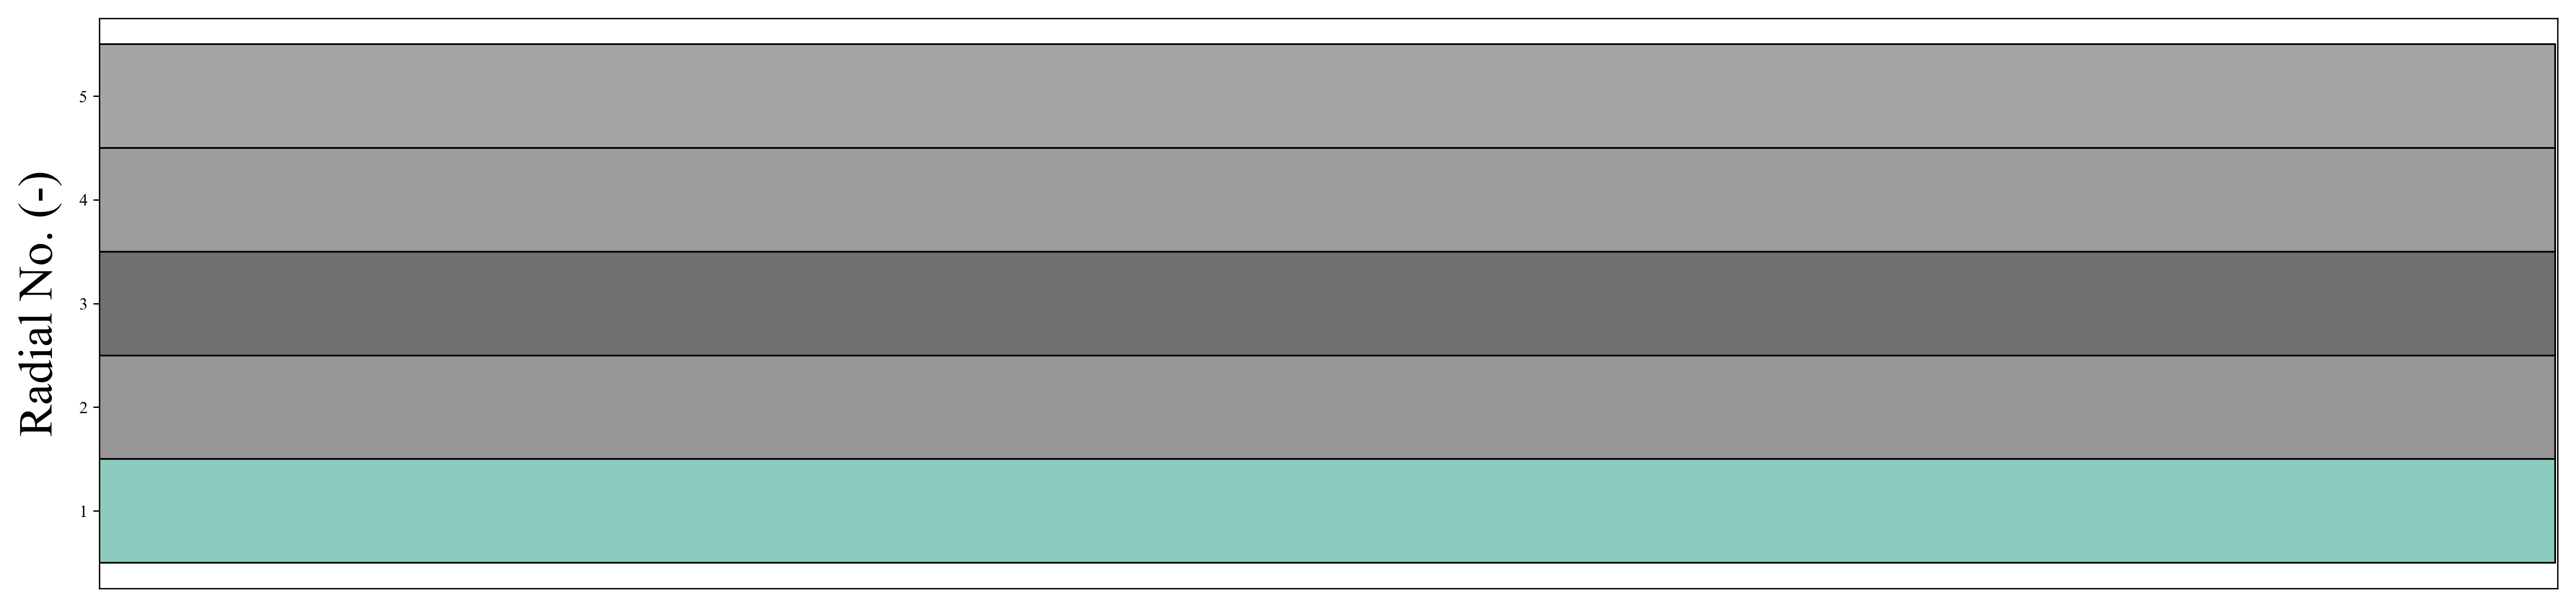
\includegraphics[width=120mm]{results/segments/5seg/50C50T/seg.png}
%\caption{\label{fig:30L6040G1-TField} Strategy I - Segments distribution for 30$^{\rm{th}}$ generation ($w_{\rm{CH_4}} = 0.5, w_T = 0.5$, $T_{\rm{in}}$ = 900 K, $u_{\rm{in}}$ = 0.15 m s$^{-1}$, $SC$ = 2.0)}
%\end{figure}
%
%\begin{figure}[h!]
%\centering
%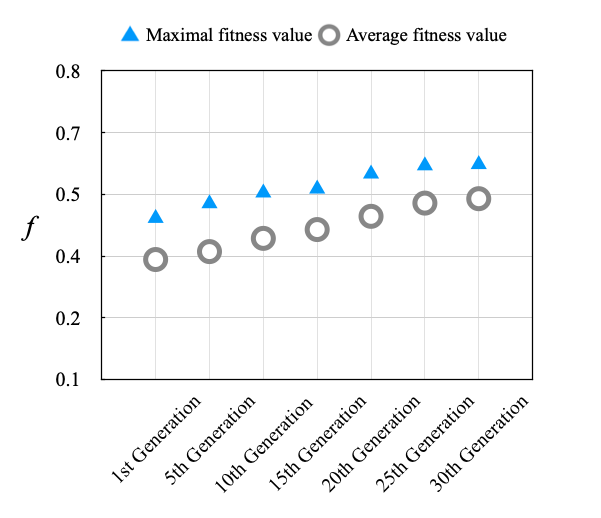
\includegraphics[width=100mm]{results/5/50C_50T.png}
%\caption{\label{fig:5R5050G-fitness} Strategy I - Fitness analysis throughout successive populations ($w_{\rm{CH_4}} = 0.5, w_T = 0.5$, $T_{\rm{in}}$ = 900 K, $u_{\rm{in}}$ = 0.15 m s$^{-1}$, $SC$ = 2.0)}
%\end{figure}
%
%
%\clearpage
%
%
%
%\paragraph{Thermal fitness 40 \%, methane conversion 60 \%} \hspace{0pt} \\
%\noindent 
%
%
%\begin{figure}[h!]
%\centering
%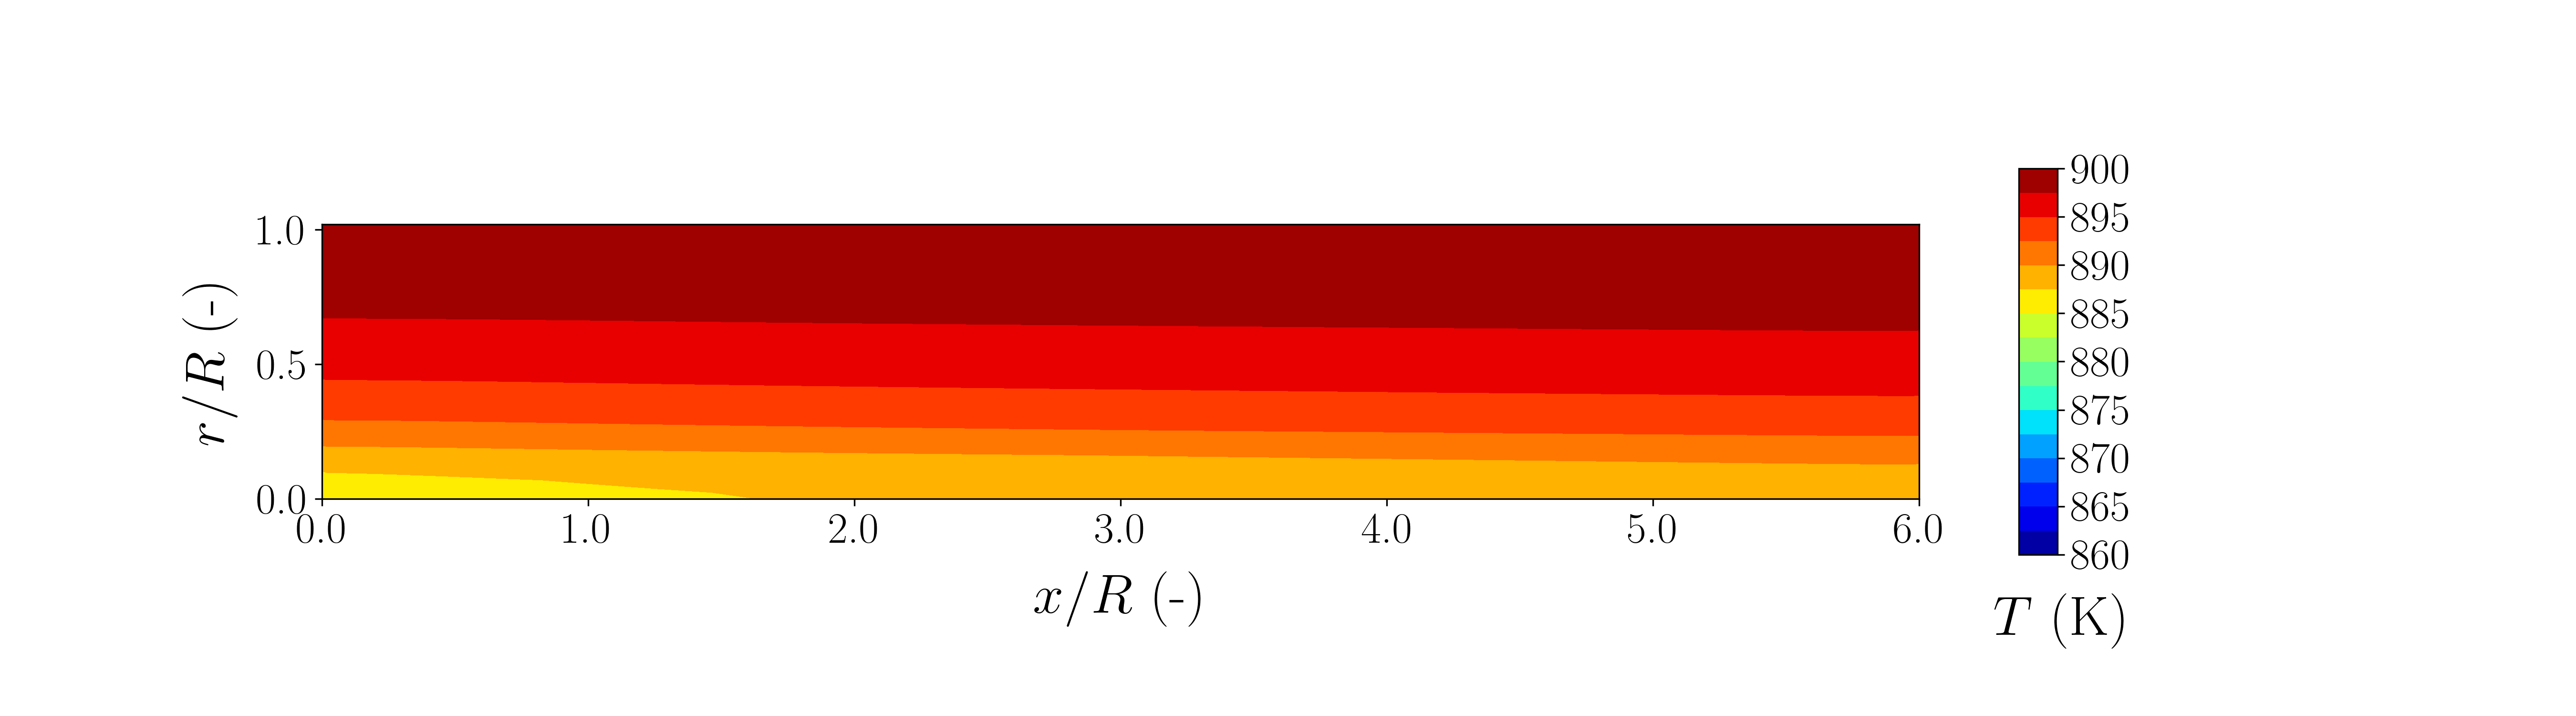
\includegraphics[width=190mm]{results/5/60C_40T/GEN1-TFIELD.png}
%\caption{\label{fig:5R6040G1-TField} Strategy I - Temperature field distribution - 1$^{\rm{st}}$ generation ($w_{\rm{CH_4}} = 0.6, w_T = 0.4$, $T_{\rm{in}}$ = 900 K, $u_{\rm{in}}$ = 0.15 m s$^{-1}$, $SC$ = 2.0)}
%\end{figure}
%
%\begin{figure}[h!]
%\centering
%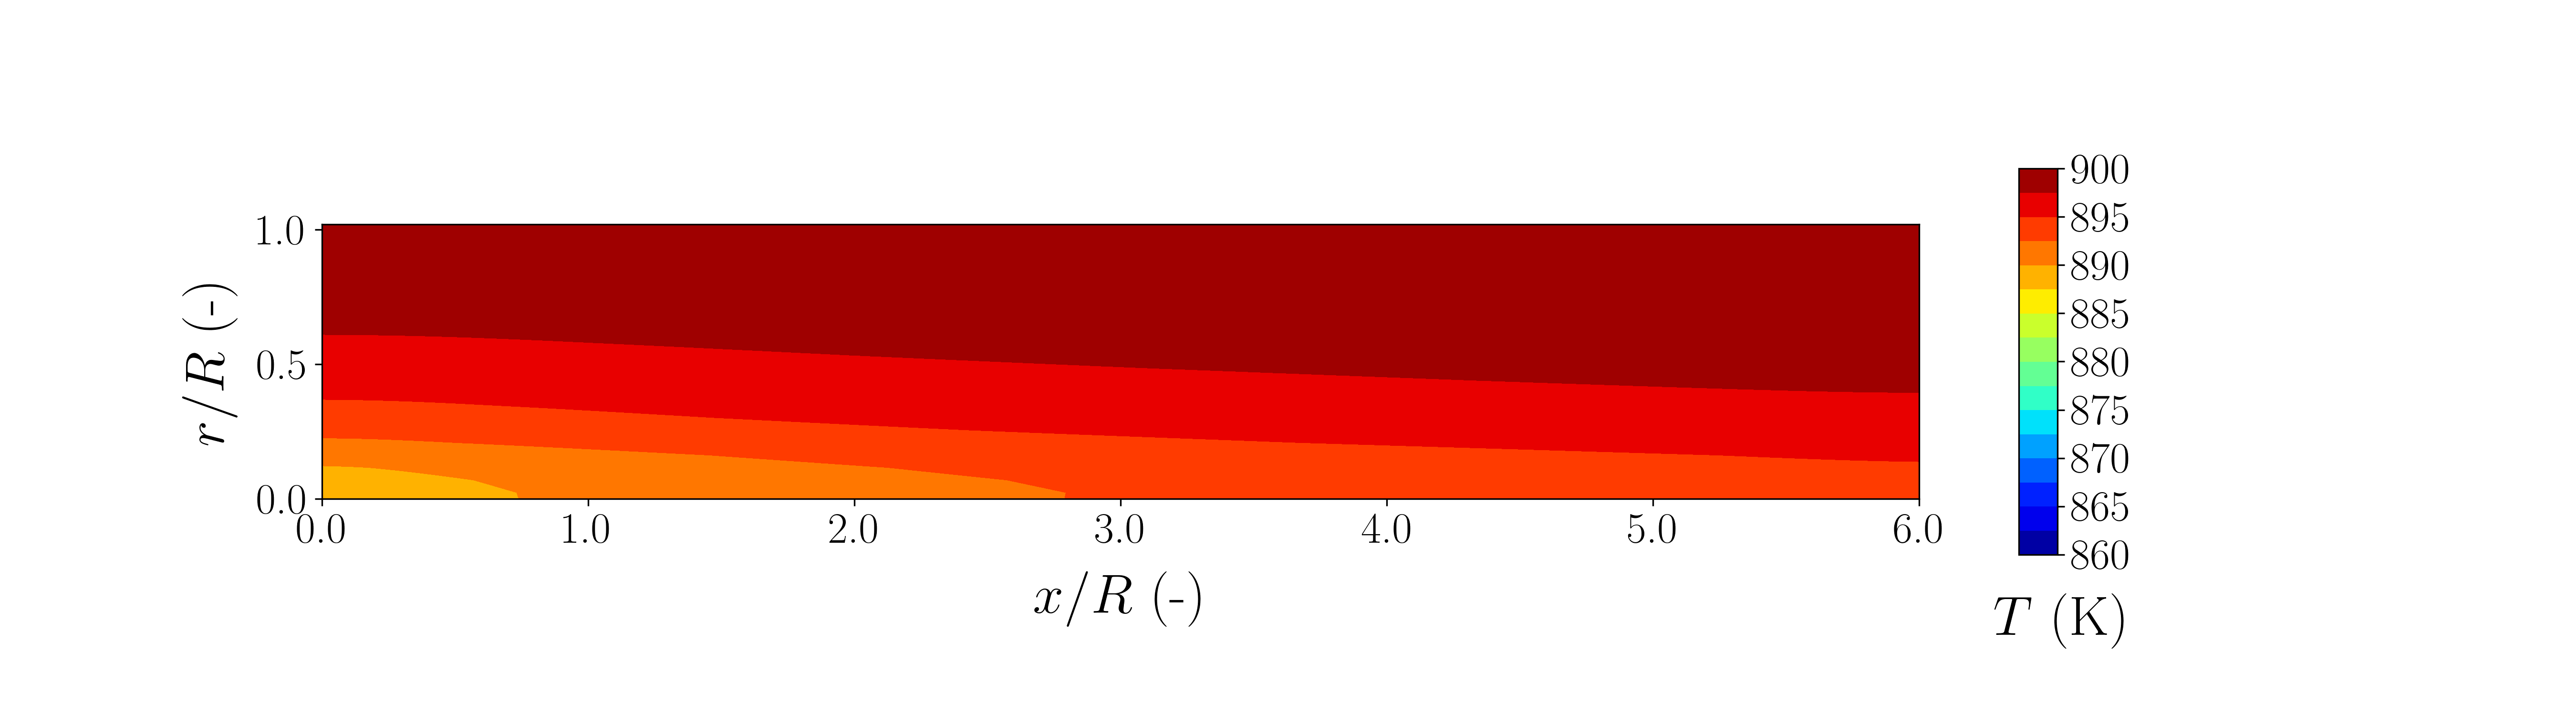
\includegraphics[width=190mm]{results/5/60C_40T/GEN15-TFIELD.png}
%\caption{\label{fig:5R6040G15-TField} Strategy I - Temperature field distribution - 15$^{\rm{th}}$ generation ($w_{\rm{CH_4}} = 0.6, w_T = 0.4$, $T_{\rm{in}}$ = 900 K, $u_{\rm{in}}$ = 0.15 m s$^{-1}$, $SC$ = 2.0)}
%\end{figure}
%
%\begin{figure}[h!]
%\centering
%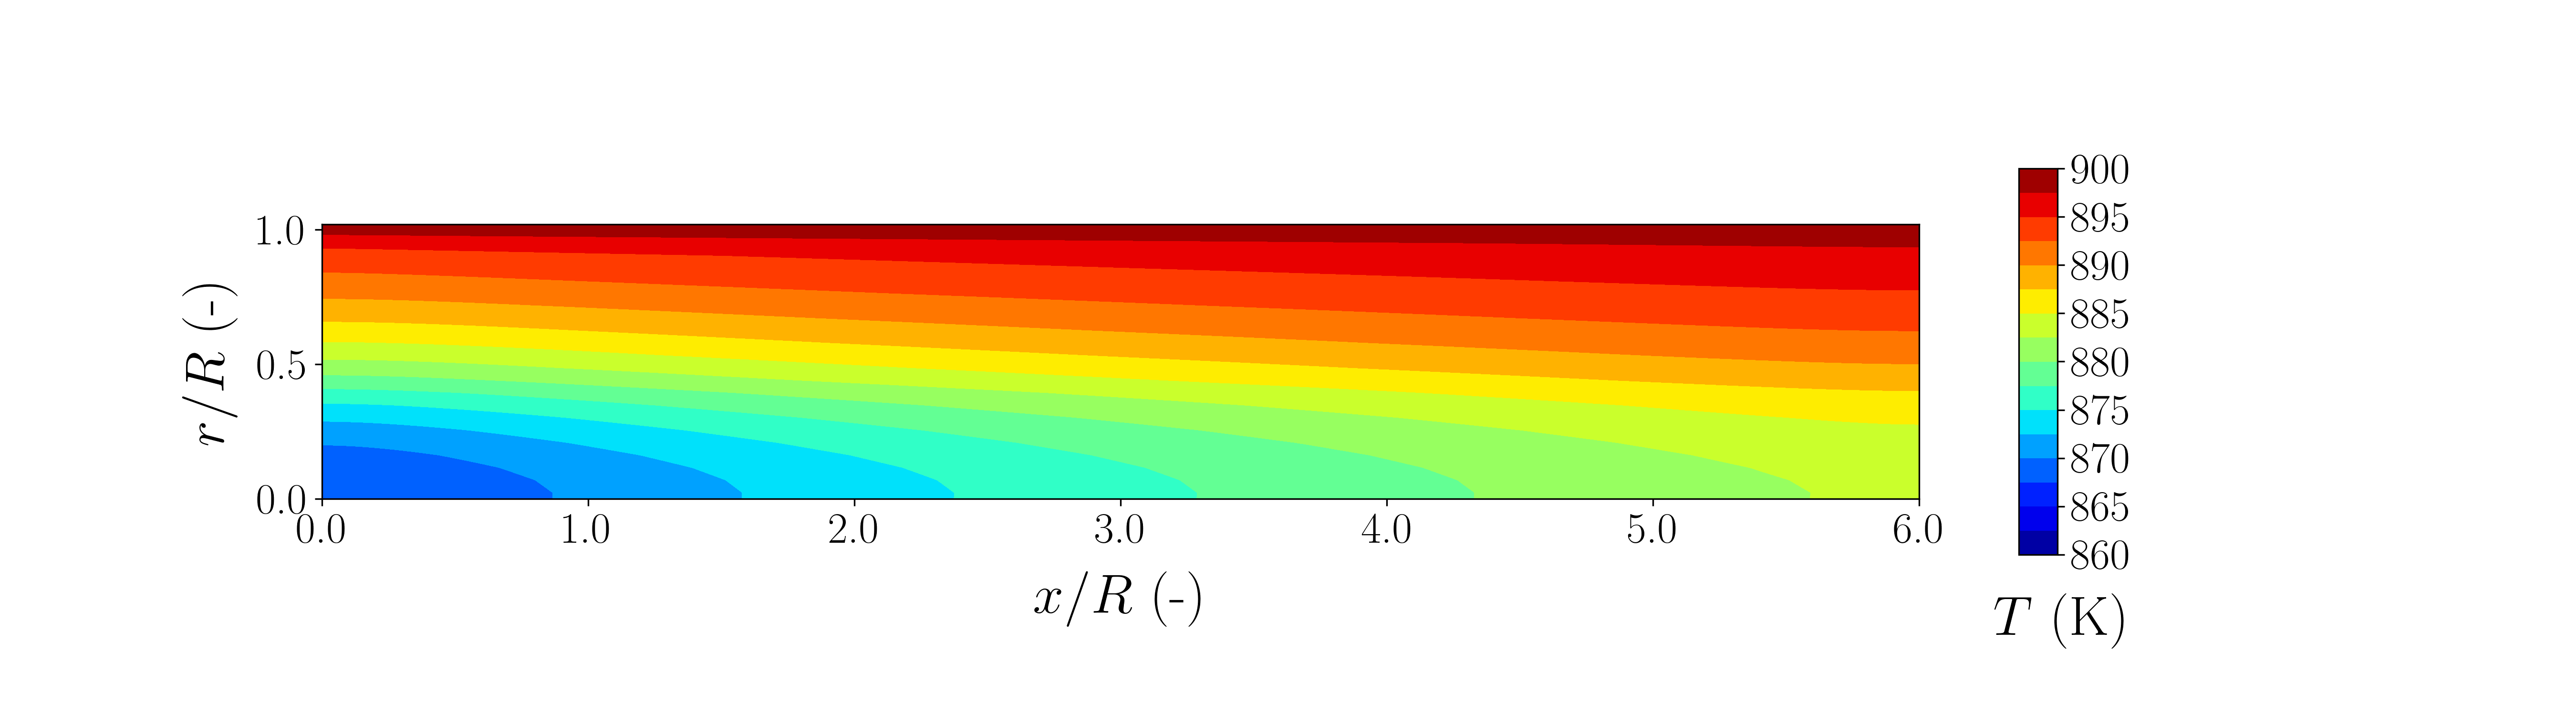
\includegraphics[width=190mm]{results/5/60C_40T/GEN30-TFIELD.png}
%\caption{\label{fig:5R6040G30-TField} Strategy I - Temperature field distribution - 30$^{\rm{th}}$ generation ($w_{\rm{CH_4}} = 0.6, w_T = 0.4$, $T_{\rm{in}}$ = 900 K, $u_{\rm{in}}$ = 0.15 m s$^{-1}$, $SC$ = 2.0)}
%\end{figure}
%
%
%\begin{figure}[h!]
%\centering
%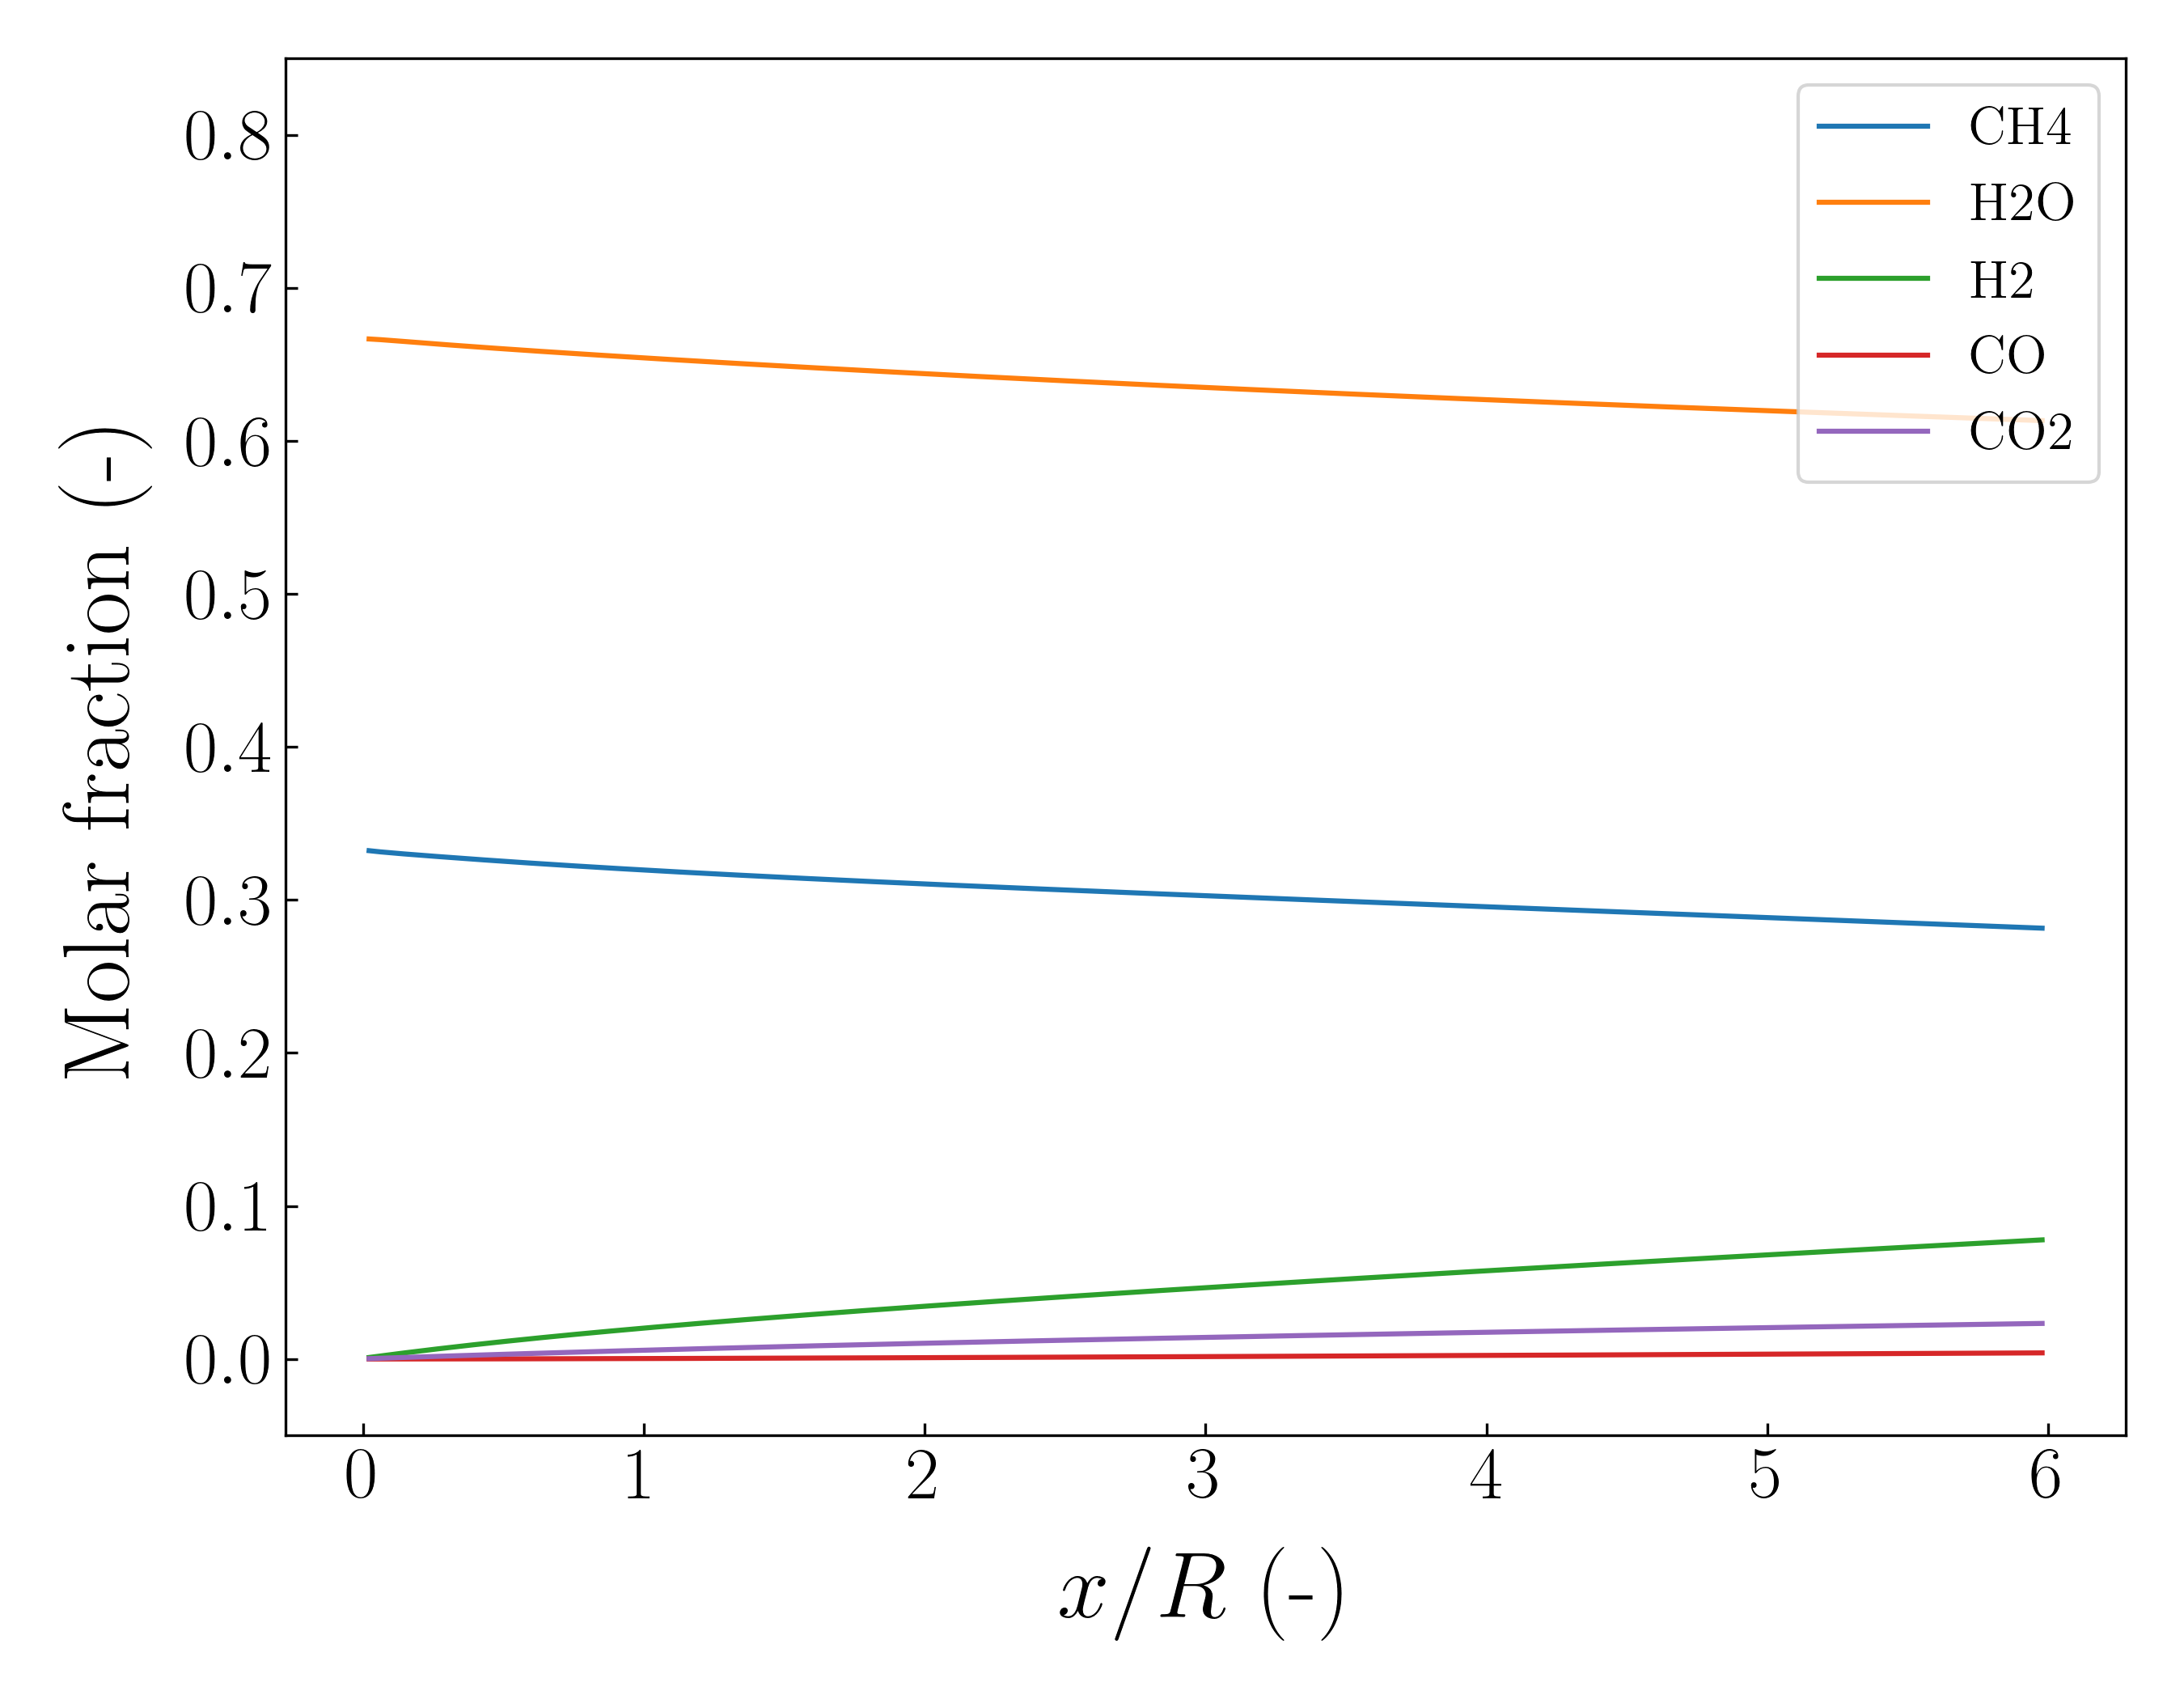
\includegraphics[width=80mm]{results/5/60C_40T/GEN1-AVG.png}
%\caption{\label{fig:5R6040G1-avg} Strategy I - Radius-averaged molar fractions - 1$^{\rm{st}}$ generation ($w_{\rm{CH_4}} = 0.6, w_T = 0.4$, $T_{\rm{in}}$ = 900 K, $u_{\rm{in}}$ = 0.15 m s$^{-1}$, $SC$ = 2.0)}
%\end{figure}
%
%\begin{figure}[h!]
%\centering
%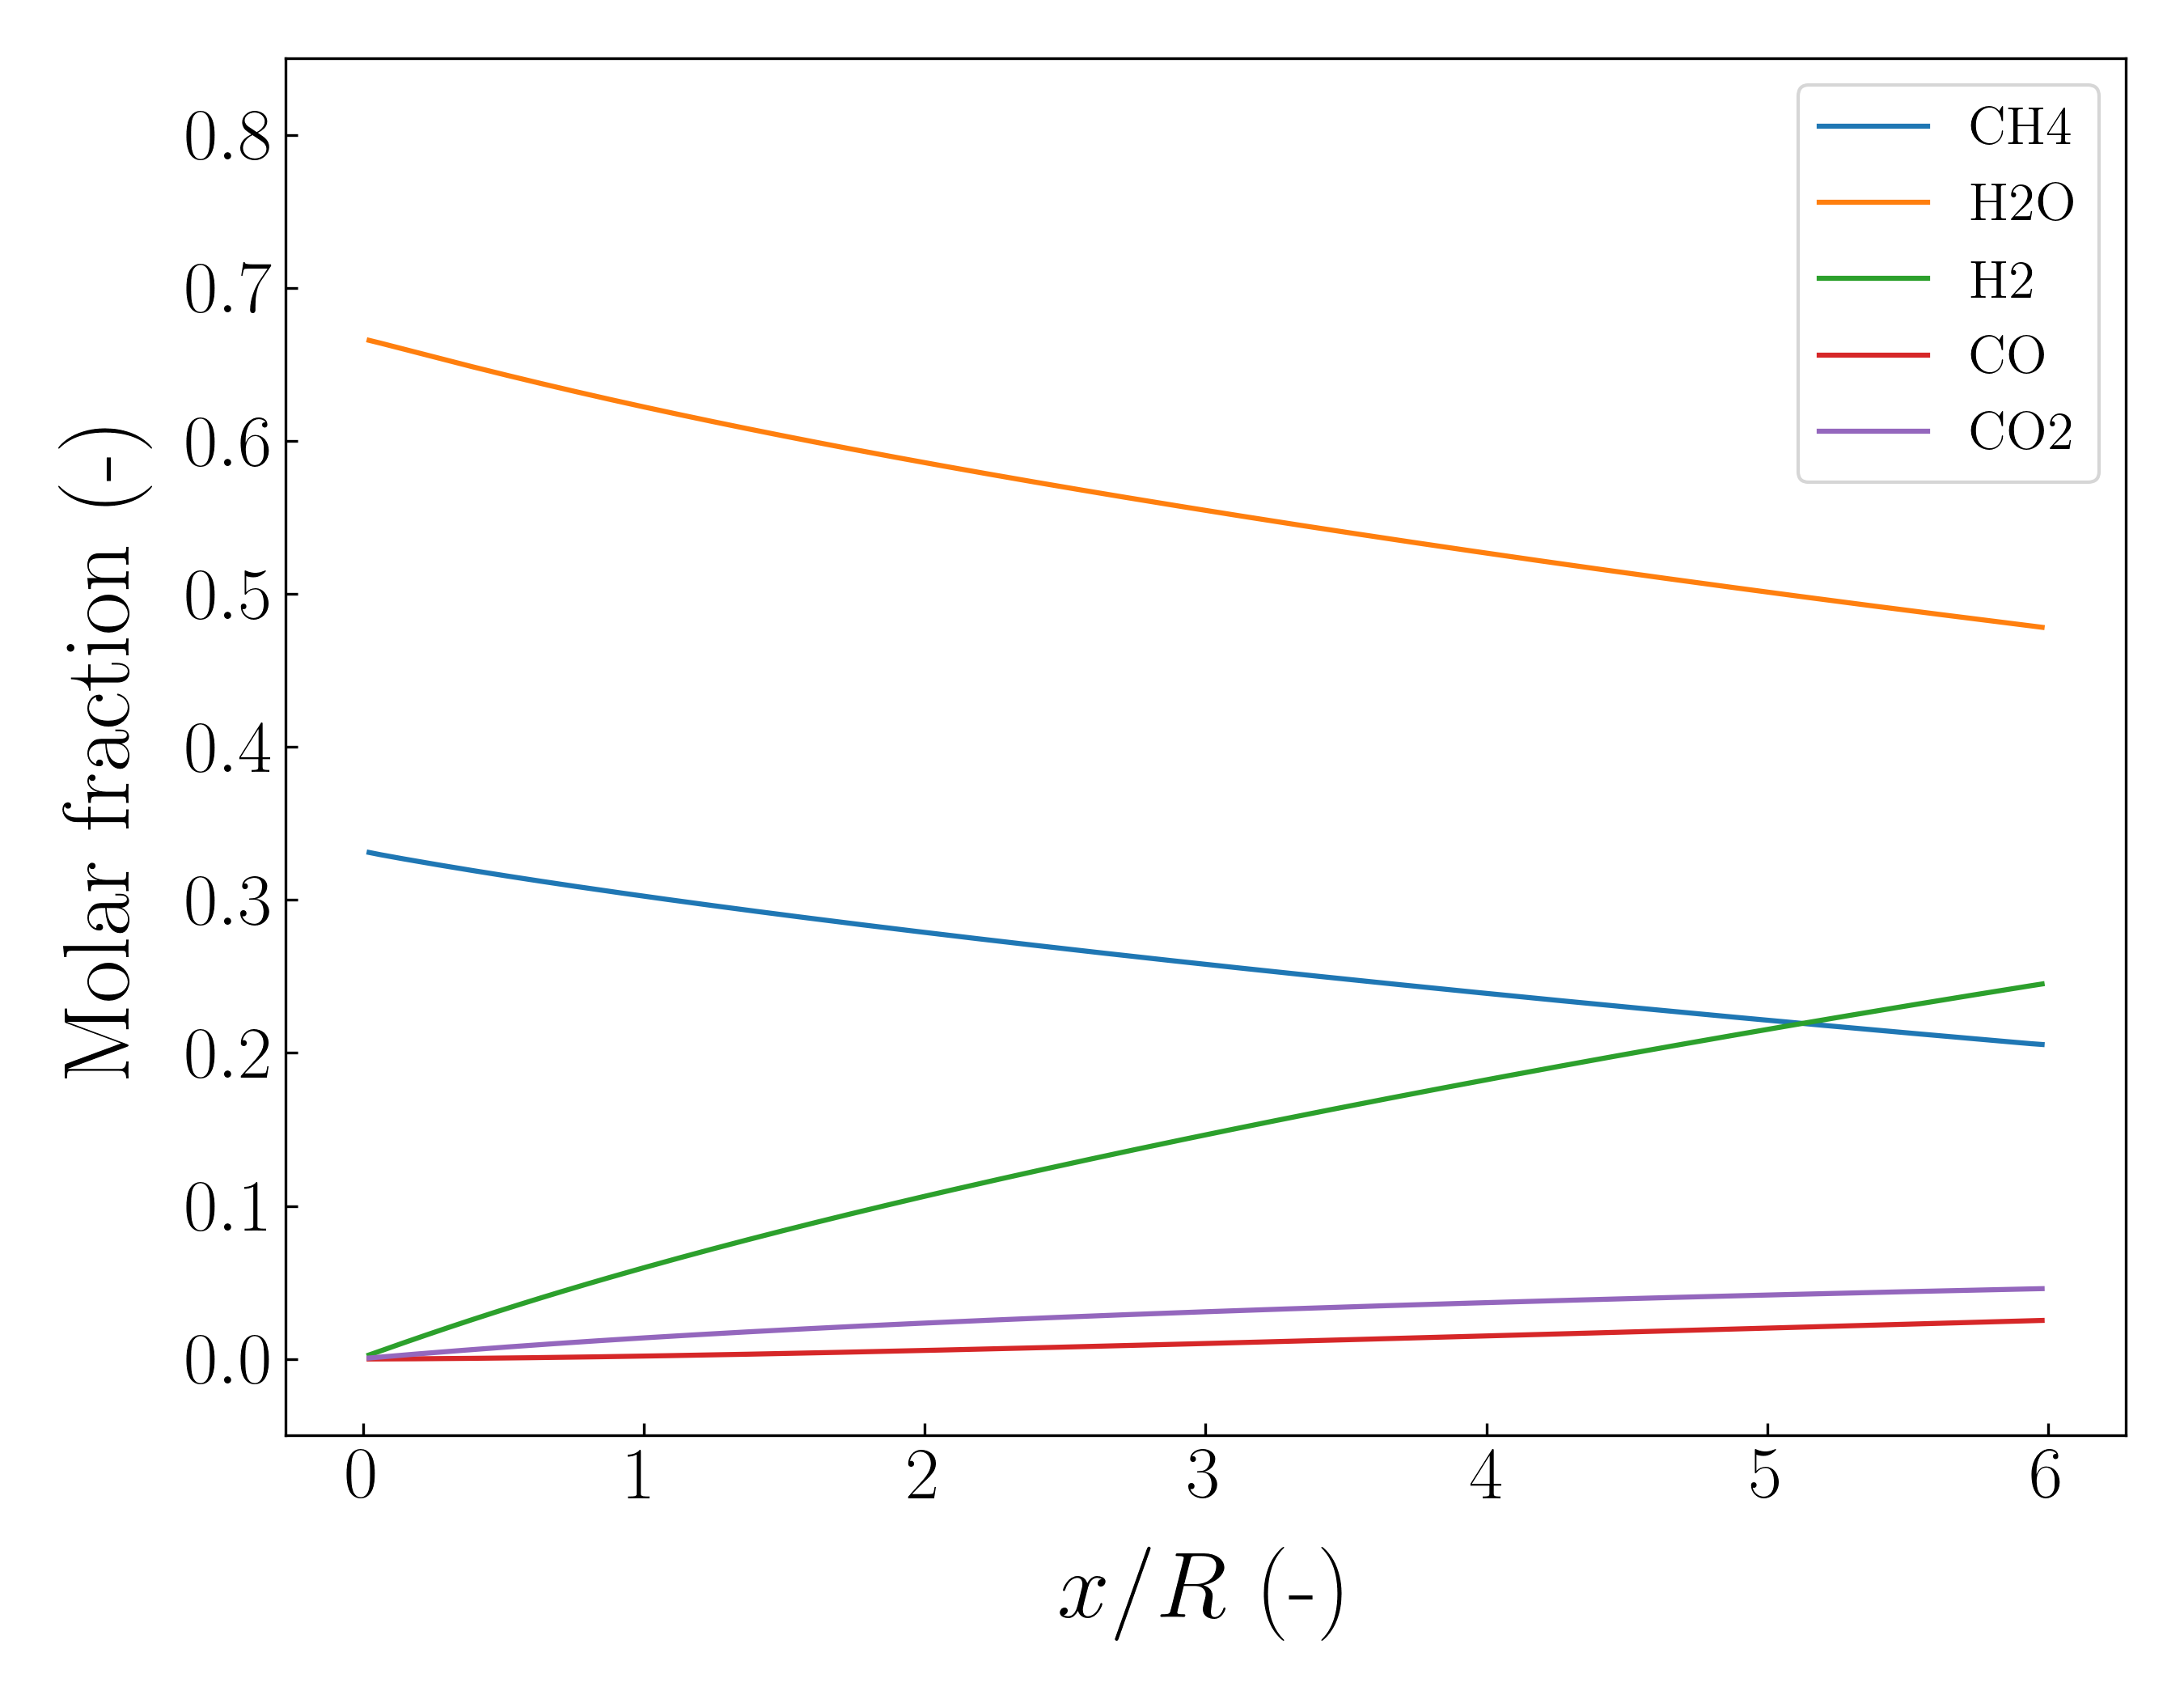
\includegraphics[width=80mm]{results/5/60C_40T/GEN15-AVG.png}
%\caption{\label{fig:5R6040G15-avg} Strategy I - Radius-averaged molar fractions - 15$^{\rm{th}}$ generation ($w_{\rm{CH_4}} = 0.6, w_T = 0.4$, $T_{\rm{in}}$ = 900 K, $u_{\rm{in}}$ = 0.15 m s$^{-1}$, $SC$ = 2.0)}
%\end{figure}
%
%\begin{figure}[h!]
%\centering
%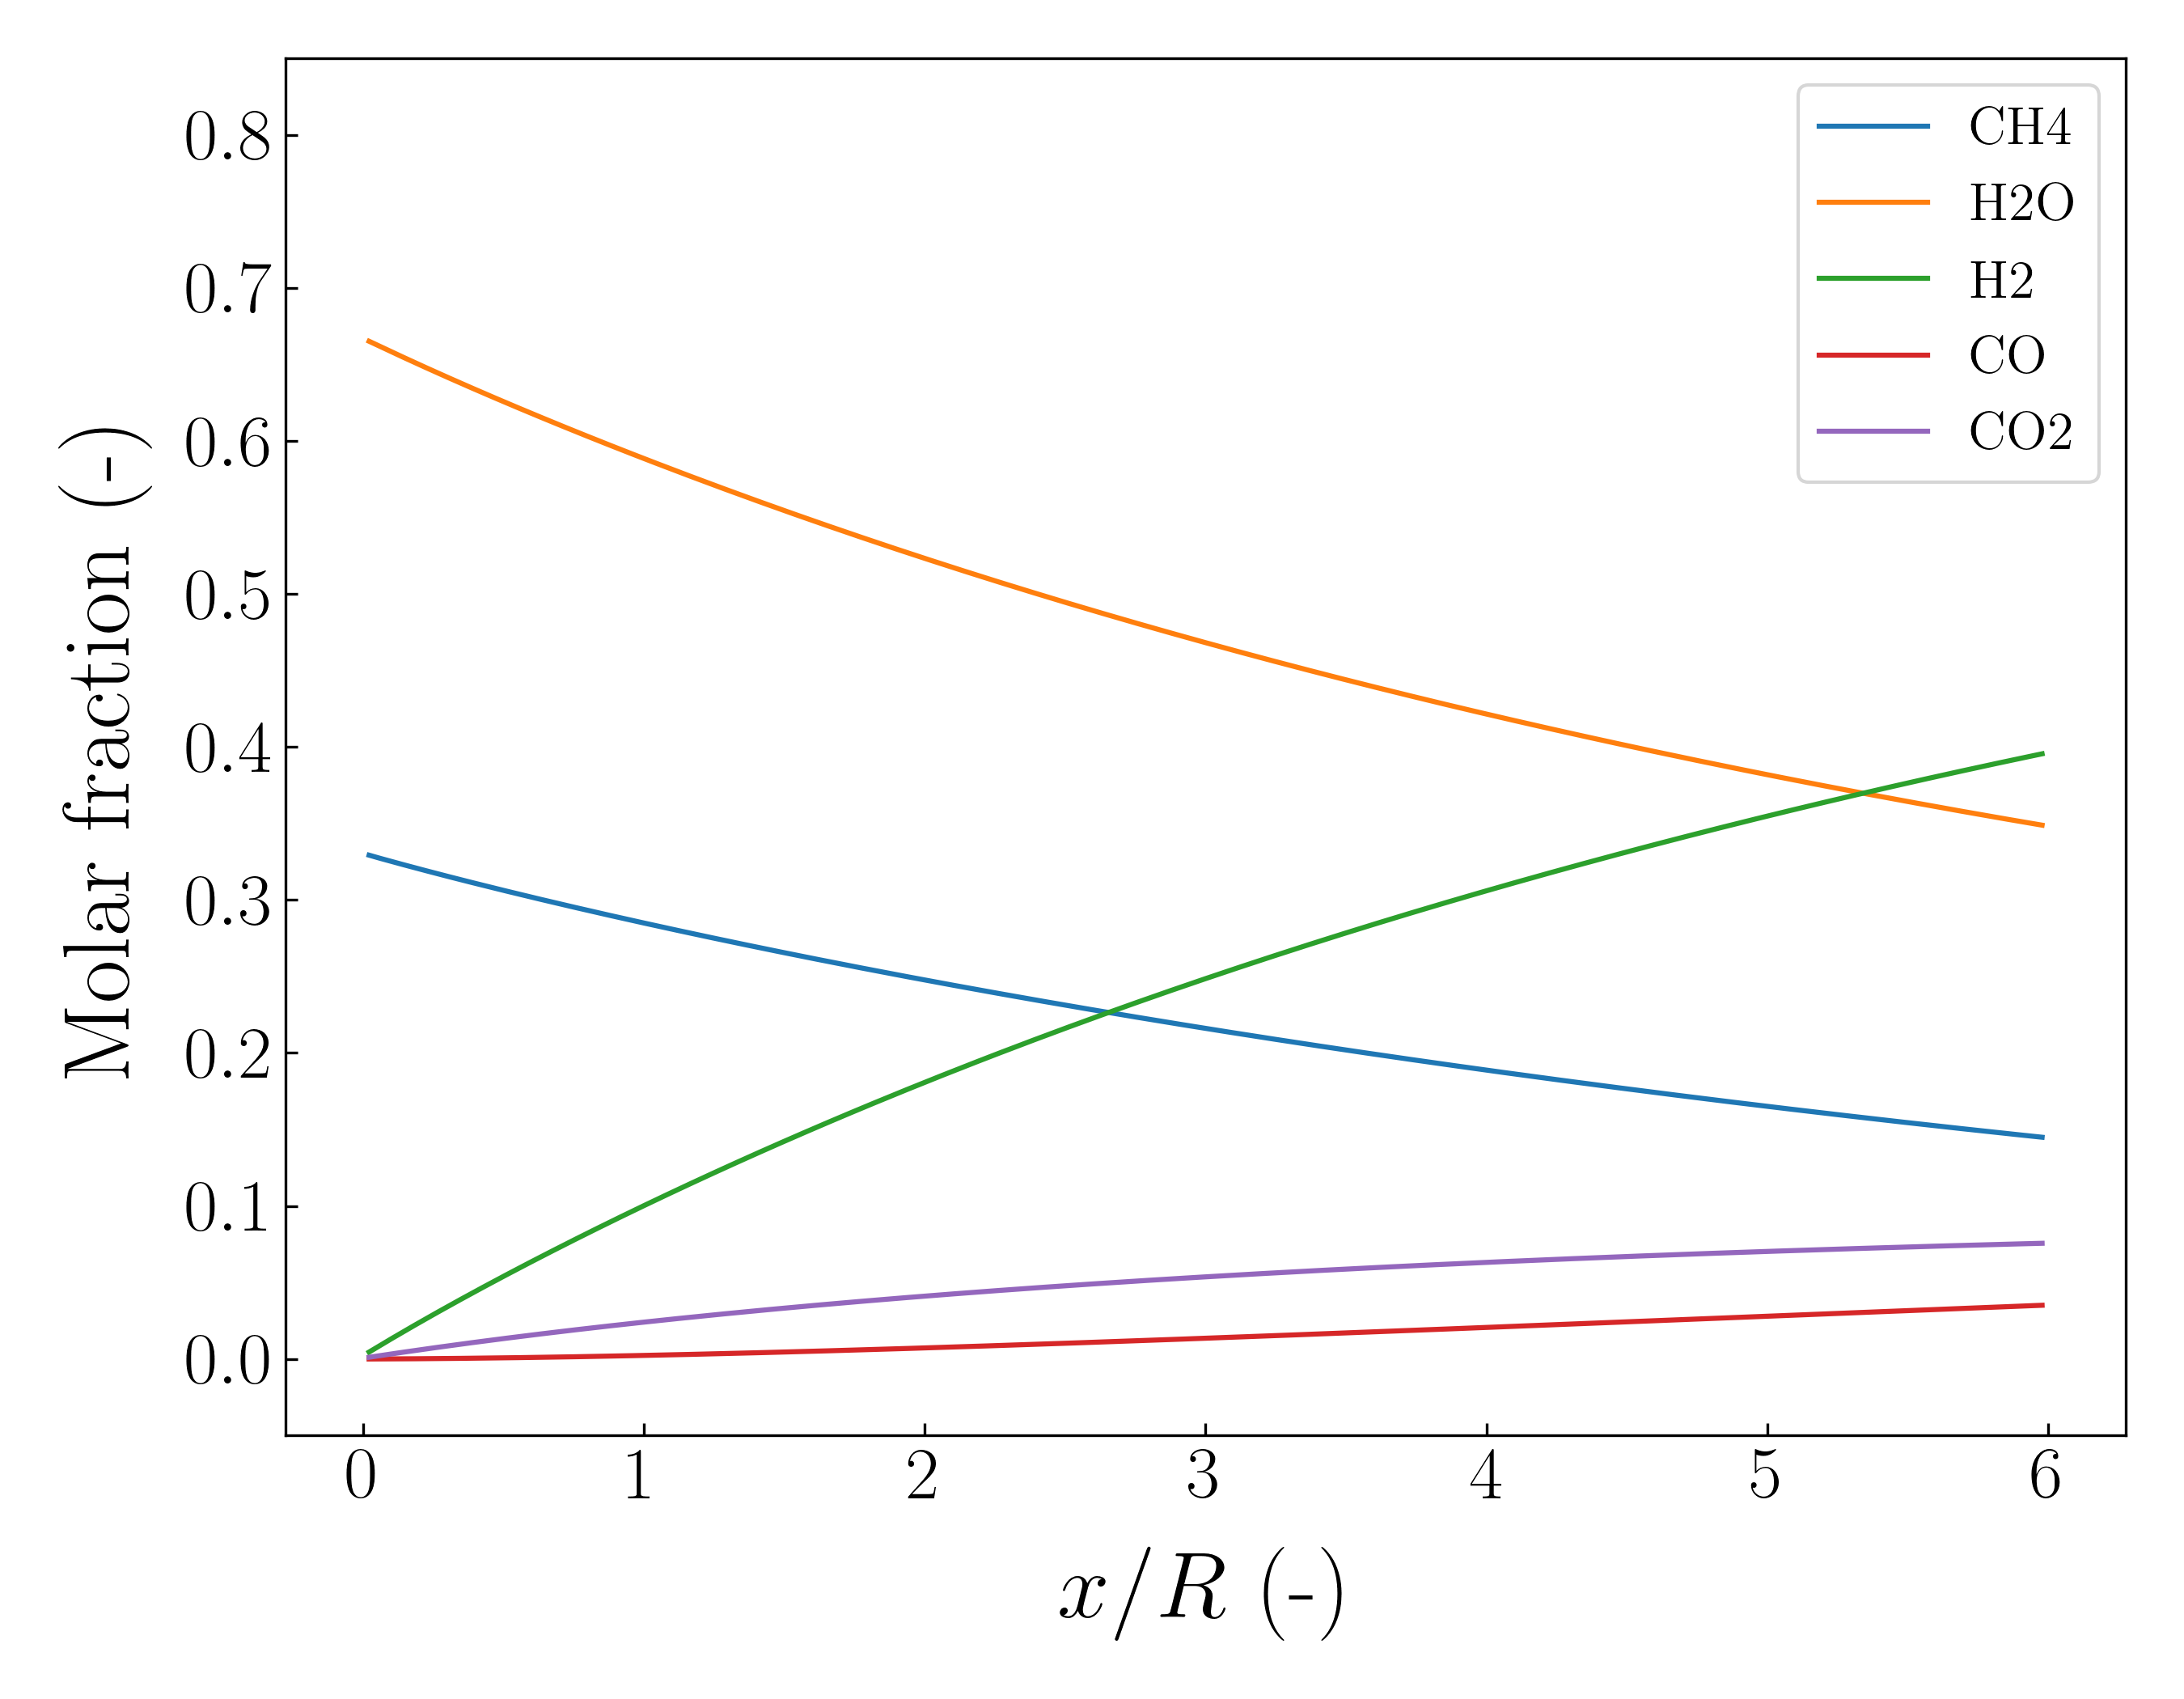
\includegraphics[width=80mm]{results/5/60C_40T/GEN30-AVG.png}
%\caption{\label{fig:5R6040G30-avg} Strategy I - Radius-averaged molar fractions -  30$^{\rm{th}}$ generation ($w_{\rm{CH_4}} = 0.6, w_T = 0.4$, $T_{\rm{in}}$ = 900 K, $u_{\rm{in}}$ = 0.15 m s$^{-1}$, $SC$ = 2.0)}
%\end{figure}
%
%\begin{figure}[h!]
%\centering
%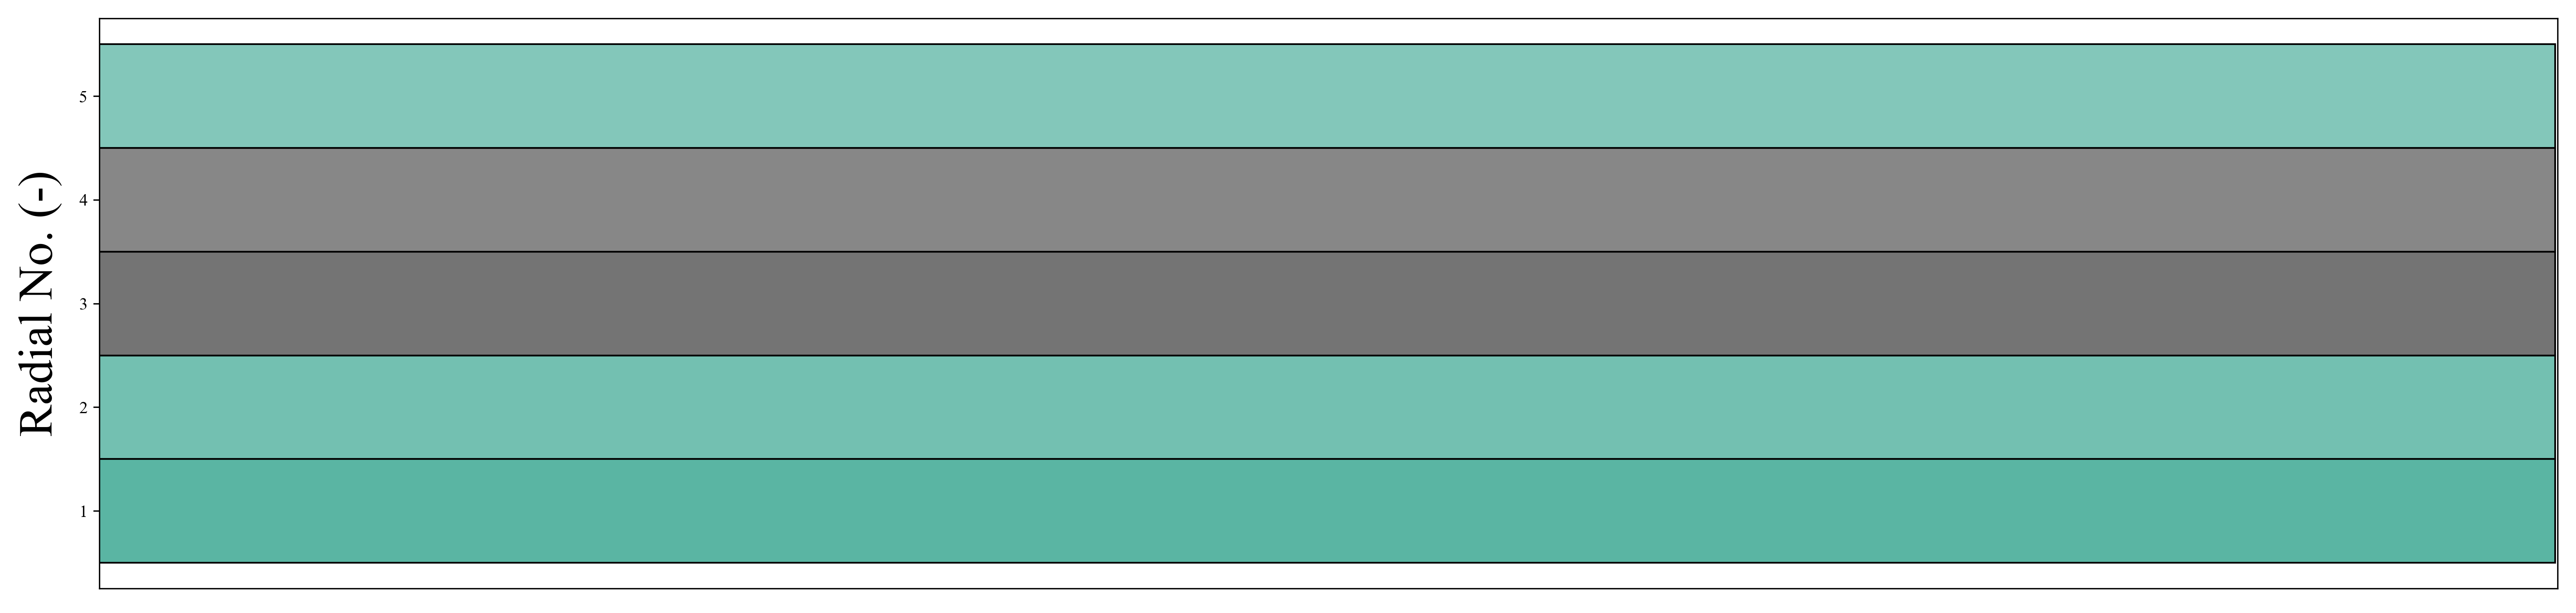
\includegraphics[width=120mm]{results/segments/5seg/60C40T/seg.png}
%\caption{\label{fig:30L6040G1-TField} Strategy I - Segments distribution for 30$^{\rm{th}}$ generation ($w_{\rm{CH_4}} = 0.6, w_T = 0.4$, $T_{\rm{in}}$ = 900 K, $u_{\rm{in}}$ = 0.15 m s$^{-1}$, $SC$ = 2.0)}
%\end{figure}
%
%\begin{figure}[h!]
%\centering
%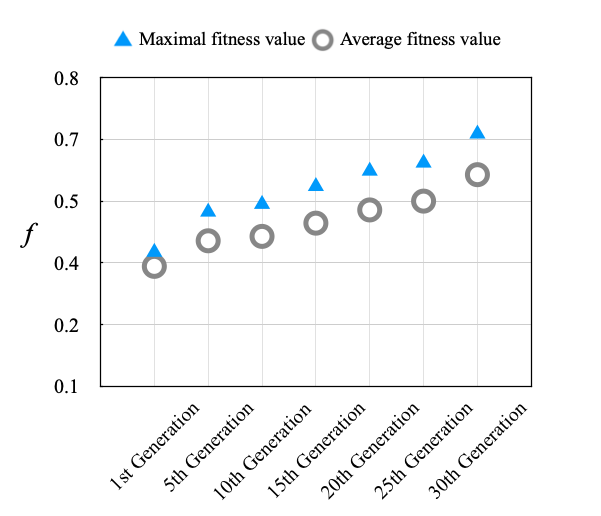
\includegraphics[width=100mm]{results/5/60C_40T.png}
%\caption{\label{fig:5R6040G-fitness} Strategy I - Fitness analysis throughout successive populations ($w_{\rm{CH_4}} = 0.6, w_T = 0.4$, $T_{\rm{in}}$ = 900 K, $u_{\rm{in}}$ = 0.15 m s$^{-1}$, $SC$ = 2.0)}
%\end{figure}
%
%\clearpage
%
%
%\paragraph{Thermal fitness 20 \%, methane conversion 80 \%} \hspace{0pt} \\
%\noindent 
%
%
%
%\begin{figure}[h!]
%\centering
%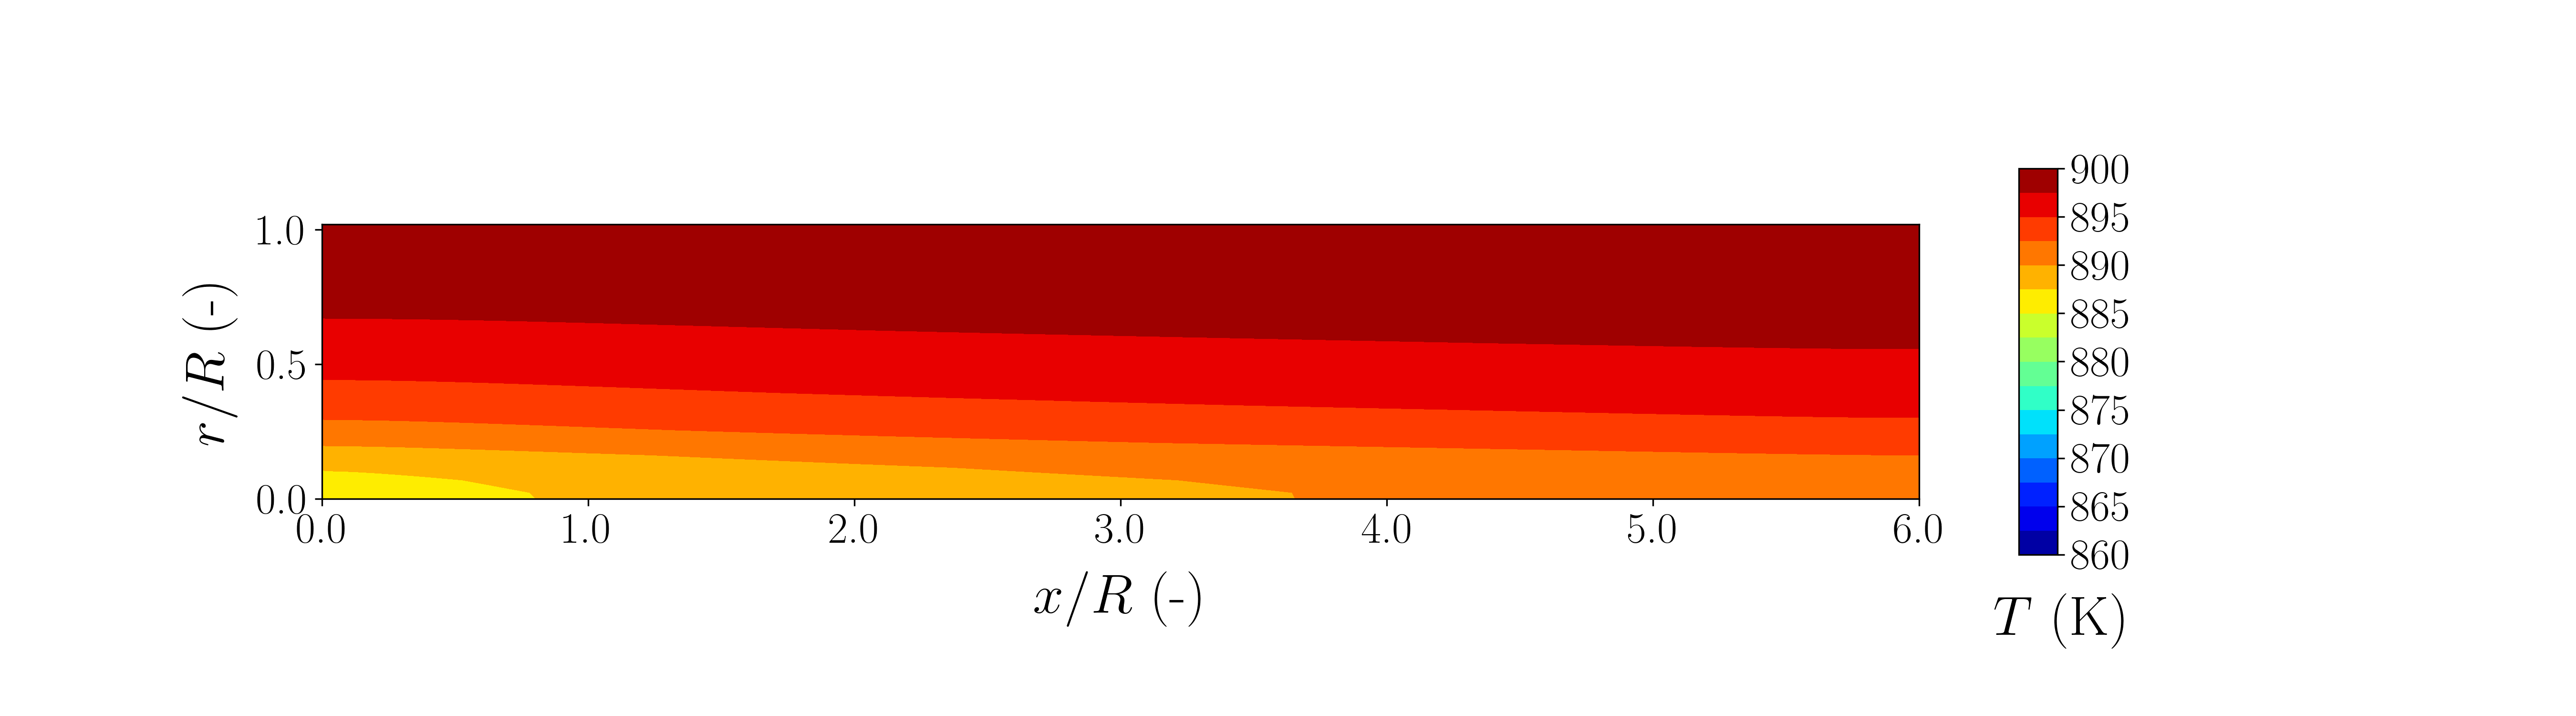
\includegraphics[width=190mm]{results/5/80C_20T/GEN1-TFIELD.png}
%\caption{\label{fig:5R8020G1-TField} Strategy I - Temperature field distribution - 1$^{\rm{st}}$ generation ($w_{\rm{CH_4}} = 0.8, w_T = 0.2$, $T_{\rm{in}}$ = 900 K, $u_{\rm{in}}$ = 0.15 m s$^{-1}$, $SC$ = 2.0)}
%\end{figure}
%
%\begin{figure}[h!]
%\centering
%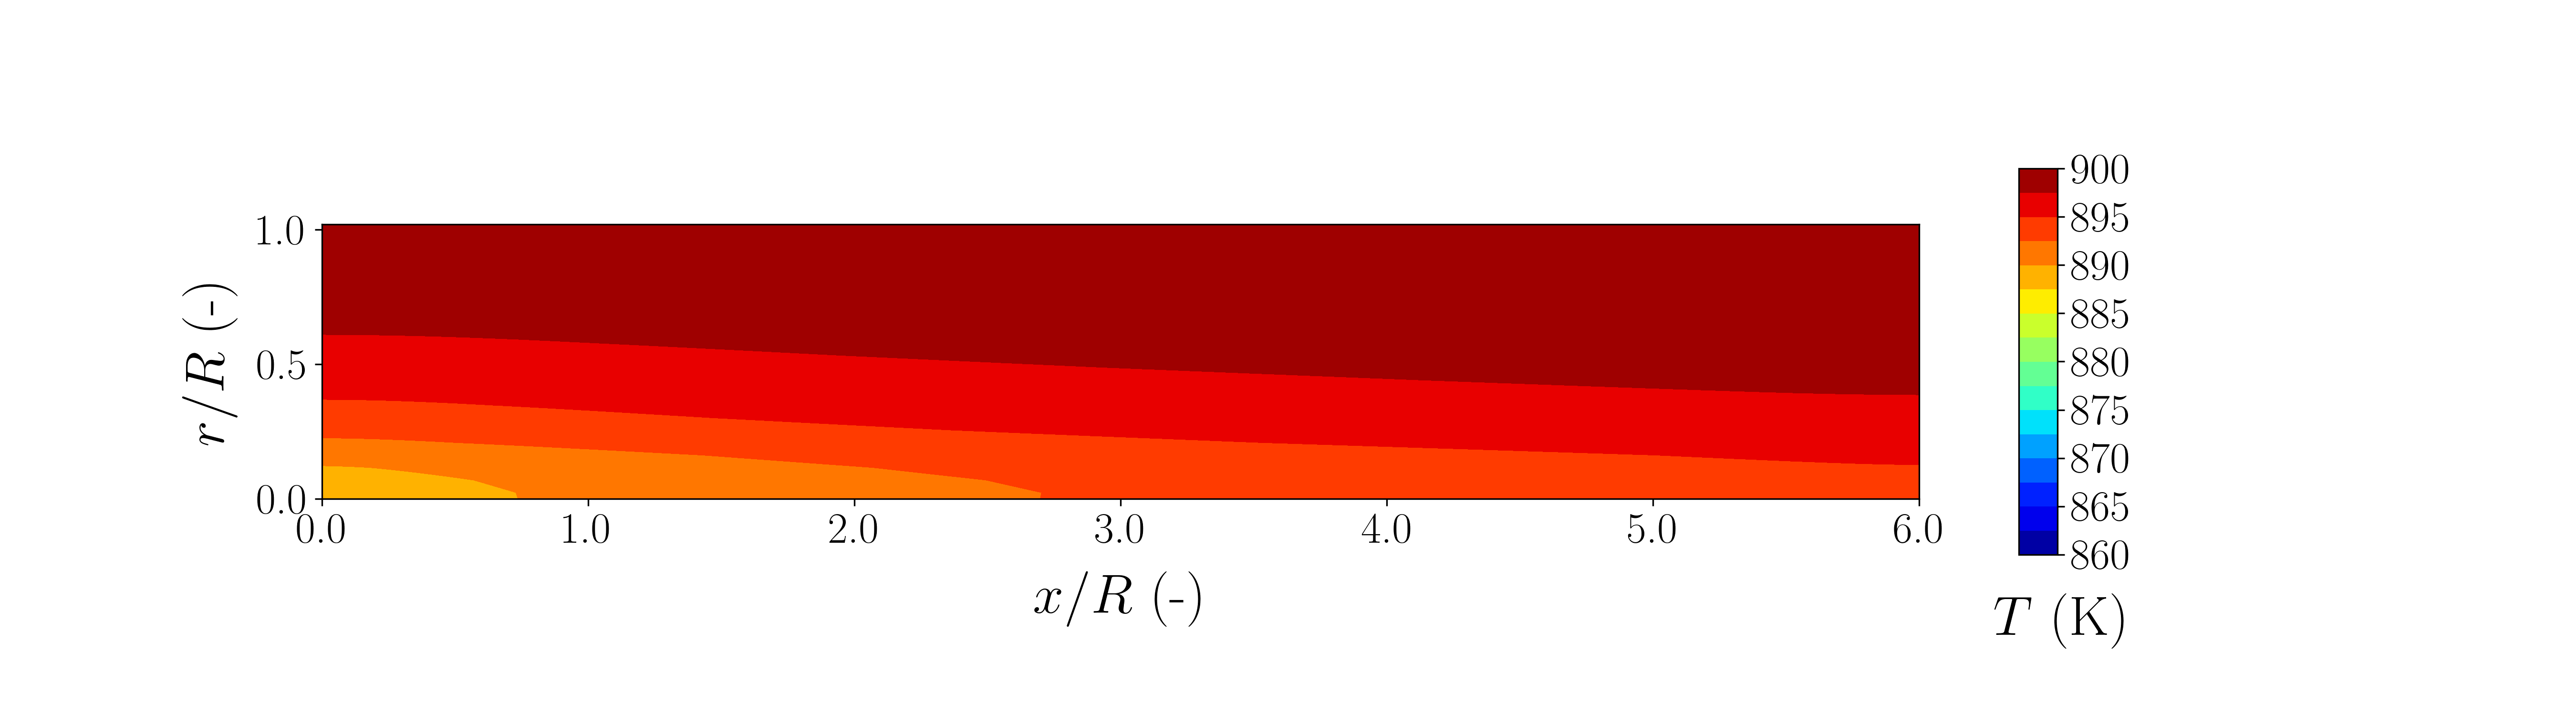
\includegraphics[width=190mm]{results/5/80C_20T/GEN15-TFIELD.png}
%\caption{\label{fig:5R8020G15-TField} Strategy I - Temperature field distribution - 15$^{\rm{th}}$ generation ($w_{\rm{CH_4}} = 0.8, w_T = 0.2$, $T_{\rm{in}}$ = 900 K, $u_{\rm{in}}$ = 0.15 m s$^{-1}$, $SC$ = 2.0)}
%\end{figure}
%
%\begin{figure}[h!]
%\centering
%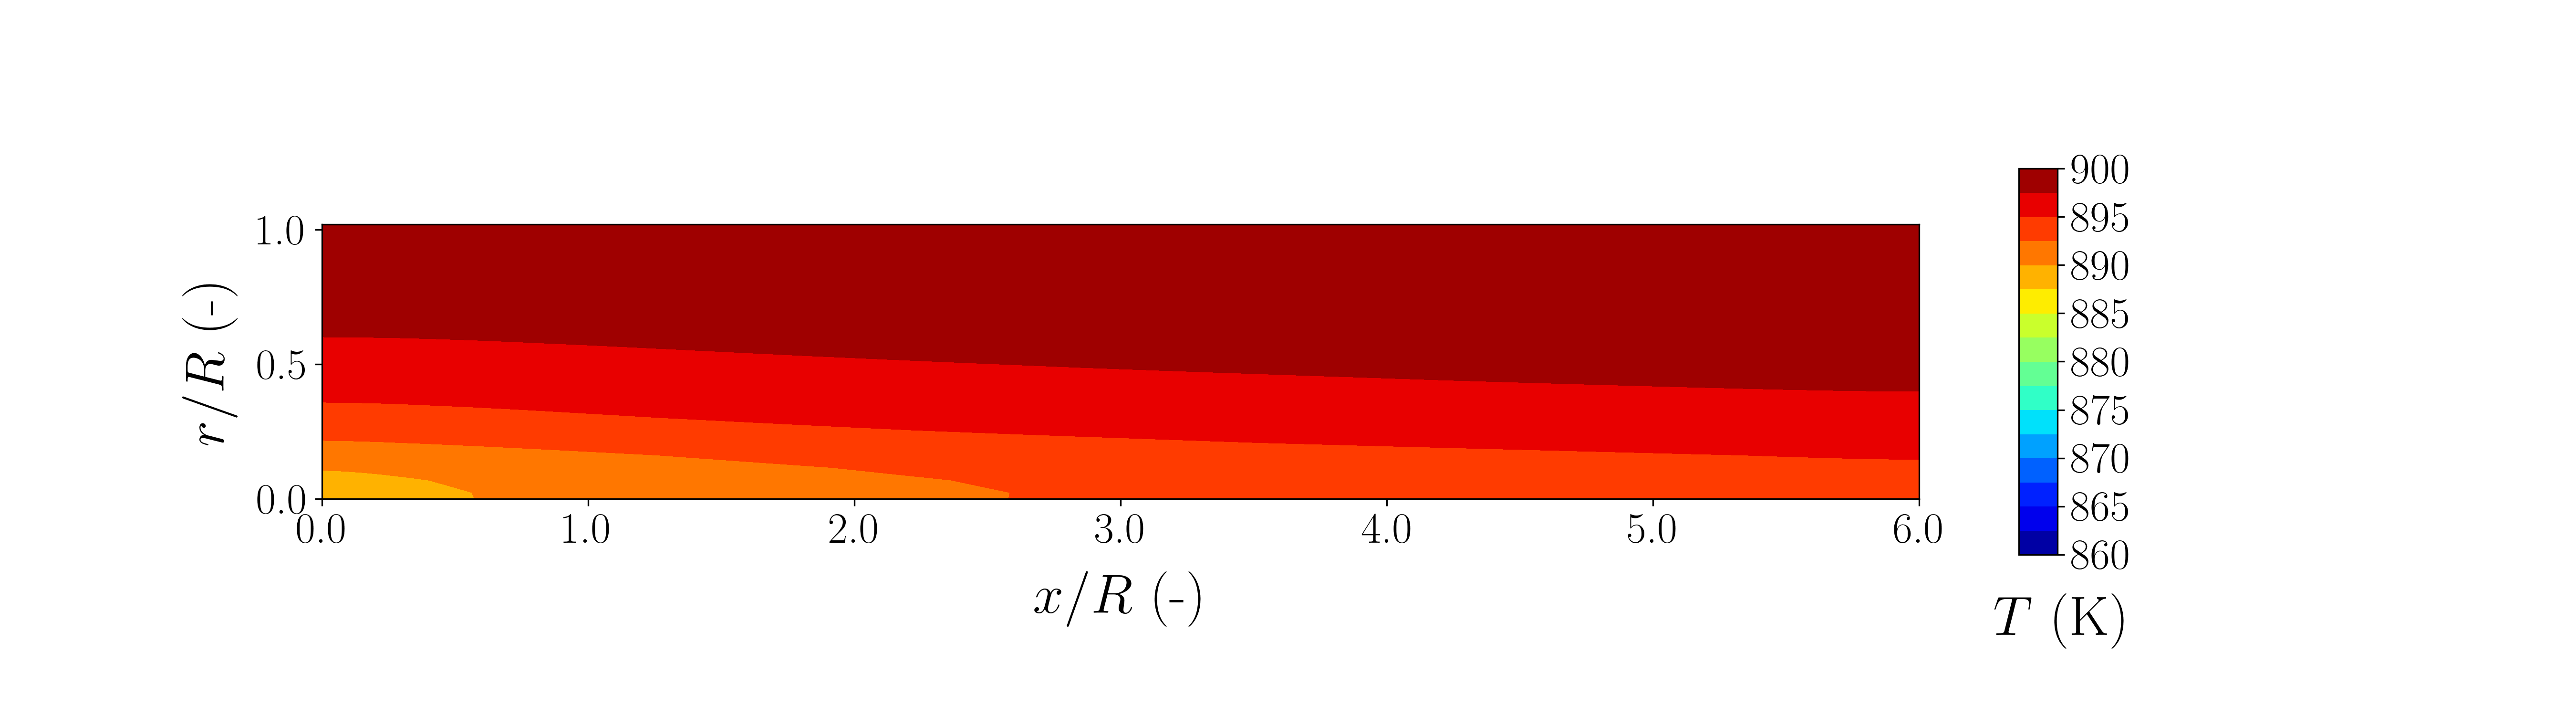
\includegraphics[width=190mm]{results/5/80C_20T/GEN30-TFIELD.png}
%\caption{\label{fig:5R8020G30-TField} Strategy I - Temperature field distribution - 30$^{\rm{th}}$ generation ($w_{\rm{CH_4}} = 0.8, w_T = 0.2$, $T_{\rm{in}}$ = 900 K, $u_{\rm{in}}$ = 0.15 m s$^{-1}$, $SC$ = 2.0)}
%\end{figure}
%
%
%\begin{figure}[h!]
%\centering
%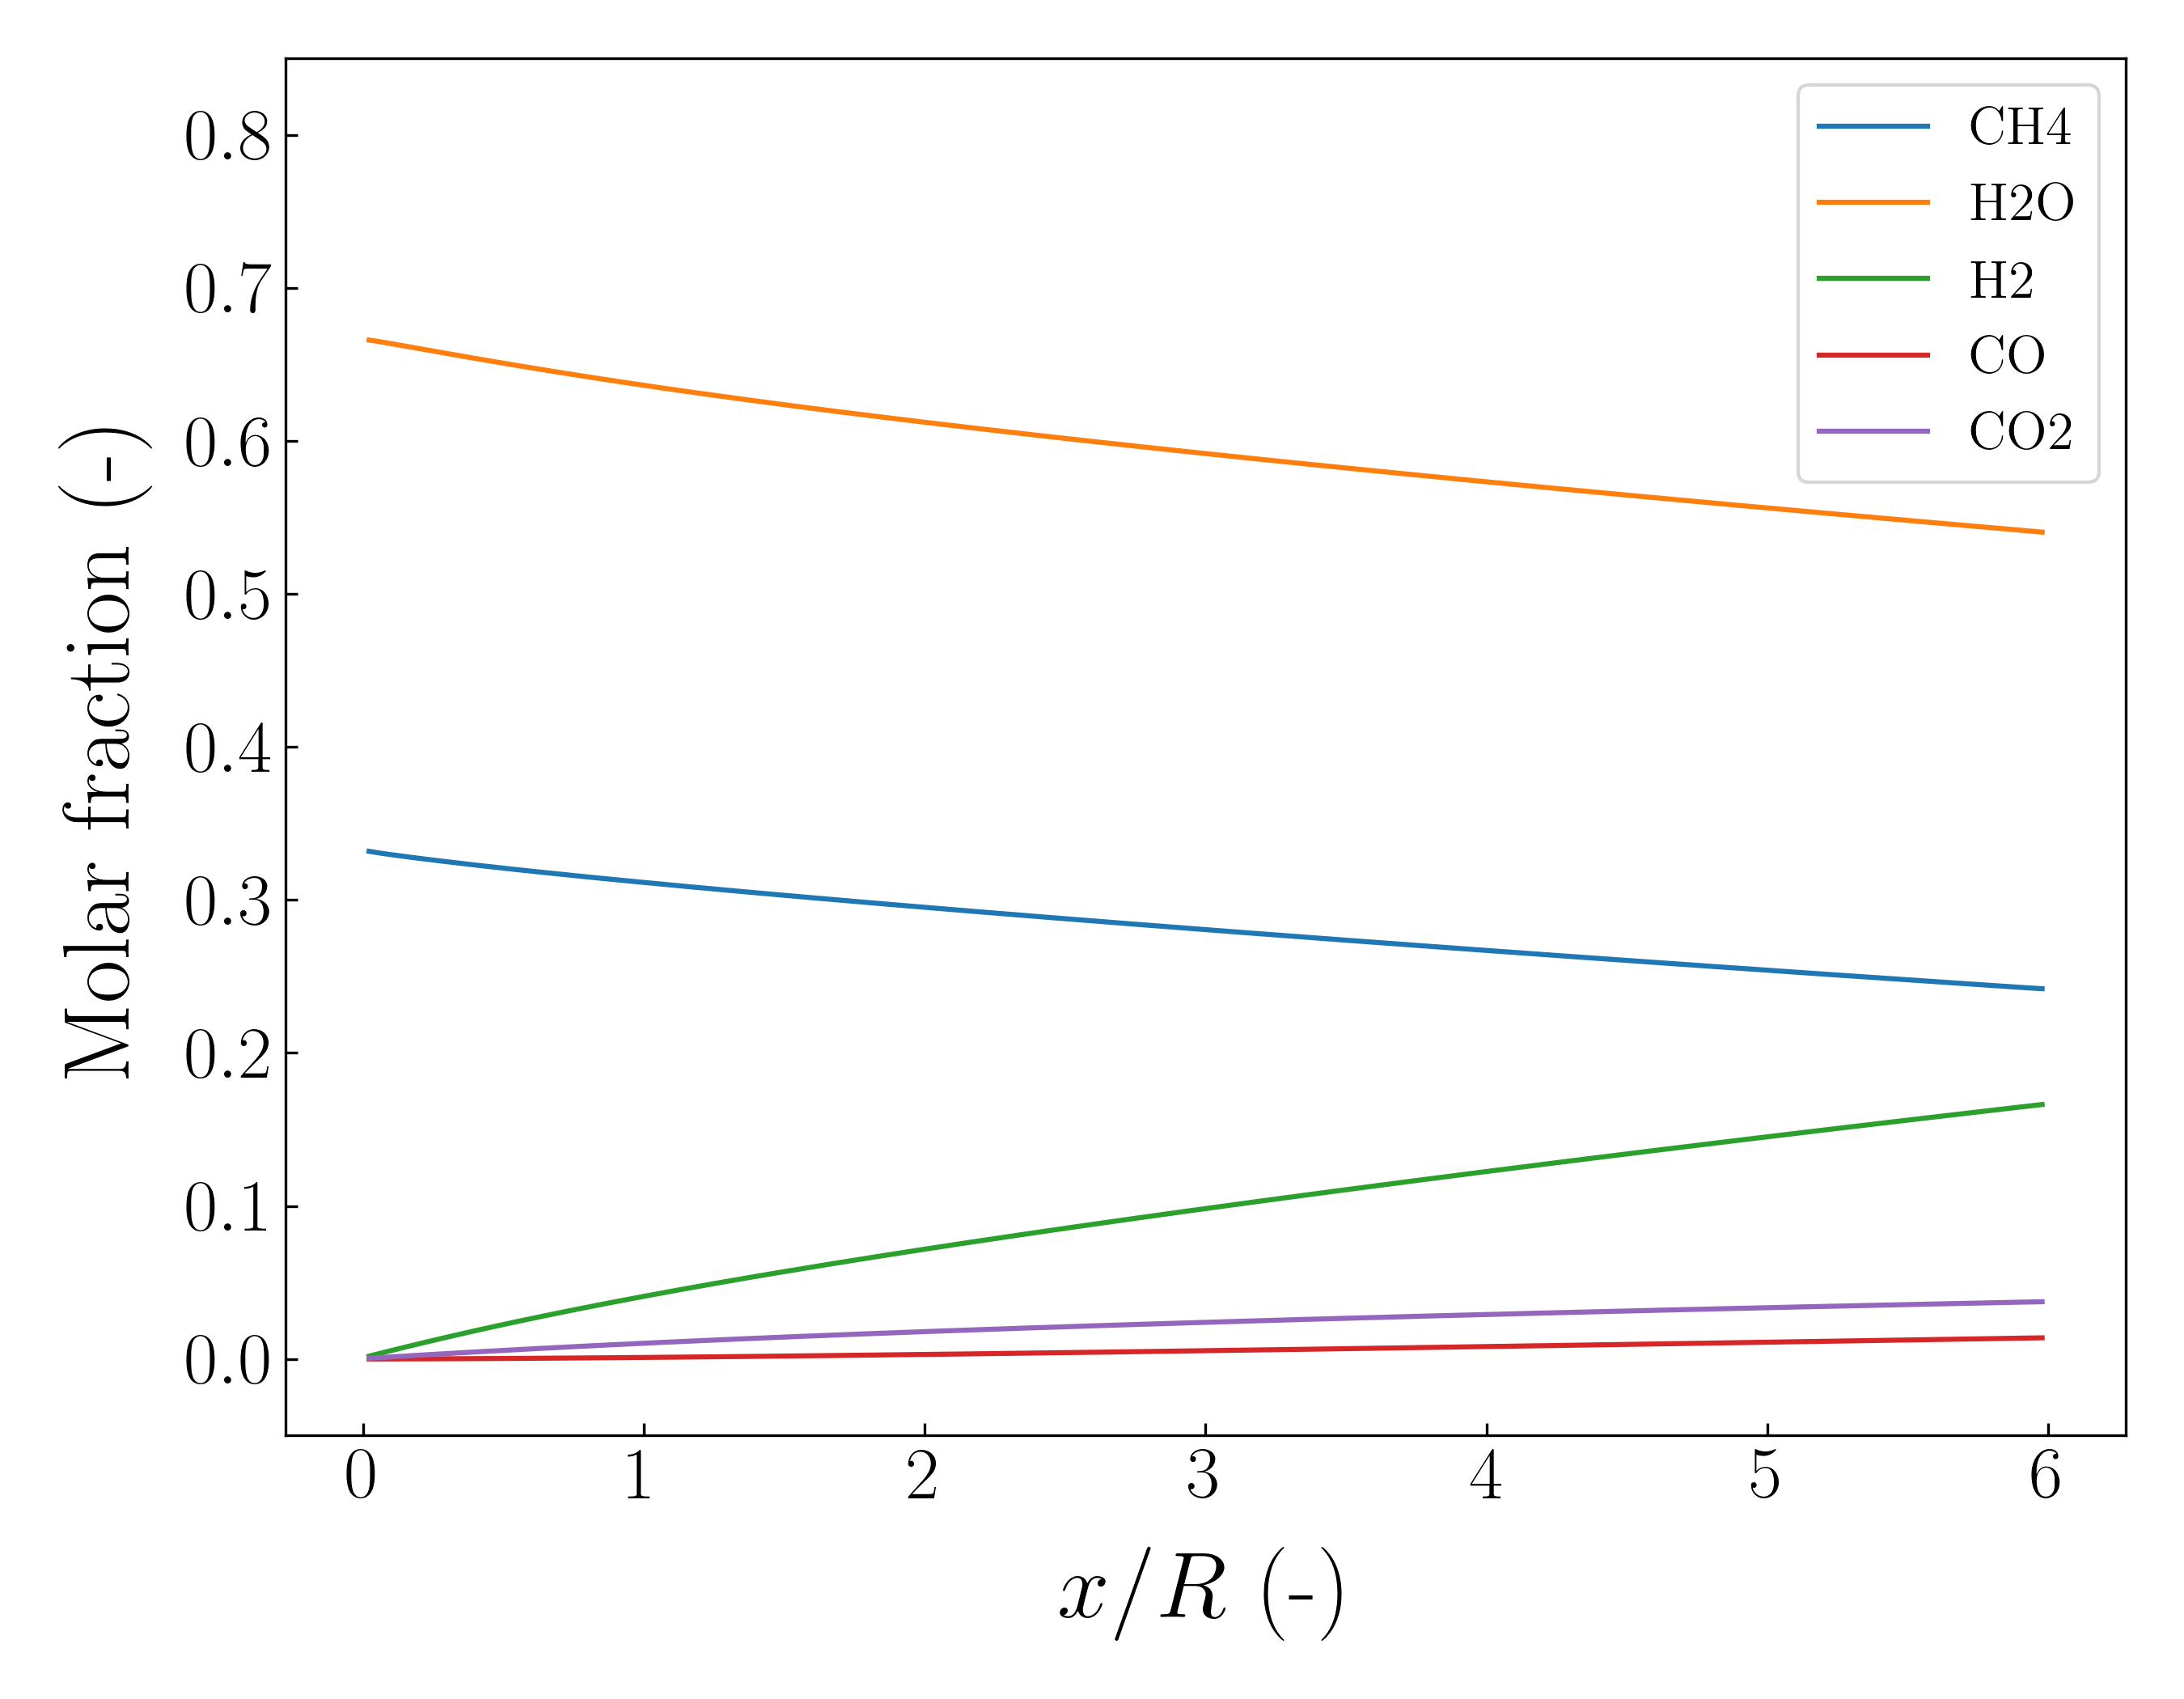
\includegraphics[width=80mm]{results/5/80C_20T/GEN1-AVG.png}
%\caption{\label{fig:5R8020G1-avg} Strategy I - Radius-averaged molar fractions - 1$^{\rm{st}}$ generation ($w_{\rm{CH_4}} = 0.8, w_T = 0.2$, $T_{\rm{in}}$ = 900 K, $u_{\rm{in}}$ = 0.15 m s$^{-1}$, $SC$ = 2.0)}
%\end{figure}
%
%\begin{figure}[h!]
%\centering
%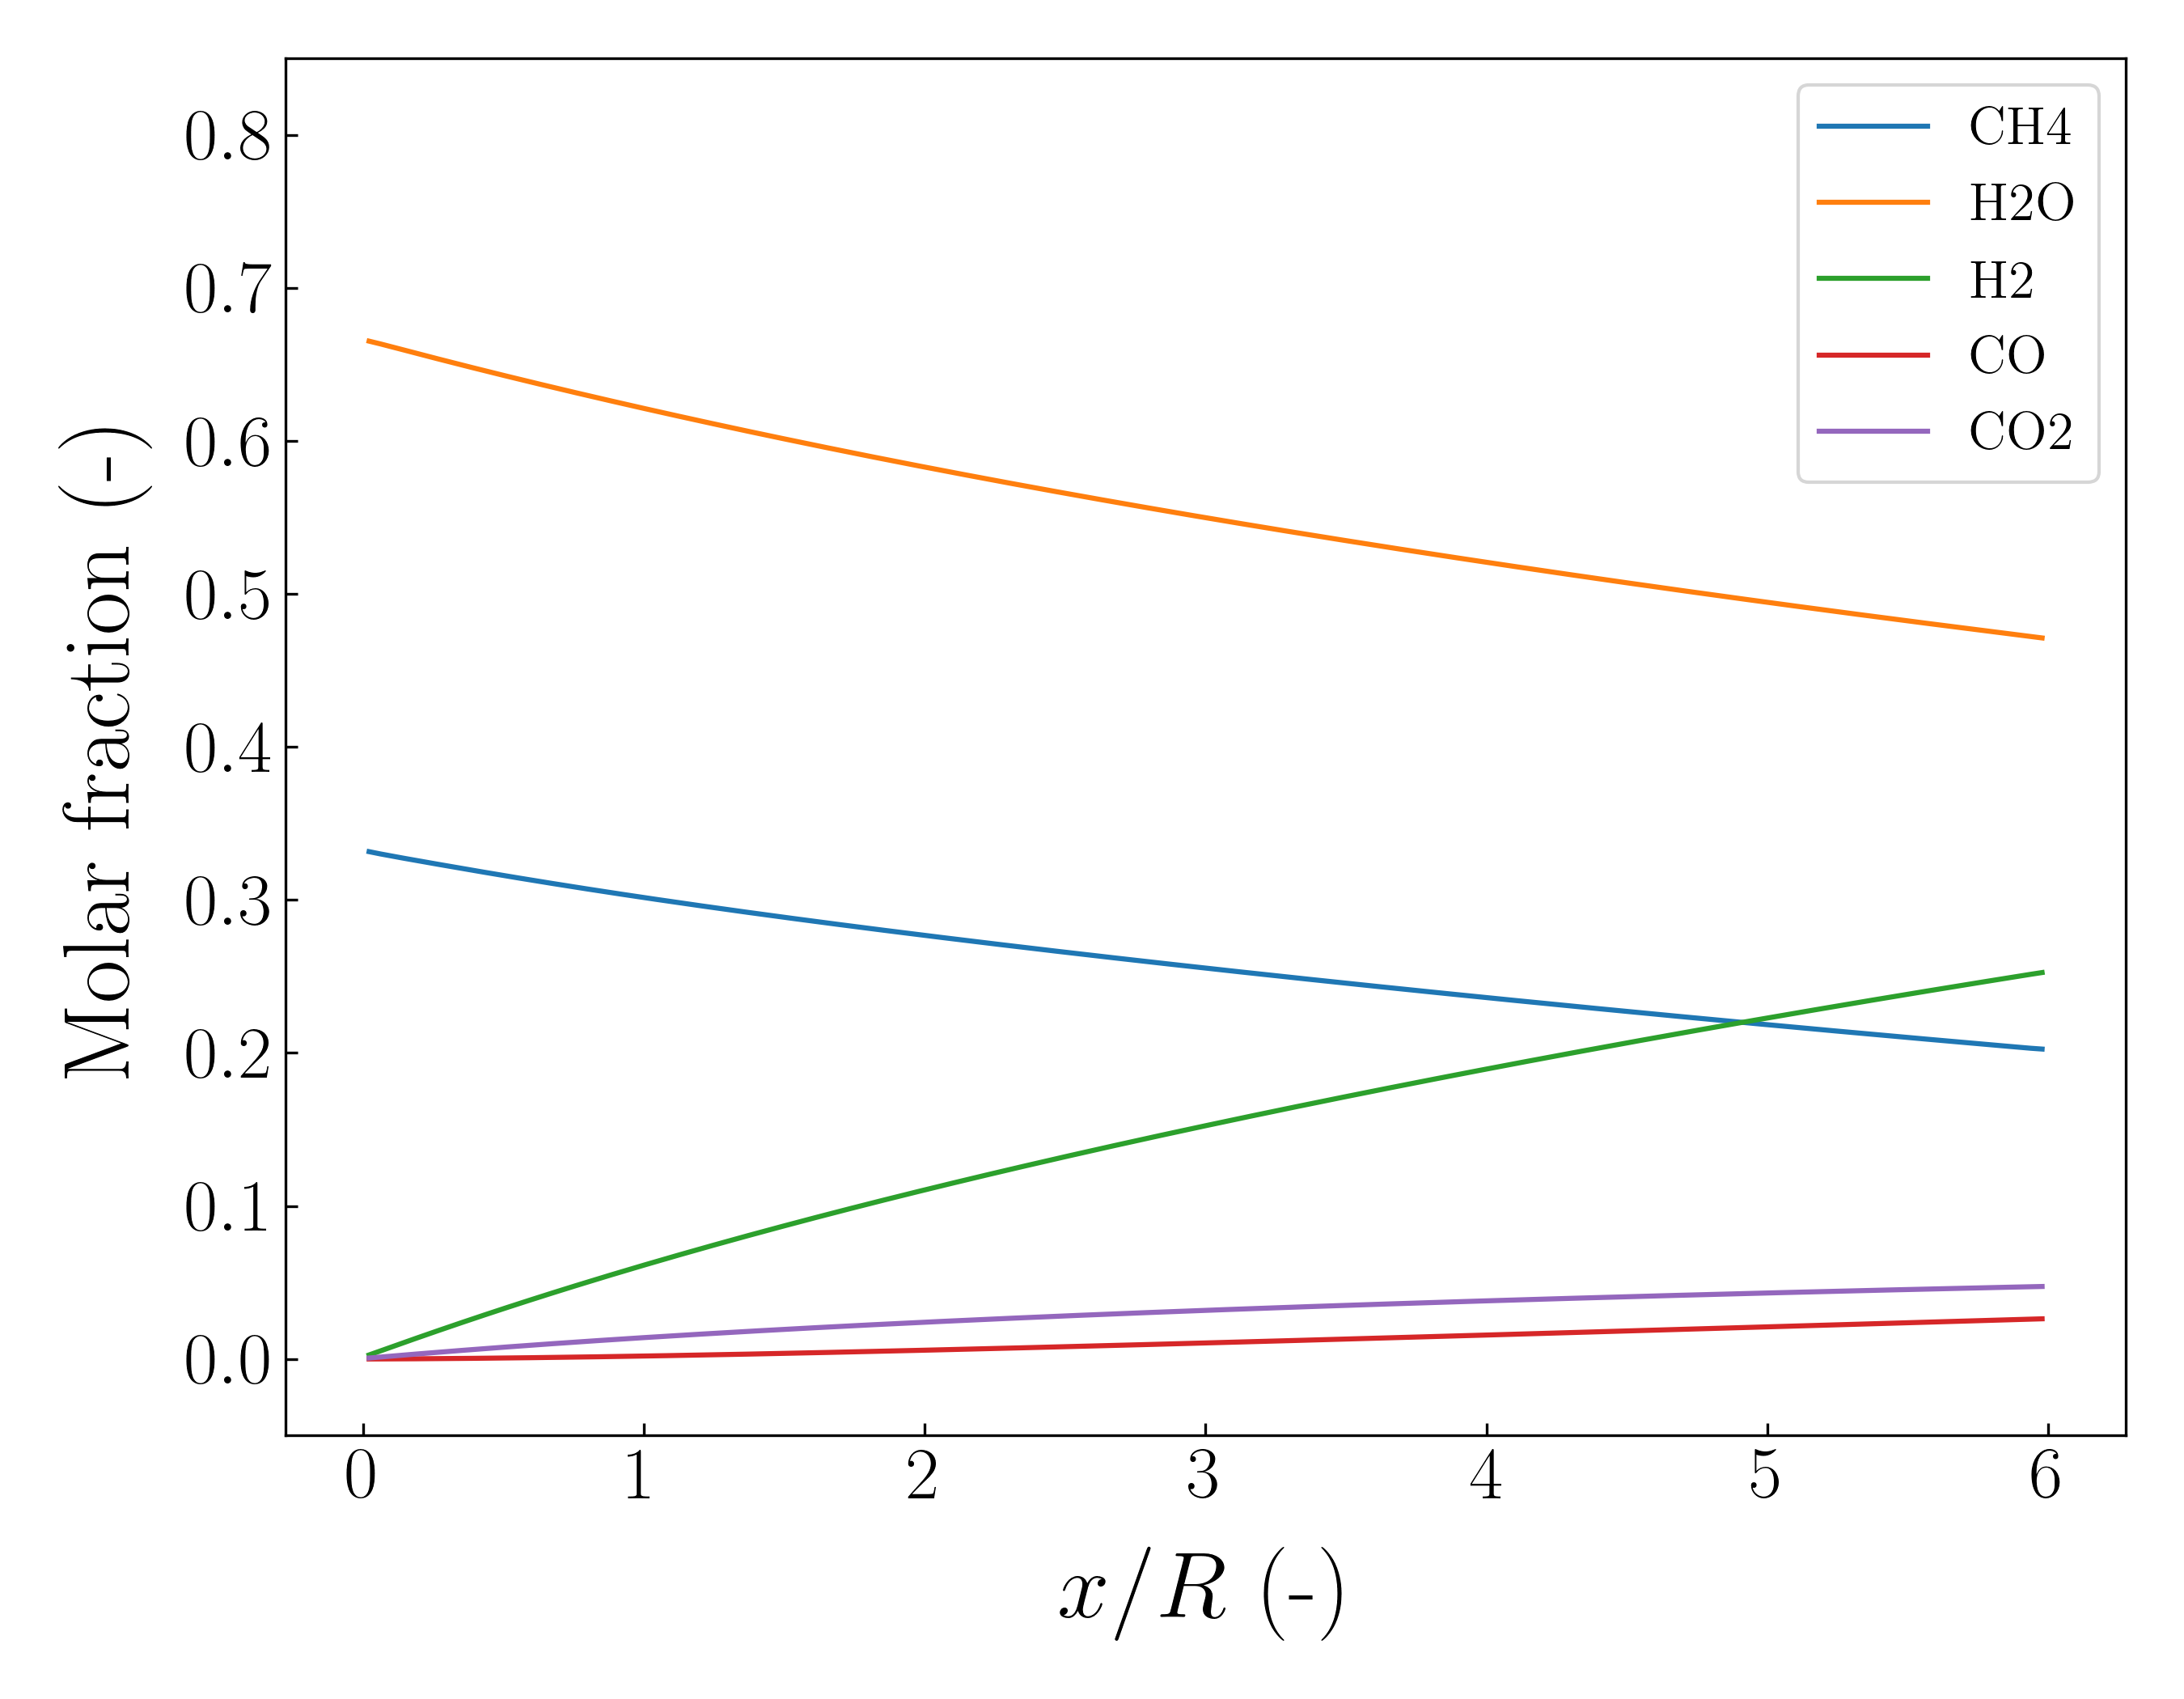
\includegraphics[width=80mm]{results/5/80C_20T/GEN15-AVG.png}
%\caption{\label{fig:5R8020G15-avg} Strategy I - Radius-averaged molar fractions - 15$^{\rm{th}}$ generation ($w_{\rm{CH_4}} = 0.8, w_T = 0.2$, $T_{\rm{in}}$ = 900 K, $u_{\rm{in}}$ = 0.15 m s$^{-1}$, $SC$ = 2.0)}
%\end{figure}
%
%\begin{figure}[h!]
%\centering
%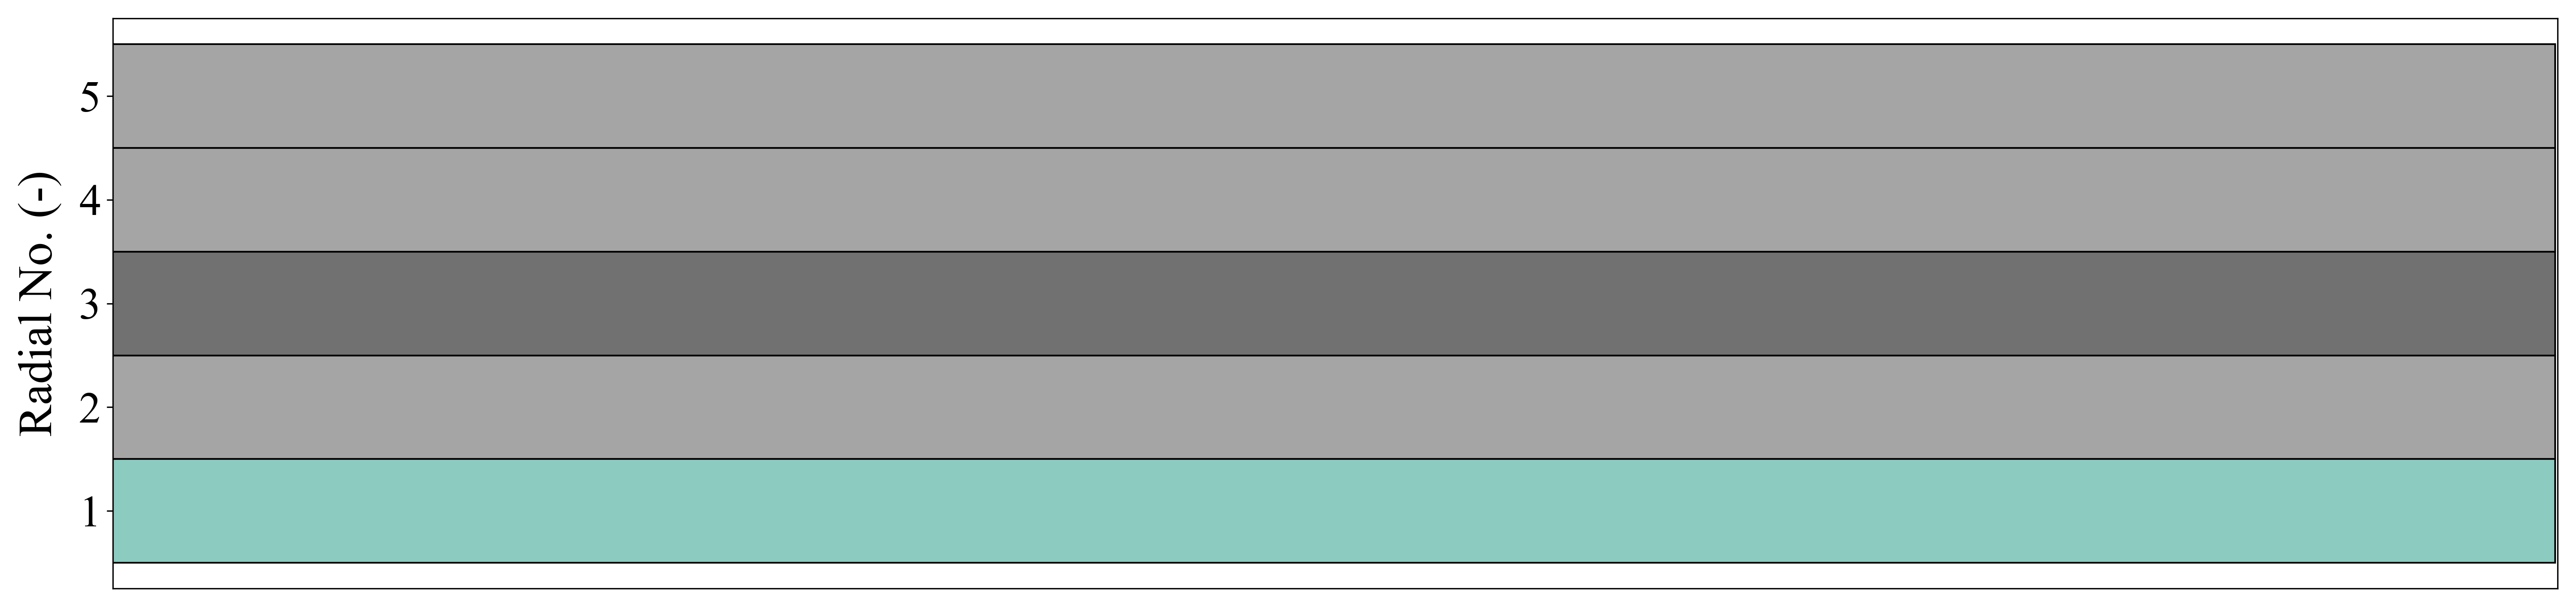
\includegraphics[width=120mm]{results/segments/5seg/80C20T/seg.png}
%\caption{\label{fig:30L6040G1-TField} Strategy I - Segments distribution for 30$^{\rm{th}}$ generation ($w_{\rm{CH_4}} = 0.8, w_T = 0.2$, $T_{\rm{in}}$ = 900 K, $u_{\rm{in}}$ = 0.15 m s$^{-1}$, $SC$ = 2.0)}
%\end{figure}
%
%\begin{figure}[h!]
%\centering
%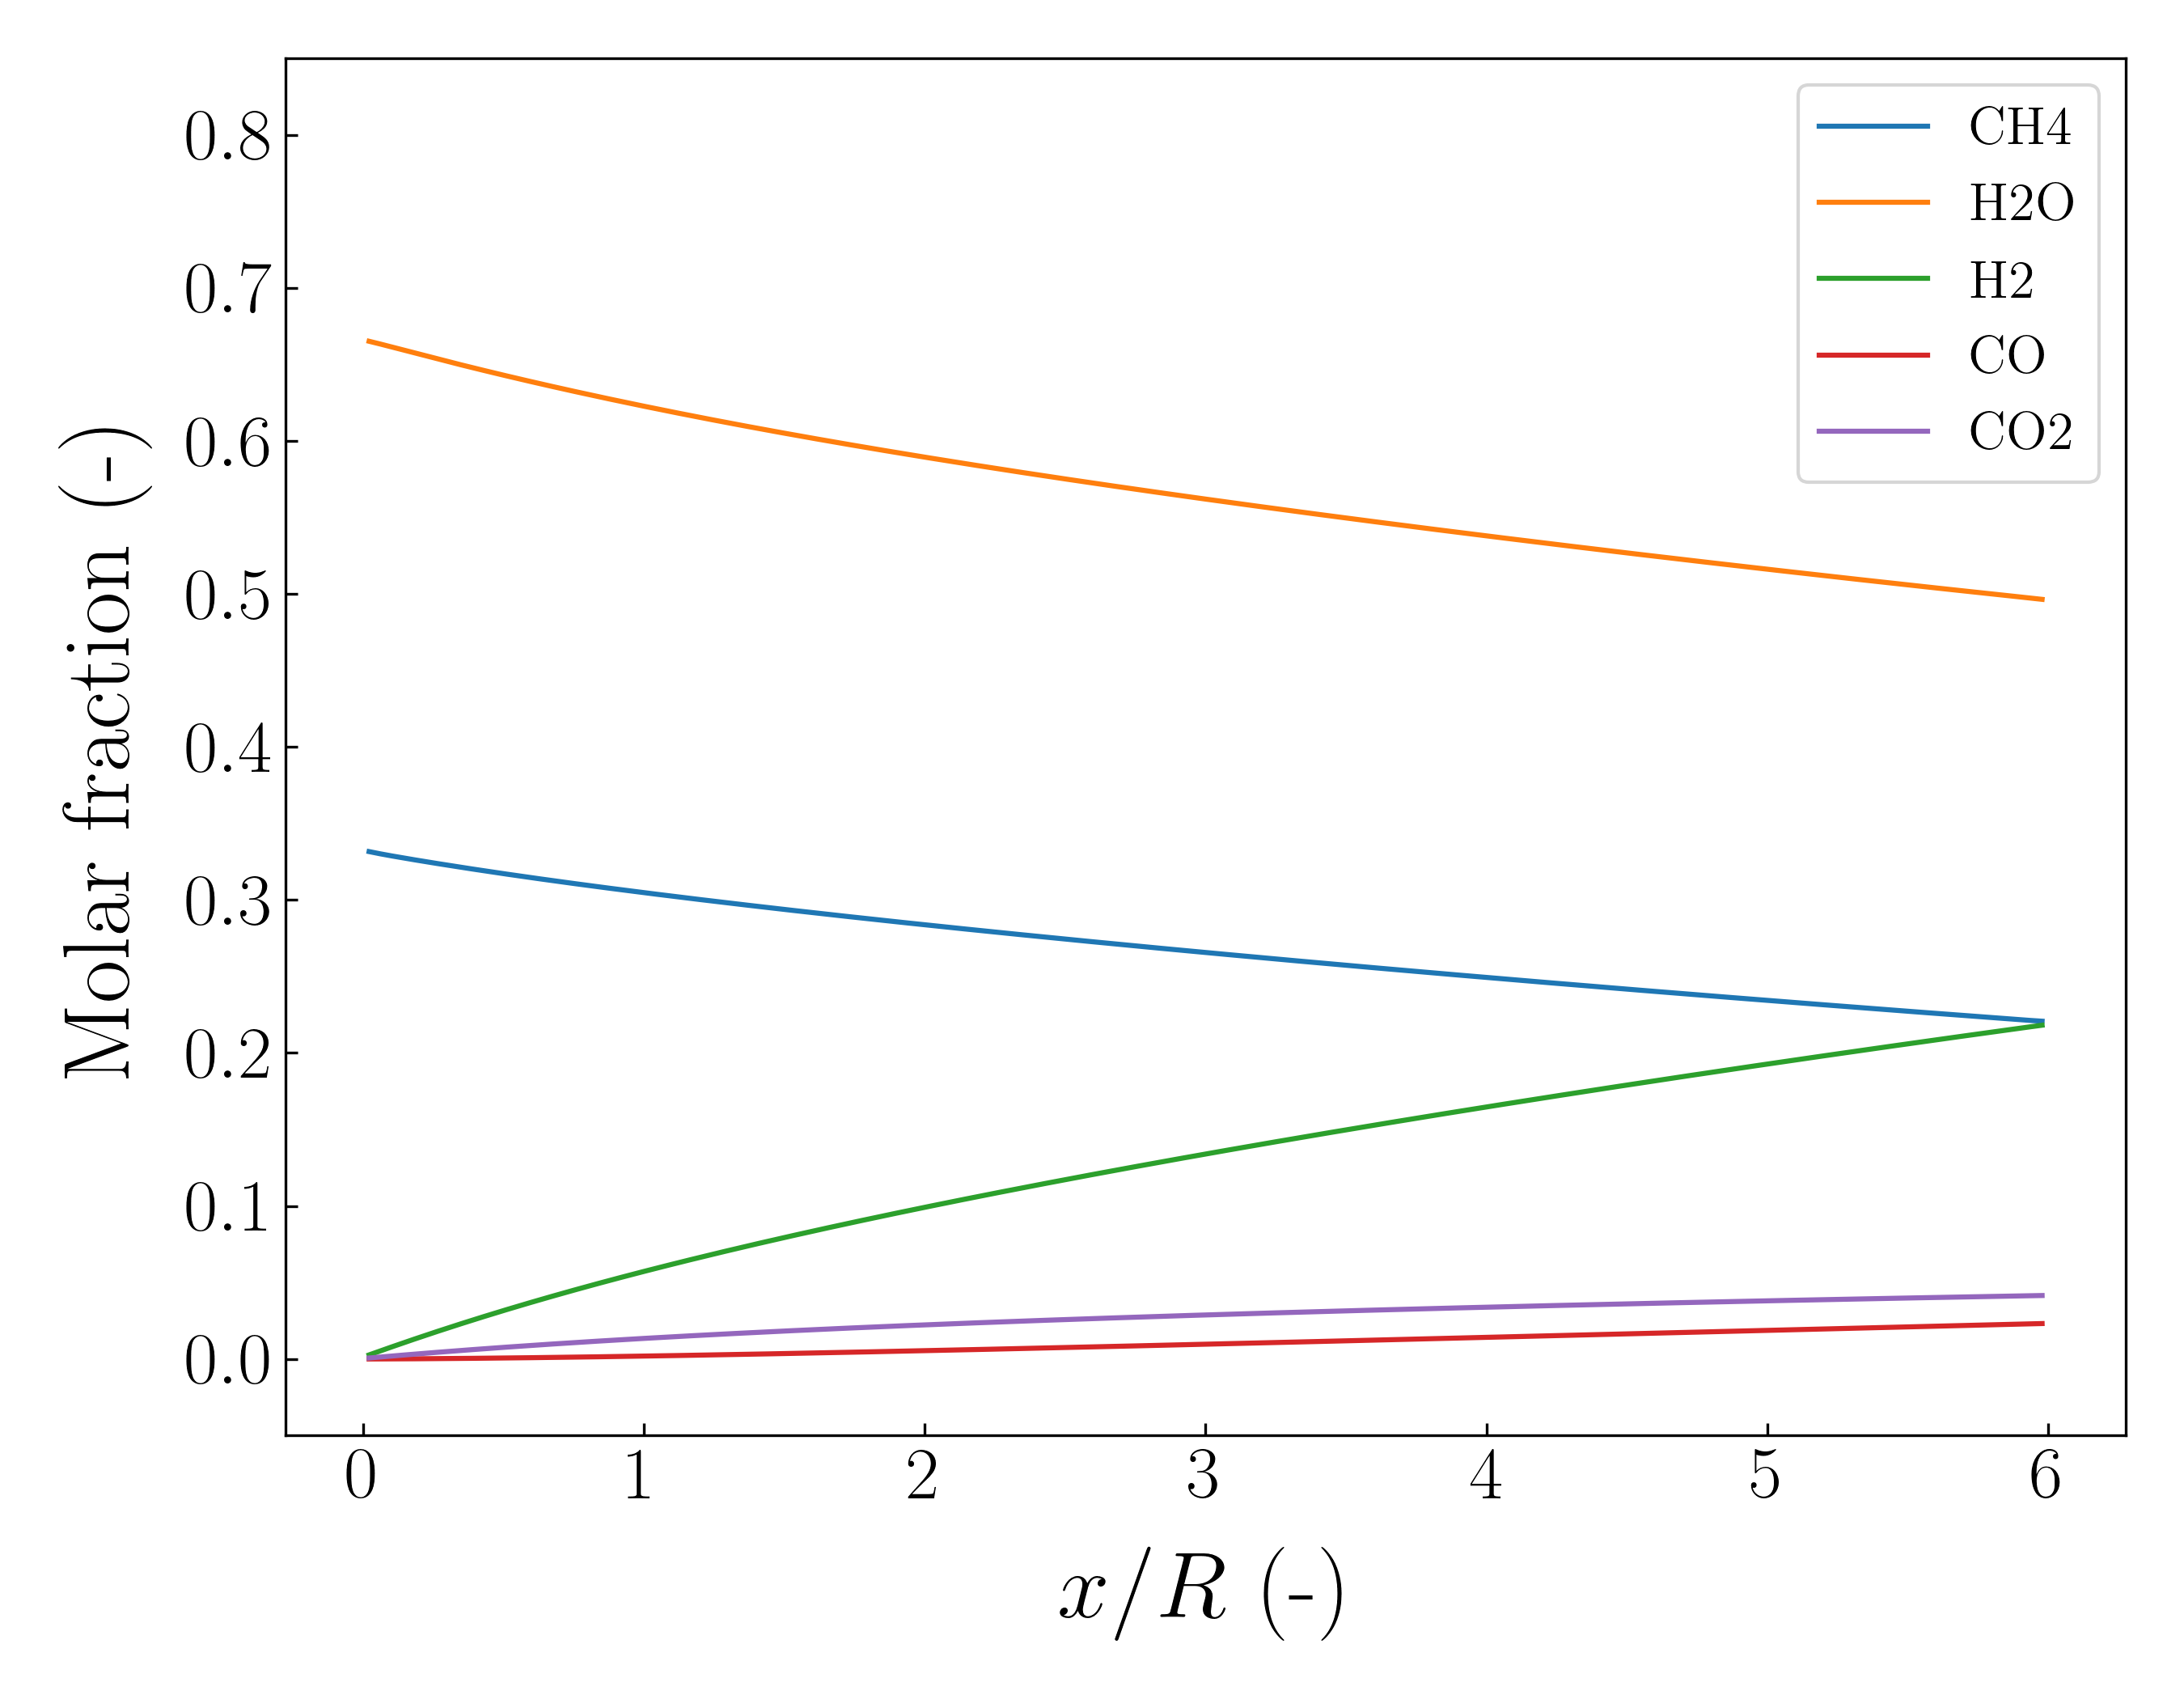
\includegraphics[width=80mm]{results/5/80C_20T/GEN30-AVG.png}
%\caption{\label{fig:5R8020G30-avg} Strategy I - Radius-averaged molar fractions -  30$^{\rm{th}}$ generation ($w_{\rm{CH_4}} = 0.8, w_T = 0.2$, $T_{\rm{in}}$ = 900 K, $u_{\rm{in}}$ = 0.15 m s$^{-1}$, $SC$ = 2.0)}
%\end{figure}
%
%
%The development of the fitness values among successive populations for strategy I is presented in Fig. \ref{fig:5R8020G-fitness}. 
%
%\begin{figure}
%\centering
%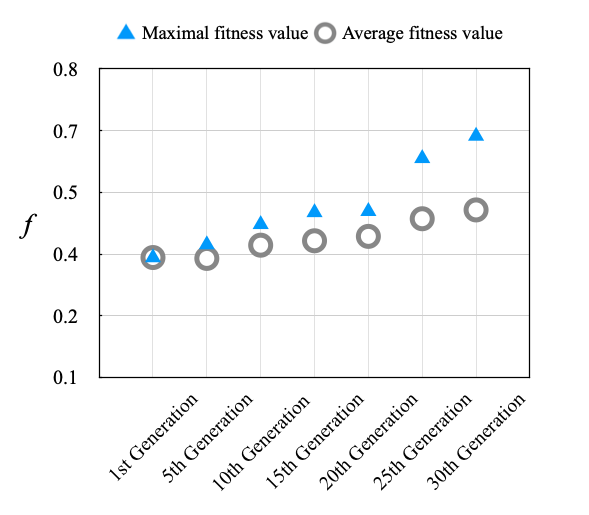
\includegraphics[width=100mm]{results/5/80C_20T.png}
%\caption{\label{fig:5R8020G-fitness} Strategy I - Fitness analysis throughout successive populations ($w_{\rm{CH_4}} = 0.8, w_T = 0.2$, $T_{\rm{in}}$ = 900 K, $u_{\rm{in}}$ = 0.15 m s$^{-1}$, $SC$ = 2.0)}
%\end{figure}
%
%To allow a straightforward comparison between the catalyst inserts division strategies, hydrogen productivity $\zeta$ is calculated for the optimal cases found by each algorithm. The hydrogen productivity is summarized in Table \ref{tab:5RH2prod}. 
%
%\begin{center}
%\begin{table}
%\centering
%\caption{Hydrogen productivity for the catalytic insert division strategy I}
%\label{tab:5RH2prod}
%\begin{tabular}{l|c|c|c}
%\hline\noalign{\smallskip}
% $w_{\rm{CH_4}}$ / $ w_T $ & $\rm{H_{2_{out}}}$ & $\iota$ & $\zeta$ \\
%\noalign{\smallskip}\hline\noalign{\smallskip}
%REF         & 0.581     & 1.00  &  0.581\\
%0.2 / 0.8   & 0.255     & 0.20  & 1.278 \\
%0.4 / 0.6   & 0.268     & 0.19  & 1.398 \\
%0.5 / 0.5   & 0.231     & 0.20  & 1.157 \\
%0.6 / 0.4   & 0.407     & 0.45  & 0.900 \\
%0.8 / 0.2   & 0.218     & 0.20  & 1.090 \\
%\noalign{\smallskip}\hline
%\end{tabular}
%\end{table}
%\end{center}
%
%
%\clearpage
%
%
%\subsection{Insert division strategy II}
%\label{subsec:5RE}
%
%\begin{figure}[h!]
%\centering
%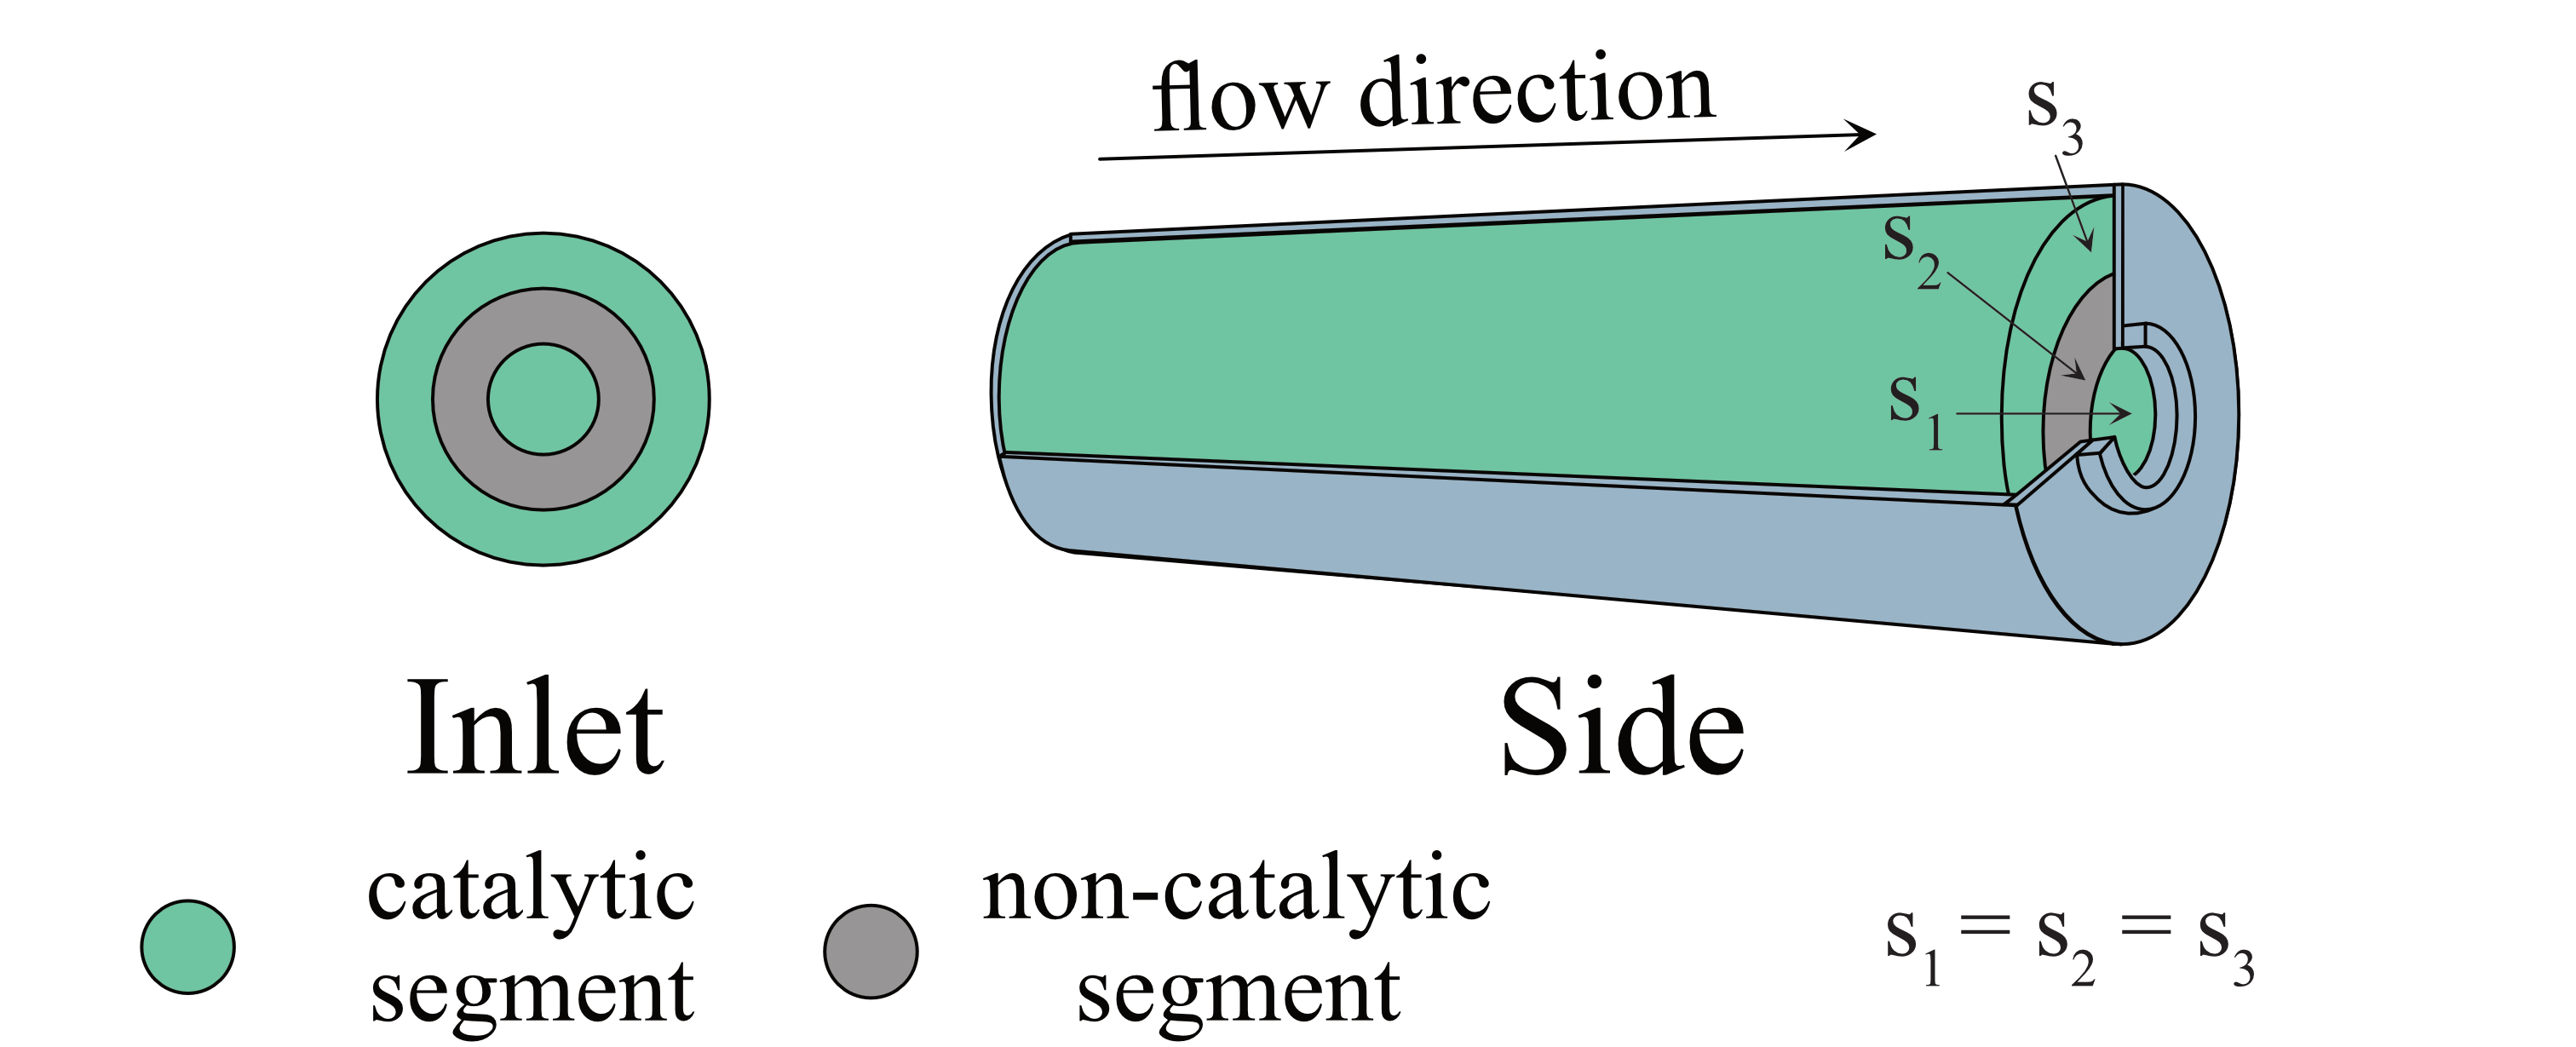
\includegraphics[width=120mm]{5segEqSurf.png}
%\caption{\label{fig:5segEqSurf}Catalytic insert division strategy II}
%\end{figure}
%
%
%\paragraph{Thermal fitness 80 \%, methane conversion 20 \%} \hspace{0pt} \\
%\noindent 
%
%
%\begin{figure}[h!]
%\centering
%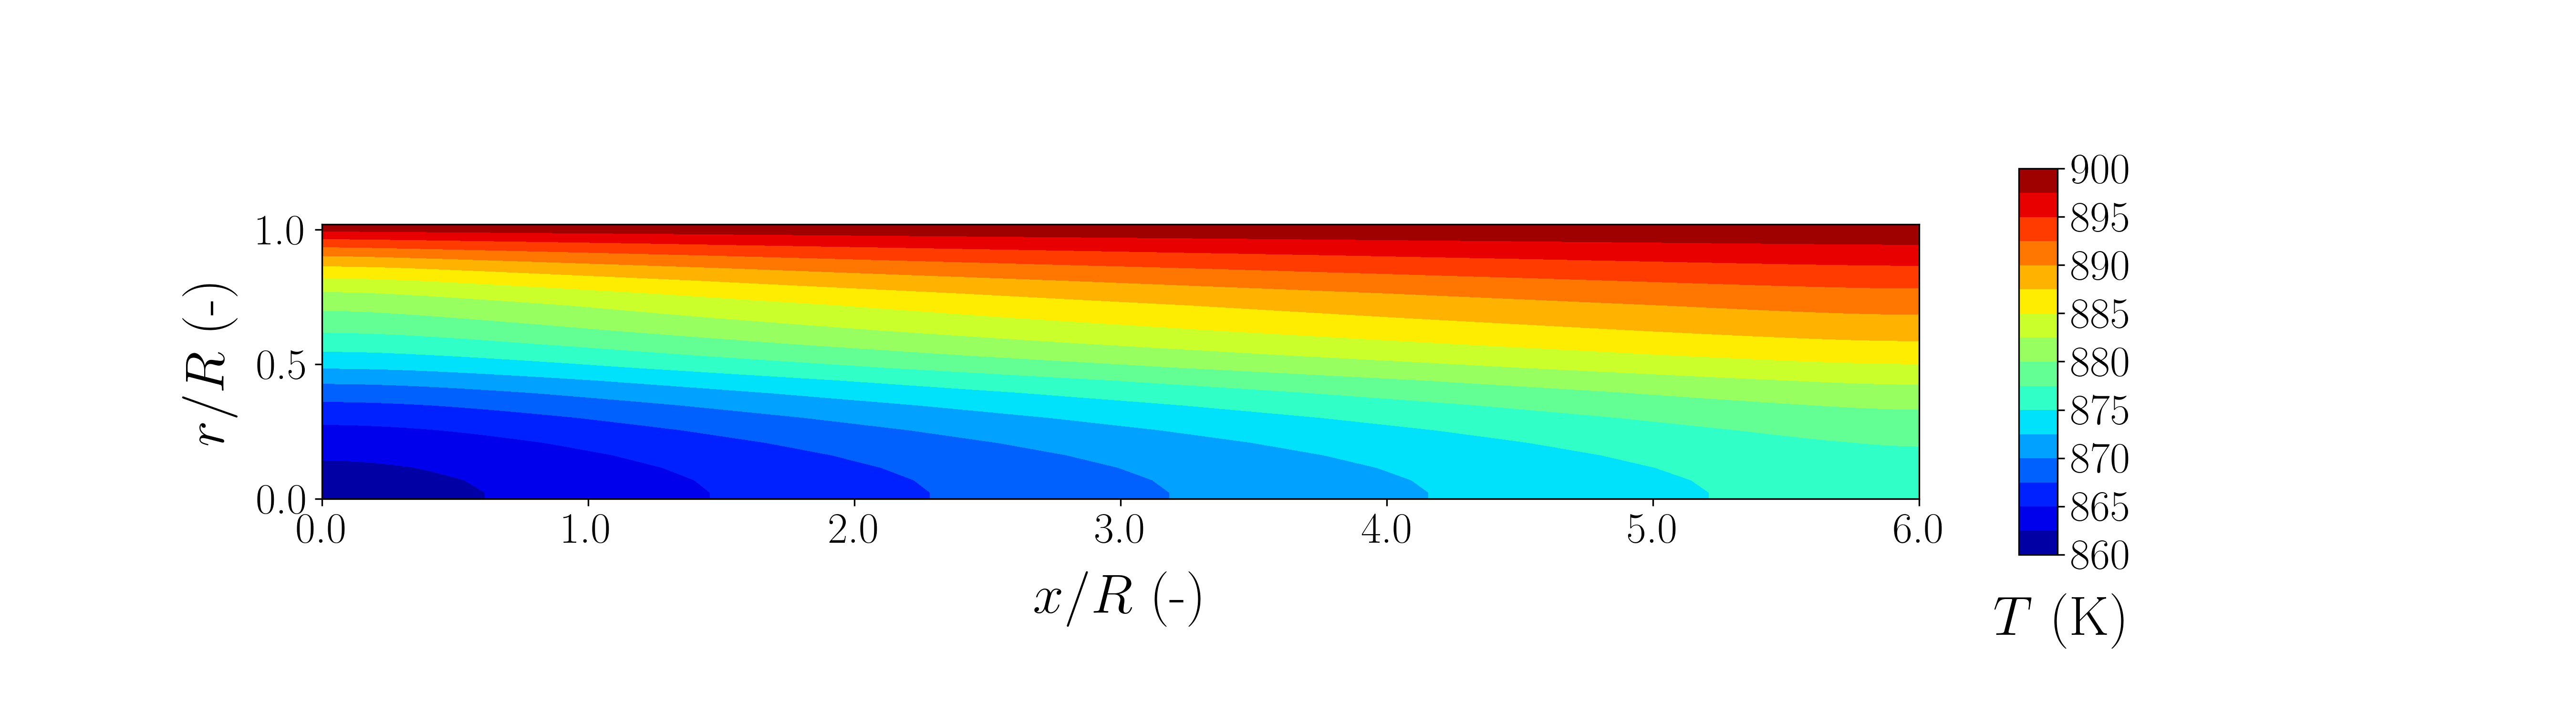
\includegraphics[width=190mm]{results/5Eq/20C_80T/GEN1-TFIELD.png}
%\caption{\label{fig:5RES2080G1-TField} Strategy II - Temperature field distribution - 1$^{\rm{st}}$ generation ($w_{\rm{CH_4}} = 0.2, w_T = 0.8$, $T_{\rm{in}}$ = 900 K, $u_{\rm{in}}$ = 0.15 m s$^{-1}$, $SC$ = 2.0)}
%\end{figure}
%
%\begin{figure}[h!]
%\centering
%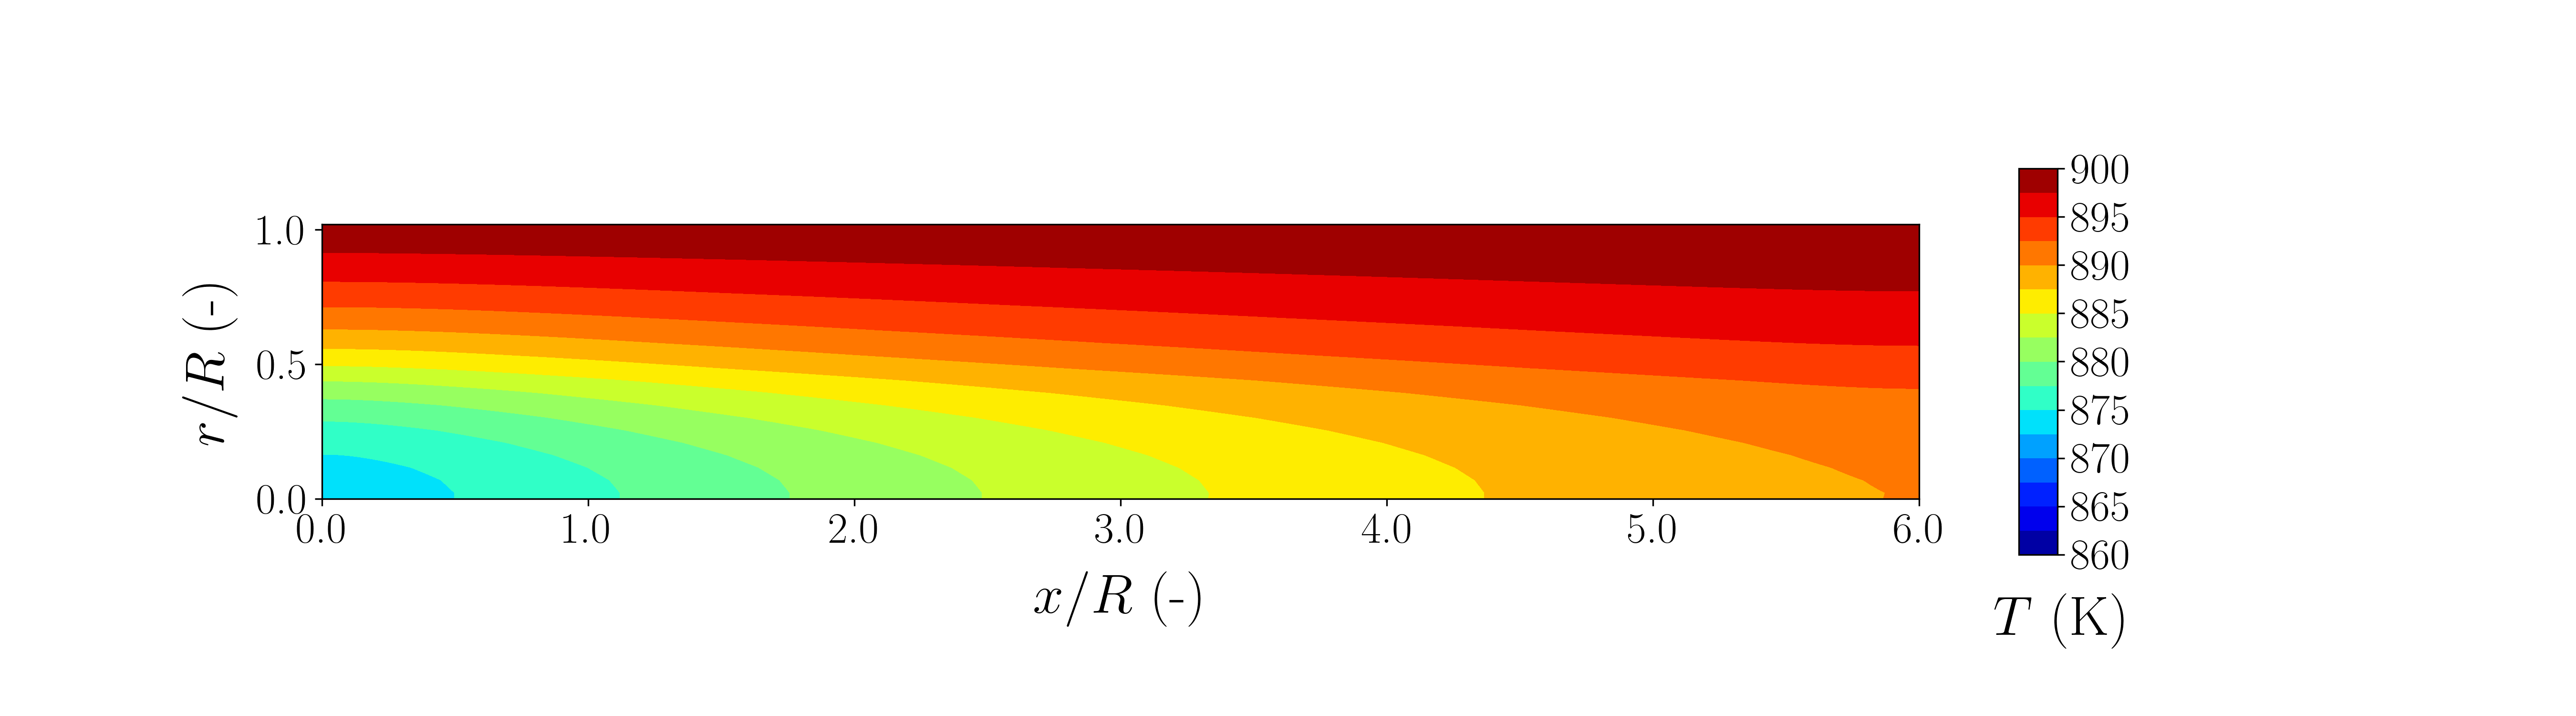
\includegraphics[width=190mm]{results/5Eq/20C_80T/GEN15-TFIELD.png}
%\caption{\label{fig:5RES2080G15-TField} Strategy II - Temperature field distribution - 15$^{\rm{th}}$ generation ($w_{\rm{CH_4}} = 0.2, w_T = 0.8$, $T_{\rm{in}}$ = 900 K, $u_{\rm{in}}$ = 0.15 m s$^{-1}$, $SC$ = 2.0)}
%\end{figure}
%
%\begin{figure}[h!]
%\centering
%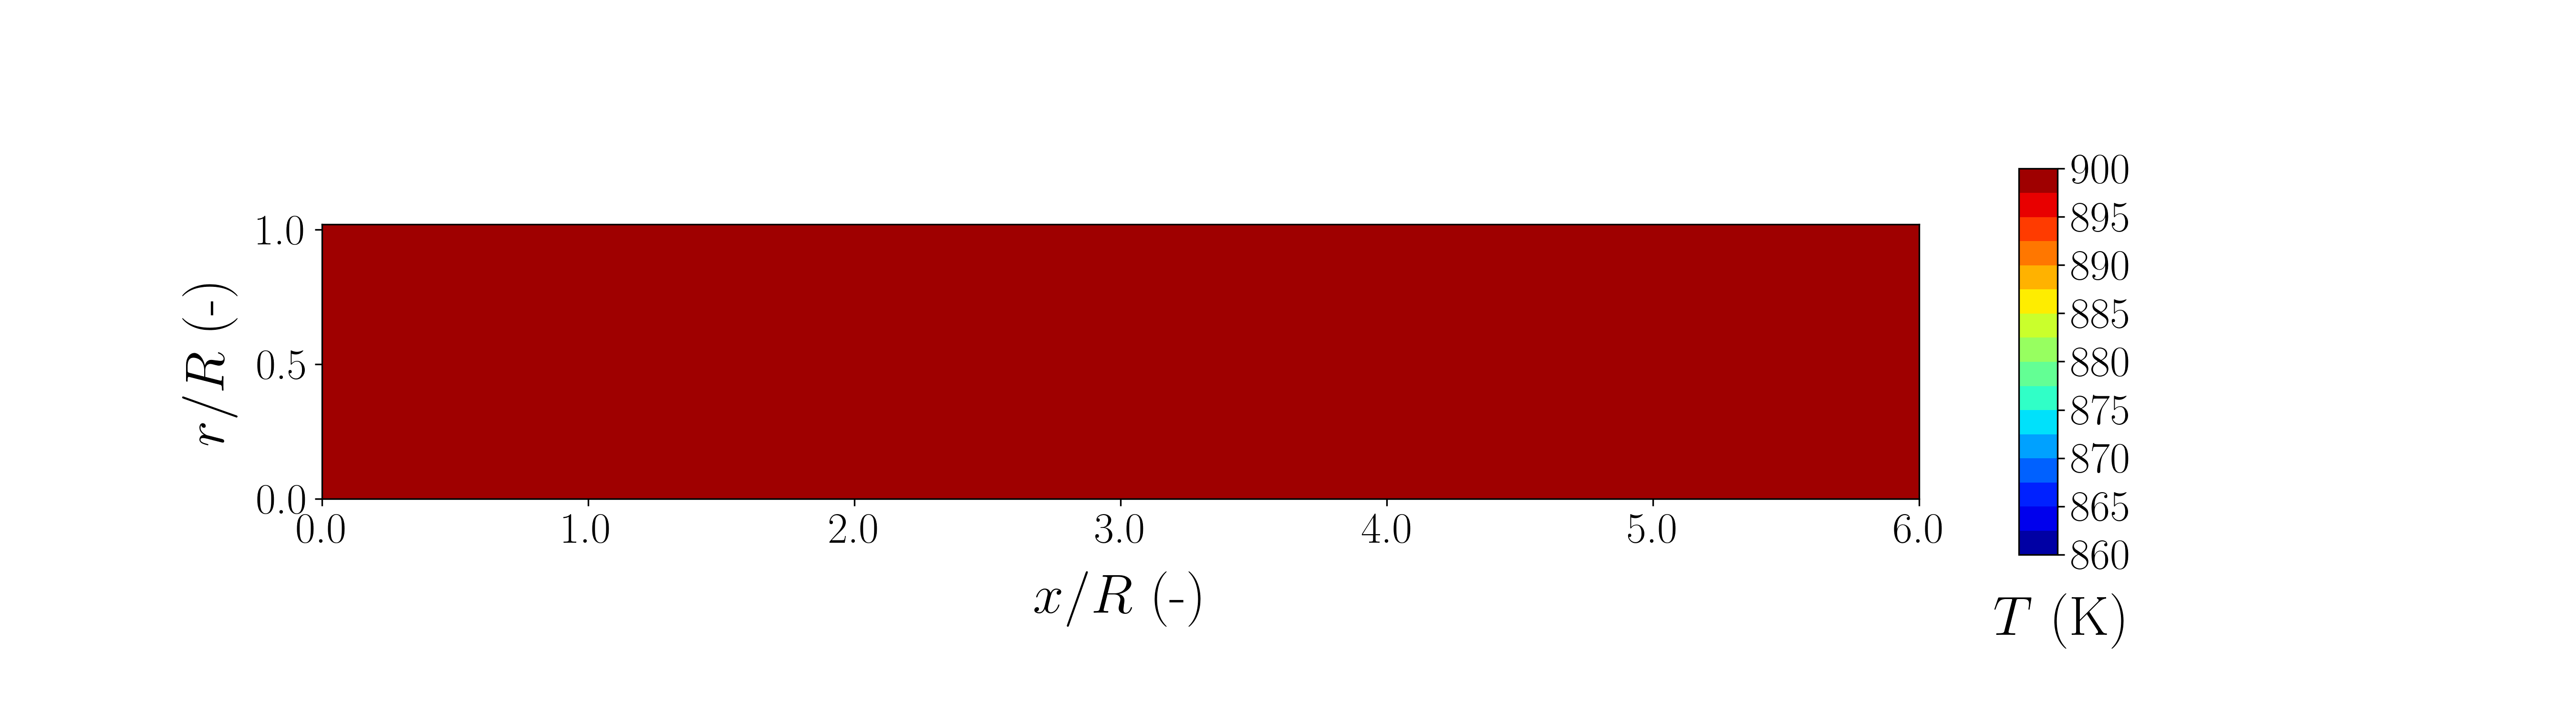
\includegraphics[width=190mm]{results/5Eq/20C_80T/GEN30-TFIELD.png}
%\caption{\label{fig:5RES2080G30-TField} Strategy II - Temperature field distribution - 30$^{\rm{th}}$ generation ($w_{\rm{CH_4}} = 0.2, w_T = 0.8$, $T_{\rm{in}}$ = 900 K, $u_{\rm{in}}$ = 0.15 m s$^{-1}$, $SC$ = 2.0)}
%\end{figure}
%
%
%\begin{figure}[h!]
%\centering
%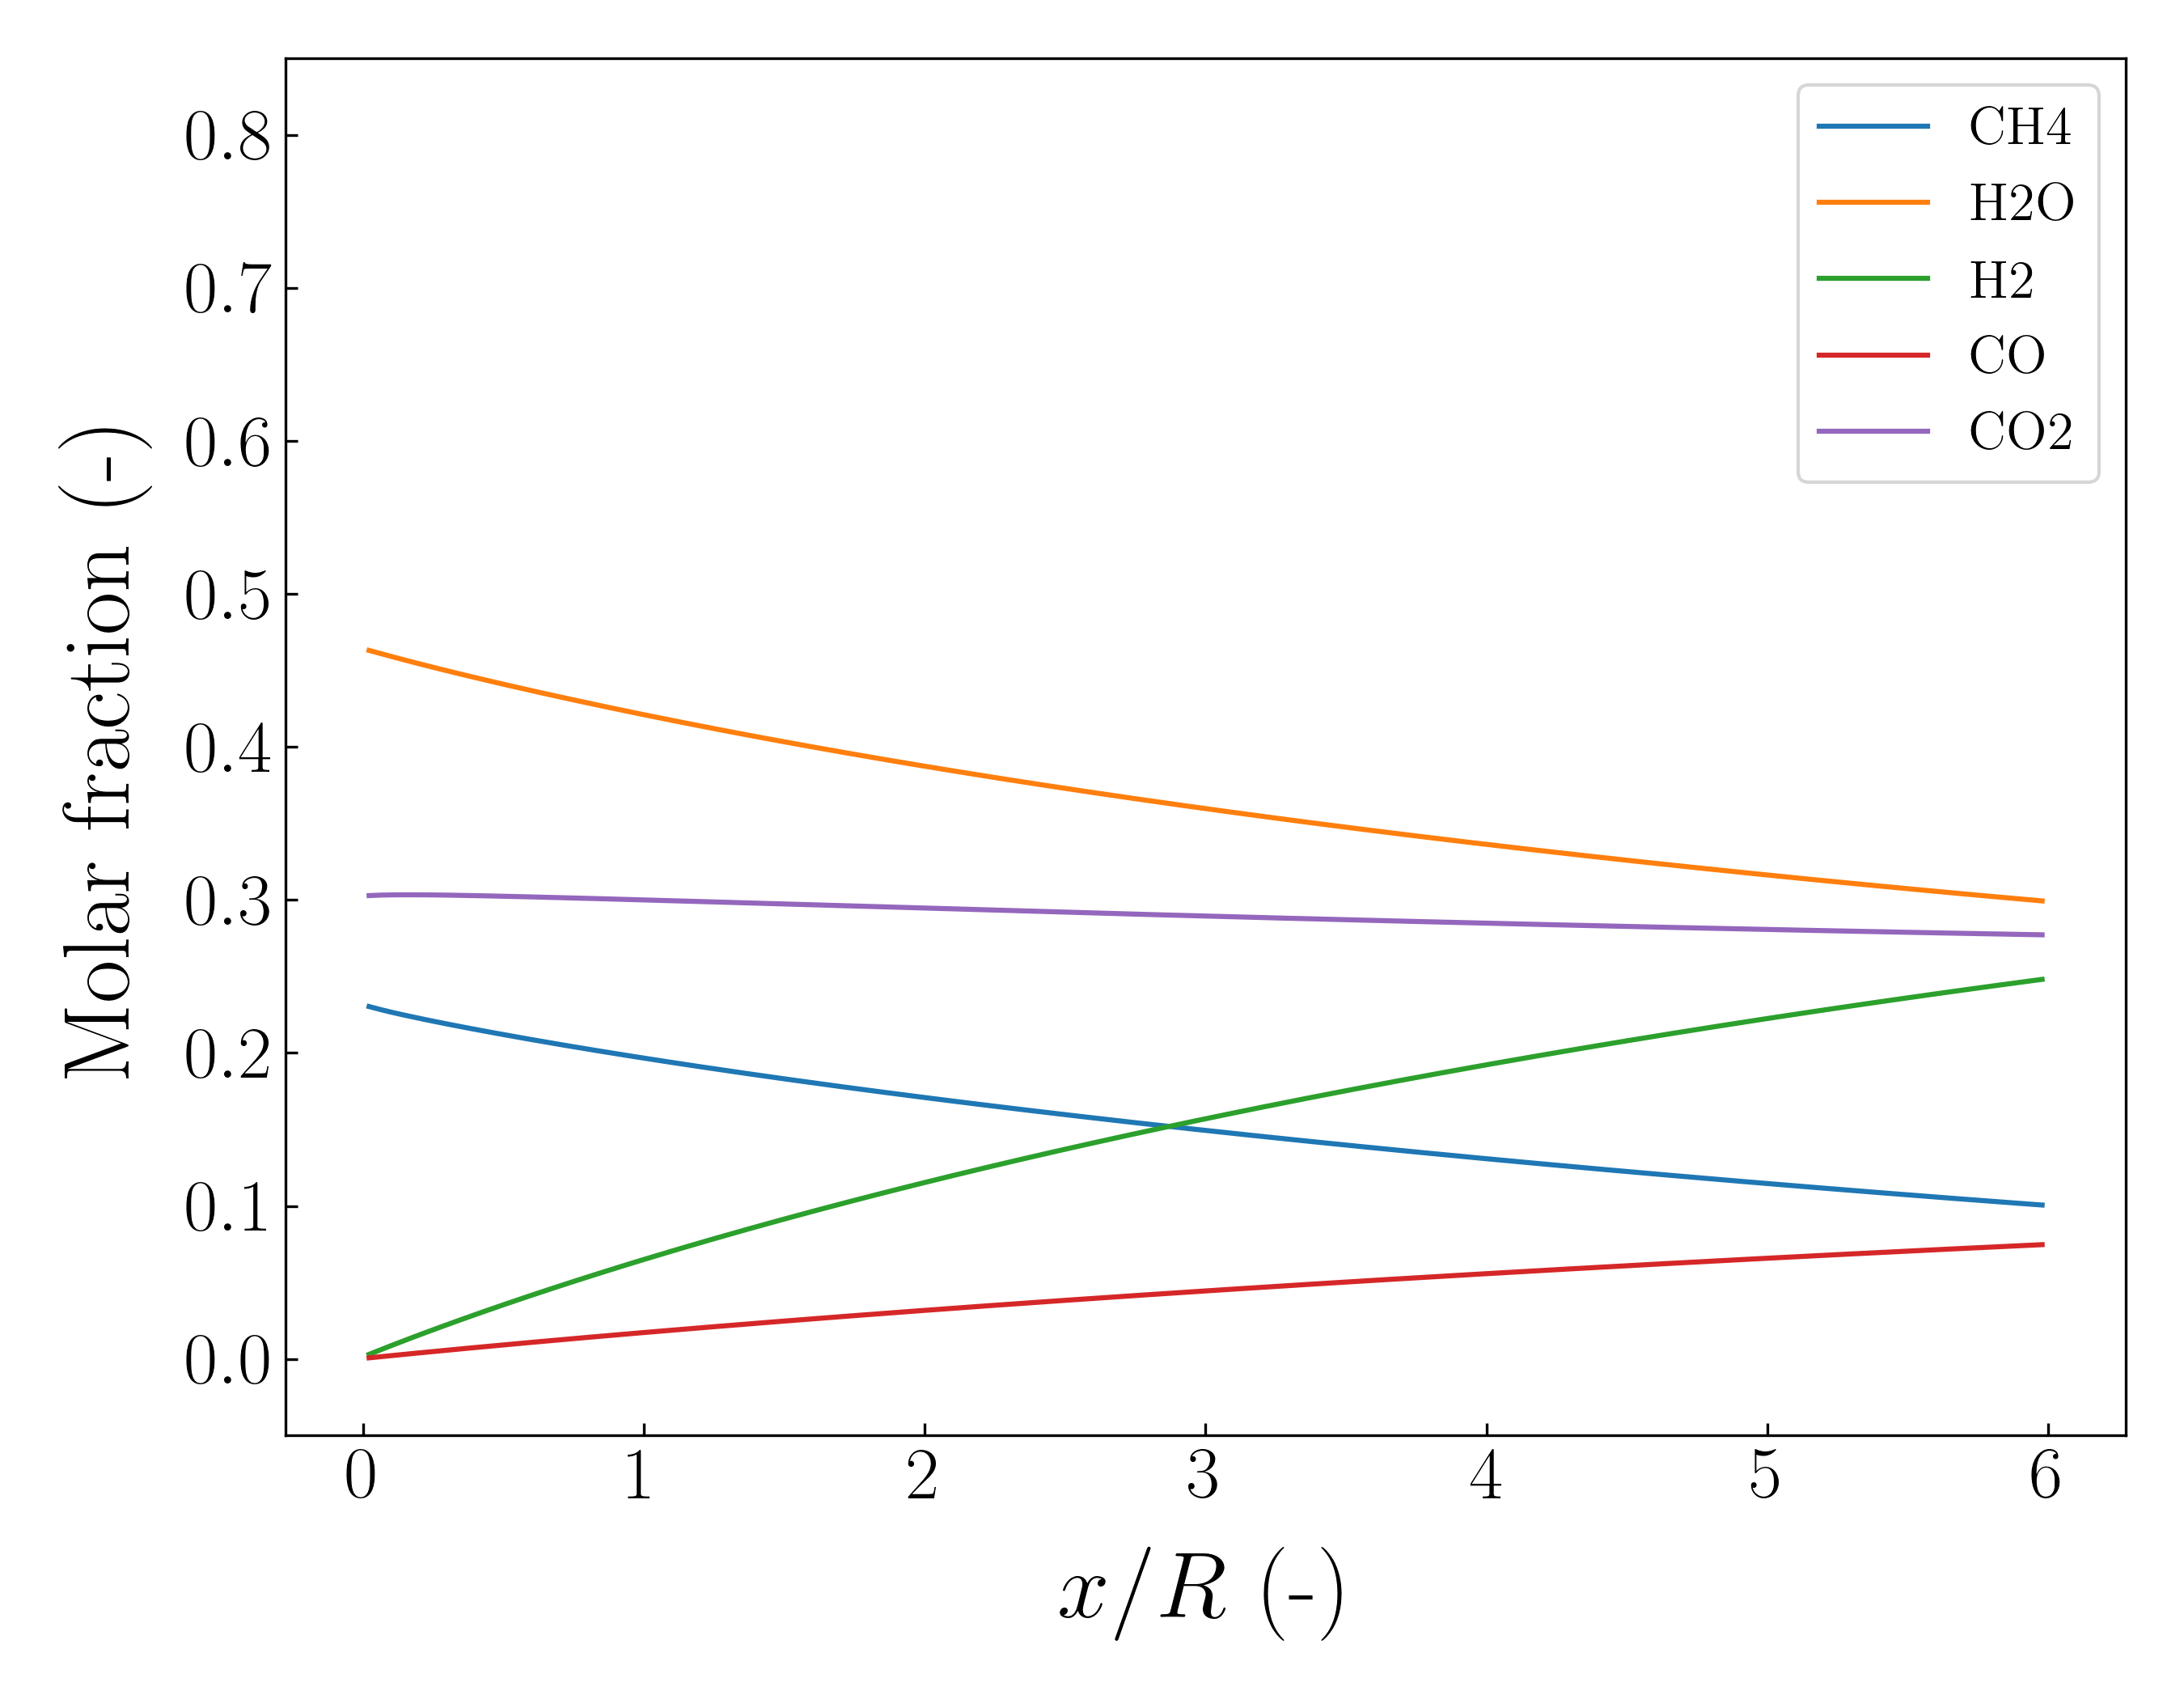
\includegraphics[width=80mm]{results/5Eq/20C_80T/GEN1-AVG.png}
%\caption{\label{fig:5RES2080G1-avg} Strategy II - Radius-averaged molar fractions - 1$^{\rm{st}}$ generation ($w_{\rm{CH_4}} = 0.2, w_T = 0.8$, $T_{\rm{in}}$ = 900 K, $u_{\rm{in}}$ = 0.15 m s$^{-1}$, $SC$ = 2.0)}
%\end{figure}
%
%\begin{figure}[h!]
%\centering
%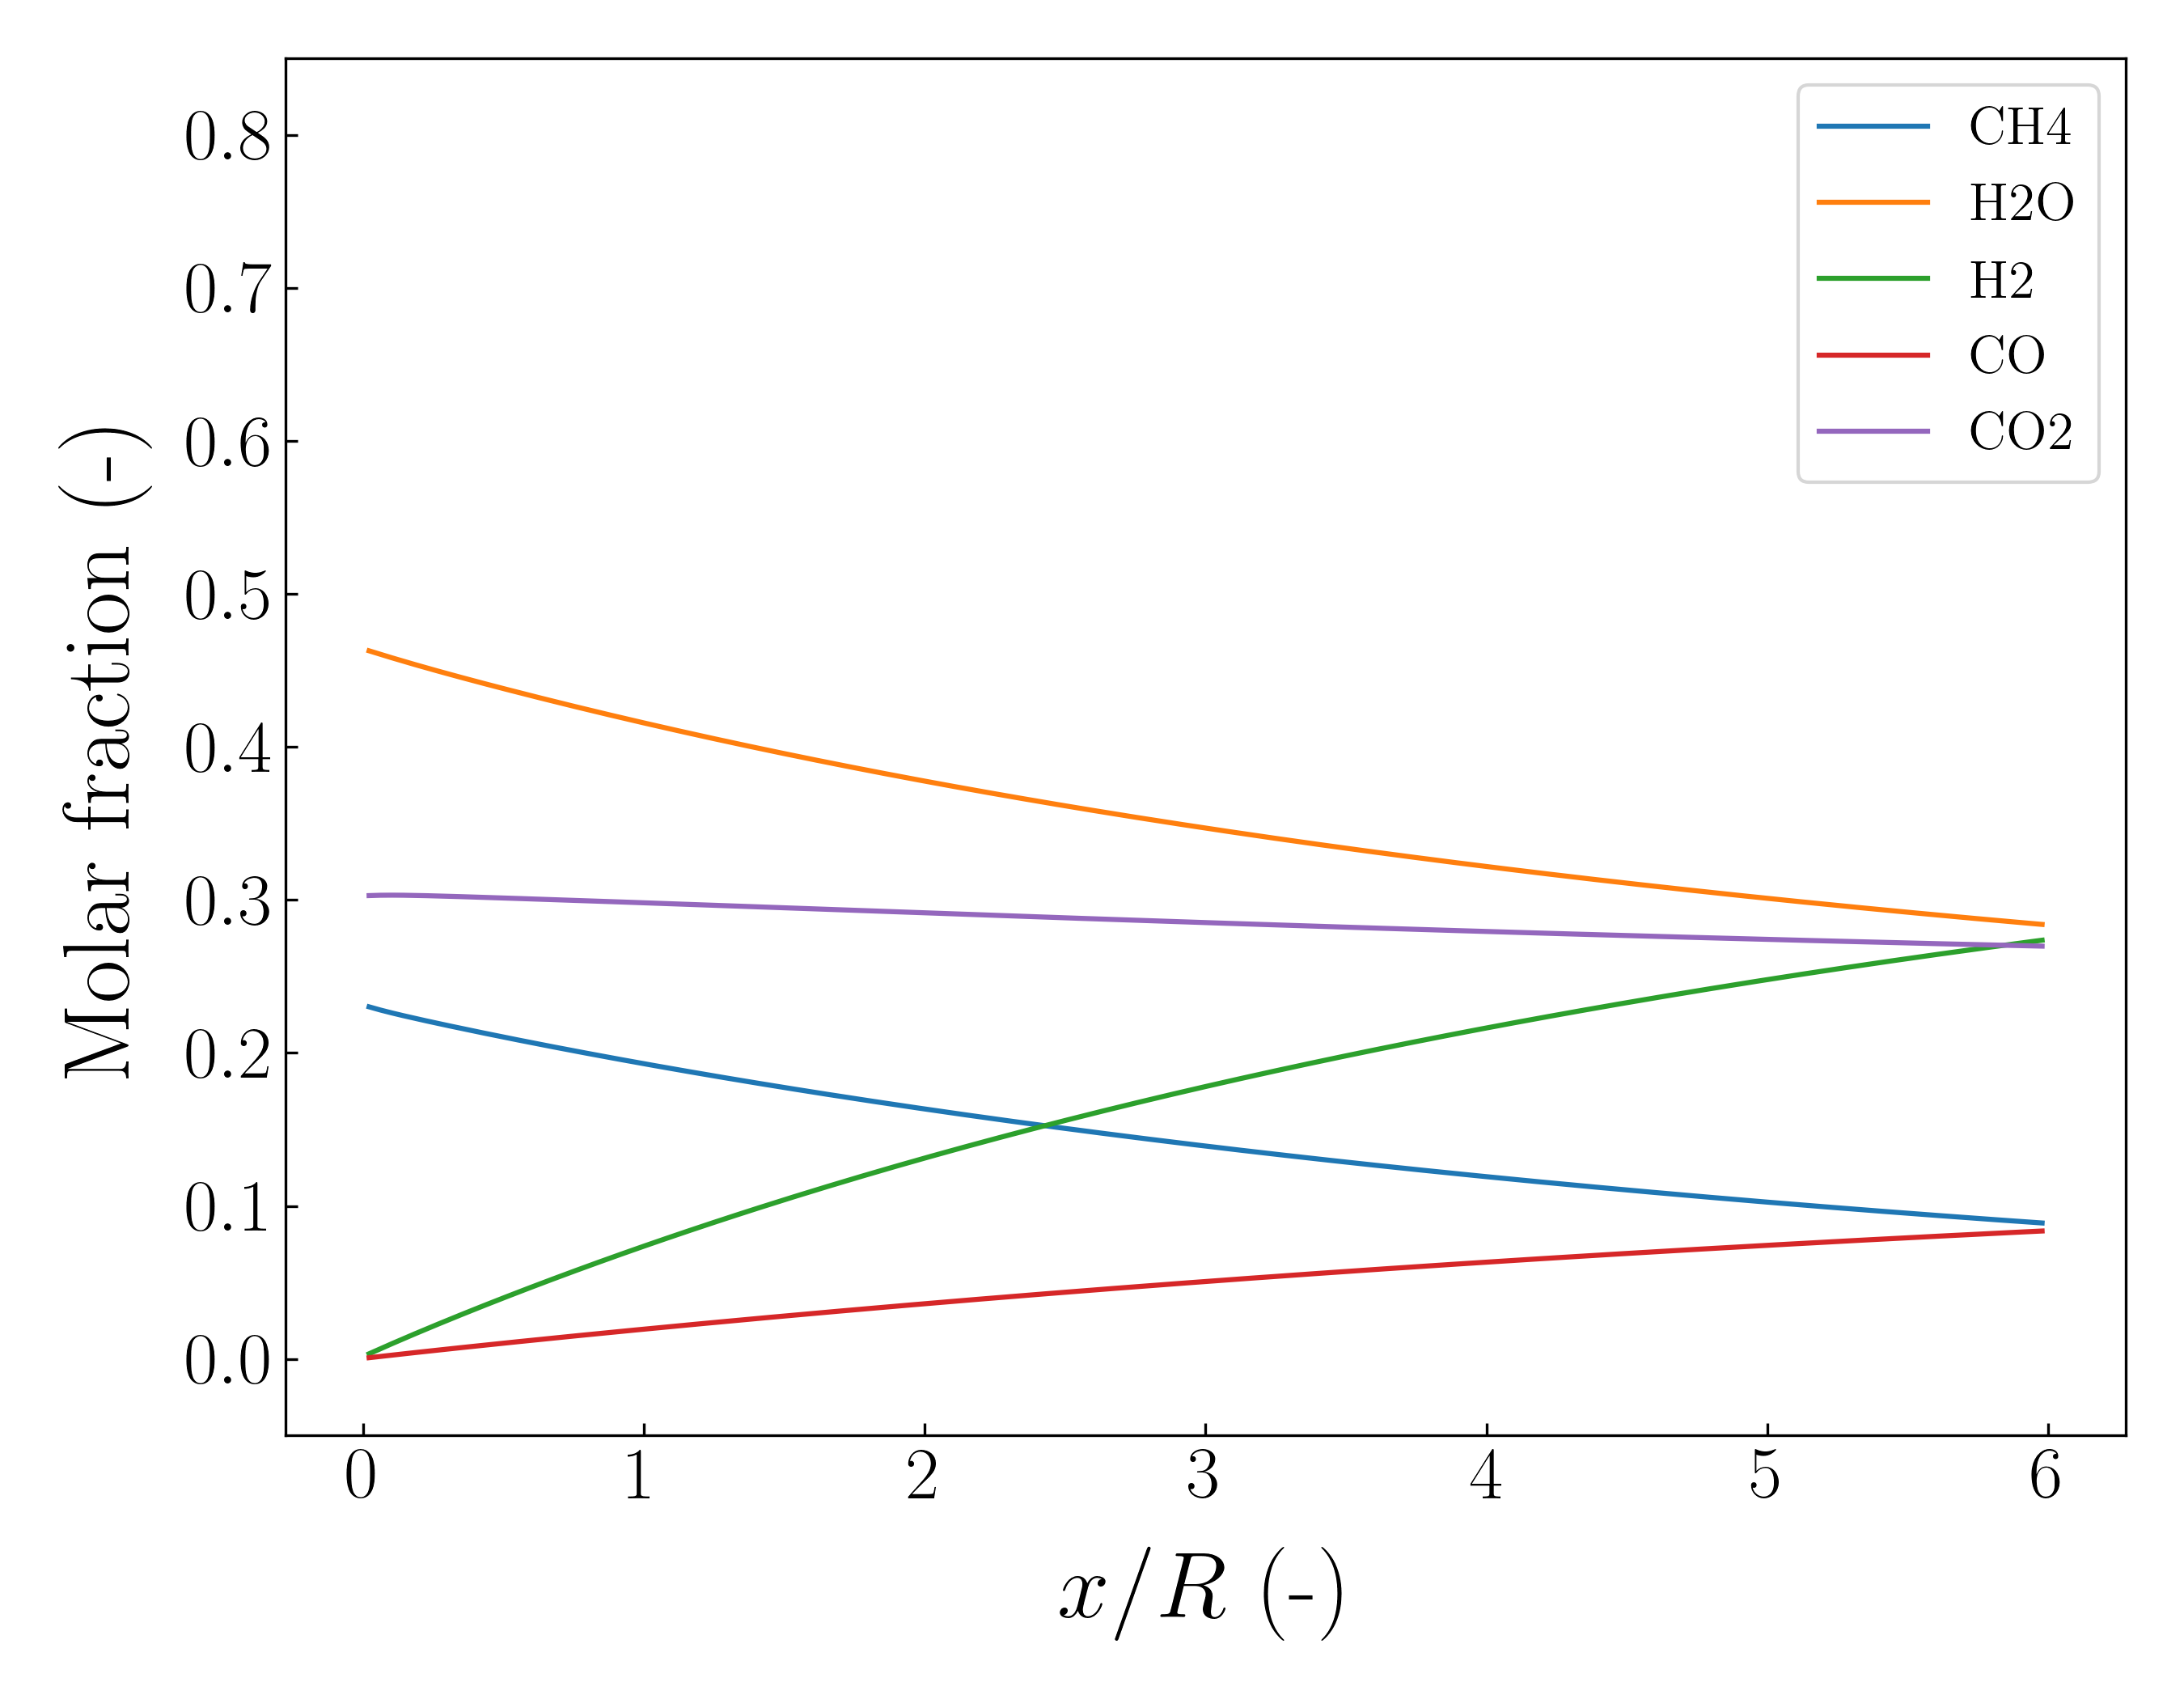
\includegraphics[width=80mm]{results/5Eq/20C_80T/GEN15-AVG.png}
%\caption{\label{fig:5RES2080G15-avg} Strategy II - Radius-averaged molar fractions - 15$^{\rm{th}}$ generation ($w_{\rm{CH_4}} = 0.2, w_T = 0.8$, $T_{\rm{in}}$ = 900 K, $u_{\rm{in}}$ = 0.15 m s$^{-1}$, $SC$ = 2.0)}
%\end{figure}
%
%\begin{figure}[h!]
%\centering
%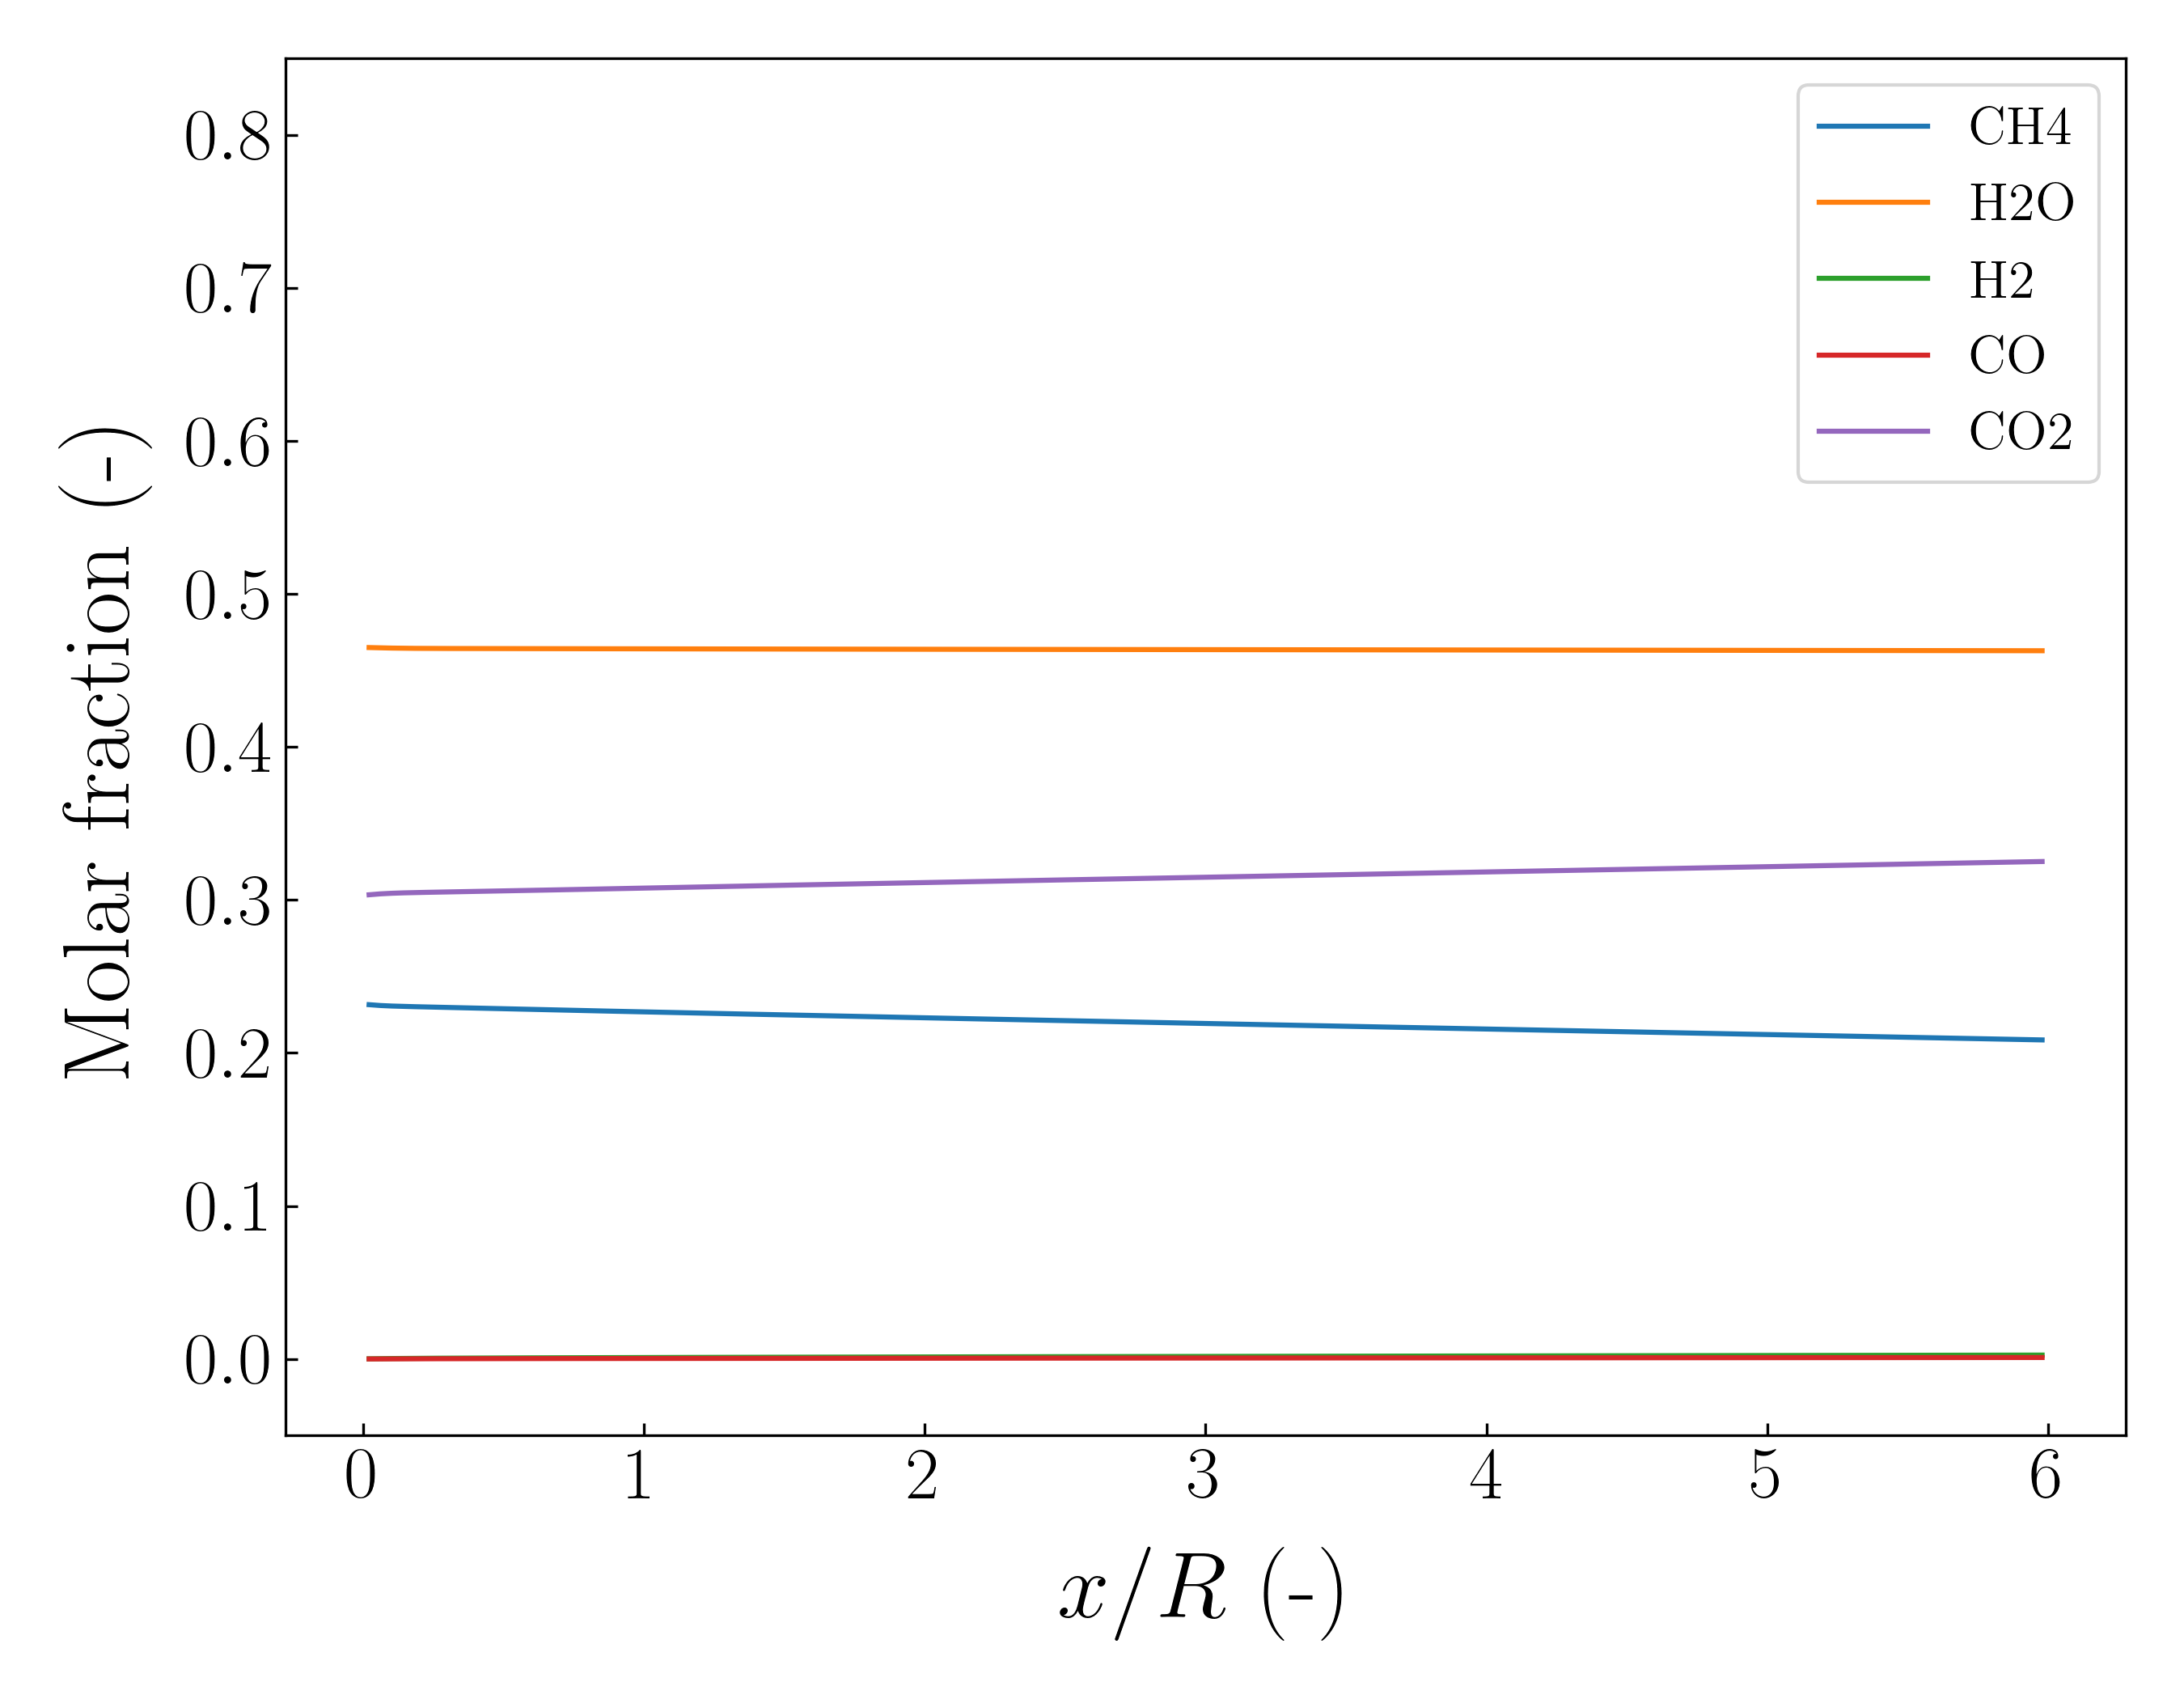
\includegraphics[width=80mm]{results/5Eq/20C_80T/GEN30-AVG.png}
%\caption{\label{fig:5RES2080G30-avg} Strategy II - Radius-averaged molar fractions -  30$^{\rm{th}}$ generation ($w_{\rm{CH_4}} = 0.2, w_T = 0.8$, $T_{\rm{in}}$ = 900 K, $u_{\rm{in}}$ = 0.15 m s$^{-1}$, $SC$ = 2.0)}
%\end{figure}
%
%\begin{figure}[h!]
%\centering
%\includegraphics[width=120mm]{results/segments/5segEq/20C80T/seg.png}
%\caption{\label{fig:30L6040G1-TField} Strategy II - Segments distribution for 30$^{\rm{th}}$ generation ($w_{\rm{CH_4}} = 0.2, w_T = 0.8$, $T_{\rm{in}}$ = 900 K, $u_{\rm{in}}$ = 0.15 m s$^{-1}$, $SC$ = 2.0)}
%\end{figure}
%
%\begin{figure}[h!]
%\centering
%\includegraphics[width=100mm]{results/5Eq/20C_80T.png}
%\caption{\label{fig:5RES2080G-fitness} Strategy II - Fitness analysis throughout successive populations ($w_{\rm{CH_4}} = 0.2, w_T = 0.8$, $T_{\rm{in}}$ = 900 K, $u_{\rm{in}}$ = 0.15 m s$^{-1}$, $SC$ = 2.0)}
%\end{figure}
%
%
%
%\clearpage
%
%
%
%\paragraph{Thermal fitness 60 \%, methane conversion 40 \%} \hspace{0pt} \\
%\noindent 
%
%
%\begin{figure}[h!]
%\centering
%\includegraphics[width=190mm]{results/5Eq/40C_60T/GEN1-TFIELD.png}
%\caption{\label{fig:5RES4060G1-TField} Strategy II - Temperature field distribution - 1$^{\rm{st}}$ generation ($w_{\rm{CH_4}} = 0.4, w_T = 0.6$, $T_{\rm{in}}$ = 900 K, $u_{\rm{in}}$ = 0.15 m s$^{-1}$, $SC$ = 2.0)}
%\end{figure}
%
%\begin{figure}[h!]
%\centering
%\includegraphics[width=190mm]{results/5Eq/40C_60T/GEN15-TFIELD.png}
%\caption{\label{fig:5RES4060G15-TField} Strategy II - Temperature field distribution - 15$^{\rm{th}}$ generation ($w_{\rm{CH_4}} = 0.4, w_T = 0.6$, $T_{\rm{in}}$ = 900 K, $u_{\rm{in}}$ = 0.15 m s$^{-1}$, $SC$ = 2.0)}
%\end{figure}
%
%\begin{figure}[h!]
%\centering
%\includegraphics[width=190mm]{results/5Eq/40C_60T/GEN30-TFIELD.png}
%\caption{\label{fig:5RES4060G30-TField} Strategy II - Temperature field distribution - 30$^{\rm{th}}$ generation ($w_{\rm{CH_4}} = 0.4, w_T = 0.6$, $T_{\rm{in}}$ = 900 K, $u_{\rm{in}}$ = 0.15 m s$^{-1}$, $SC$ = 2.0)}
%\end{figure}
%
%
%\begin{figure}[h!]
%\centering
%\includegraphics[width=80mm]{results/5Eq/40C_60T/GEN1-AVG.png}
%\caption{\label{fig:5RES4060G1-avg} Strategy II - Radius-averaged molar fractions - 1$^{\rm{st}}$ generation ($w_{\rm{CH_4}} = 0.4, w_T = 0.6$, $T_{\rm{in}}$ = 900 K, $u_{\rm{in}}$ = 0.15 m s$^{-1}$, $SC$ = 2.0)}
%\end{figure}
%
%\begin{figure}[h!]
%\centering
%\includegraphics[width=80mm]{results/5Eq/40C_60T/GEN15-AVG.png}
%\caption{\label{fig:5RES4060G15-avg} Strategy II - Radius-averaged molar fractions - 15$^{\rm{th}}$ generation ($w_{\rm{CH_4}} = 0.4, w_T = 0.6$, $T_{\rm{in}}$ = 900 K, $u_{\rm{in}}$ = 0.15 m s$^{-1}$, $SC$ = 2.0)}
%\end{figure}
%
%\begin{figure}[h!]
%\centering
%\includegraphics[width=80mm]{results/5Eq/40C_60T/GEN30-AVG.png}
%\caption{\label{fig:5RES4060G30-avg} Strategy II - Radius-averaged molar fractions -  30$^{\rm{th}}$ generation ($w_{\rm{CH_4}} = 0.4, w_T = 0.6$, $T_{\rm{in}}$ = 900 K, $u_{\rm{in}}$ = 0.15 m s$^{-1}$, $SC$ = 2.0)}
%\end{figure}
%
%\begin{figure}[h!]
%\centering
%\includegraphics[width=120mm]{results/segments/5segEq/40C60T/seg.png}
%\caption{\label{fig:30L6040G1-TField} Strategy II - Segments distribution for 30$^{\rm{th}}$ generation ($w_{\rm{CH_4}} = 0.4, w_T = 0.6$, $T_{\rm{in}}$ = 900 K, $u_{\rm{in}}$ = 0.15 m s$^{-1}$, $SC$ = 2.0)}
%\end{figure}
%
%\begin{figure}[h!]
%\centering
%\includegraphics[width=100mm]{results/5Eq/40C_60T.png}
%\caption{\label{fig:5RES4060G-fitness} Strategy II - Fitness analysis throughout successive populations ($w_{\rm{CH_4}} = 0.4, w_T = 0.6$, $T_{\rm{in}}$ = 900 K, $u_{\rm{in}}$ = 0.15 m s$^{-1}$, $SC$ = 2.0)}
%\end{figure}
%
%
%\clearpage
%
%
%
%
%
%\paragraph{Thermal fitness 50 \%, methane conversion 50 \%} \hspace{0pt} \\
%\noindent 
%
%
%\begin{figure}[h!]
%\centering
%\includegraphics[width=190mm]{results/5Eq/50C_50T/GEN1-TFIELD.png}
%\caption{\label{fig:5RES5050G1-TField} Strategy II - Temperature field distribution - 1$^{\rm{st}}$ generation ($w_{\rm{CH_4}} = 0.5, w_T = 0.5$, $T_{\rm{in}}$ = 900 K, $u_{\rm{in}}$ = 0.15 m s$^{-1}$, $SC$ = 2.0)}
%\end{figure}
%
%\begin{figure}[h!]
%\centering
%\includegraphics[width=190mm]{results/5Eq/50C_50T/GEN15-TFIELD.png}
%\caption{\label{fig:5RES5050G15-TField} Strategy II - Temperature field distribution - 15$^{\rm{th}}$ generation ($w_{\rm{CH_4}} = 0.5, w_T = 0.5$, $T_{\rm{in}}$ = 900 K, $u_{\rm{in}}$ = 0.15 m s$^{-1}$, $SC$ = 2.0)}
%\end{figure}
%
%\begin{figure}[h!]
%\centering
%\includegraphics[width=190mm]{results/5Eq/50C_50T/GEN30-TFIELD.png}
%\caption{\label{fig:5RES5050G30-TField} Strategy II - Temperature field distribution - 30$^{\rm{th}}$ generation ($w_{\rm{CH_4}} = 0.5, w_T = 0.5$, $T_{\rm{in}}$ = 900 K, $u_{\rm{in}}$ = 0.15 m s$^{-1}$, $SC$ = 2.0)}
%\end{figure}
%
%
%\begin{figure}[h!]
%\centering
%\includegraphics[width=80mm]{results/5Eq/50C_50T/GEN1-AVG.png}
%\caption{\label{fig:5RES5050G1-avg} Strategy II - Radius-averaged molar fractions - 1$^{\rm{st}}$ generation ($w_{\rm{CH_4}} = 0.5, w_T = 0.5$, $T_{\rm{in}}$ = 900 K, $u_{\rm{in}}$ = 0.15 m s$^{-1}$, $SC$ = 2.0)}
%\end{figure}
%
%\begin{figure}[h!]
%\centering
%\includegraphics[width=80mm]{results/5Eq/50C_50T/GEN15-AVG.png}
%\caption{\label{fig:5RES5050G15-avg} Strategy II - Radius-averaged molar fractions - 15$^{\rm{th}}$ generation ($w_{\rm{CH_4}} = 0.5, w_T = 0.5$, $T_{\rm{in}}$ = 900 K, $u_{\rm{in}}$ = 0.15 m s$^{-1}$, $SC$ = 2.0)}
%\end{figure}
%
%\begin{figure}[h!]
%\centering
%\includegraphics[width=80mm]{results/5Eq/50C_50T/GEN30-AVG.png}
%\caption{\label{fig:5RES5050G30-avg} Strategy II - Radius-averaged molar fractions -  30$^{\rm{th}}$ generation ($w_{\rm{CH_4}} = 0.5, w_T = 0.5$, $T_{\rm{in}}$ = 900 K, $u_{\rm{in}}$ = 0.15 m s$^{-1}$, $SC$ = 2.0)}
%\end{figure}
%
%\begin{figure}[h!]
%\centering
%\includegraphics[width=120mm]{results/segments/5segEq/50C50T/seg.png}
%\caption{\label{fig:30L6040G1-TField} Strategy II - Segments distribution for 30$^{\rm{th}}$ generation ($w_{\rm{CH_4}} = 0.5, w_T = 0.5$, $T_{\rm{in}}$ = 900 K, $u_{\rm{in}}$ = 0.15 m s$^{-1}$, $SC$ = 2.0)}
%\end{figure}
%
%
%\begin{figure}[h!]
%\centering
%\includegraphics[width=100mm]{results/5Eq/50C_50T.png}
%\caption{\label{fig:5RES5050G-fitness} Strategy II - Fitness analysis throughout successive populations ($w_{\rm{CH_4}} = 0.5, w_T = 0.5$, $T_{\rm{in}}$ = 900 K, $u_{\rm{in}}$ = 0.15 m s$^{-1}$, $SC$ = 2.0)}
%\end{figure}
%
%
%\clearpage
%
%
%
%\paragraph{Thermal fitness 40 \%, methane conversion 60 \%} \hspace{0pt} \\
%\noindent 
%
%
%\begin{figure}[h!]
%\centering
%\includegraphics[width=190mm]{results/5Eq/60C_40T/GEN1-TFIELD.png}
%\caption{\label{fig:5RES6040G1-TField} Strategy II - Temperature field distribution - 1$^{\rm{st}}$ generation ($w_{\rm{CH_4}} = 0.6, w_T = 0.4$, $T_{\rm{in}}$ = 900 K, $u_{\rm{in}}$ = 0.15 m s$^{-1}$, $SC$ = 2.0)}
%\end{figure}
%
%\begin{figure}[h!]
%\centering
%\includegraphics[width=190mm]{results/5Eq/60C_40T/GEN15-TFIELD.png}
%\caption{\label{fig:5RES6040G15-TField} Strategy II - Temperature field distribution - 15$^{\rm{th}}$ generation ($w_{\rm{CH_4}} = 0.6, w_T = 0.4$, $T_{\rm{in}}$ = 900 K, $u_{\rm{in}}$ = 0.15 m s$^{-1}$, $SC$ = 2.0)}
%\end{figure}
%
%\begin{figure}[h!]
%\centering
%\includegraphics[width=190mm]{results/5Eq/60C_40T/GEN30-TFIELD.png}
%\caption{\label{fig:5RES6040G30-TField} Strategy II - Temperature field distribution - 30$^{\rm{th}}$ generation ($w_{\rm{CH_4}} = 0.6, w_T = 0.4$, $T_{\rm{in}}$ = 900 K, $u_{\rm{in}}$ = 0.15 m s$^{-1}$, $SC$ = 2.0)}
%\end{figure}
%
%
%\begin{figure}[h!]
%\centering
%\includegraphics[width=80mm]{results/5Eq/60C_40T/GEN1-AVG.png}
%\caption{\label{fig:5RES6040G1-avg} Strategy II - Radius-averaged molar fractions - 1$^{\rm{st}}$ generation ($w_{\rm{CH_4}} = 0.6, w_T = 0.4$, $T_{\rm{in}}$ = 900 K, $u_{\rm{in}}$ = 0.15 m s$^{-1}$, $SC$ = 2.0)}
%\end{figure}
%
%\begin{figure}[h!]
%\centering
%\includegraphics[width=80mm]{results/5Eq/60C_40T/GEN15-AVG.png}
%\caption{\label{fig:5RES6040G15-avg} Strategy II - Radius-averaged molar fractions - 15$^{\rm{th}}$ generation ($w_{\rm{CH_4}} = 0.6, w_T = 0.4$, $T_{\rm{in}}$ = 900 K, $u_{\rm{in}}$ = 0.15 m s$^{-1}$, $SC$ = 2.0)}
%\end{figure}
%
%\begin{figure}[h!]
%\centering
%\includegraphics[width=80mm]{results/5Eq/60C_40T/GEN30-AVG.png}
%\caption{\label{fig:5RES6040G30-avg} Strategy II - Radius-averaged molar fractions -  30$^{\rm{th}}$ generation ($w_{\rm{CH_4}} = 0.6, w_T = 0.4$, $T_{\rm{in}}$ = 900 K, $u_{\rm{in}}$ = 0.15 m s$^{-1}$, $SC$ = 2.0)}
%\end{figure}
%
%\begin{figure}[h!]
%\centering
%\includegraphics[width=120mm]{results/segments/5segEq/60C40T/seg.png}
%\caption{\label{fig:30L6040G1-TField} Strategy II - Segments distribution for 30$^{\rm{th}}$ generation ($w_{\rm{CH_4}} = 0.6, w_T = 0.4$, $T_{\rm{in}}$ = 900 K, $u_{\rm{in}}$ = 0.15 m s$^{-1}$, $SC$ = 2.0)}
%\end{figure}
%
%\begin{figure}[h!]
%\centering
%\includegraphics[width=100mm]{results/5Eq/60C_40T.png}
%\caption{\label{fig:5RES6040G-fitness} Strategy II - Fitness analysis throughout successive populations ($w_{\rm{CH_4}} = 0.6, w_T = 0.4$, $T_{\rm{in}}$ = 900 K, $u_{\rm{in}}$ = 0.15 m s$^{-1}$, $SC$ = 2.0)}
%\end{figure}
%
%\clearpage
%
%
%\paragraph{Thermal fitness 20 \%, methane conversion 80 \%} \hspace{0pt} \\
%\noindent 
%
%
%
%\begin{figure}[h!]
%\centering
%\includegraphics[width=190mm]{results/5Eq/80C_20T/GEN1-TFIELD.png}
%\caption{\label{fig:5RES8020G1-TField} Strategy II - Temperature field distribution - 1$^{\rm{st}}$ generation ($w_{\rm{CH_4}} = 0.8, w_T = 0.2$, $T_{\rm{in}}$ = 900 K, $u_{\rm{in}}$ = 0.15 m s$^{-1}$, $SC$ = 2.0)}
%\end{figure}
%
%\begin{figure}[h!]
%\centering
%\includegraphics[width=190mm]{results/5Eq/80C_20T/GEN15-TFIELD.png}
%\caption{\label{fig:5RES8020G15-TField} Strategy II - Temperature field distribution - 15$^{\rm{th}}$ generation ($w_{\rm{CH_4}} = 0.8, w_T = 0.2$, $T_{\rm{in}}$ = 900 K, $u_{\rm{in}}$ = 0.15 m s$^{-1}$, $SC$ = 2.0)}
%\end{figure}
%
%\begin{figure}[h!]
%\centering
%\includegraphics[width=190mm]{results/5Eq/80C_20T/GEN30-TFIELD.png}
%\caption{\label{fig:5RES8020G30-TField} Strategy II - Temperature field distribution - 30$^{\rm{th}}$ generation ($w_{\rm{CH_4}} = 0.8, w_T = 0.2$, $T_{\rm{in}}$ = 900 K, $u_{\rm{in}}$ = 0.15 m s$^{-1}$, $SC$ = 2.0)}
%\end{figure}
%
%
%\begin{figure}[h!]
%\centering
%\includegraphics[width=80mm]{results/5Eq/80C_20T/GEN1-AVG.png}
%\caption{\label{fig:5RES8020G1-avg} Strategy II - Radius-averaged molar fractions - 1$^{\rm{st}}$ generation ($w_{\rm{CH_4}} = 0.8, w_T = 0.2$, $T_{\rm{in}}$ = 900 K, $u_{\rm{in}}$ = 0.15 m s$^{-1}$, $SC$ = 2.0)}
%\end{figure}
%
%\begin{figure}[h!]
%\centering
%\includegraphics[width=80mm]{results/5Eq/80C_20T/GEN15-AVG.png}
%\caption{\label{fig:5RES8020G15-avg} Strategy II - Radius-averaged molar fractions - 15$^{\rm{th}}$ generation ($w_{\rm{CH_4}} = 0.8, w_T = 0.2$, $T_{\rm{in}}$ = 900 K, $u_{\rm{in}}$ = 0.15 m s$^{-1}$, $SC$ = 2.0)}
%\end{figure}
%
%\begin{figure}[h!]
%\centering
%\includegraphics[width=120mm]{results/segments/5segEq/80C20T/seg.png}
%\caption{\label{fig:30L6040G1-TField} Strategy II - Segments distribution for 30$^{\rm{th}}$ generation ($w_{\rm{CH_4}} = 0.8, w_T = 0.2$, $T_{\rm{in}}$ = 900 K, $u_{\rm{in}}$ = 0.15 m s$^{-1}$, $SC$ = 2.0)}
%\end{figure}
%
%\begin{figure}[h!]
%\centering
%\includegraphics[width=80mm]{results/5Eq/80C_20T/GEN30-AVG.png}
%\caption{\label{fig:5RES8020G30-avg} Strategy II - Radius-averaged molar fractions -  30$^{\rm{th}}$ generation ($w_{\rm{CH_4}} = 0.8, w_T = 0.2$, $T_{\rm{in}}$ = 900 K, $u_{\rm{in}}$ = 0.15 m s$^{-1}$, $SC$ = 2.0)}
%\end{figure}
%
%
%\begin{figure}[h!]
%\centering
%\includegraphics[width=100mm]{results/5Eq/80C_20T.png}
%\caption{\label{fig:5RES8020G-fitness} Strategy II - Fitness analysis throughout successive populations ($w_{\rm{CH_4}} = 0.8, w_T = 0.2$, $T_{\rm{in}}$ = 900 K, $u_{\rm{in}}$ = 0.15 m s$^{-1}$, $SC$ = 2.0)}
%\end{figure}
%
%\begin{center}
%\begin{table}
%\centering
%\caption{Hydrogen productivity for the catalytic insert division strategy II}
%\label{tab:5RH2prod}
%\begin{tabular}{l|c|c|c}
%\hline\noalign{\smallskip}
% $w_{\rm{CH_4}}$ / $ w_T $ & $\rm{H_{2_{out}}}$ & $\iota$ & $\zeta$ \\
%\noalign{\smallskip}\hline\noalign{\smallskip}
%REF         & 0.581     & 1.00  &  0.581\\
%0.2 / 0.8   & 0.001     & 0.00  & N / A \\
%0.4 / 0.6   & 0.492     & 0.32  & 1.527 \\
%0.5 / 0.5   & 0.175     & 0.32  & 0.548 \\
%0.6 / 0.4   & 0.536     & 0.53  & 1.616 \\
%0.8 / 0.2   & 0.200     & 0.27  & 0.744 \\
%\noalign{\smallskip}\hline
%\end{tabular}
%\end{table}
%\end{center}

\section{Conclusions}


%% The Appendices part is started with the command \appendix;
%% appendix sections are then done as normal sections
%% \appendix

%% \section{}
%% \label{}

%% For citations use: 
%%       \citet{<label>} ==> Jones et al. [21]
%%       \citep{<label>} ==> [21]
%%

%% If you have bibdatabase file and want bibtex to generate the
%% bibitems, please use
%%

\clearpage

\bibliographystyle{elsarticle-num-names} 
\bibliography{bib1.bib}

%% else use the following coding to input the bibitems directly in the
%% TeX file.

\begin{thebibliography}{00}

%% \bibitem[Author(year)]{label}
%% Text of bibliographic item

%\bibitem[ ()]{}

\end{thebibliography}
\end{document}

\endinput
%%
%% End of file `elsarticle-template-num-names.tex'.
